% Options for packages loaded elsewhere
\PassOptionsToPackage{unicode}{hyperref}
\PassOptionsToPackage{hyphens}{url}
%
\documentclass[
  12pt,
  french,
]{article}
\usepackage{amsmath,amssymb}
\usepackage{lmodern}
\usepackage{ifxetex,ifluatex}
\ifnum 0\ifxetex 1\fi\ifluatex 1\fi=0 % if pdftex
  \usepackage[T1]{fontenc}
  \usepackage[utf8]{inputenc}
  \usepackage{textcomp} % provide euro and other symbols
\else % if luatex or xetex
  \usepackage{unicode-math}
  \defaultfontfeatures{Scale=MatchLowercase}
  \defaultfontfeatures[\rmfamily]{Ligatures=TeX,Scale=1}
\fi
% Use upquote if available, for straight quotes in verbatim environments
\IfFileExists{upquote.sty}{\usepackage{upquote}}{}
\IfFileExists{microtype.sty}{% use microtype if available
  \usepackage[]{microtype}
  \UseMicrotypeSet[protrusion]{basicmath} % disable protrusion for tt fonts
}{}
\makeatletter
\@ifundefined{KOMAClassName}{% if non-KOMA class
  \IfFileExists{parskip.sty}{%
    \usepackage{parskip}
  }{% else
    \setlength{\parindent}{0pt}
    \setlength{\parskip}{6pt plus 2pt minus 1pt}}
}{% if KOMA class
  \KOMAoptions{parskip=half}}
\makeatother
\usepackage{xcolor}
\IfFileExists{xurl.sty}{\usepackage{xurl}}{} % add URL line breaks if available
\IfFileExists{bookmark.sty}{\usepackage{bookmark}}{\usepackage{hyperref}}
\hypersetup{
  pdflang={fr},
  hidelinks,
  pdfcreator={LaTeX via pandoc}}
\urlstyle{same} % disable monospaced font for URLs
\usepackage[left = 2.5cm, right = 2cm, top = 2cm, bottom =
2cm]{geometry}
\usepackage{longtable,booktabs,array}
\usepackage{calc} % for calculating minipage widths
% Correct order of tables after \paragraph or \subparagraph
\usepackage{etoolbox}
\makeatletter
\patchcmd\longtable{\par}{\if@noskipsec\mbox{}\fi\par}{}{}
\makeatother
% Allow footnotes in longtable head/foot
\IfFileExists{footnotehyper.sty}{\usepackage{footnotehyper}}{\usepackage{footnote}}
\makesavenoteenv{longtable}
\usepackage{graphicx}
\makeatletter
\def\maxwidth{\ifdim\Gin@nat@width>\linewidth\linewidth\else\Gin@nat@width\fi}
\def\maxheight{\ifdim\Gin@nat@height>\textheight\textheight\else\Gin@nat@height\fi}
\makeatother
% Scale images if necessary, so that they will not overflow the page
% margins by default, and it is still possible to overwrite the defaults
% using explicit options in \includegraphics[width, height, ...]{}
\setkeys{Gin}{width=\maxwidth,height=\maxheight,keepaspectratio}
% Set default figure placement to htbp
\makeatletter
\def\fps@figure{htbp}
\makeatother
\usepackage[normalem]{ulem}
% Avoid problems with \sout in headers with hyperref
\pdfstringdefDisableCommands{\renewcommand{\sout}{}}
\setlength{\emergencystretch}{3em} % prevent overfull lines
\providecommand{\tightlist}{%
  \setlength{\itemsep}{0pt}\setlength{\parskip}{0pt}}
\setcounter{secnumdepth}{-\maxdimen} % remove section numbering
\usepackage{float}
\usepackage{sectsty}
\usepackage{paralist}
\usepackage{setspace}\spacing{1.5}
\usepackage{fancyhdr}
\usepackage{lastpage}
\usepackage{dcolumn}
\usepackage{endnotes} \let\footnote=\endnote
\usepackage{natbib} \bibliographystyle{apalike}
\usepackage[nottoc, numbib]{tocbibind}
\usepackage{lscape}
\newcommand{\blandscape}{\begin{landscape}}
\newcommand{\elandscape}{\end{landscape}}
\usepackage{bm}
\ifxetex
  % Load polyglossia as late as possible: uses bidi with RTL langages (e.g. Hebrew, Arabic)
  \usepackage{polyglossia}
  \setmainlanguage[]{french}
\else
  \usepackage[main=french]{babel}
% get rid of language-specific shorthands (see #6817):
\let\LanguageShortHands\languageshorthands
\def\languageshorthands#1{}
\fi
\ifluatex
  \usepackage{selnolig}  % disable illegal ligatures
\fi
\newlength{\cslhangindent}
\setlength{\cslhangindent}{1.5em}
\newlength{\csllabelwidth}
\setlength{\csllabelwidth}{3em}
\newenvironment{CSLReferences}[2] % #1 hanging-ident, #2 entry spacing
 {% don't indent paragraphs
  \setlength{\parindent}{0pt}
  % turn on hanging indent if param 1 is 1
  \ifodd #1 \everypar{\setlength{\hangindent}{\cslhangindent}}\ignorespaces\fi
  % set entry spacing
  \ifnum #2 > 0
  \setlength{\parskip}{#2\baselineskip}
  \fi
 }%
 {}
\usepackage{calc}
\newcommand{\CSLBlock}[1]{#1\hfill\break}
\newcommand{\CSLLeftMargin}[1]{\parbox[t]{\csllabelwidth}{#1}}
\newcommand{\CSLRightInline}[1]{\parbox[t]{\linewidth - \csllabelwidth}{#1}\break}
\newcommand{\CSLIndent}[1]{\hspace{\cslhangindent}#1}

\author{}
\date{\vspace{-2.5em}}

\begin{document}

\allsectionsfont{\centering}
\subsectionfont{\raggedright}
\subsubsectionfont{\raggedright}

\pagenumbering{gobble}

\begin{centering}

\vspace{3cm}



\includegraphics[width=0.2\linewidth]{C:/Users/Admin/OneDrive/Documents/Github projects/thesis/Logo} 

\vspace{1cm}

\Large
{\bf Université Libre de Bruxelles}

\Large
{\bf Faculté des Sciences Psychologiques et de l'Education}

\vspace{1cm}

\Large

\doublespacing
{\bf METHODE EN PSYCHOLOGIE : \\OUTILS ET RECOMMANDATIONS POUR COMPRENDRE ET GERER LES HYPOTHESES, CONDITIONS D'APPLICATION DES TESTS ET LES MESURES DE TAILLE D'EFFETS}

\vspace{1 cm}

\normalsize
\singlespacing
Par

\vspace{0.5 cm}

\Large

{\bf MARIE DELACRE}

\vspace{1.5 cm}

En vue de l'obtention du grade de docteur

\vspace{1.5 cm}

\normalsize
Septembre 2021

\end{centering}

\newpage

\pagenumbering{gobble}

\begin{centering}

{\bf Abstract}

\end{centering}

\spacing{1.5}

Abstract (voir nombre de mots requis)

\pagenumbering{roman}

\newpage

\newpage

\tableofcontents
\addtocontents{toc}{\protect\setcounter{tocdepth}{1}}

\newpage

\section*{Remerciements}

Thank you for following this tutorial!

I hope you'll find it useful to write a very professional dissertation.

\newpage

\pagenumbering{arabic}

\bibliographystyle{apalike-fr}

\hypertarget{chapitre-1-introduction}{%
\section{Chapitre 1: Introduction}\label{chapitre-1-introduction}}

On attend des chercheurs en psychologie, et des psychologues en général,
qu'ils soient capables de produire des connaissances fondées sur des
preuves scientifiques (et non sur des croyances et opinions), et
également de comprendre et évaluer les recherches menées par d'autres
(Haslam \& McGarty, 2014). Or, dans un domaine dominé par les analyses
quantitatives\endnote{Parmi 68 articles analysés en 2013 par Counsell et ses collaborateurs (2017) dans 4 revues canadiennes, $92.7 \%$ incluaient au moins une analyse quantitative.}
(Counsell \& Harlow, 2017), les connaissances statistiques s'avèrent
fondamentales pour comprendre, planifier et analyser une recherche
(Everitt, 2001~; Howitt \& Cramer, 2017). C'est la raison pour laquelle
les statistiques font partie intégrante du cursus de formation des
psychologues et jouent un rôle très important dans leur parcours
(Hoekstra, Kiers, \& Johnson, 2012). Cependant, des lacunes semblent
persister dans la manière dont les statistiques sont enseignées aux
futurs psychologues.

Traditionnellement, depuis plus de 50 ans, les tests de comparaison de
moyennes (les traditionnels tests \(t\) et les ANOVA) se trouvent au
coeur de la grande majorité des programmes dans les domaines des
Sciences Psychologiques et de l'Education (Aiken, West, \& Millsap,
2008~; Curtis \& Harwell, 1998~; Golinski \& Cribbie, 2009) et des
livres d'introduction aux statistiques pour psychologues (Field, 2013~;
Judd, McClelland, \& Ryan, 2011). Cela pourrait vraisemblablement
expliquer pourquoi ces tests sont si persistants dans la recherche en
psychologie (Counsell \& Harlow, 2017). Ils sont les plus fréquemment
cités dans la littérature scientifique depuis plus de 60 ans (Byrne,
1996~; Golinski \& Cribbie, 2009~; Nunnally, 1960). Dans une revue de
486 articles publiés en 2000 dans des journaux populaires en
psychologie\endnote{Les revues analysées étaient les suivantes: "Child Development", "Journal of Abnormal Psychology", "Journal of Consulting and Clinical Psychology", "Journal of Experimental Psychology: General", "Journal of Personality" et "Social Psychology".},
Golinski \& Cribbie (2009) avaient relevé 140 articles
(\(\approx 29 \%\)) au sein desquels les auteurs avaient mené au moins
une ANOVA à un ou plusieurs facteurs. Plus récemment, Counsell \& Harlow
(2017) mentionnaient que parmi un ensemble de 151 études soumises dans 4
revues canadiennes en 2013, environ 40\% incluaient un test de
comparaison de moyennes. Peut-être est-ce en raison de leur grande
fréquence d'usage, ajoutée à leur apparente simplicité, qu'on tend à
croire que la plupart des chercheurs, si pas tous, ont une bonne
maîtrise de ces tests (Aiken, West, \& Millsap, 2008~; Hoekstra, Kiers,
\& Johnson, 2012). Pourtant, certains indices semblent contredire cette
conviction.

Bien qu'il existe plusieurs types de tests \(t\) et d'ANOVA, les
chercheurs en psychologie privilégient souvent par défaut le test \(t\)
de Student et l'ANOVA de
Fisher\endnote{Parfois, ils le font de manière implicite, en indiquant réaliser un test $t$ (ou une ANOVA) mais sans préciser duquel (ou de laquelle) il s'agit. Cela arrive même avec des méthodologistes! Dans l'article de Tomczak $\&$ Tomczak (2014), par exemple, ils parlent de l'ANOVA et du test $t$, sans précision, et ce n'est qu'en lisant l'ensemble de l'article qu'on comprend qu'en réalité, ils font allusion exclusivement au test $t$ de Student et à l'ANOVA de Fisher, entre autres, parce qu'ils proposent d'associer ces tests à des mesures de taille d'effet qui impliquent l'usage du terme de variance poolée, qui sera décrit juste après.}.
Il s'agit de tests paramétriques (soit des tests qui impliquent des
conditions relatives aux paramètres des populations étudiées, en vue
d'être valide) qui consistent à comparer les scores moyens de deux (ou
plusieurs) groupes indépendants de sujets. Les hypothèses sur lesquelles
ces tests reposent sont que les résidus, indépendants et identiquement
distribués soient extraits d'une population qui se distribue
normalement, et que tous les groupes soient extraits de populations
ayant la même variance (c'est ce qu'on appelle la condition
d'homogénéité des variances). Pourtant, on constate que dans les
articles publiés, il n'est que rarement fait mention de ces conditions.
Osborne \& Christianson (2001), par exemple, avaient trouvé que
seulement 8\% des auteurs reportaient des informations sur les
conditions d'application des tests, soit à peine 1\% de plus qu'en 1969.
Plus récemment, Hoekstra, Kiers, \& Johnson (2012) ont montré que sur 50
articles publiés en 2011 dans \emph{Psychological Science} utilisant au
moins une ANOVA, test \(t\) ou régression, seulement trois discutaient
des questions de normalité et d'homogénéité des variances. Par ailleurs,
les informations reportées sont souvent non exhaustives (Counsell \&
Harlow, 2017), et la condition d'homogénéité des variances est encore
moins fréquemment citée que celle de normalité. Parmi les 61 articles
analysés par Keselman et al. (1998), seulement \(5\%\) mentionnaient
simultanément les conditions de normalité et d'homogénéité des variances
(et en tout, la condition de normalité était mentionnée dans \(11\%\)
des cas, contre seulement 8\% pour la condition d'homogénéité des
variances). Golinski \& Cribbie (2009) ont fait un constat similaire:
parmi les 140 articles qu'ils ont analysé, seulement 11 mentionnaient
explicitement la condition de normalité, contre 3 qui mentionnaient
celle d'homogénéité des variances.

Bien entendu, la non mention des conditions d'application dans les
articles ne veut pas forcément dire qu'elles n'ont pas été prises en
compte dans les analyses. On pourrait imaginer que les auteurs vérifient
les conditions d'application des tests mais ne le mentionnent
généralement que lorsqu'elles sont violées (Counsell \& Harlow, 2017).
Golinski \& Cribbie (2009), par exemple, ont constaté à travers leurs
revue de littérature que parmi les 11 articles qui mentionnaient la
condition de normalité, 10 montraient une violation de cette dernière.
Il est possible que motivés par le désir de rentabiliser l'espace
disponible dans les manuscrits (Counsell \& Harlow, 2017), les auteurs
soient tentés de se limiter aux informations explicitement demandées par
les éditeurs et les reviewers des journaux (Counsell \& Harlow, 2017).
Or, les informations relatives aux conditions d'application des tests en
font rarement partie. Par exemple, leur report n'est pas explicitement
demandé dans le manuel des normes APA (Hoekstra, Kiers, \& Johnson,
2012)\endnote{Depuis l'article de Hoekstra et al. (2012), la septième édition du manuel des normes APA est parues. Cependant, la mention explicite des conditions d'application ne fait pas partie des mises à jours proposées dans cette nouvelle édition.}.
Dans un tel contexte, il n'y a que peu d'intérêt pour les chercheurs à
en discuter, si ce n'est pour discuter des violations des conditions (et
éventuellement, se servir de cette information pour justifier une
décision qui en découle). Néanmoins, même si l'on part du postulat que
les conditions ne sont mentionnées que lorsqu'elles sont violées, il est
surprenant d'observer que ces discussions apparaissent dans un
pourcentage si faible d'articles, puisqu'il a été argumenté à de
nombreuses reprises que le respect des conditions de normalité et
d'homogénéité des variances est plus l'exception que la norme dans de
nombreux domaines de la psychologie (Cain, Zhang, \& Yuan, 2017~;
Erceg-Hurn \& Mirosevich, 2008~; Grissom, 2000~; Micceri, 1989~; Yuan,
Bentler, \& Chan, 2004). Bien que l'on ne puisse totalement écarter la
possibilité que certains chercheurs prennent des décisions inhérentes
aux violations des conditions d'application sans le mentionner dans leur
article, l'hypothèse privilégiée par Keselman et al. (1998) est que pour
la majorité des chercheurs, le choix d'opter pour un test paramétrique
se fait généralement indépendamment du fait que les conditions dont ce
type de test dépend soient ou non respectées. Une expérience menée par
Hoekstra, Kiers, \& Johnson (2012) semble aller dans le même sens: afin
d'étudier les pratiques des chercheurs lorsqu'ils étaient confrontés à
un scénario qui suggérait la réalisation d'un test \(t\), d'une ANOVA ,
d'une régression linéaire ou d'une alternative non paramétrique à ces
tests, ils ont observé 30 doctorants qui travaillaient depuis au moins
deux ans dans des départements de psychologie aux Pays-Bas et qui
avaient dû pratiquer tous ces tests au moins une fois. Ils ont constaté
que tous les doctorants ont opté pour des tests paramétriques et
pourtant, les conditions d'application de ces tests n'ont été testées
que dans un faible pourcentage de cas. Après l'expérience, les 30
doctorants ont été soumis à un questionnaire. Celui-ci a révélé que la
non vérification des conditions d'application des tests était dûe à leur
manque de familiarité avec les conditions d'application des tests
paramétriques, plutôt qu'à un choix délibéré de leur part. Il est à
noter qu'en réalité, vérifier les conditions d'application des tests est
bien plus complexe qu'il n'y parait, et tout chercheur désireux
d'améliorer la transparence dans la transmission des analyses de données
resterait confronté à un problème majeur: les conditions d'homogénéité
des variances et de normalité reposent sur les paramètres de
\emph{population} et non sur les paramètres des \emph{échantillons}.
Comme ces paramètres de population ne sont pas connus (Hoekstra, Kiers,
\& Johnson, 2012), on doit utiliser les paramètres des échantillons pour
tenter d'inférer sur le respect des conditions d'application. Souvent,
les chercheurs font cette inférence en utilisant des tests d'hypothèses,
mais il a été démontré que l'application d'un test conditionnellement
aux résultats d'un test statistique préliminaire a pour effet
d'augmenter l'erreur de type I (Schucany \& Tony Ng, 2006). La
difficulté que représente la vérification des conditions d'application
ne constituerait pas réellement un problème, en soi, si les tests \(t\)
de Student et \(F\) de Fisher étaient susceptibles de fournir des
conclusions non biaisées et fiables même en cas d'écart à ces
conditions, or ce n'est malheureusement pas toujours le cas. Ces tests
sont sensibles aux violations de ces conditions, particulièrement à
celles de la condition d'homogénéité des variances, et cette sensibilité
est accentuée lorsque les échantillons n'ont pas tous la même taille
(Keselman et al., 1998).

Compte tenu de tous les éléments précités, il semblerait donc qu'une
solution viable serait d'utiliser des tests qui ne reposent pas sur les
conditions de normalité et d'homogénéité des variances. Il existe, par
exemple, des tests qui reposent sur la comparaison d'autres indicateurs
de tendance centrale que la moyenne (comme la moyenne trimmée), mais ces
derniers font très souvent face à une forte résistance de la part des
chercheurs, qui persistent à vouloir comparer les moyennes (Erceg-Hurn
\& Mirosevich, 2008~; Keselman et al., 1998~; Wilcox, 1998). Dans la
mesure où une revue approfondie de la littérature démontre que les taux
d'erreur de type I et II des tests \(t\) de Student et \(F\) de Fisher
sont bien plus affectés par le non respect de la condition d'homogénéité
des variances que par le non respect de la condition de normalité
(Erceg-Hurn \& Mirosevich, 2008~; Grissom, 2000~; Hoekstra, Kiers, \&
Johnson, 2012~; Osborne \& Waters, 2002), nous recommandons aux
psychologues de remplacer les tests \(t\) de Student et \(F\) de Fisher
par le test de Welch, un test de comparaison de moyennes qui ne requiert
pas la condition d'homogénéité des variances. Cette solution a été
suggérée par de nombreux auteurs avant nous (voir, par exemple Rasch,
Kubinger, \& Moder, 2011~; Ruxton, 2006~; Zimmerman, 2004), pourtant,
cela semble avoir eu un impact limité sur les pratiques des chercheurs
en psychologie. Pour s'assurer de faire passer notre message, nous nous
appliquerons particulièrement, au sein des articles présentés dans les
chapitres 2 à 3, à nous adresser directement à ce public de chercheurs.
Pour ce faire, nous tenterons (1) d'expliquer concrètement pourquoi
selon nous, la condition d'homogénéité des variances n'est pas réaliste,
en nous appuyant sur des exemples directement issus de la recherche en
Psychologie, (2) de définir certaines notions statistiques de la manière
la plus simple possible, en limitant les explications mathématiques et
(3) d'illustrer graphiquement l'impact des violations de la condition
d'homogénéité des variances, plutôt que de fournir des tableaux de
chiffres lourds et complexes. De plus, nous conclurons ces articles par
des recommandations concrètes, afin d'aider les chercheurs à extraire le
message clé de ces articles.

Au delà des tests d'hypothèse, de nombreux journaux de psychologie
encouragent (voire même requièrent) de quantifier la taille des effets
étudiés et de fournir un intervalle de confiance autour des estimations
de taille d'effet (Cumming, Fidler, Kalinowski, \& Lai, 2012). L'année
1999 a joué un rôle clé dans la mise en oeuvre de ces recommendations,
puisque l'\emph{APA Task Force} a publié un rapport dans lequel elle
soulignait l'importance de reporter des mesures de taille d'effet. Ce
rapport a été suivi de recommandations précises de la part de l'American
Psychological Association (APA) et de l'American Educational Research
Association (AERA) quant à la manière de reporter ces mesures (Peng,
Chen, Chiang, \& Chiang, 2013). Or, il semblerait que ces diverses
recommandations aient été associées à des modifications dans les
pratiques des chercheurs. Peng, Chen, Chiang, \& Chiang (2013) ont
étudié l'évolution du taux moyen de report des mesures de taille d'effet
en comparant ce taux moyen avant et après 1999, distinctement dans 19
revues consacrées à la recherche dans les domaines de la Psychologie et
de l'Education. Ils ont noté une augmentation du taux variant de 5.2
\(\%\) à 96.3 \(\%\) dans chacun de ces journaux. Ils ont cependant
également noté la persistance de pratiques inadéquates, telles que la
dominance de la mesure du traditionnel \(d\) de Cohen. Le \(d\) de Cohen
est une mesure de taille d'effet standardisée qui appartient à la
famille \(d\) et qui entretient une relation mathématique directe avec
le \(t\) de Student. Par conséquent, il dépend des mêmes conditions
d'application que le test \(t\) de Student, c'est donc sans surprise
qu'en cas de violation de ces conditions, son usage peut amener à une
sous-représentation (ou au contraire à une sur-représentation) de la
taille d'effet (Grissom \& Kim, 2001). De même que pour le test \(t\) de
Student, il semblerait que ce soit essentiellement la violation de la
condition d'homogénéité des variances qui soit problématique. De
nombreux auteurs se sont demandés si le \(d\) de Cohen pourrait être
remplacé par une autre mesure de la même famille lorsque les variances
diffèrent d'une population à l'autre, mais ils n'ont pas trouvé de
consensus quant à la solution la plus appropriée (Shieh, 2013). Pour
répondre à cette problématique, nous présenterons, dans le chapitre 4,
des simulations Monte Carlo pour comparer le traditionnel \(d\) de cohen
aux mesures de la famille \(d\) les plus communément proposées pour le
remplacer lorsque la condition d'homogénéité des variances n'est pas
respectée. Nous tenterons de comparer l'efficacité des différents
estimateurs sous des déviations réalistes de la condition de normalité,
en nous appuyant sur l'investigation de Cain, Zhang, \& Yuan (2017), qui
avaient calculé les indicateurs d'asymétrie et
d'aplatissement\endnote{Nous utilisons ce terme "aplatissement"  parce que c'est ainsi que l'on traduit communément le terme anglais "kurtosis". Comme nous le préciserons cependant dans le chapitre 2, cette traduction commune ne représente que mal cette mesure, qui nous informe plus sur la densité des distributions, au niveau des extrêmités, que sur leur aplatissement}
de 1567 distributions univariées provenant de 194 articles publiés dans
\emph{Psychological Science} (de Janvier 2013 à juin 2014) et
\emph{American Education Research Journal} (de janvier 2010 à juin
2014). Notons que notre choix de nous focaliser exclusivement sur les
mesures de la famille \(d\) dans ce chapitre s'explique par le fait que
les chercheurs utilisent très fréquemment le \(d\) de Cohen lorsqu'ils
réalisent un test \(t\). La non prise en compte des mesures
standardisées ne doit nullement être interprété comme un déni de leur
intérêt\endnote{La notion de taille d'effet est très vaste. Elle englobe toute mesure susceptible de fournir une information relative à l'ampleur d'un effet étudié, que ce soit à travers une mesure non standardisée (moyenne, médiane, coefficient de régression non standardisé...) ou à travers une mesure standardisées ($R^2$, coefficient de régression standardisé, différence de moyennes standardisée..., Counsell $\&$ Harlow, 2017).}
(pour une discussion intéressante sur l'intérêt des mesures non
standardisées, nous recommandons l'article de Pek \& Flora, 2018).
Finalement, malgré les recommandations, il semblerait que les mesures de
taille d'effet soient rarement accompagnées d'un intervalle de confiance
dans la littérature (Counsell \& Harlow, 2017~; Peng, Chen, Chiang, \&
Chiang, 2013), même lorsque ces mesures sont utilisées indépendamment
d'un test d'hypothèse (Counsell \& Harlow, 2017). Le calcul des
intervalles de confiance n'est pas toujours chose aisée et dans le cas
des mesures standardisées, il s'avère particulièrement complexe
puisqu'il requiert l'usage des distributions non centrales (Balluerka,
Gómez, \& Hidalgo, 2005). C'est pour cette raison qu'au delà des
simulations, nous proposerons des outils (package \(R\) et applications
Shiny pour ceux qui ne sont pas familiers avec \(R\)) afin d'aider les
chercheurs à calculer différents estimateurs de taille d'effet ainsi que
les bornes de l'intervalle de confiance autour de ces estimateurs.

Finalement, les mesures de taille d'effet (qu'elles soient ou non
standardisées) et leur intervalles de confiance sont parfois vus comme
des outils qui permettent de combler certaines limites des tests
d'hypothèse. Une critique fréquemment avancée à l'égard des tests
d'hypothèse est le fait qu'un rejet de l'hypothèse nulle ne fournit
qu'une idée de la direction de l'effet, sans information relative à son
ampleur. Cette critique repose implicitement sur la conception d'après
laquelle l'hypothèse nulle doit être définie comme l'absence d'effet (ou
l'absence de différence entre les groupes). Il est vrai que c'est
l'hypothèse nulle la plus couramment définie par les chercheurs (Lakens,
Scheel, \& Isager, 2018~; Nickerson, 2000). Pourtant, lorsque c'est
pertinent, il est possible d'incorporer la significativité pratique dans
les tests d'hypothèse. Cela implique de réfléchir \emph{a priori} aux
effets qui présentent un intérêt pratique aux yeux des chercheurs et des
praticiens (Fraas \& Newman, 2000), ce qui peut se faire sur base de
diverses considérations, telles que des comparaisons coûts/bénéfices,
par exemple (Fraas \& Newman, 2000). Dans ce contexte, l'hypothèse nulle
n'est plus que l'effet soit nul, mais qu'il ne dépasse pas une certaine
valeur ou autrement dit, dans le cadre d'un test de comparaison de
moyenne, que la différence de moyennes entre les groupes ne dépasse pas
une certaine valeur (Newman, Fraas, \& Herbert, 2001). Un rejet de
l'hypothèse nulle ne constituera alors plus un soutien en faveur de
n'importe quel effet non nul, mais plutôt un soutien en faveur d'un
effet jugé pertinent. Il est également possible de montrer un soutien en
faveur de l'absence d'un effet jugé pertinent, en définissant comme
hypothèse nulle que l'effet dépasse une certaine valeur (Lakens, Scheel,
\& Isager, 2018). C'est le principe des tests d'équivalence, qui feront
l'objet du cinquième et dernier chapitre de cette thèse. Au sein de ce
chapitre, nous commencerons par expliquer l'intérêt des tests
d'équivalence avant de nous pencher plus spécifiquement le TOST (Two
One-Sided Tests) dont nous décrirons le principe. Ensuite, nous
préserons un article coécrit avec Daniël Lakens dans lequel nous
comparons le TOST à une technique récemment proposée par Blume,
D'Agostino McGowan, Dupont, Greevy, \& Robert (2018), à savoir le SGPV
(Second Generation P-Value).

\begingroup
\parindent 0pt
\renewcommand\notesname{{\normalsize Notes de fin de chapitre}}

\parskip 1ex \theendnotes \endgroup

\newpage

\hypertarget{chapitre-2-utiliser-le-test-bf-emph-t-de-welch-par-duxe9faut}{%
\section[Chapitre 2: Utiliser le test \(\bf \emph t\) de Welch par
défaut]{\texorpdfstring{Chapitre 2: Utiliser le test \(\bf \emph t\) de
Welch par
défaut\footnote{Un erratum de cet article figure dans l'annexe A.}}{Chapitre 2: Utiliser le test \textbackslash bf \textbackslash emph t de Welch par défaut}}\label{chapitre-2-utiliser-le-test-bf-emph-t-de-welch-par-duxe9faut}}

\begin{center}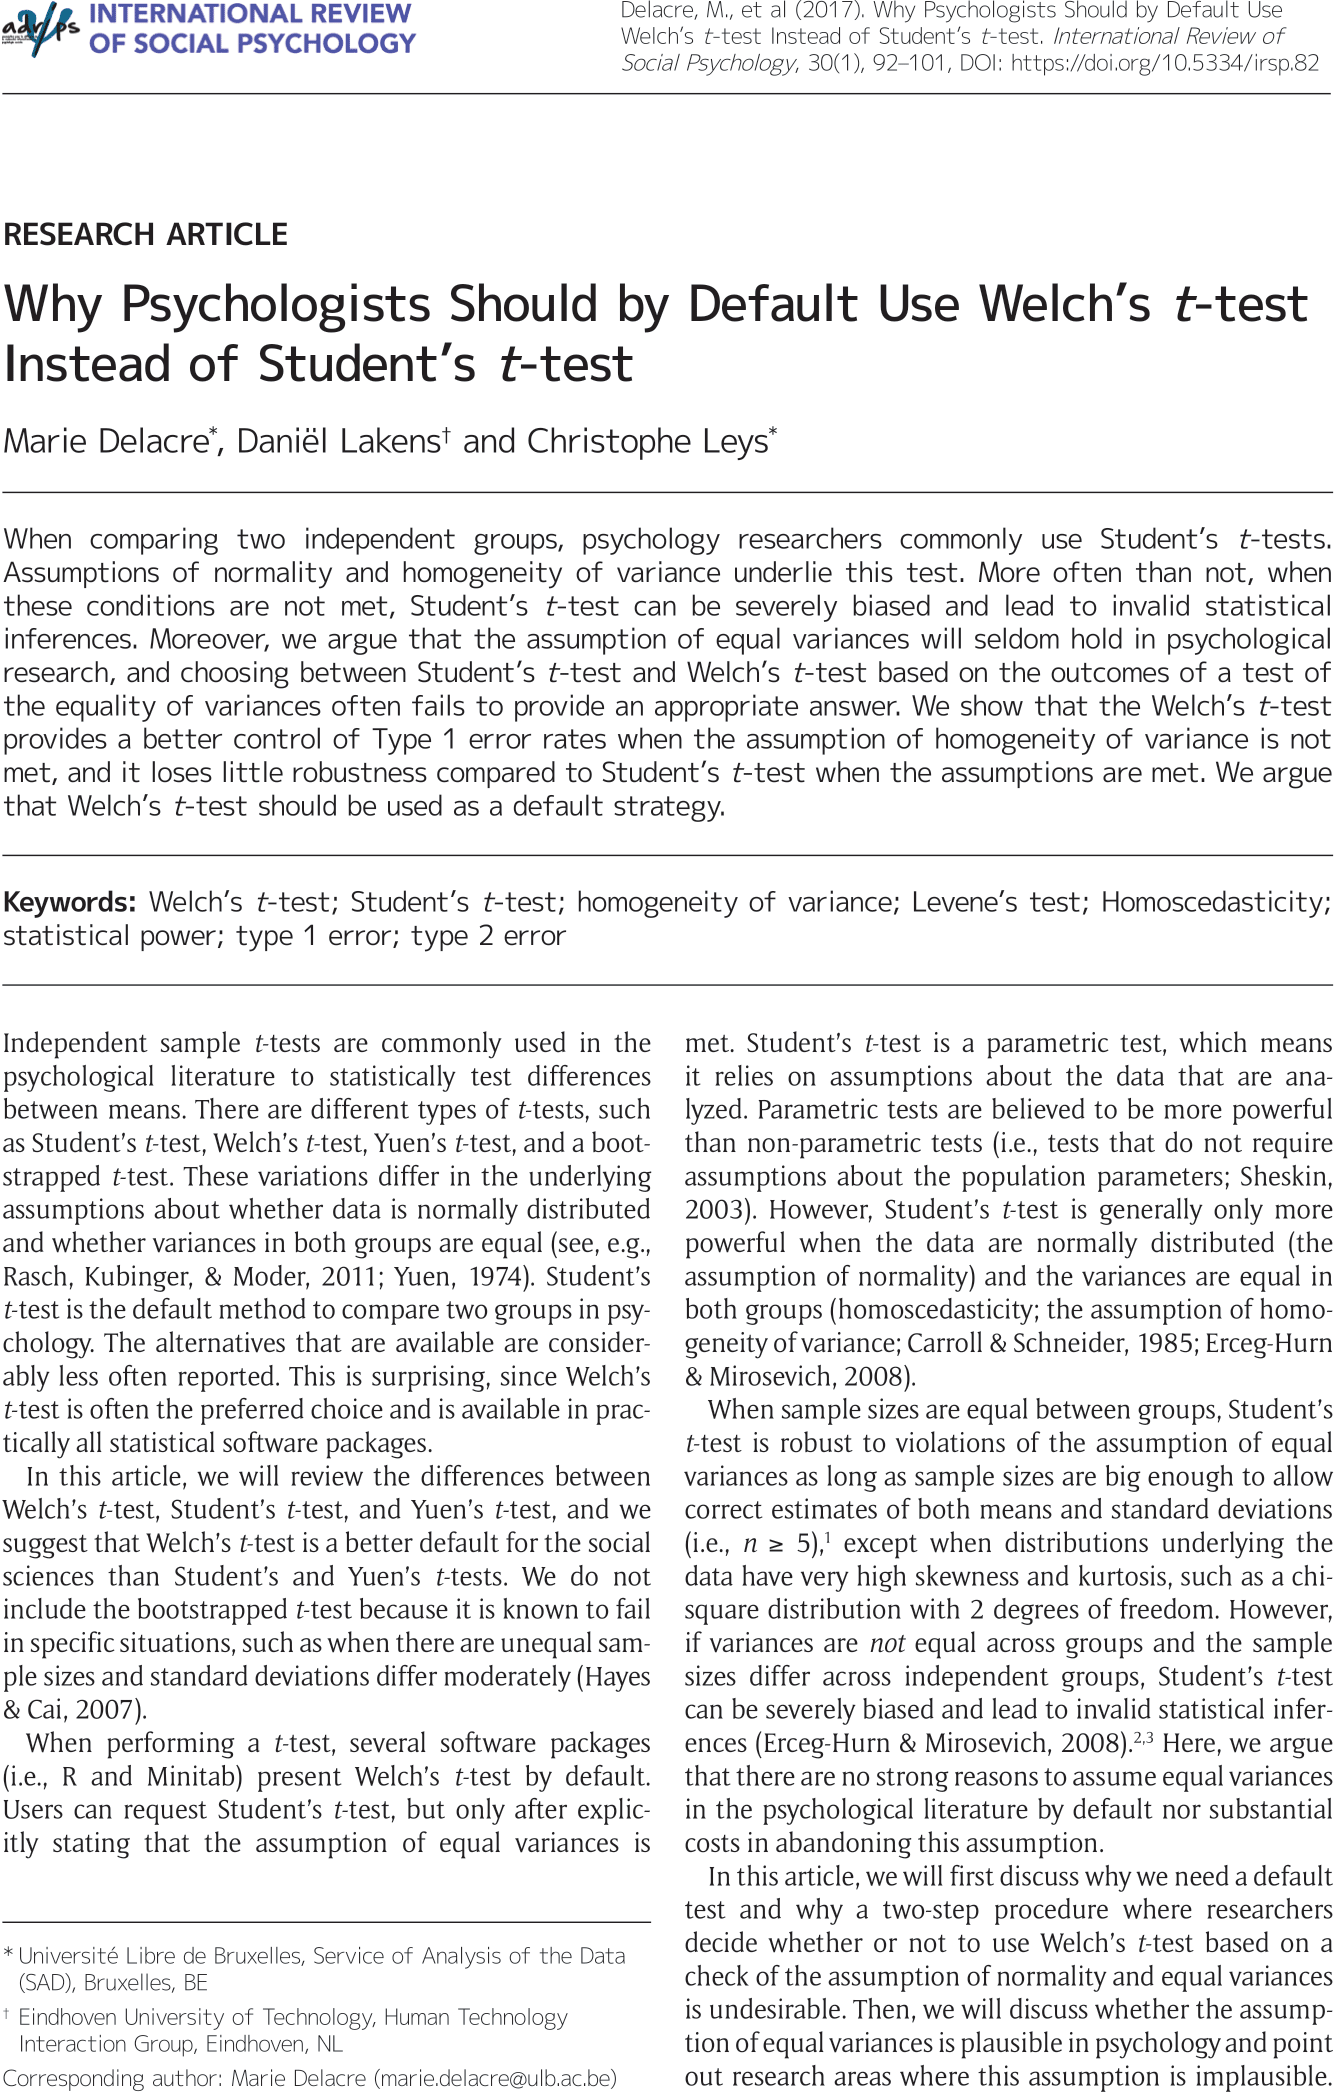
\includegraphics[width=0.92\linewidth]{C:/Users/Admin/Documents/Github projects/thesis/Chapitre 2/Chapitre 2-1} \end{center}

\begin{center}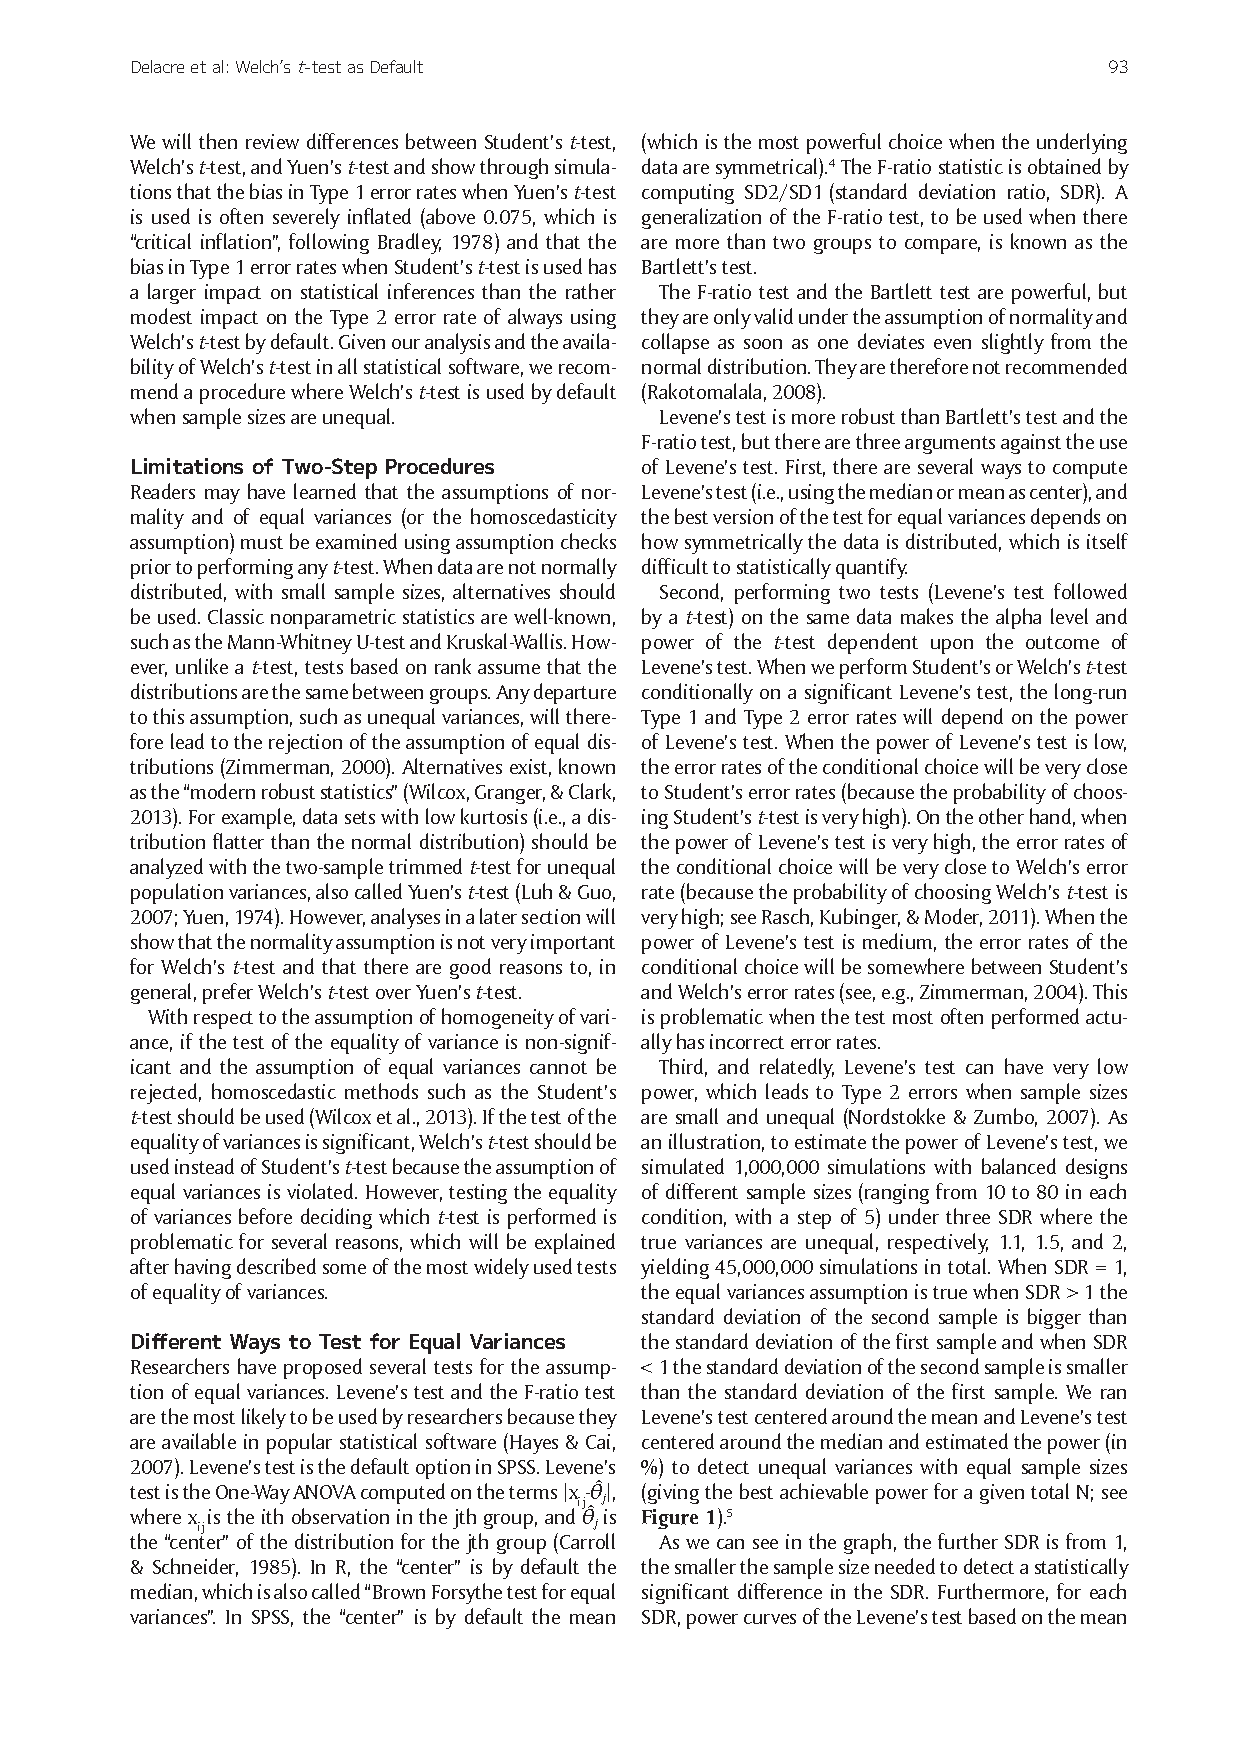
\includegraphics{C:/Users/Admin/Documents/Github projects/thesis/Chapitre 2/Chapitre 2-2} \end{center}

\begin{center}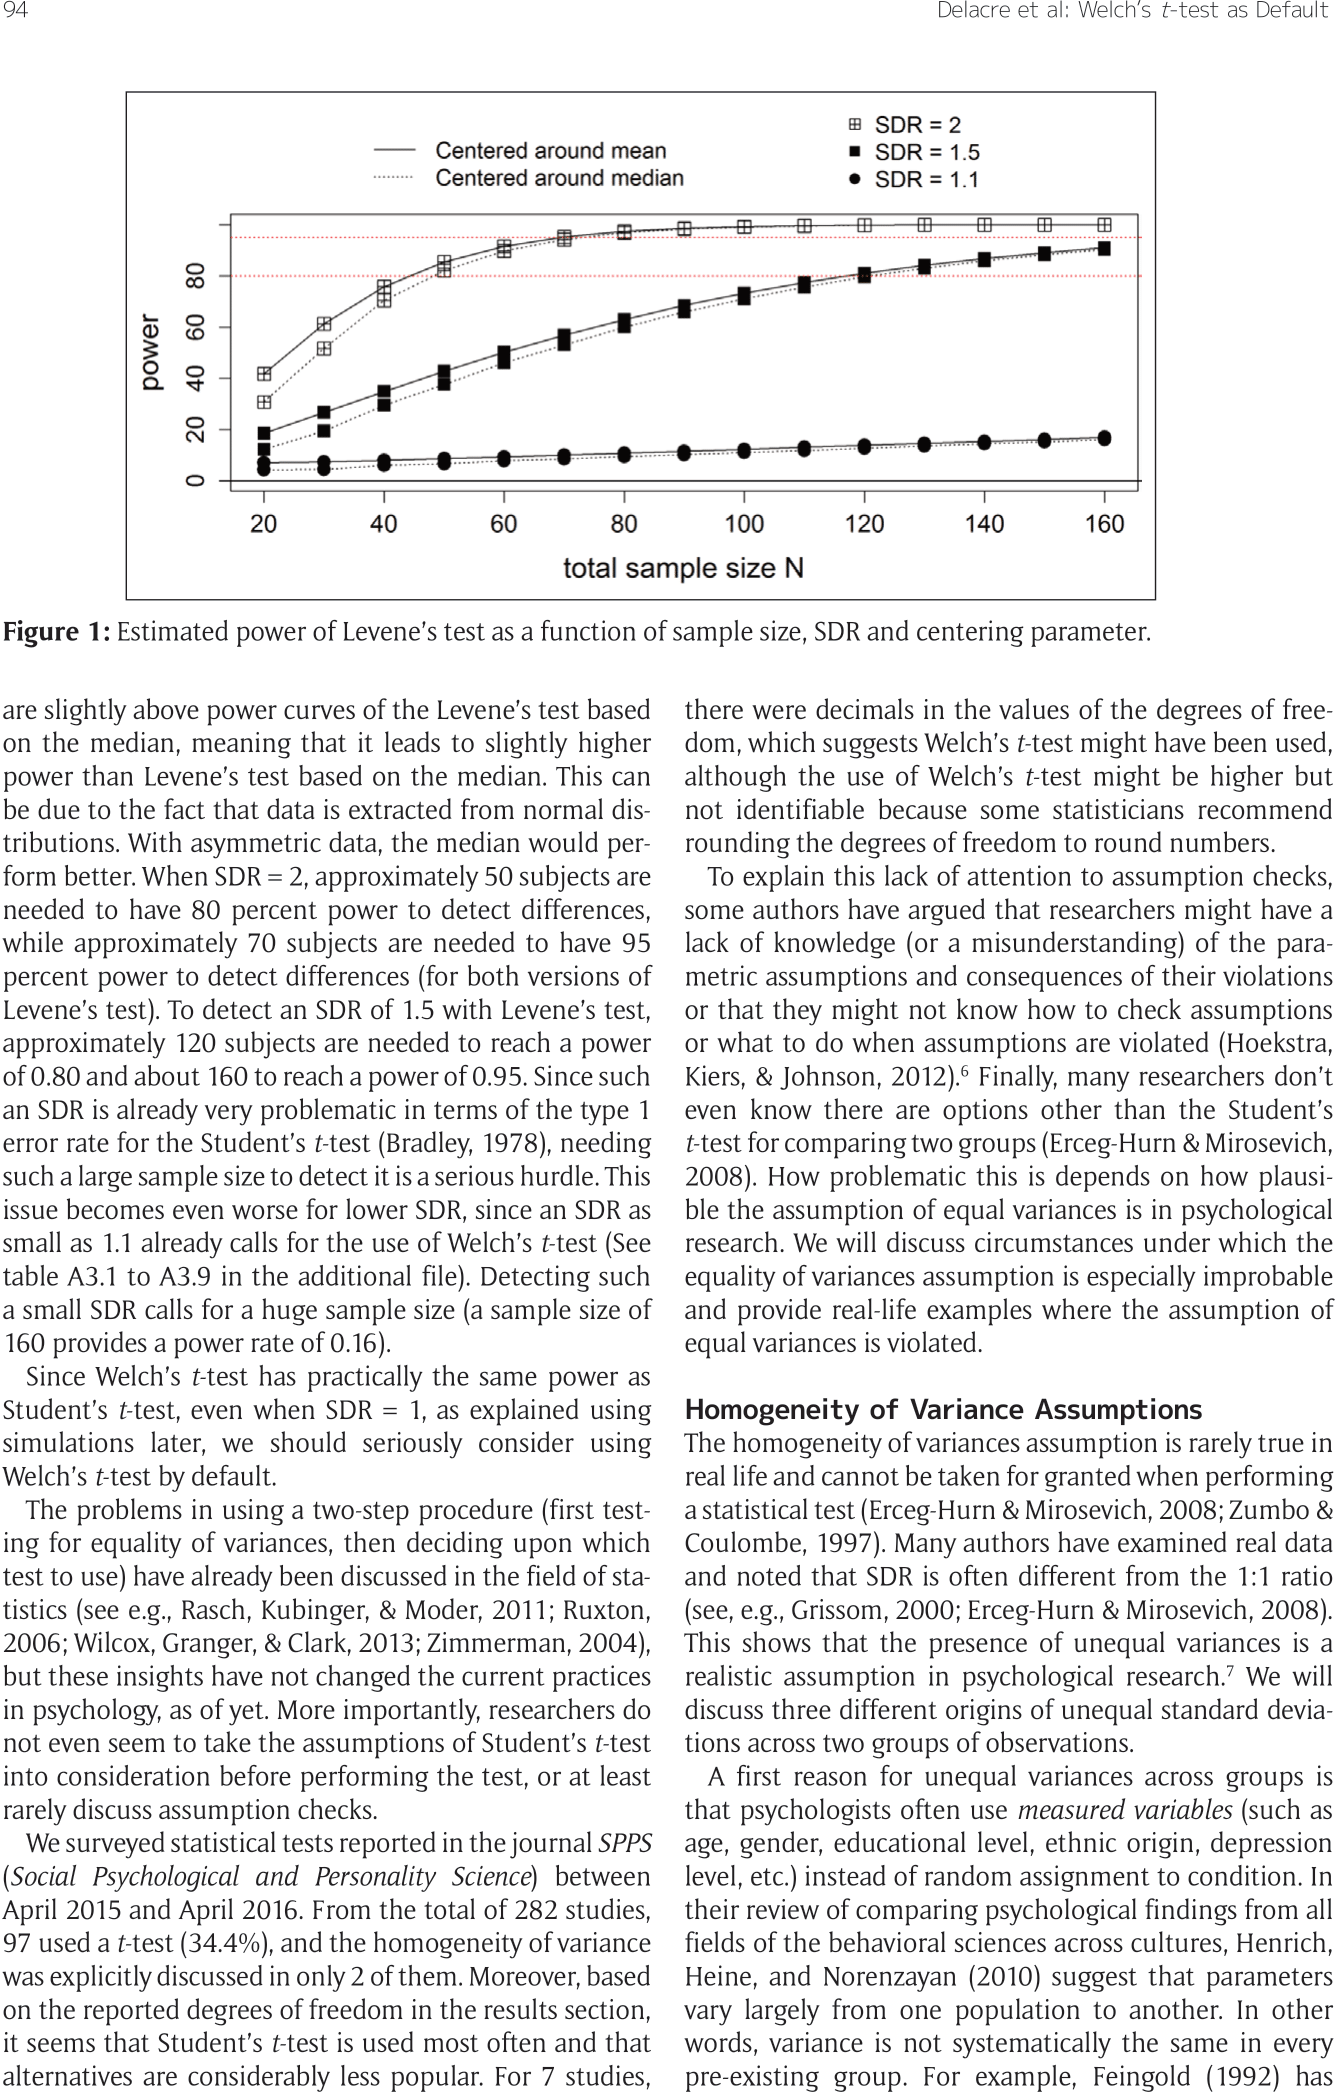
\includegraphics{C:/Users/Admin/Documents/Github projects/thesis/Chapitre 2/Chapitre 2-3} \end{center}

\begin{center}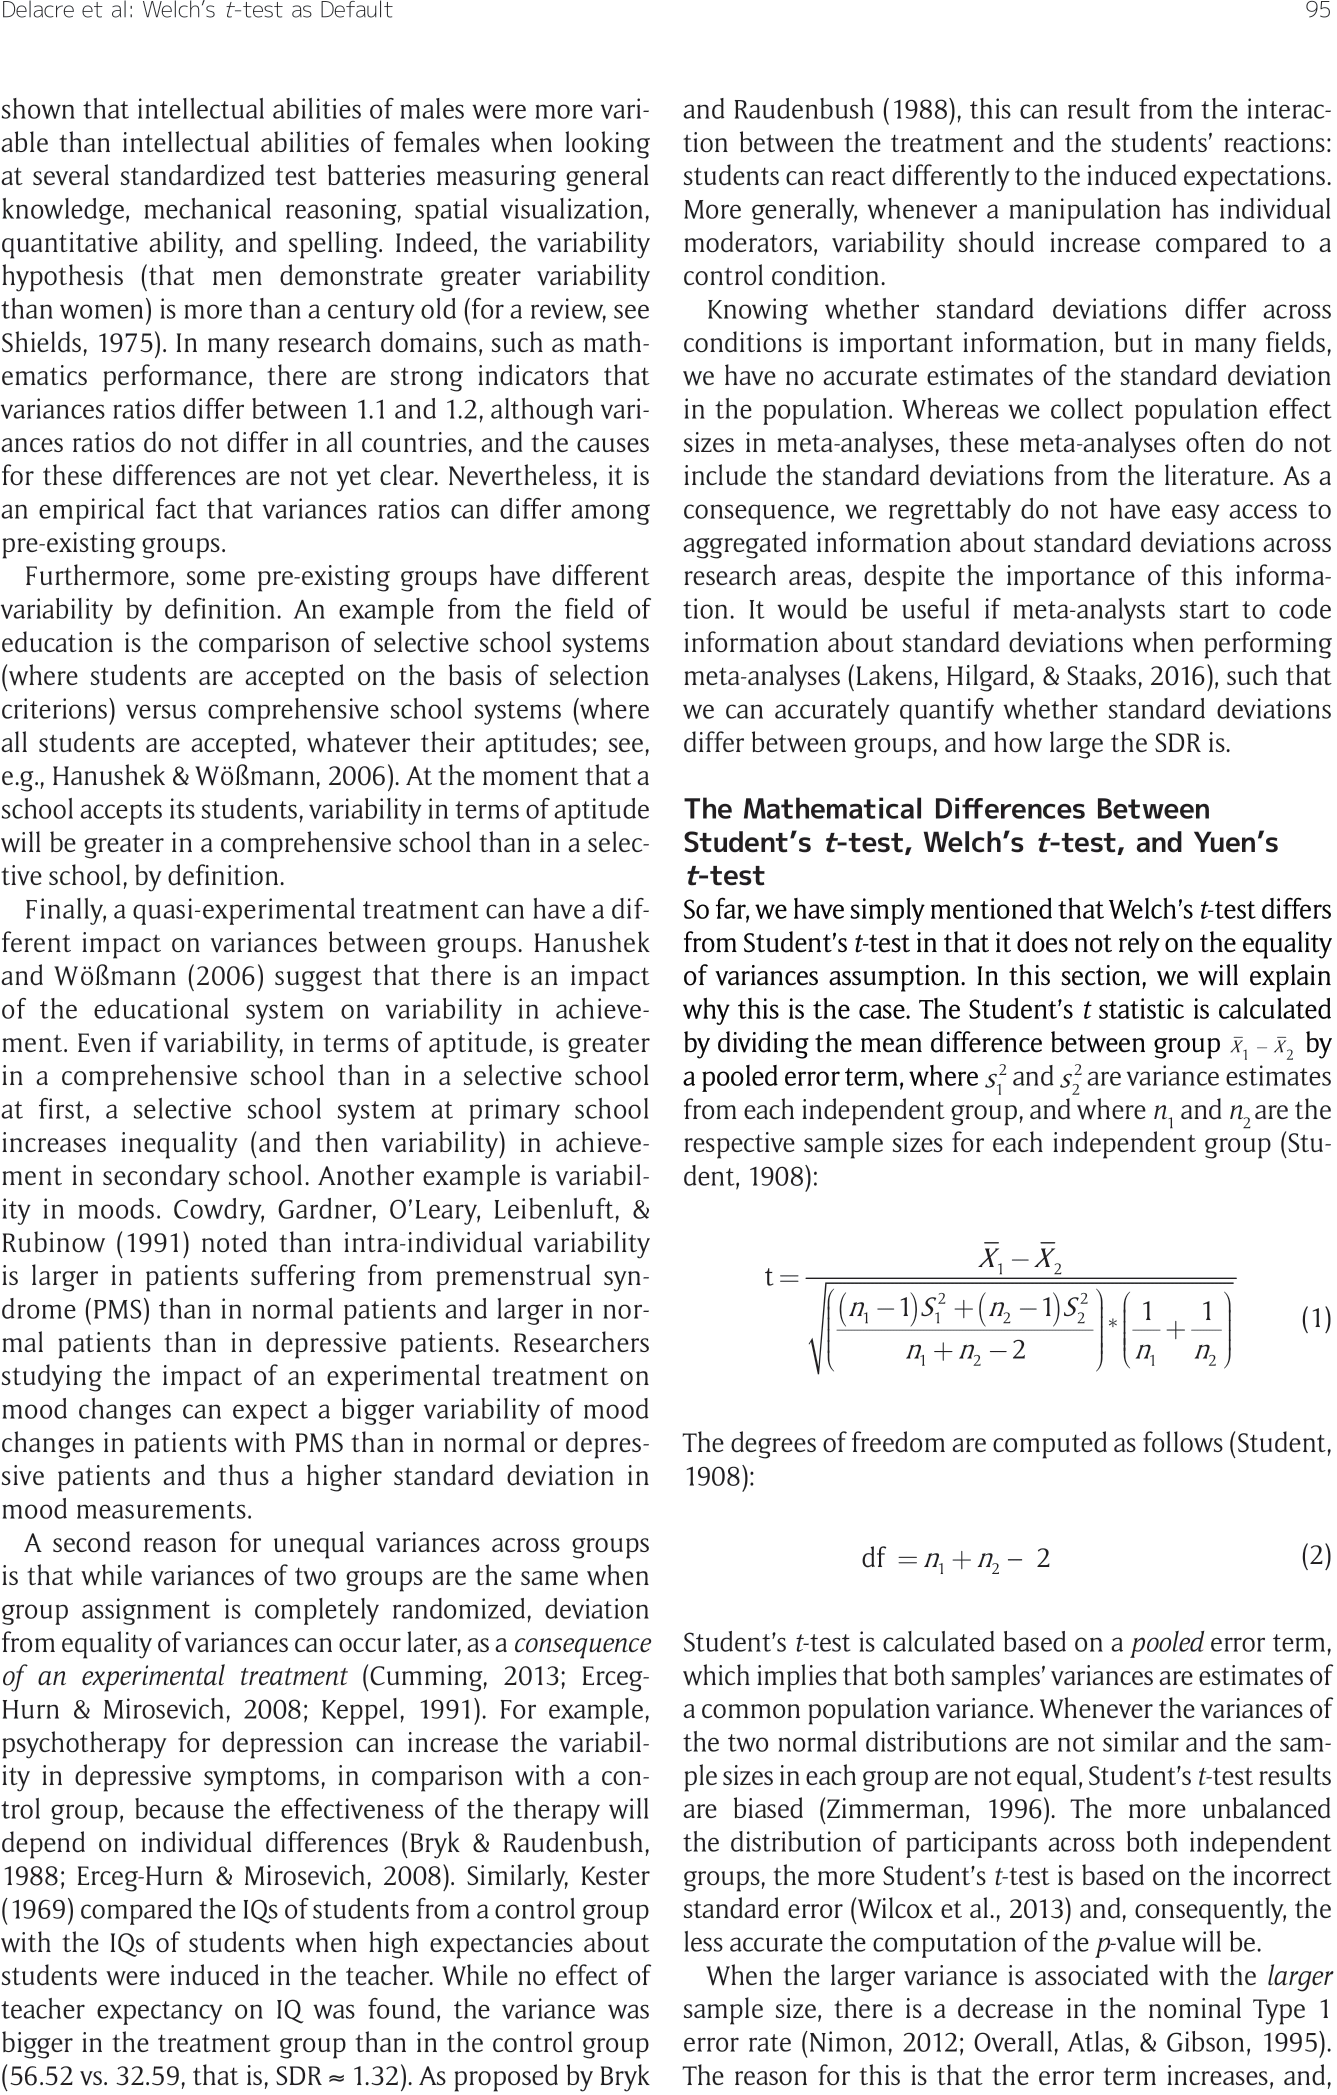
\includegraphics{C:/Users/Admin/Documents/Github projects/thesis/Chapitre 2/Chapitre 2-4} \end{center}

\begin{center}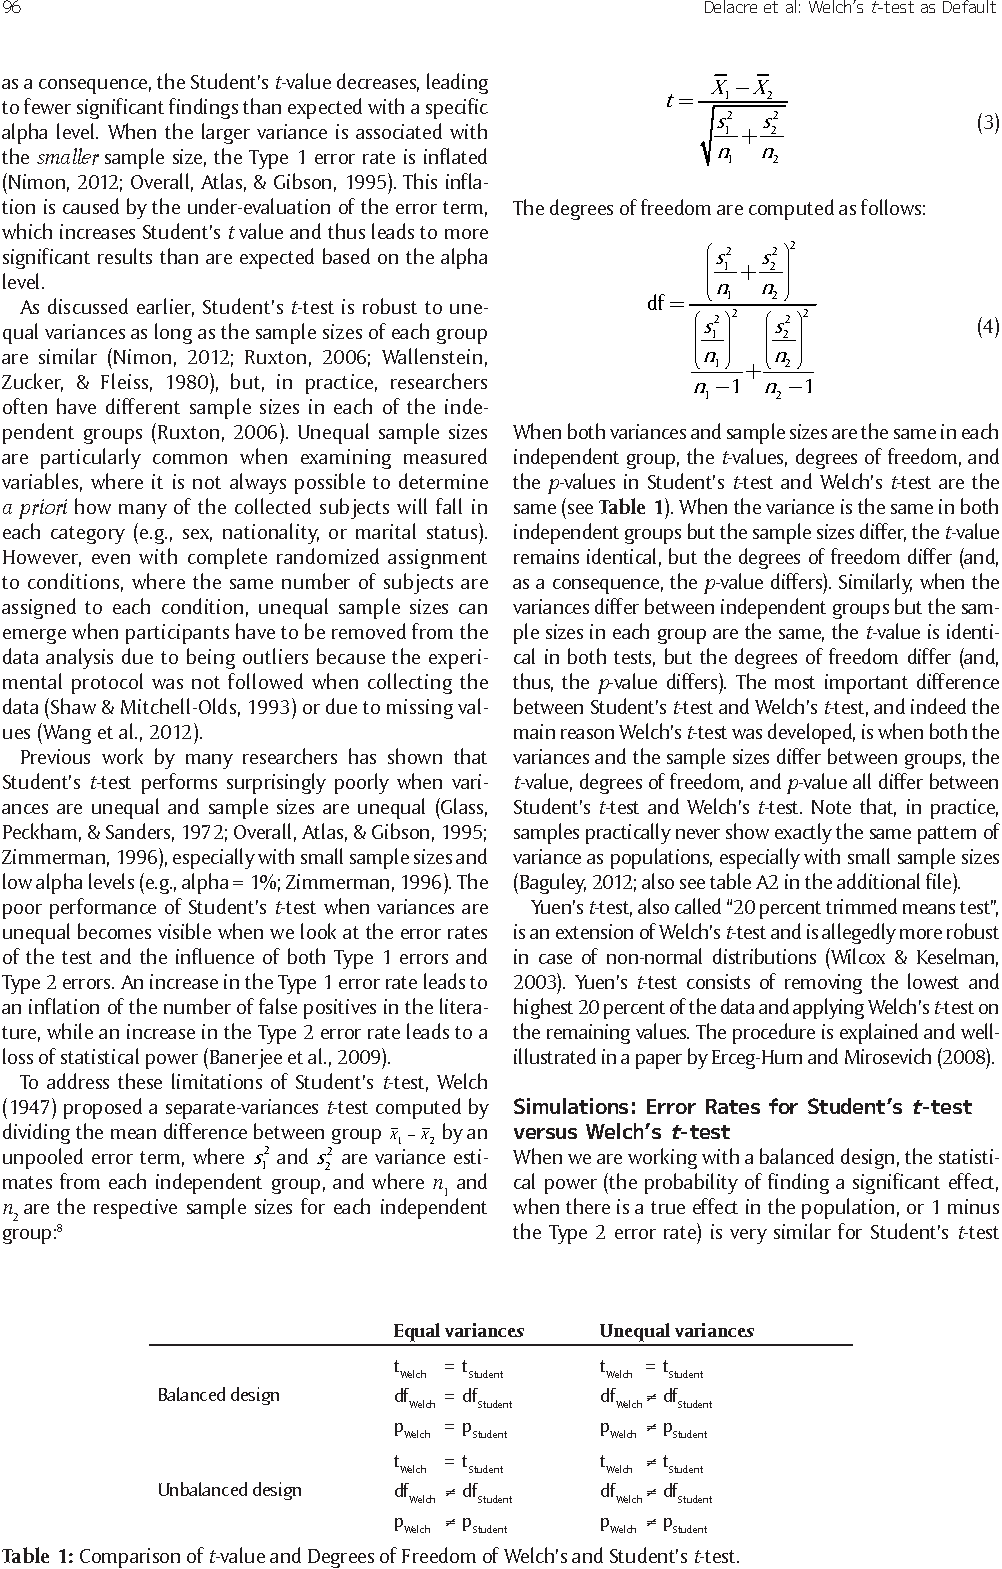
\includegraphics{C:/Users/Admin/Documents/Github projects/thesis/Chapitre 2/Chapitre 2-5} \end{center}

\begin{center}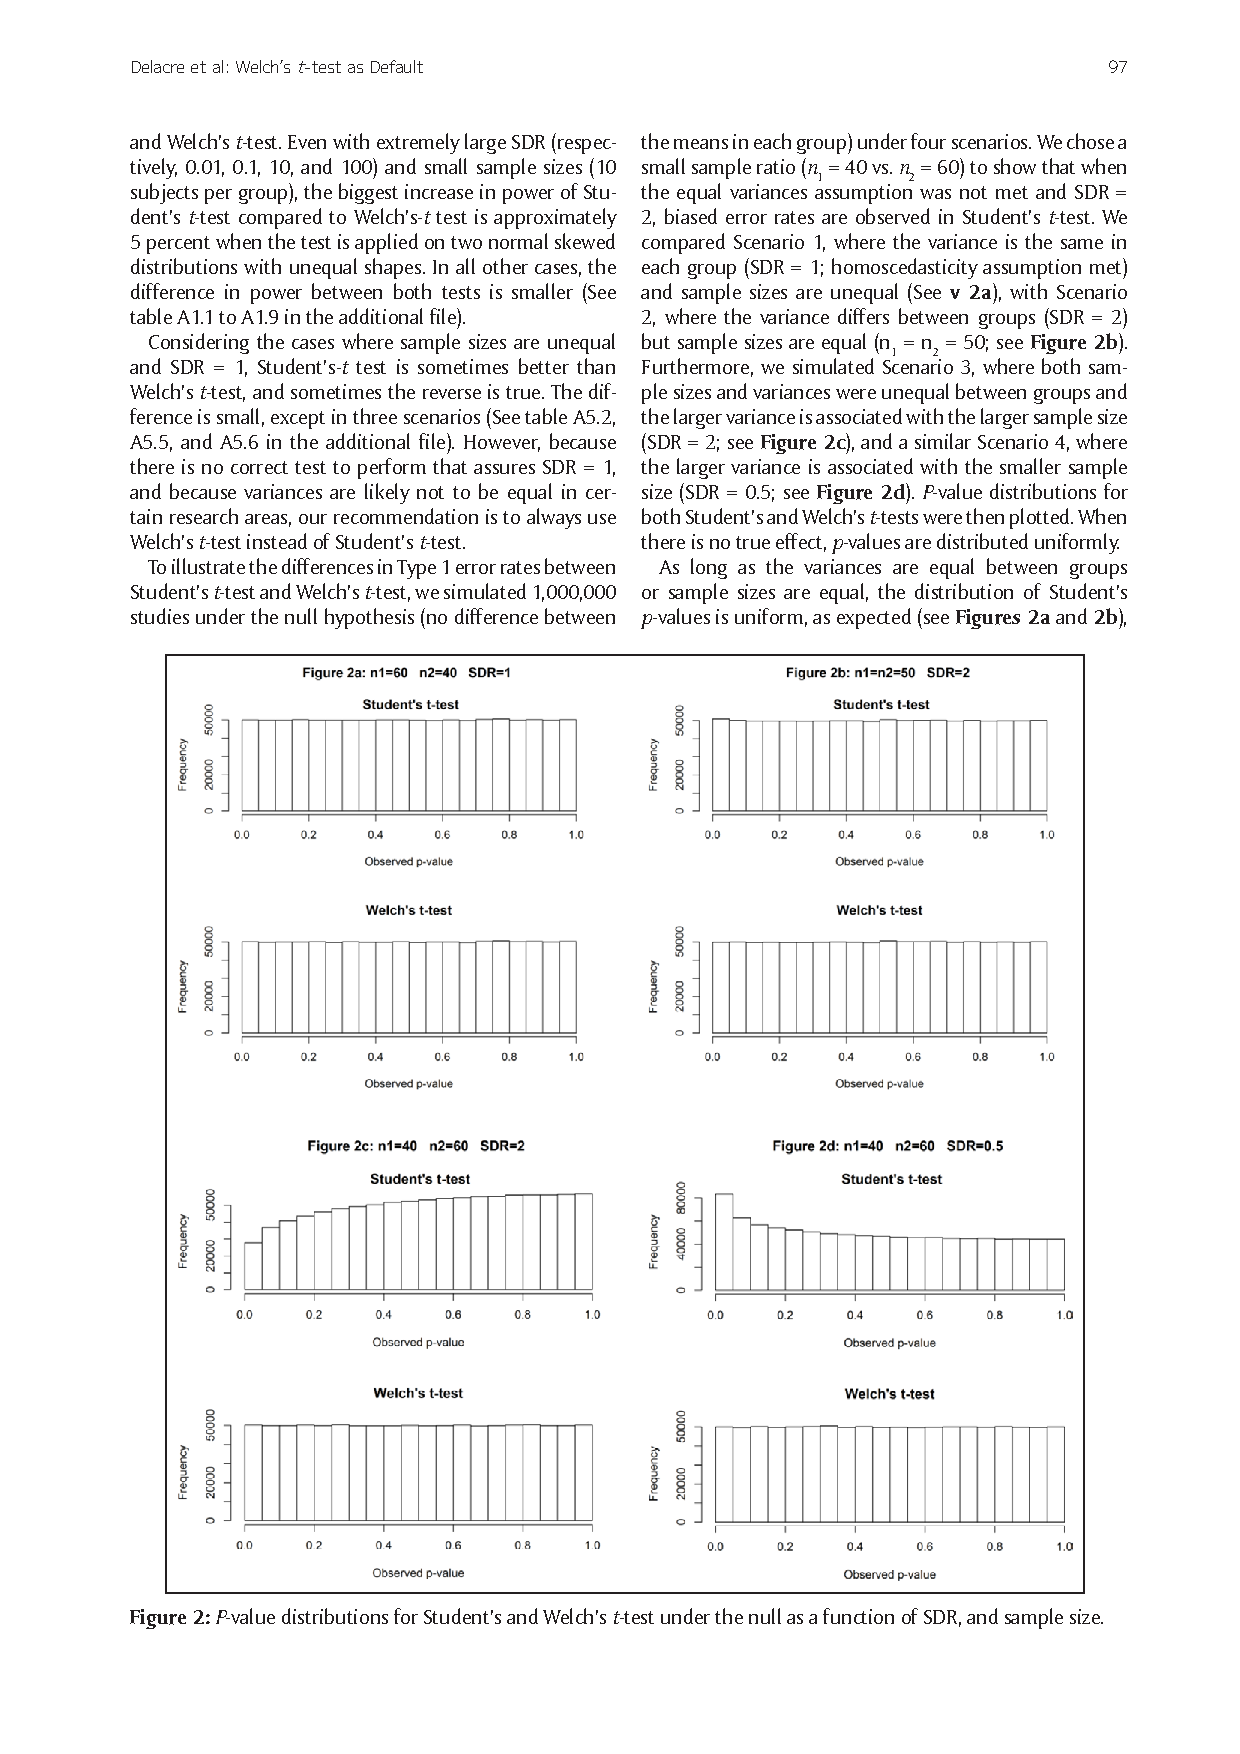
\includegraphics{C:/Users/Admin/Documents/Github projects/thesis/Chapitre 2/Chapitre 2-6} \end{center}

\begin{center}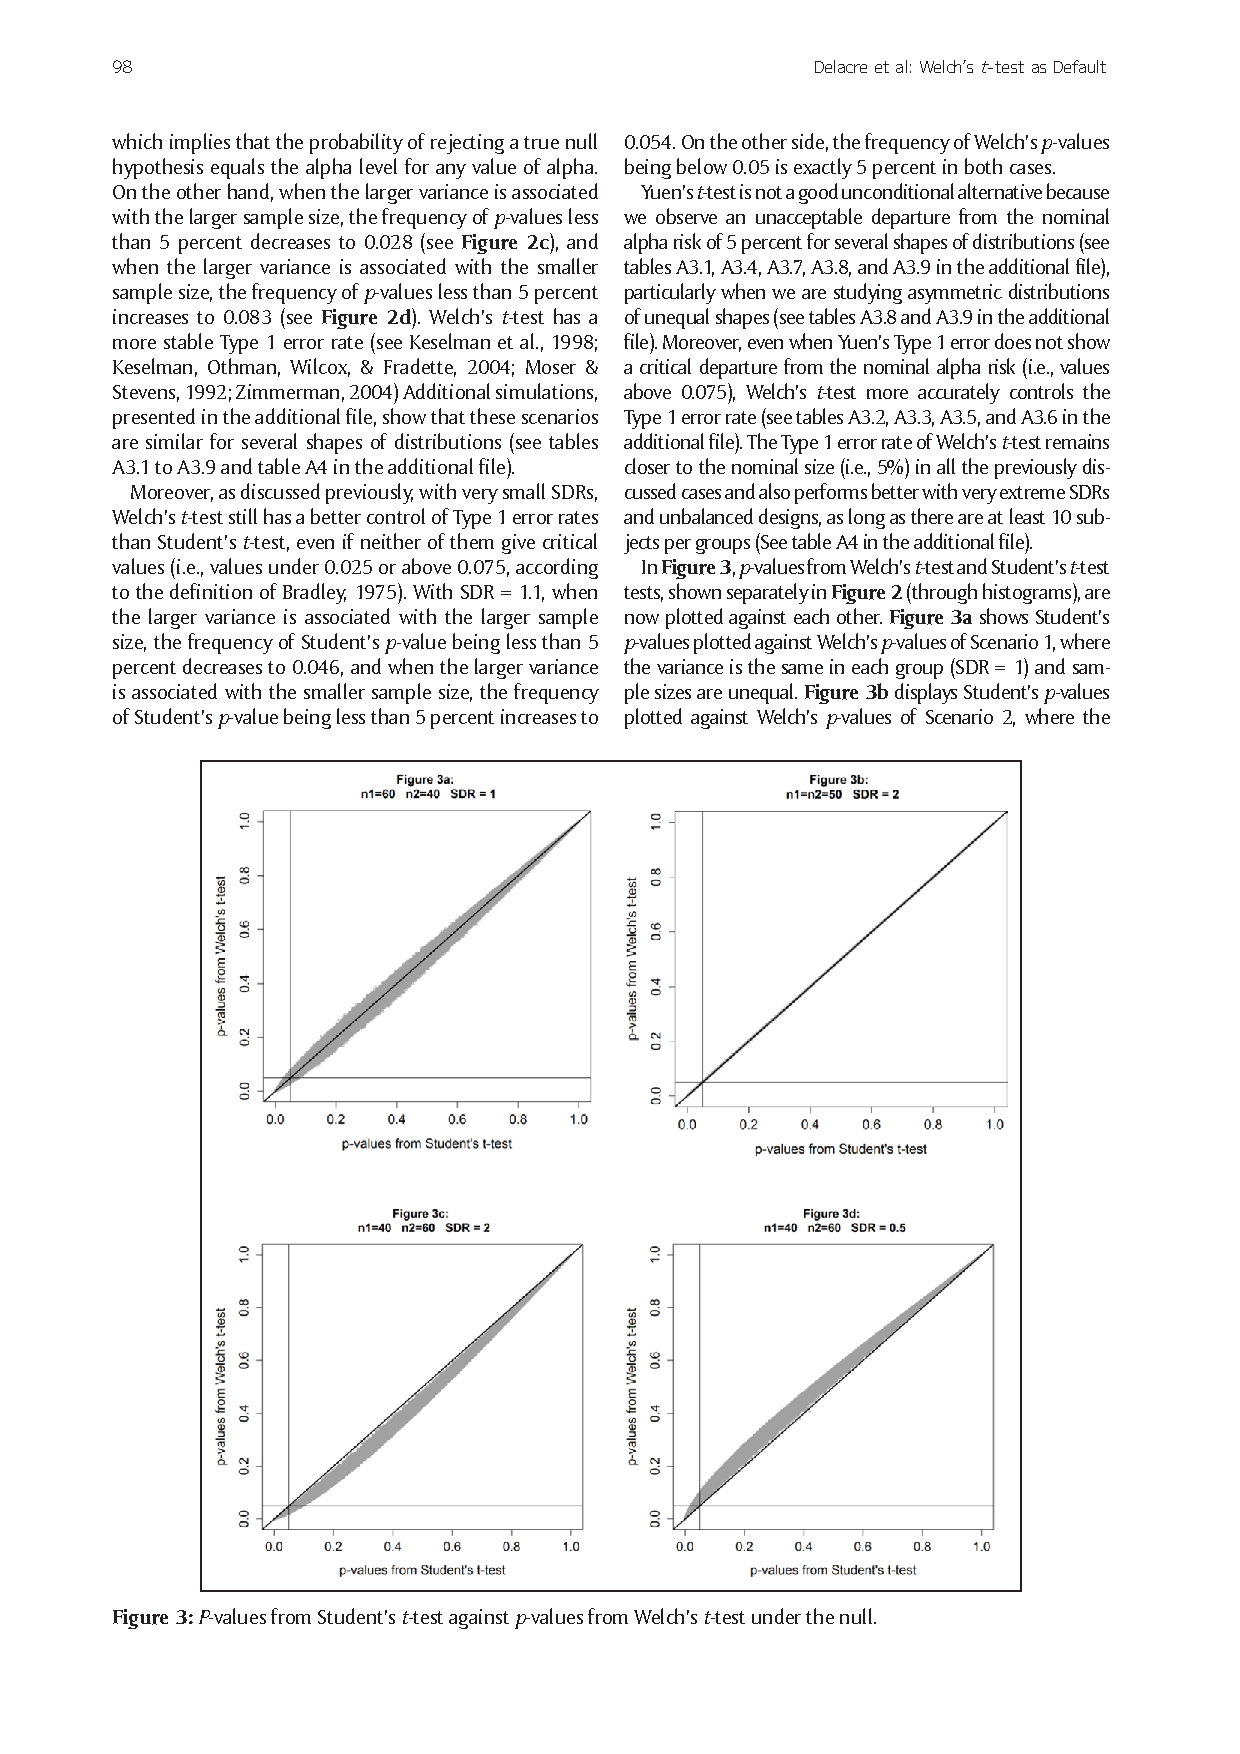
\includegraphics{C:/Users/Admin/Documents/Github projects/thesis/Chapitre 2/Chapitre 2-7} \end{center}

\begin{center}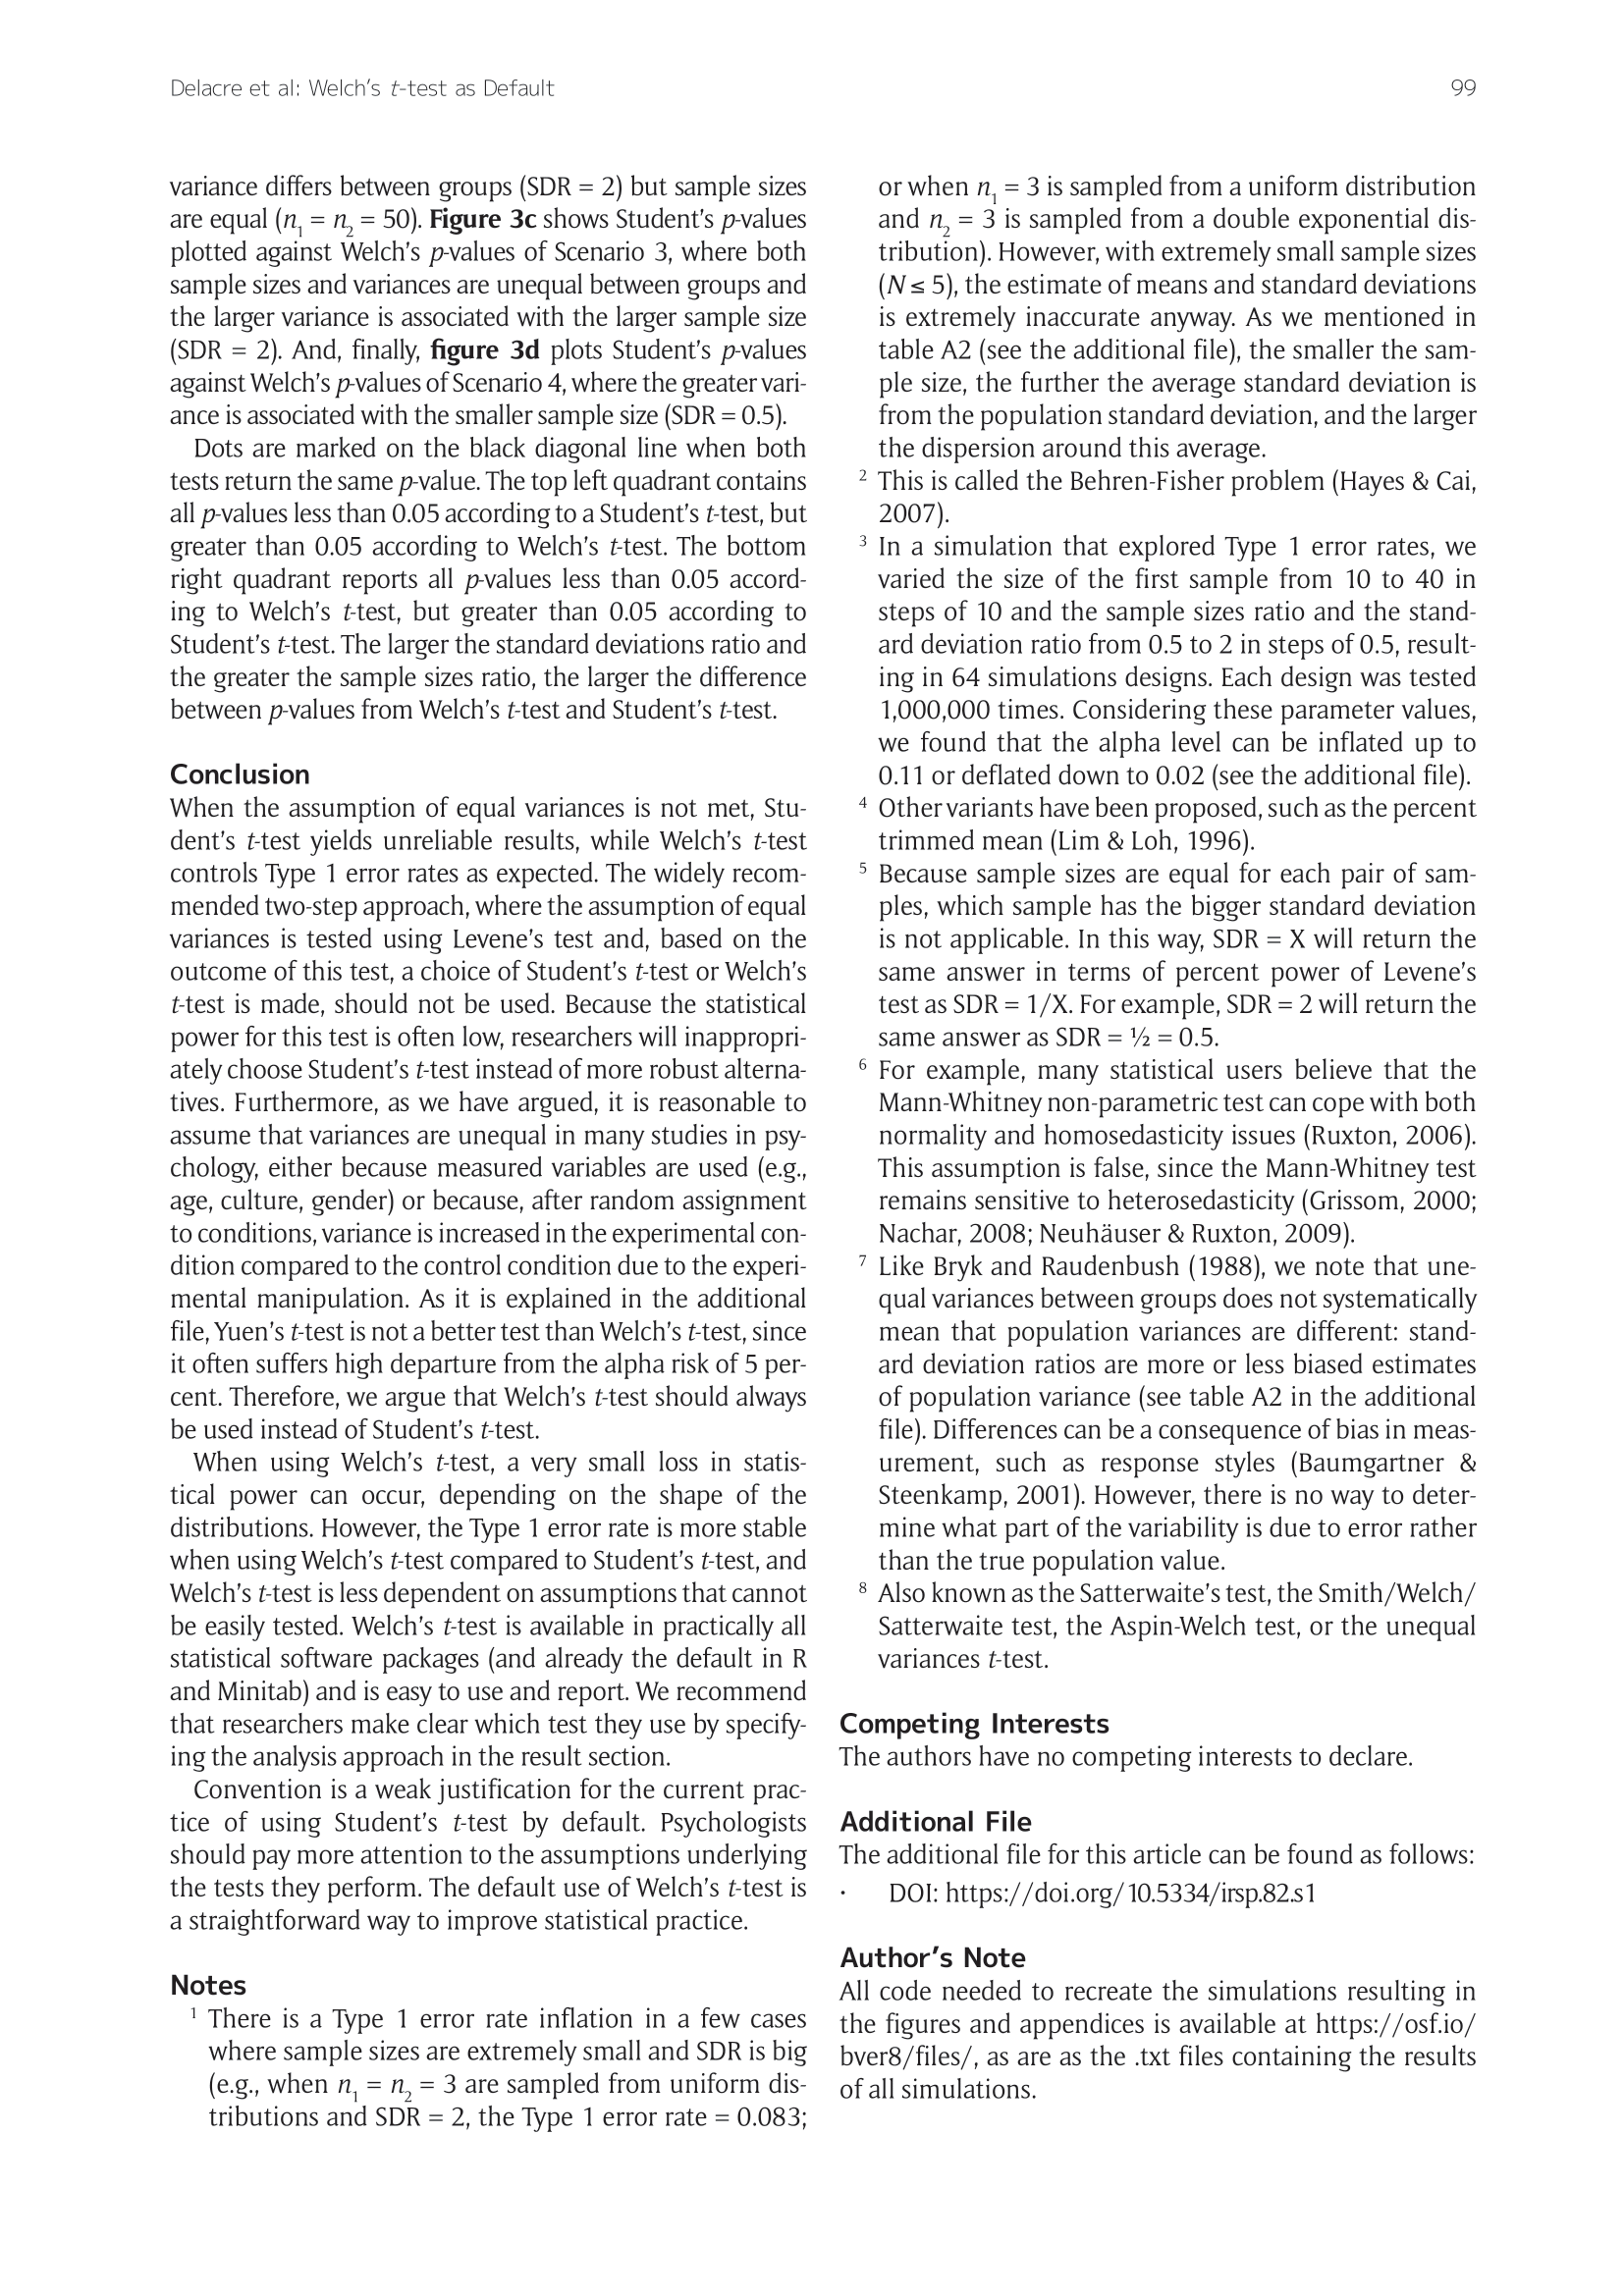
\includegraphics{C:/Users/Admin/Documents/Github projects/thesis/Chapitre 2/Chapitre 2-8} \end{center}

\begin{center}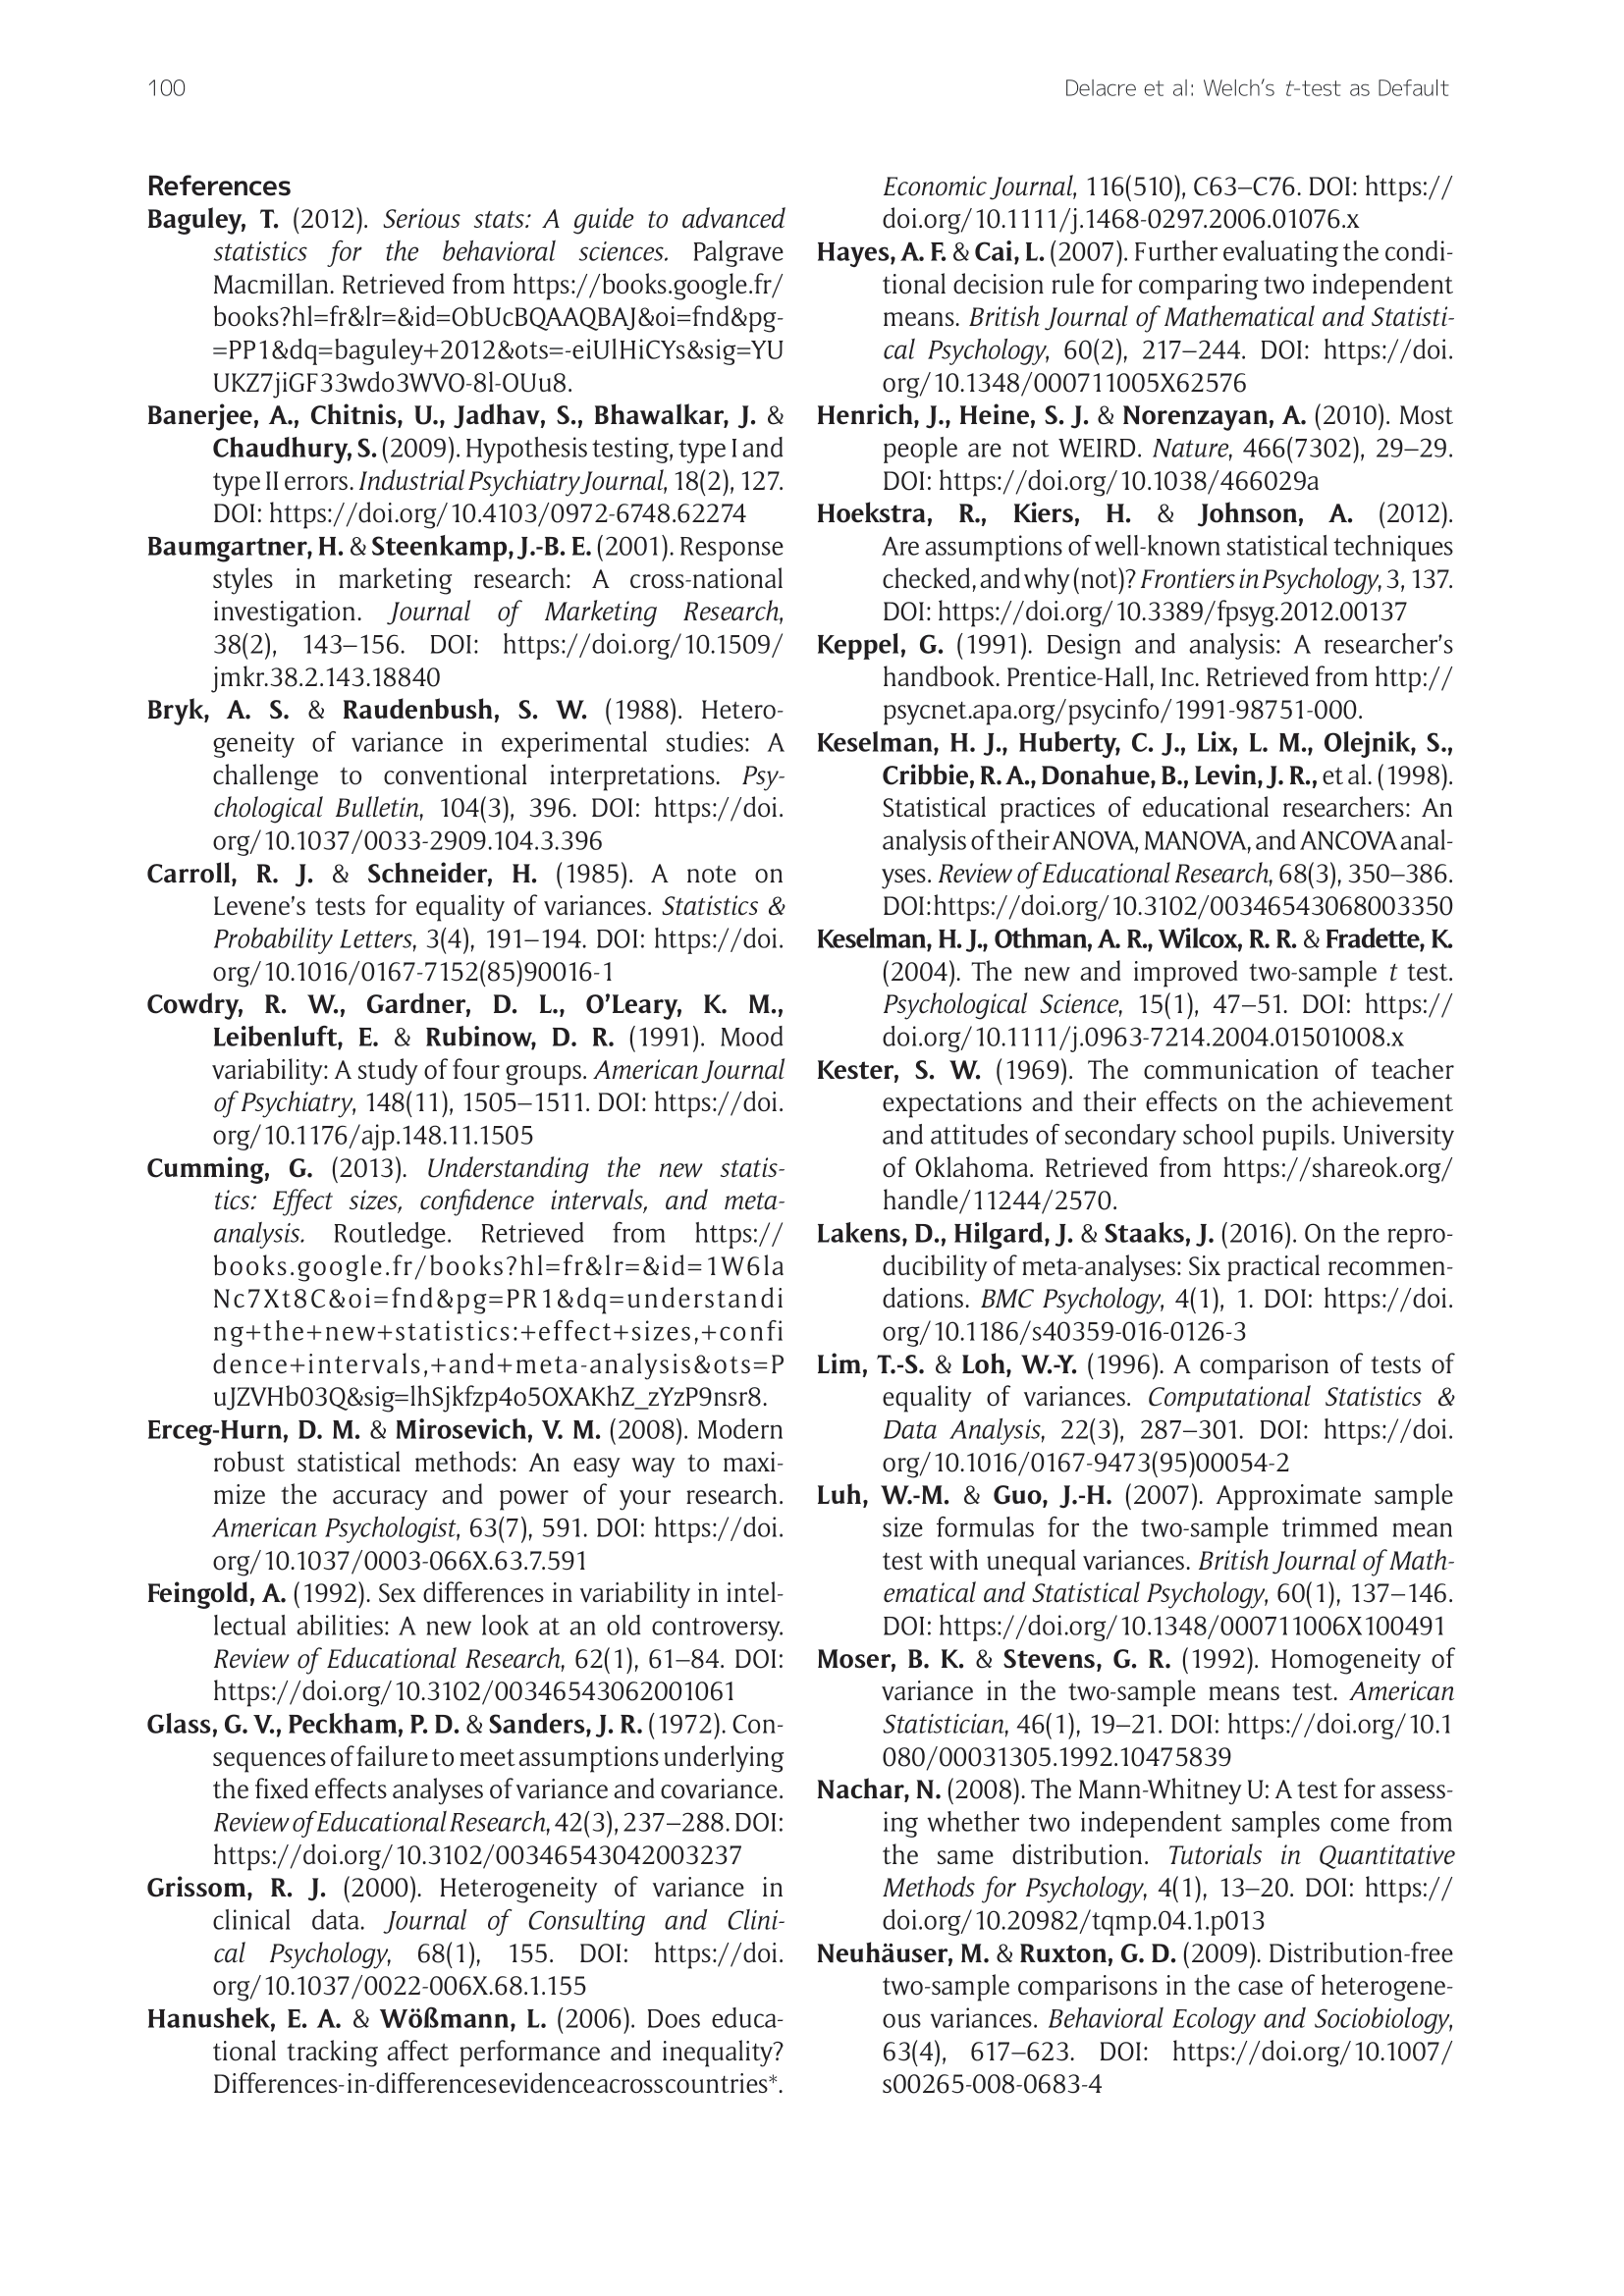
\includegraphics{C:/Users/Admin/Documents/Github projects/thesis/Chapitre 2/Chapitre 2-9} \end{center}

\begin{center}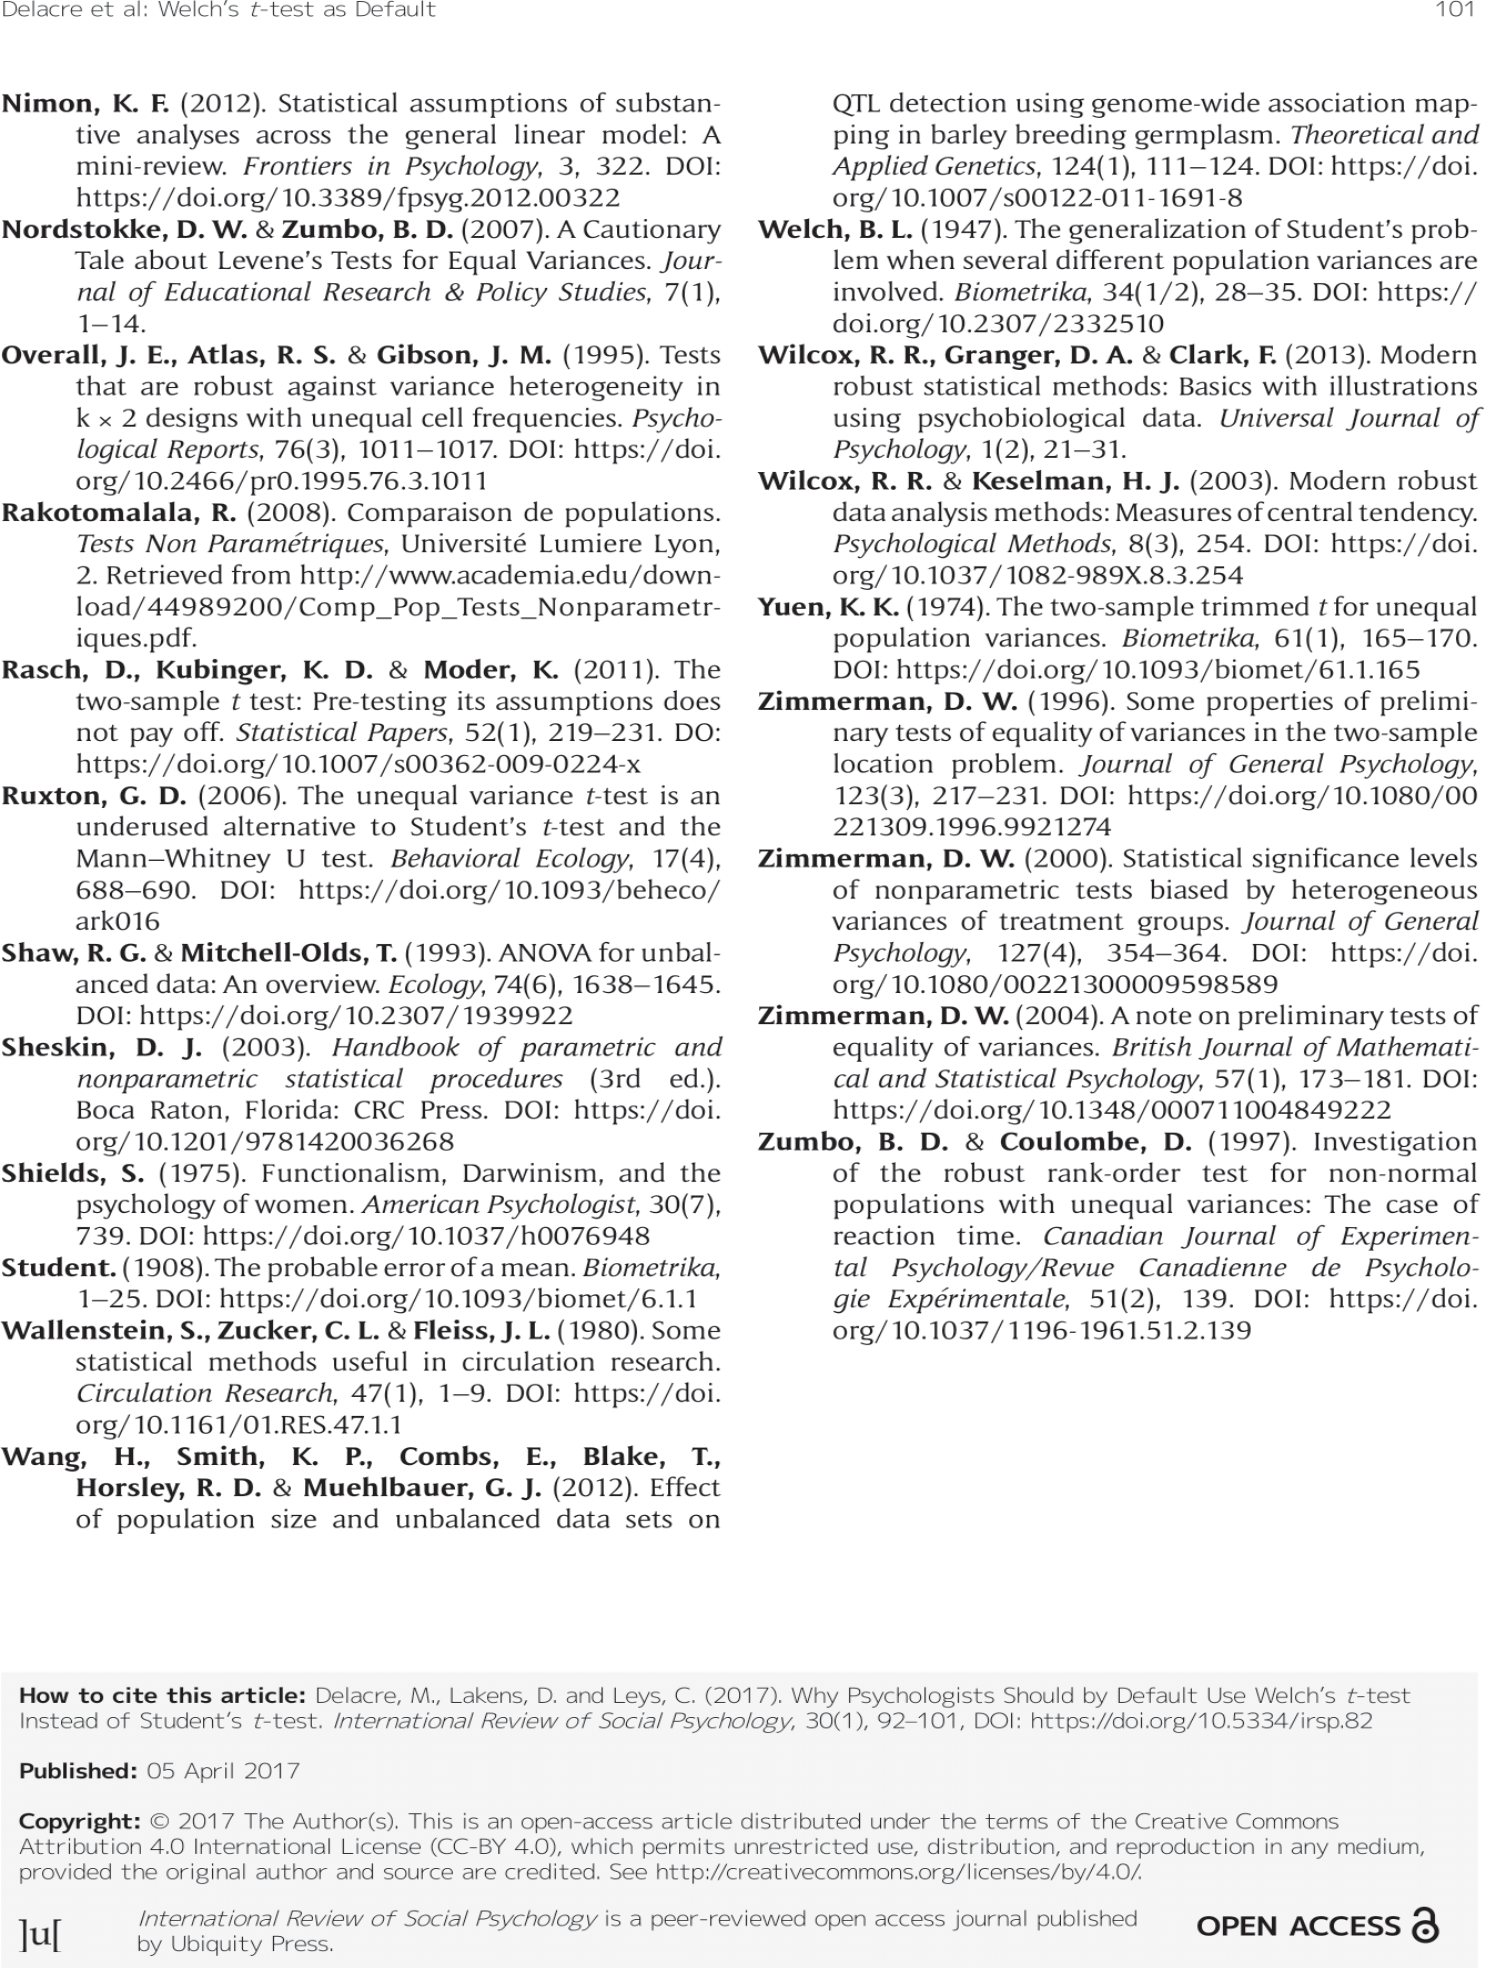
\includegraphics[width=0.82\linewidth]{C:/Users/Admin/Documents/Github projects/thesis/Chapitre 2/Chapitre 2-10} \end{center}

\begingroup
\parindent 0pt
\renewcommand\notesname{{\normalsize Note de fin de chapitre}}

\parskip 1ex \theendnotes \endgroup

\newpage

\hypertarget{chapitre-3-utiliser-lanova-bf-emph-f-de-welch-par-duxe9faut}{%
\section[Chapitre 3: Utiliser l'ANOVA \(\bf \emph F\) de Welch par
défaut]{\texorpdfstring{Chapitre 3: Utiliser l'ANOVA \(\bf \emph F\) de
Welch par
défaut\footnote{Un erratum de cet article figure dans l'annexe B.}}{Chapitre 3: Utiliser l'ANOVA \textbackslash bf \textbackslash emph F de Welch par défaut}}\label{chapitre-3-utiliser-lanova-bf-emph-f-de-welch-par-duxe9faut}}

\begin{center}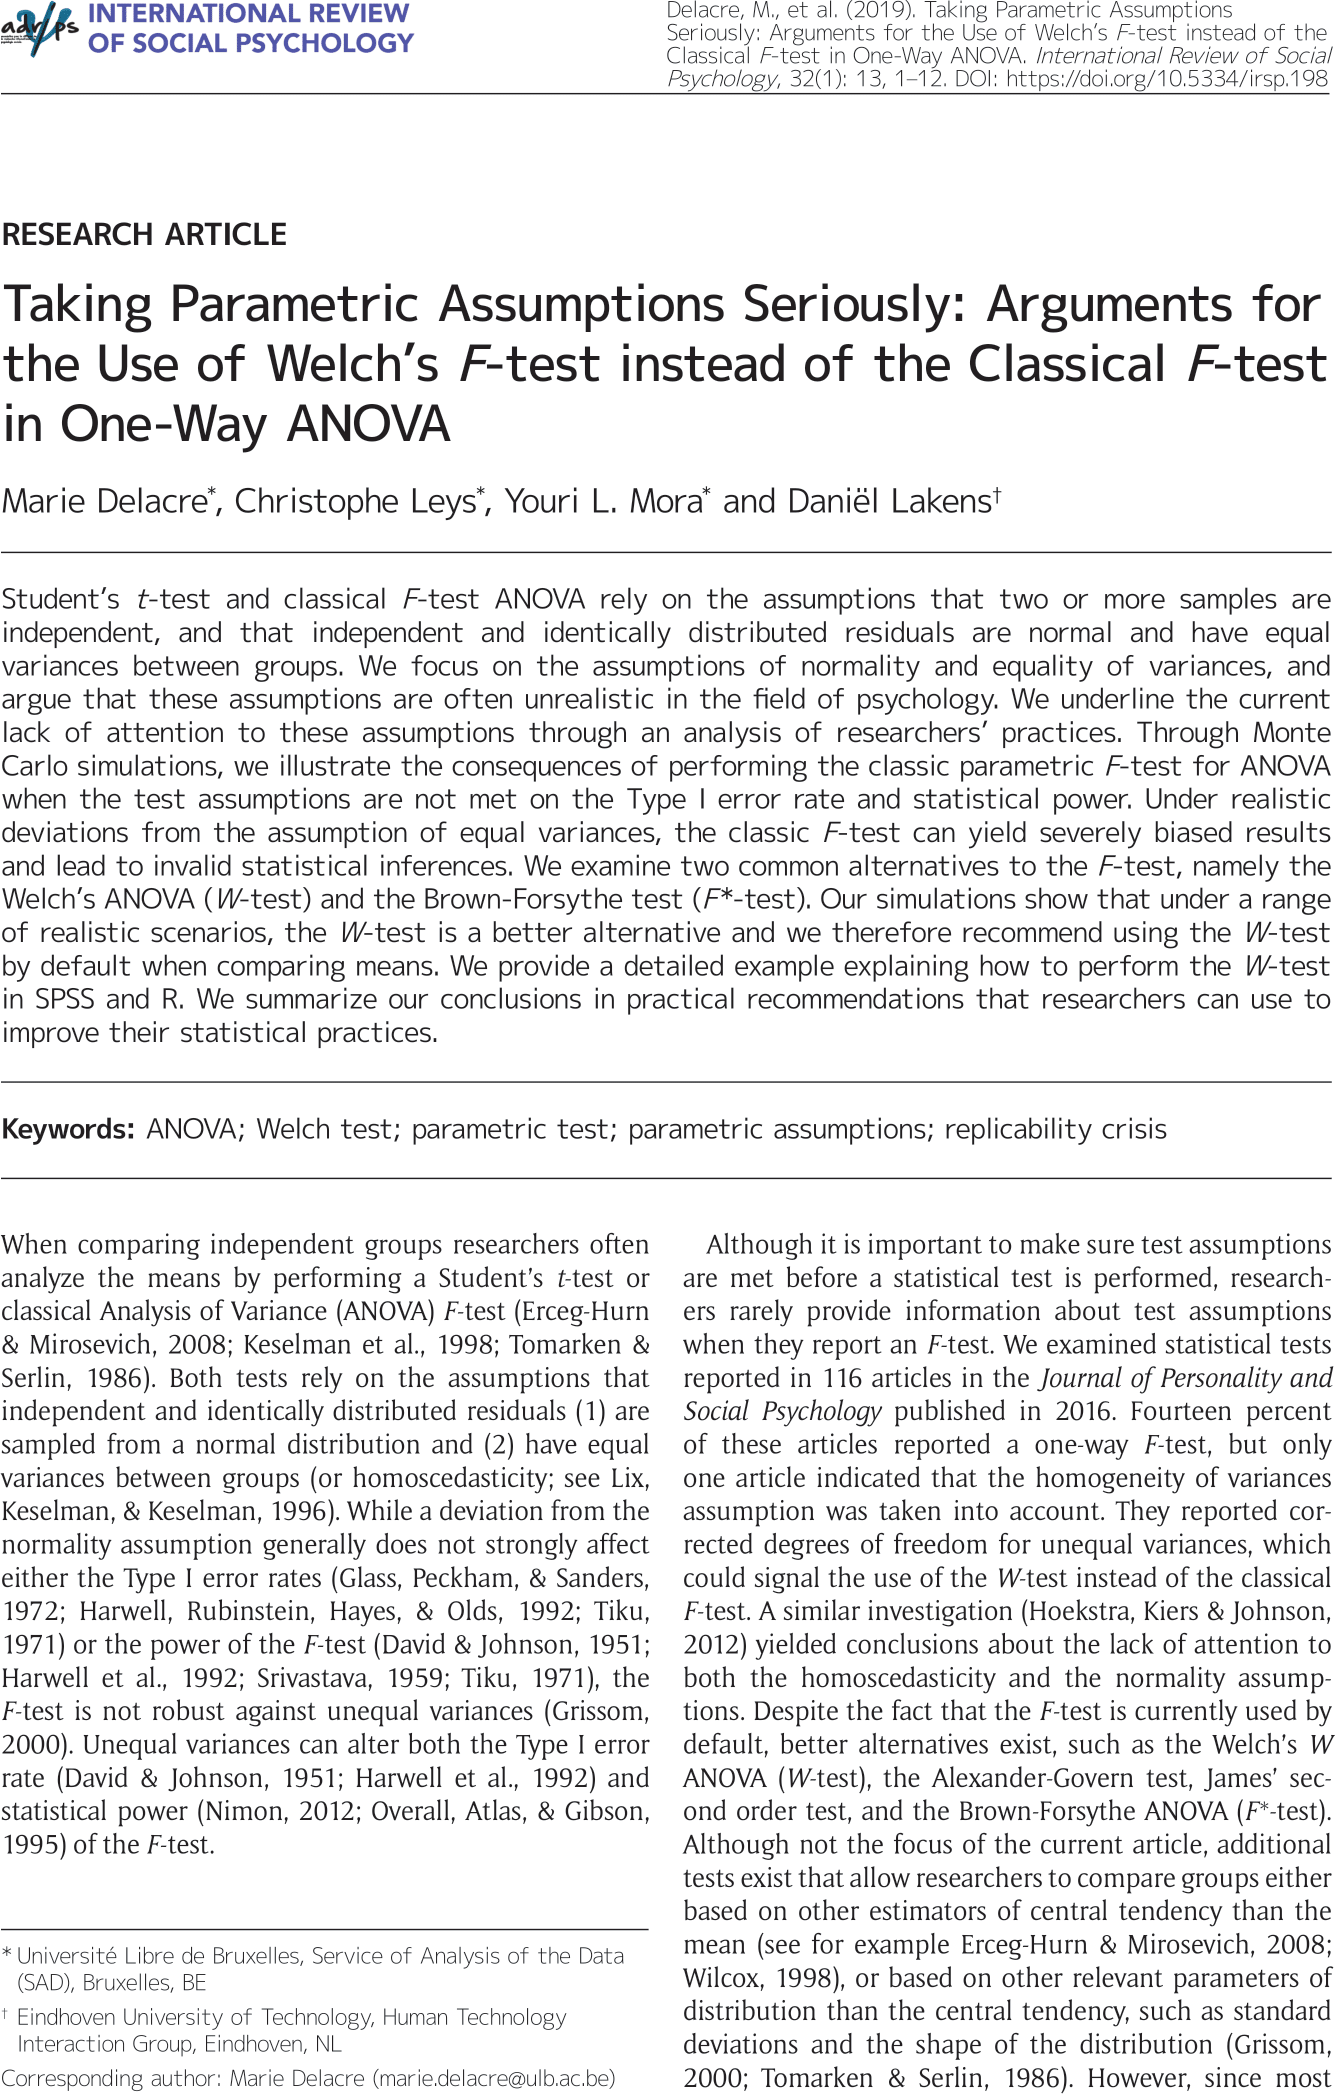
\includegraphics[width=0.92\linewidth]{C:/Users/Admin/Documents/Github projects/thesis/Chapitre 3/Chapitre 3-1} \end{center}

\begin{center}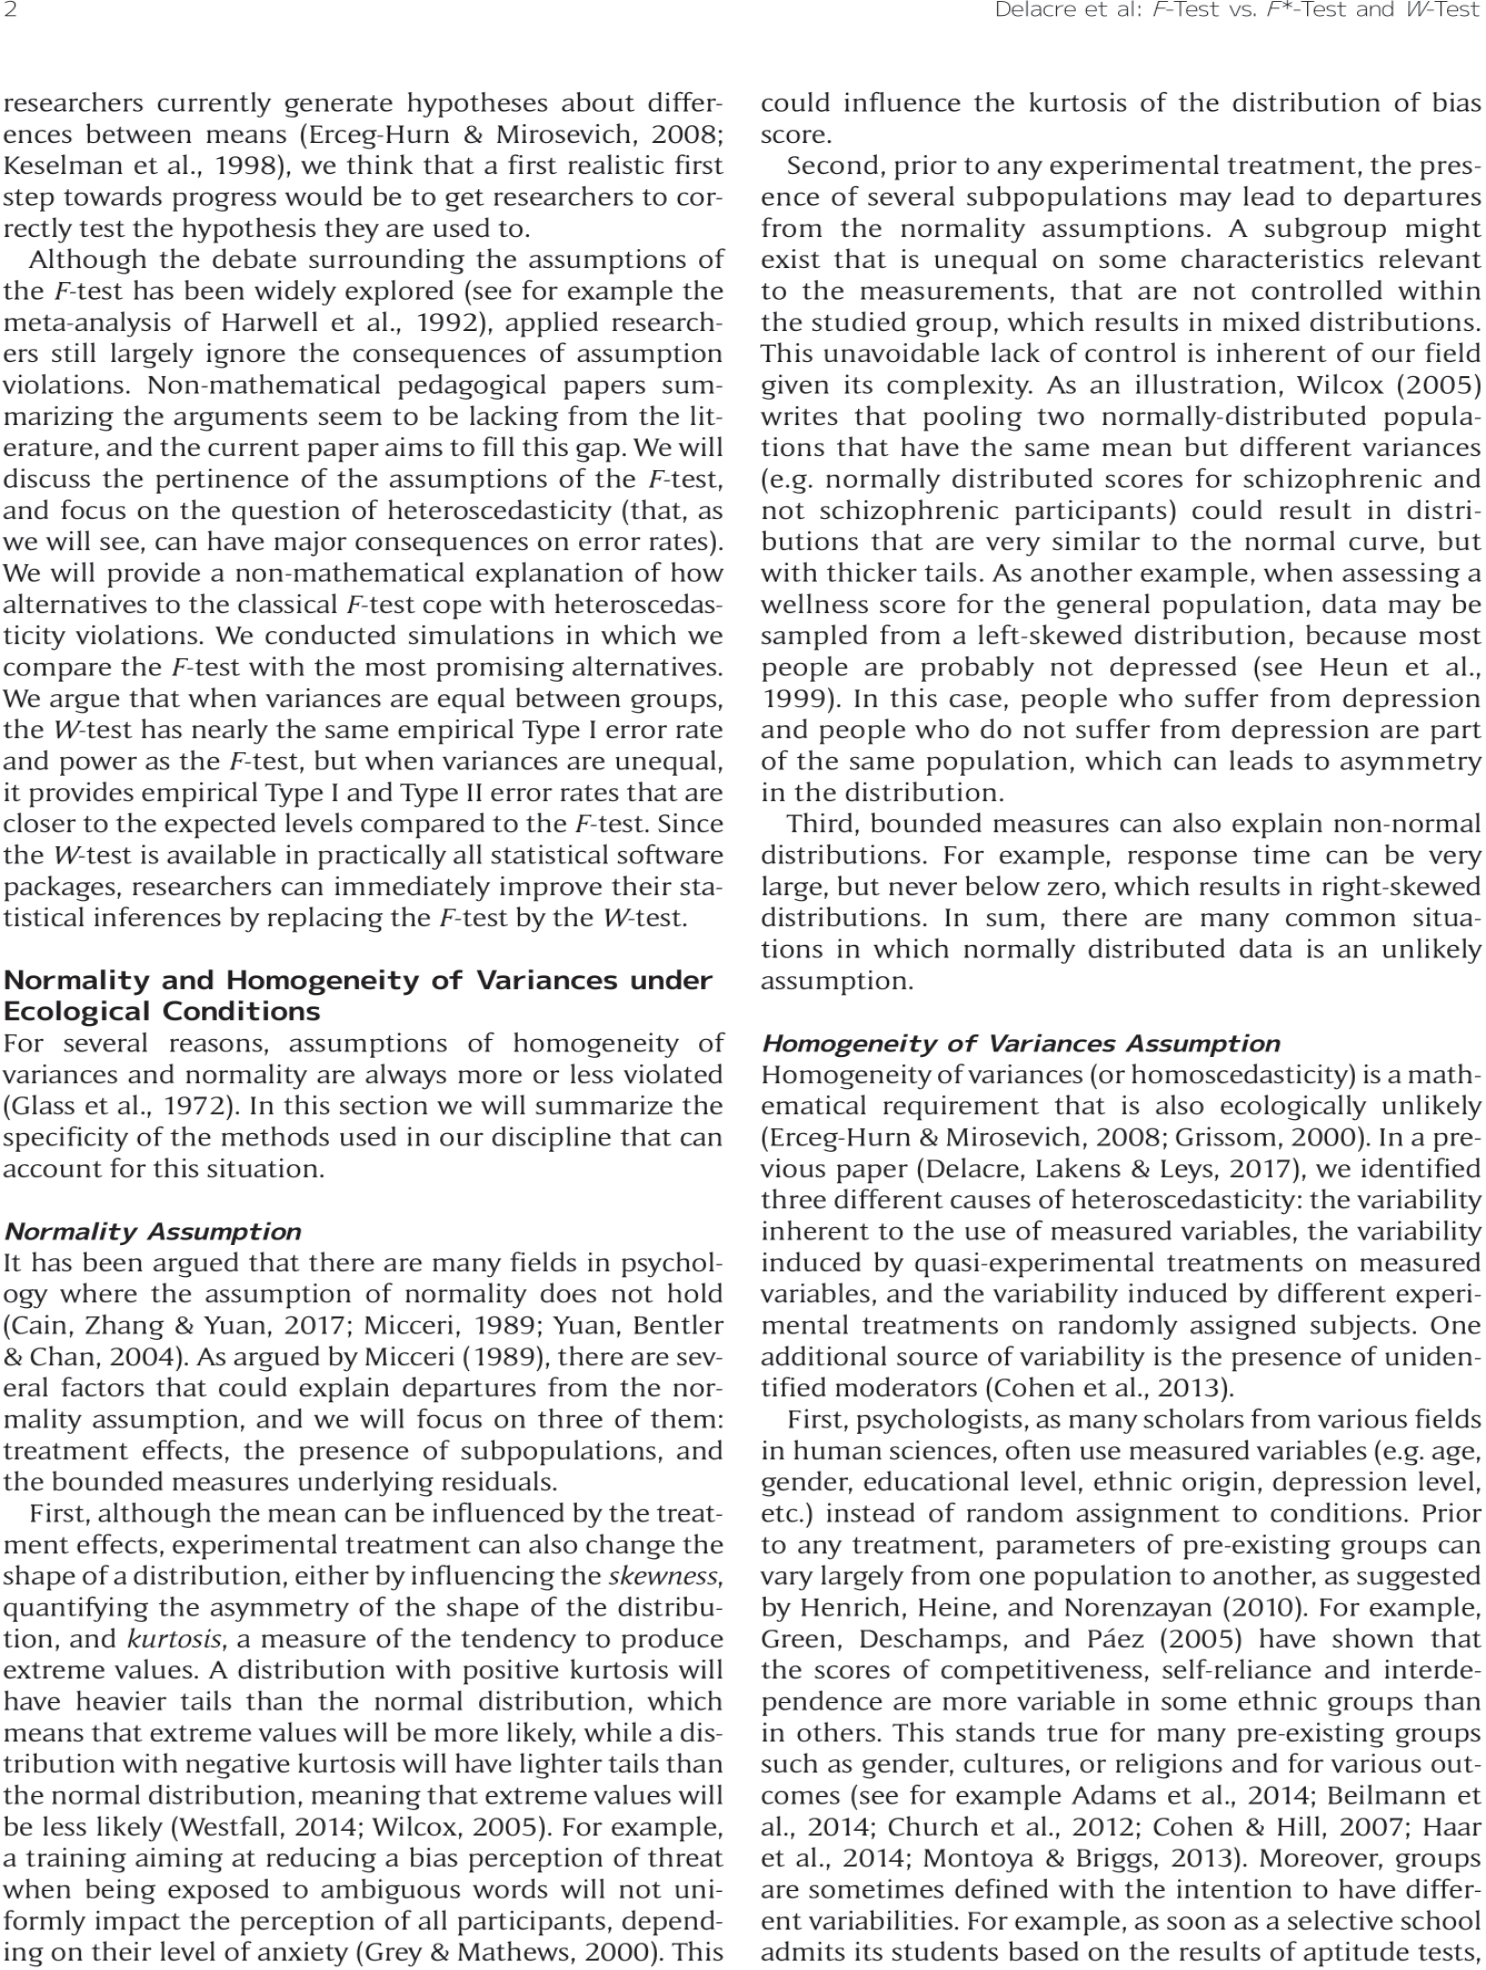
\includegraphics{C:/Users/Admin/Documents/Github projects/thesis/Chapitre 3/Chapitre 3-2} \end{center}

\begin{center}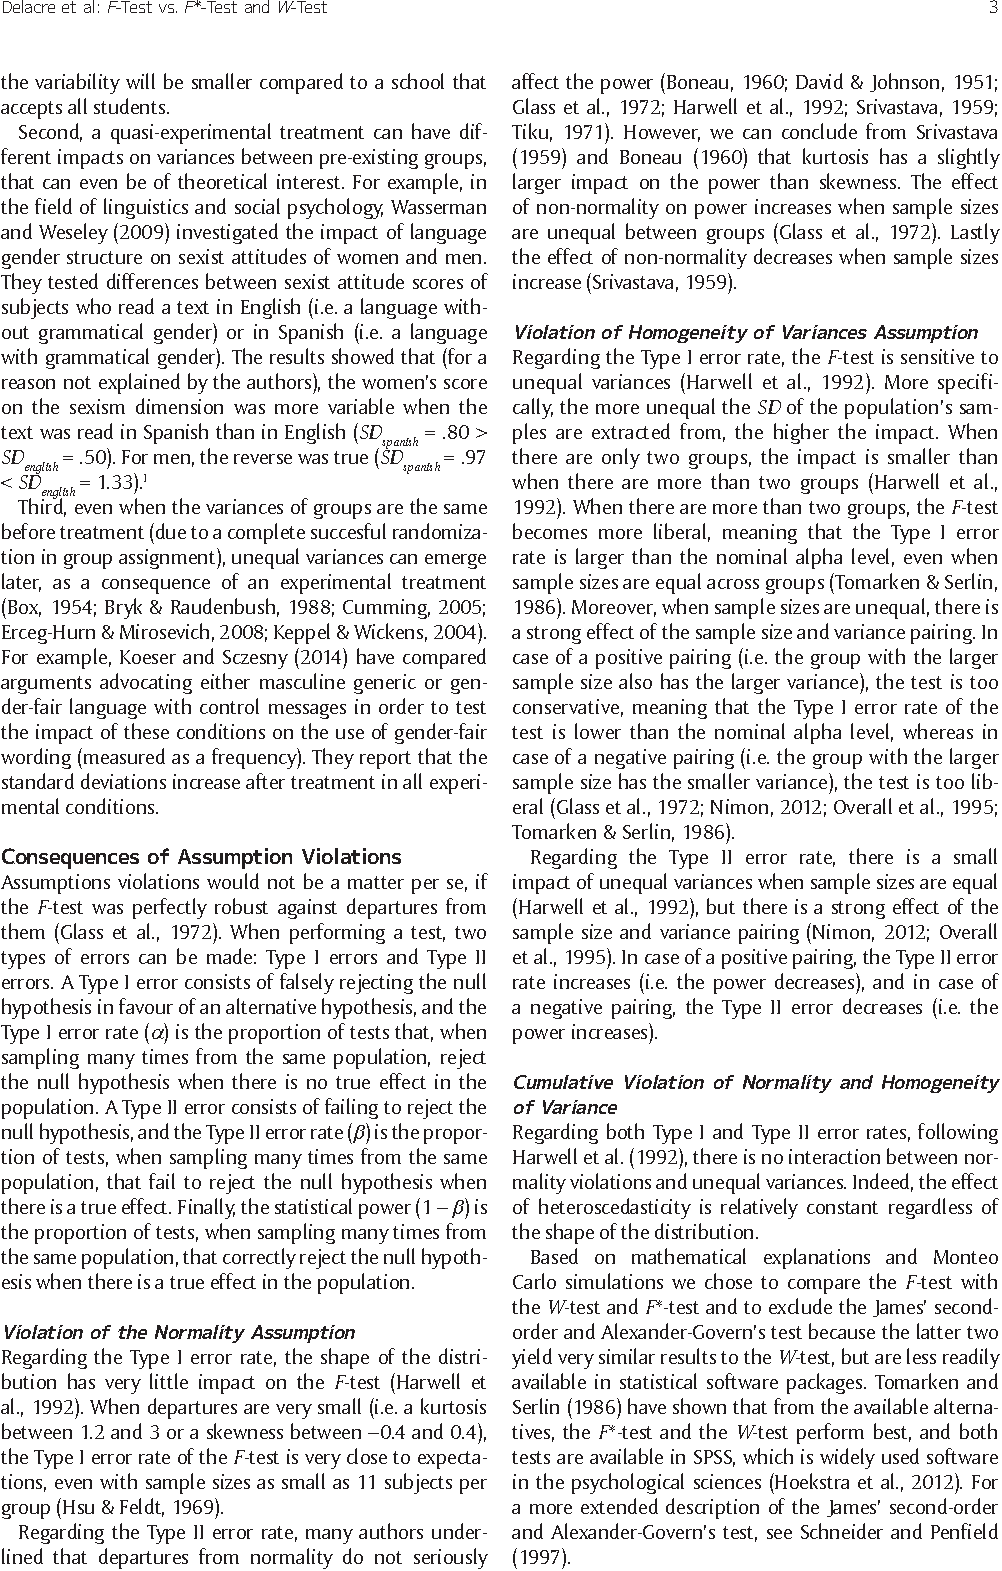
\includegraphics{C:/Users/Admin/Documents/Github projects/thesis/Chapitre 3/Chapitre 3-3} \end{center}

\begin{center}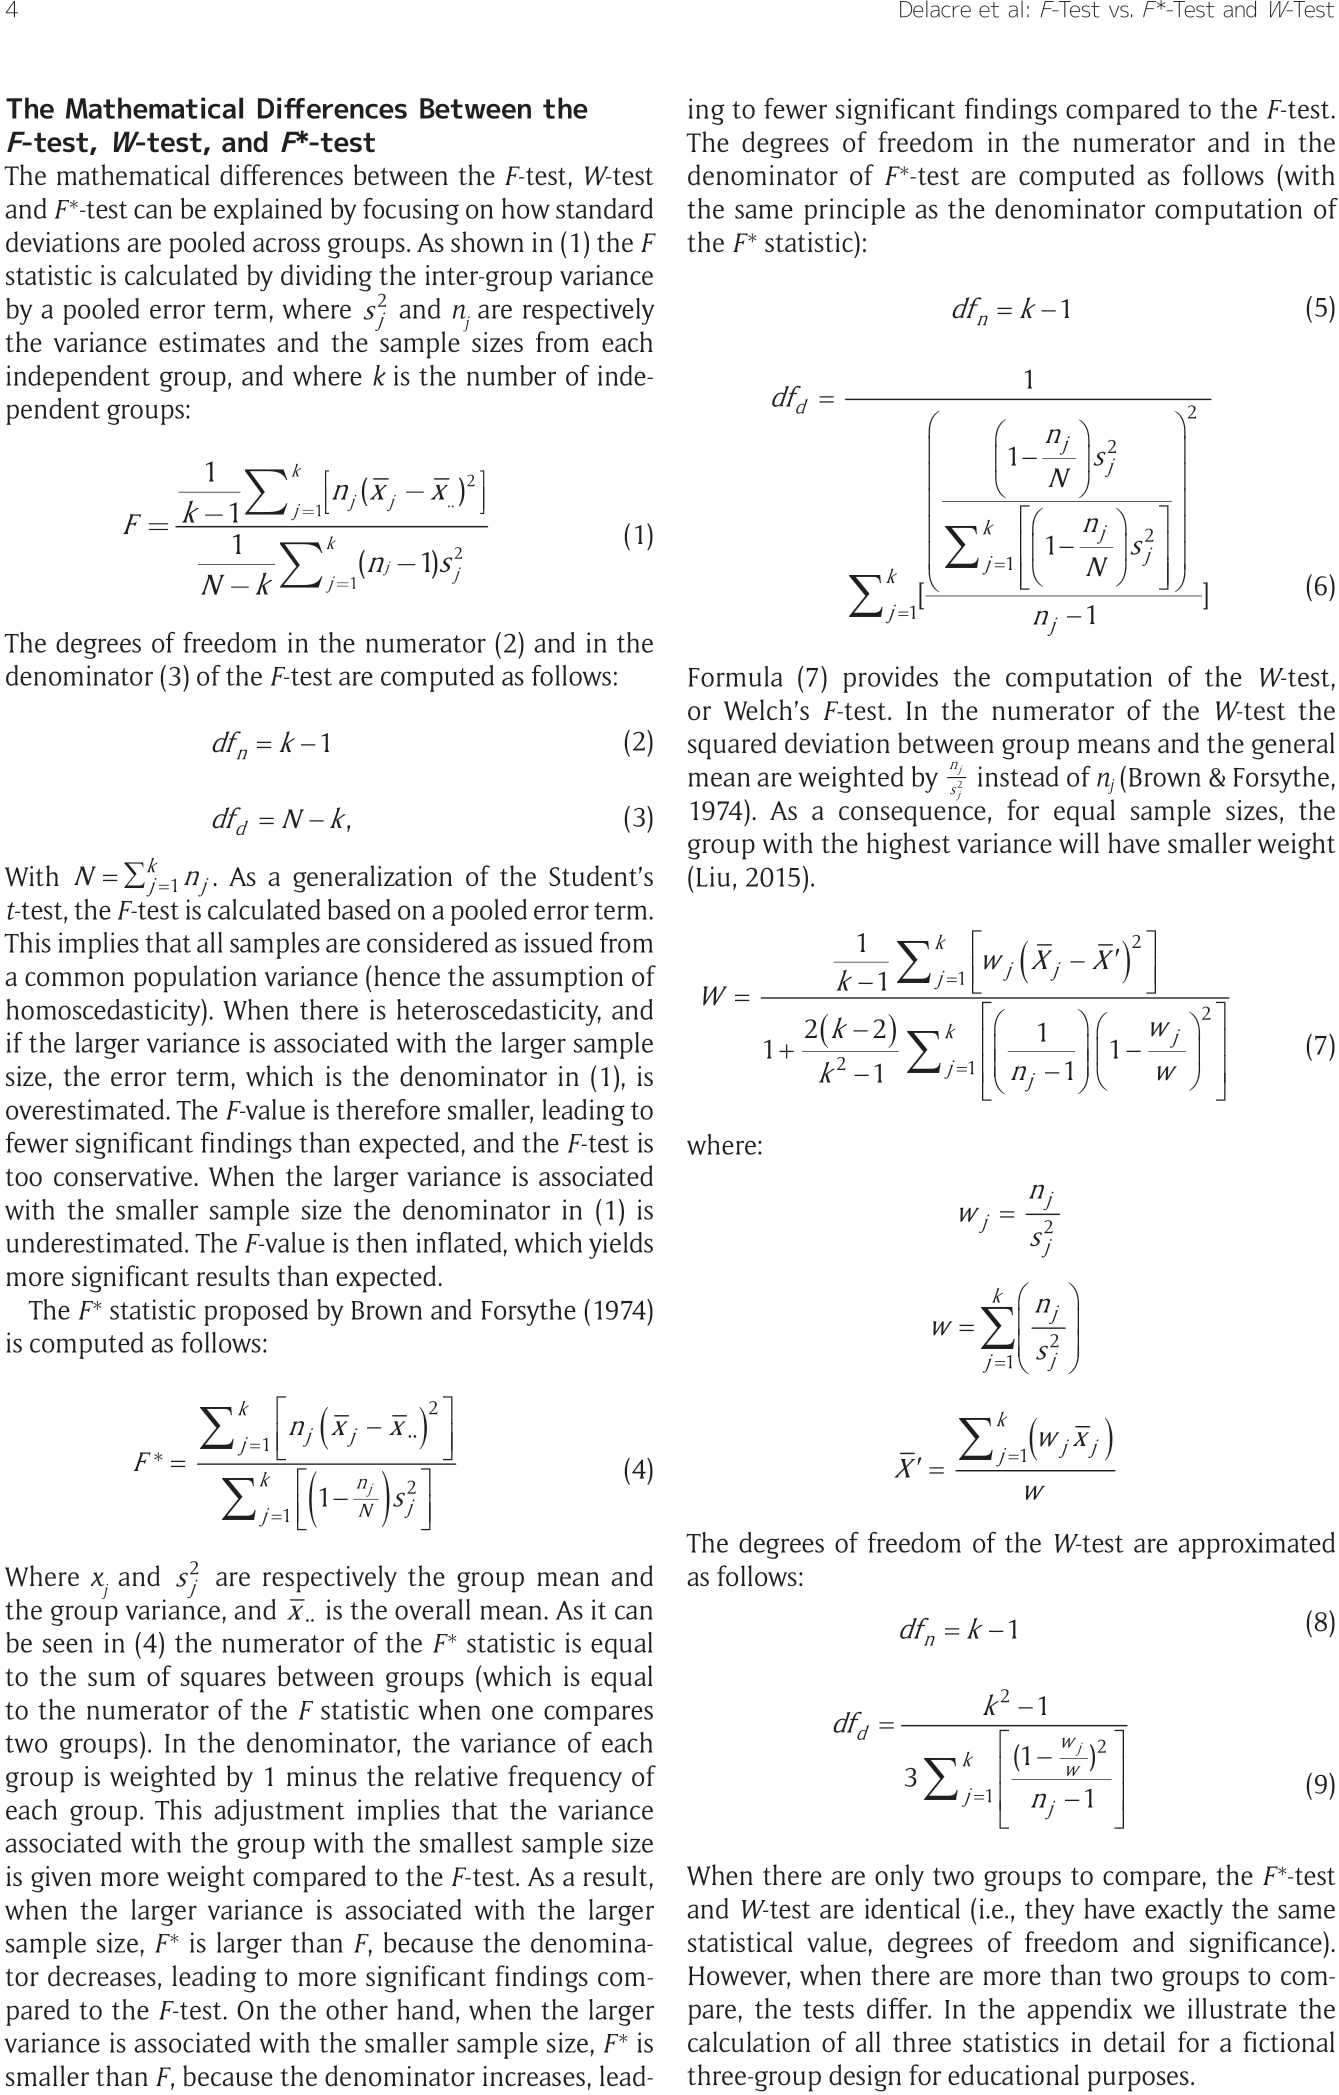
\includegraphics{C:/Users/Admin/Documents/Github projects/thesis/Chapitre 3/Chapitre 3-4} \end{center}

\begin{center}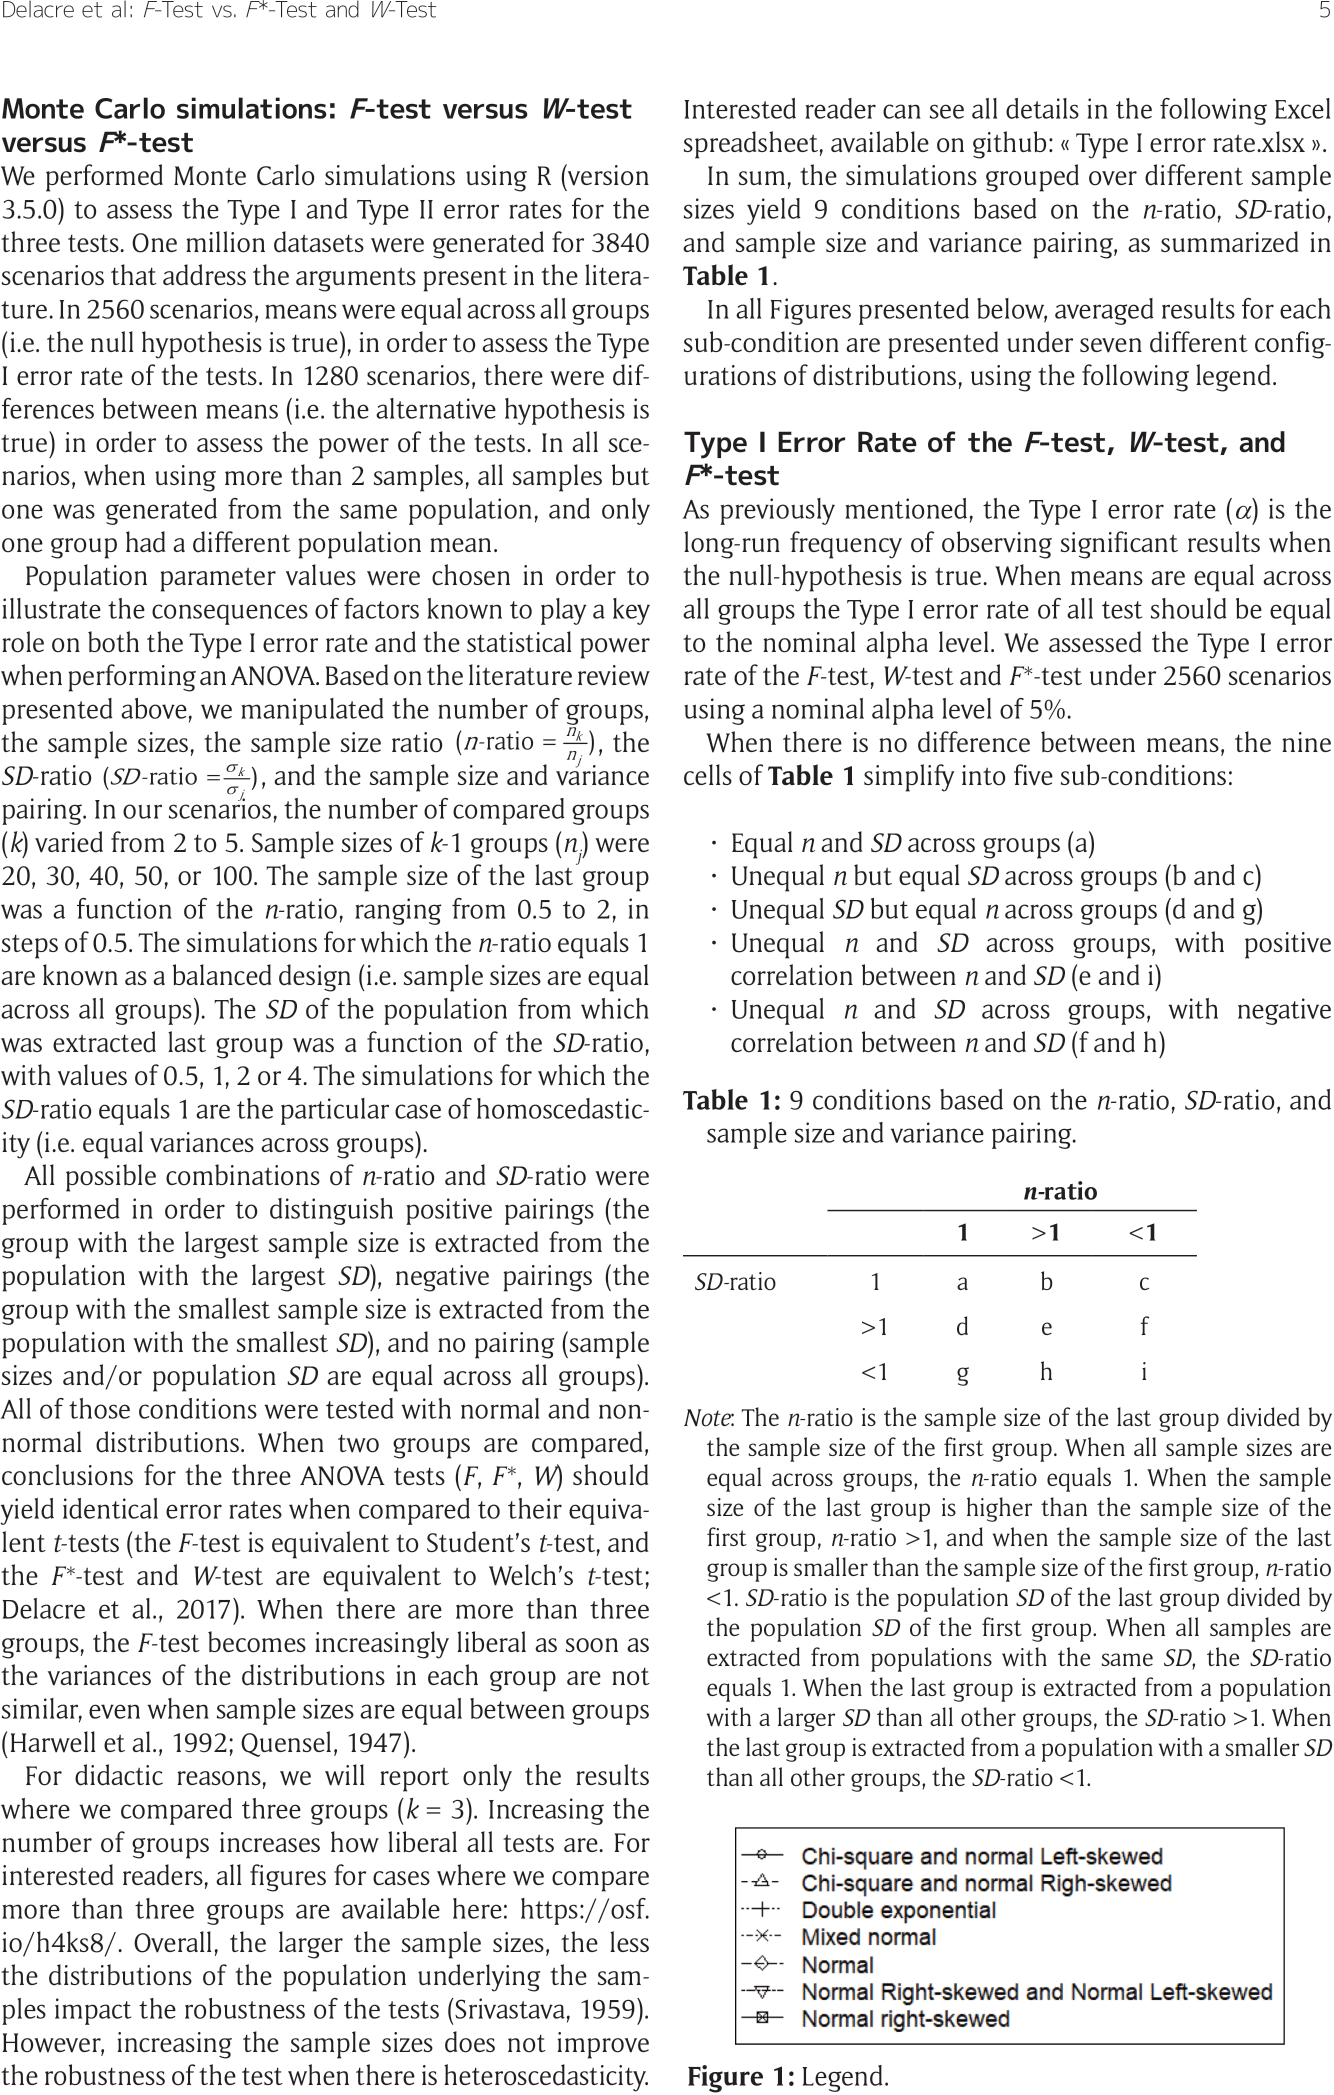
\includegraphics{C:/Users/Admin/Documents/Github projects/thesis/Chapitre 3/Chapitre 3-5} \end{center}

\begin{center}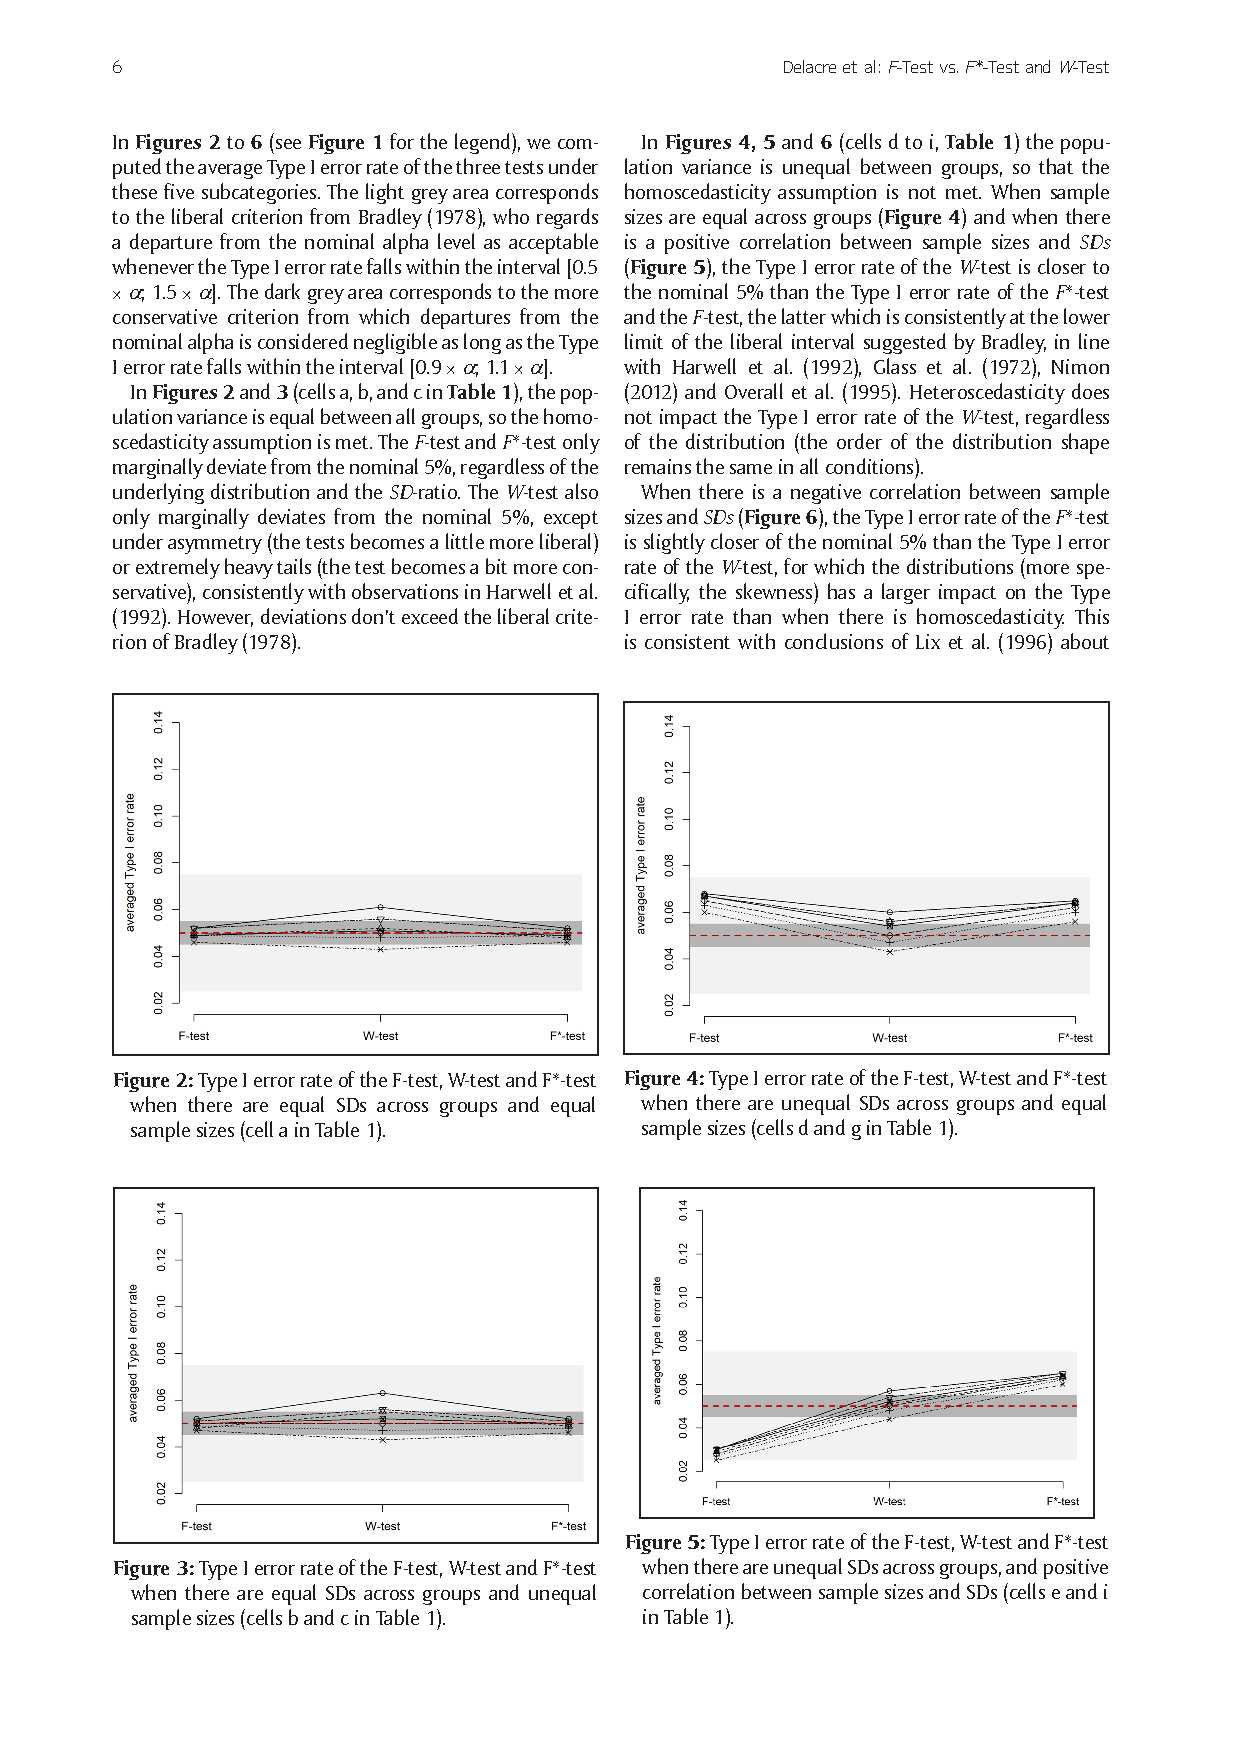
\includegraphics{C:/Users/Admin/Documents/Github projects/thesis/Chapitre 3/Chapitre 3-6} \end{center}

\begin{center}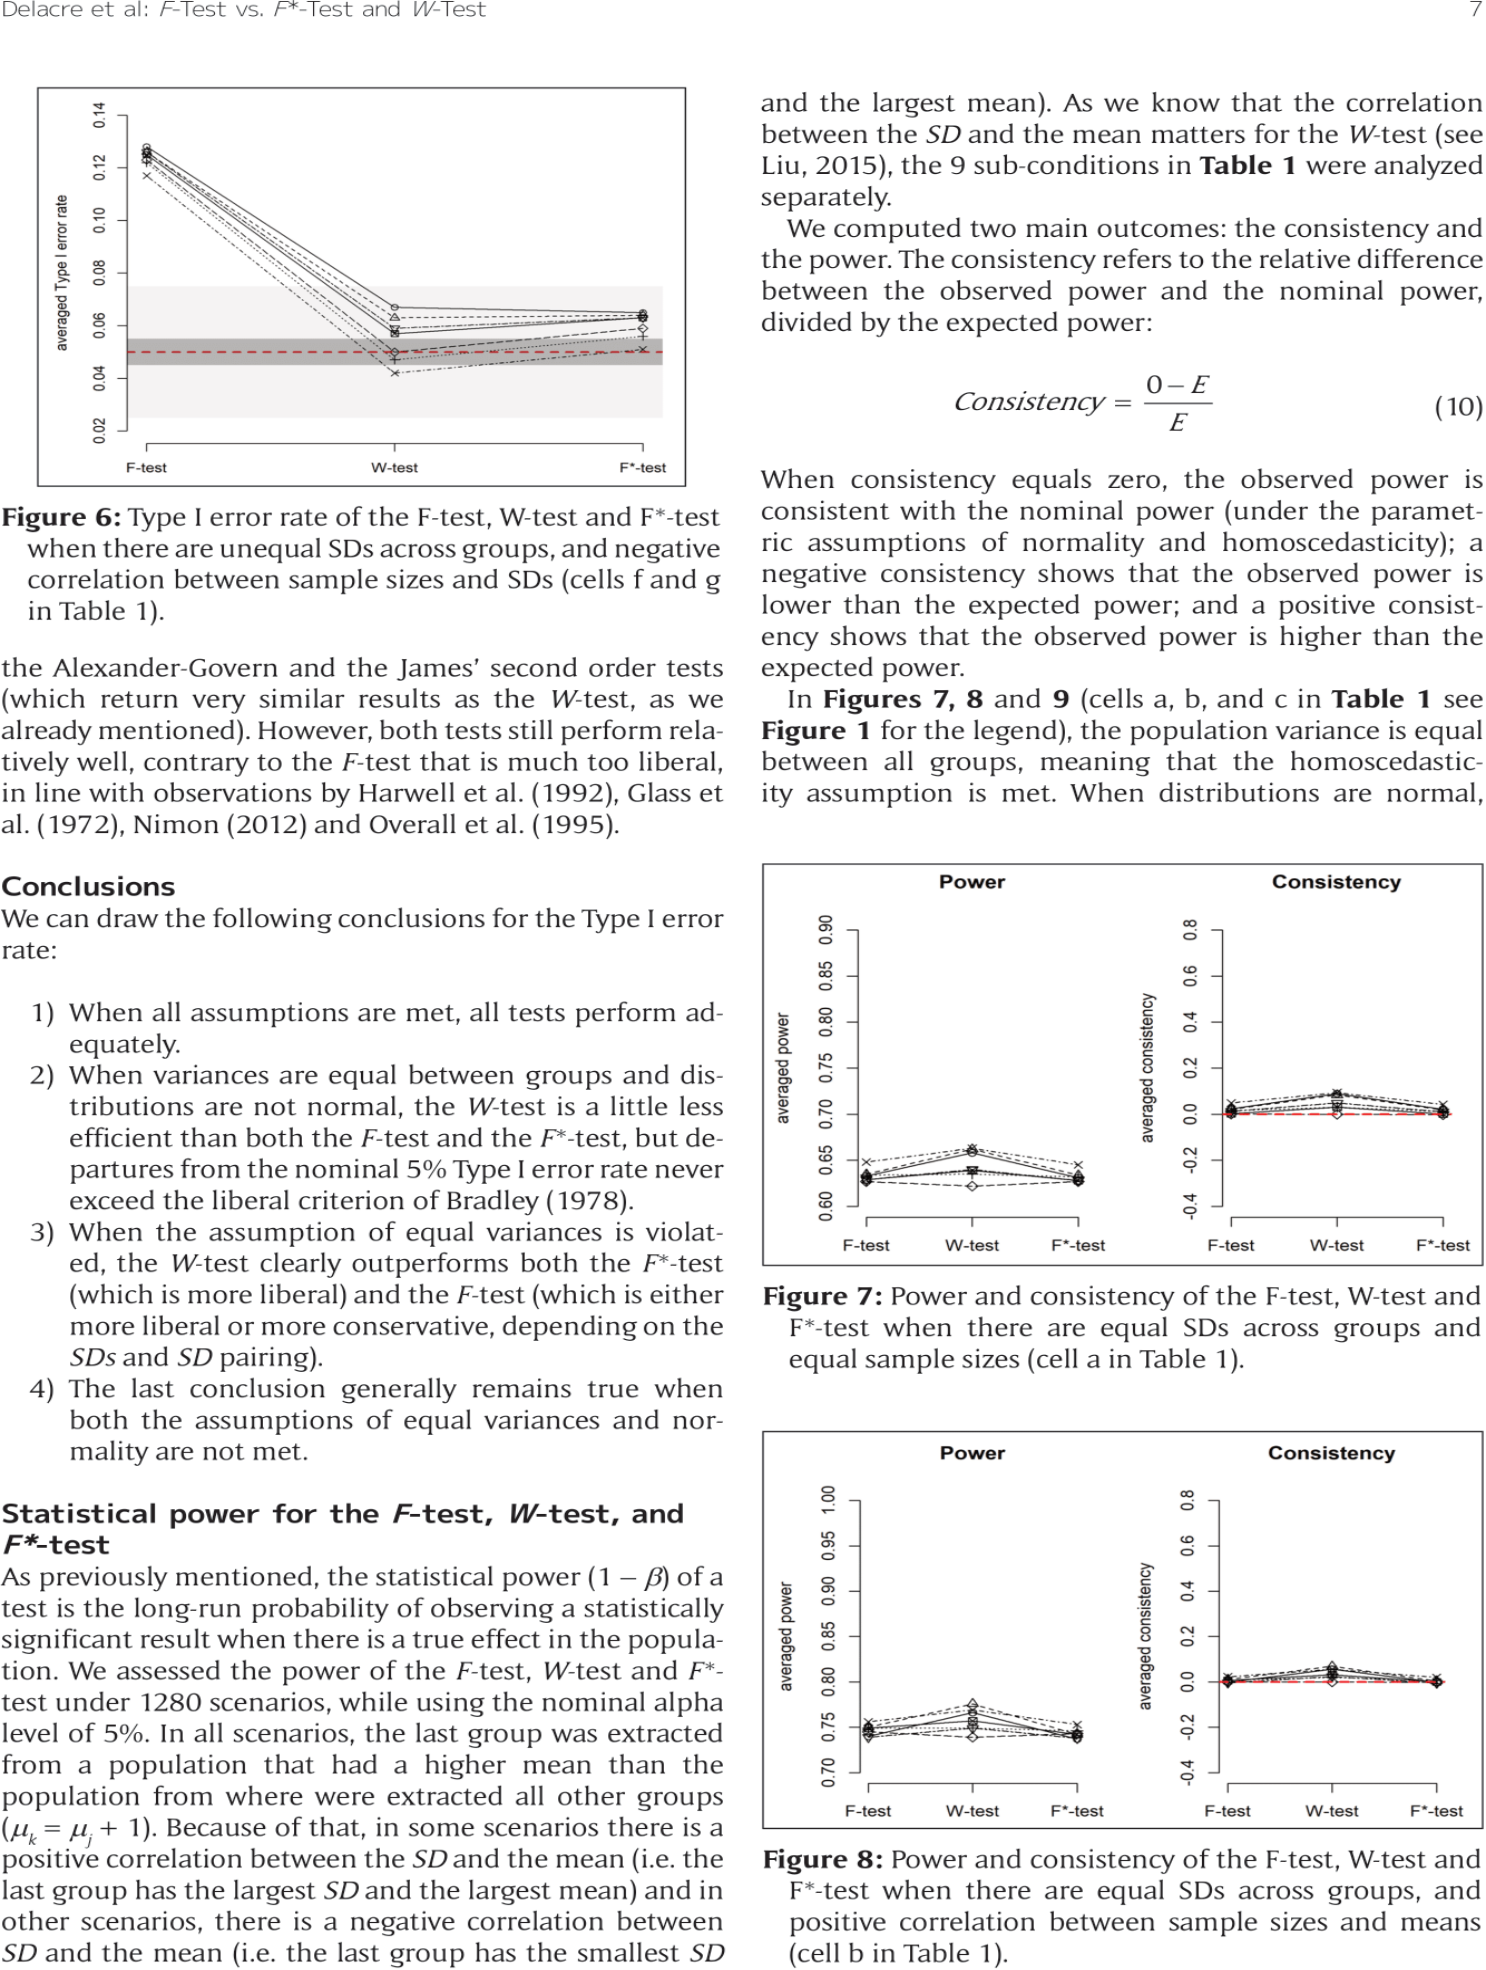
\includegraphics{C:/Users/Admin/Documents/Github projects/thesis/Chapitre 3/Chapitre 3-7} \end{center}

\begin{center}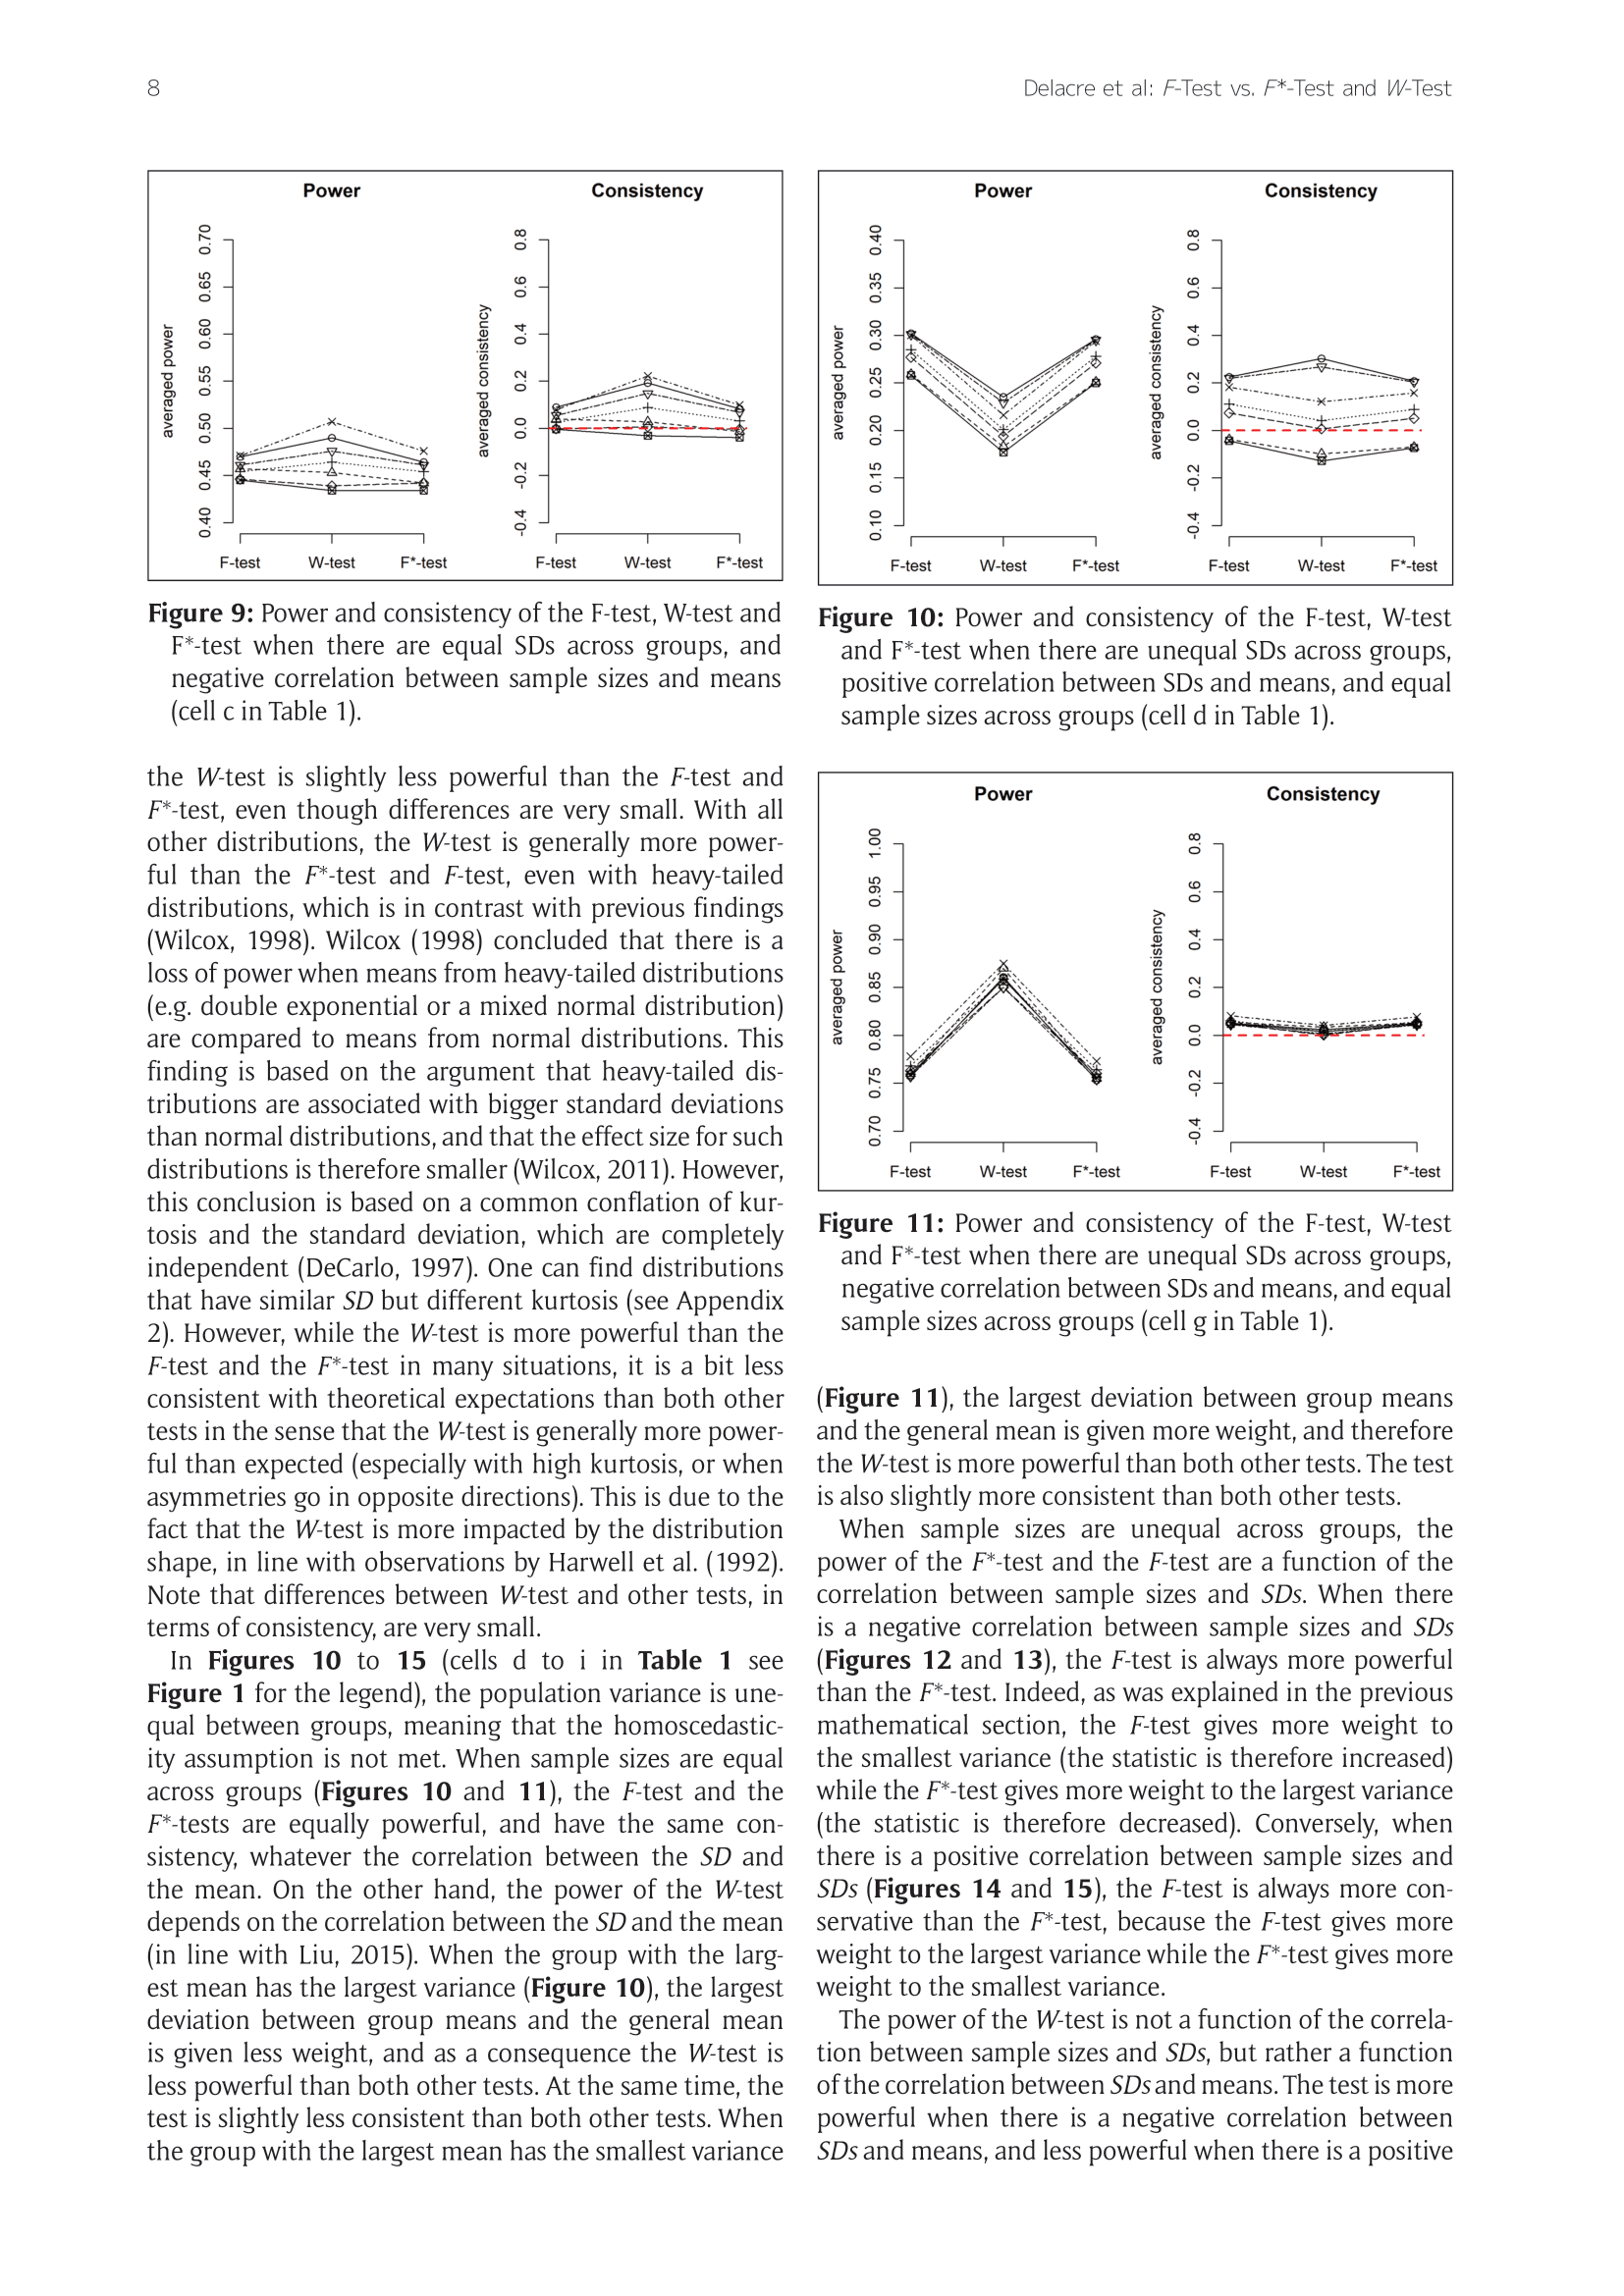
\includegraphics{C:/Users/Admin/Documents/Github projects/thesis/Chapitre 3/Chapitre 3-8} \end{center}

\begin{center}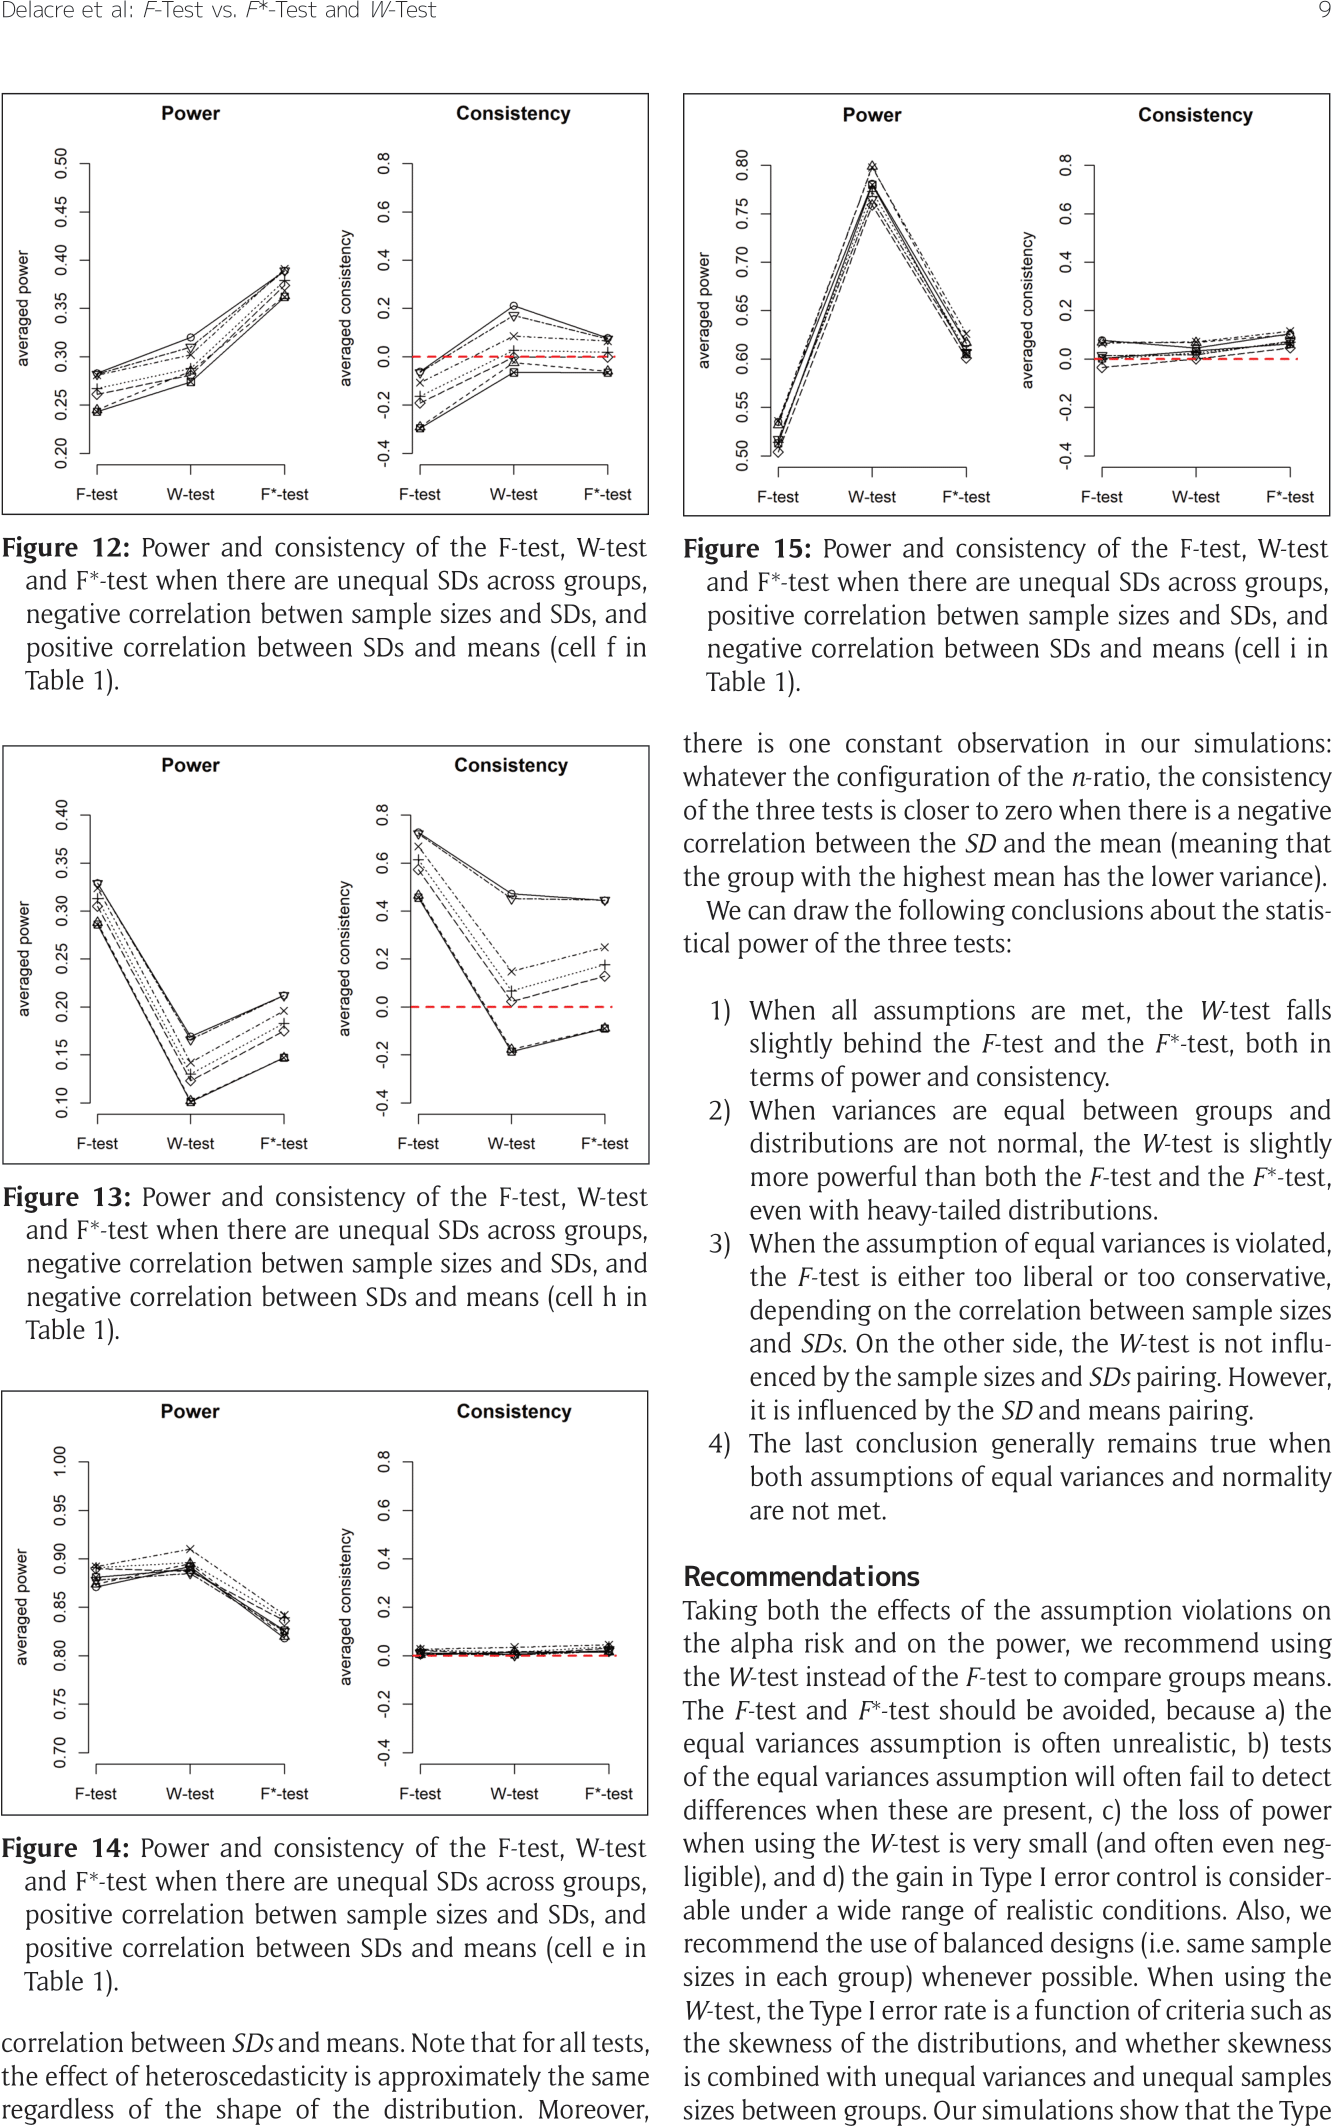
\includegraphics{C:/Users/Admin/Documents/Github projects/thesis/Chapitre 3/Chapitre 3-9} \end{center}

\begin{center}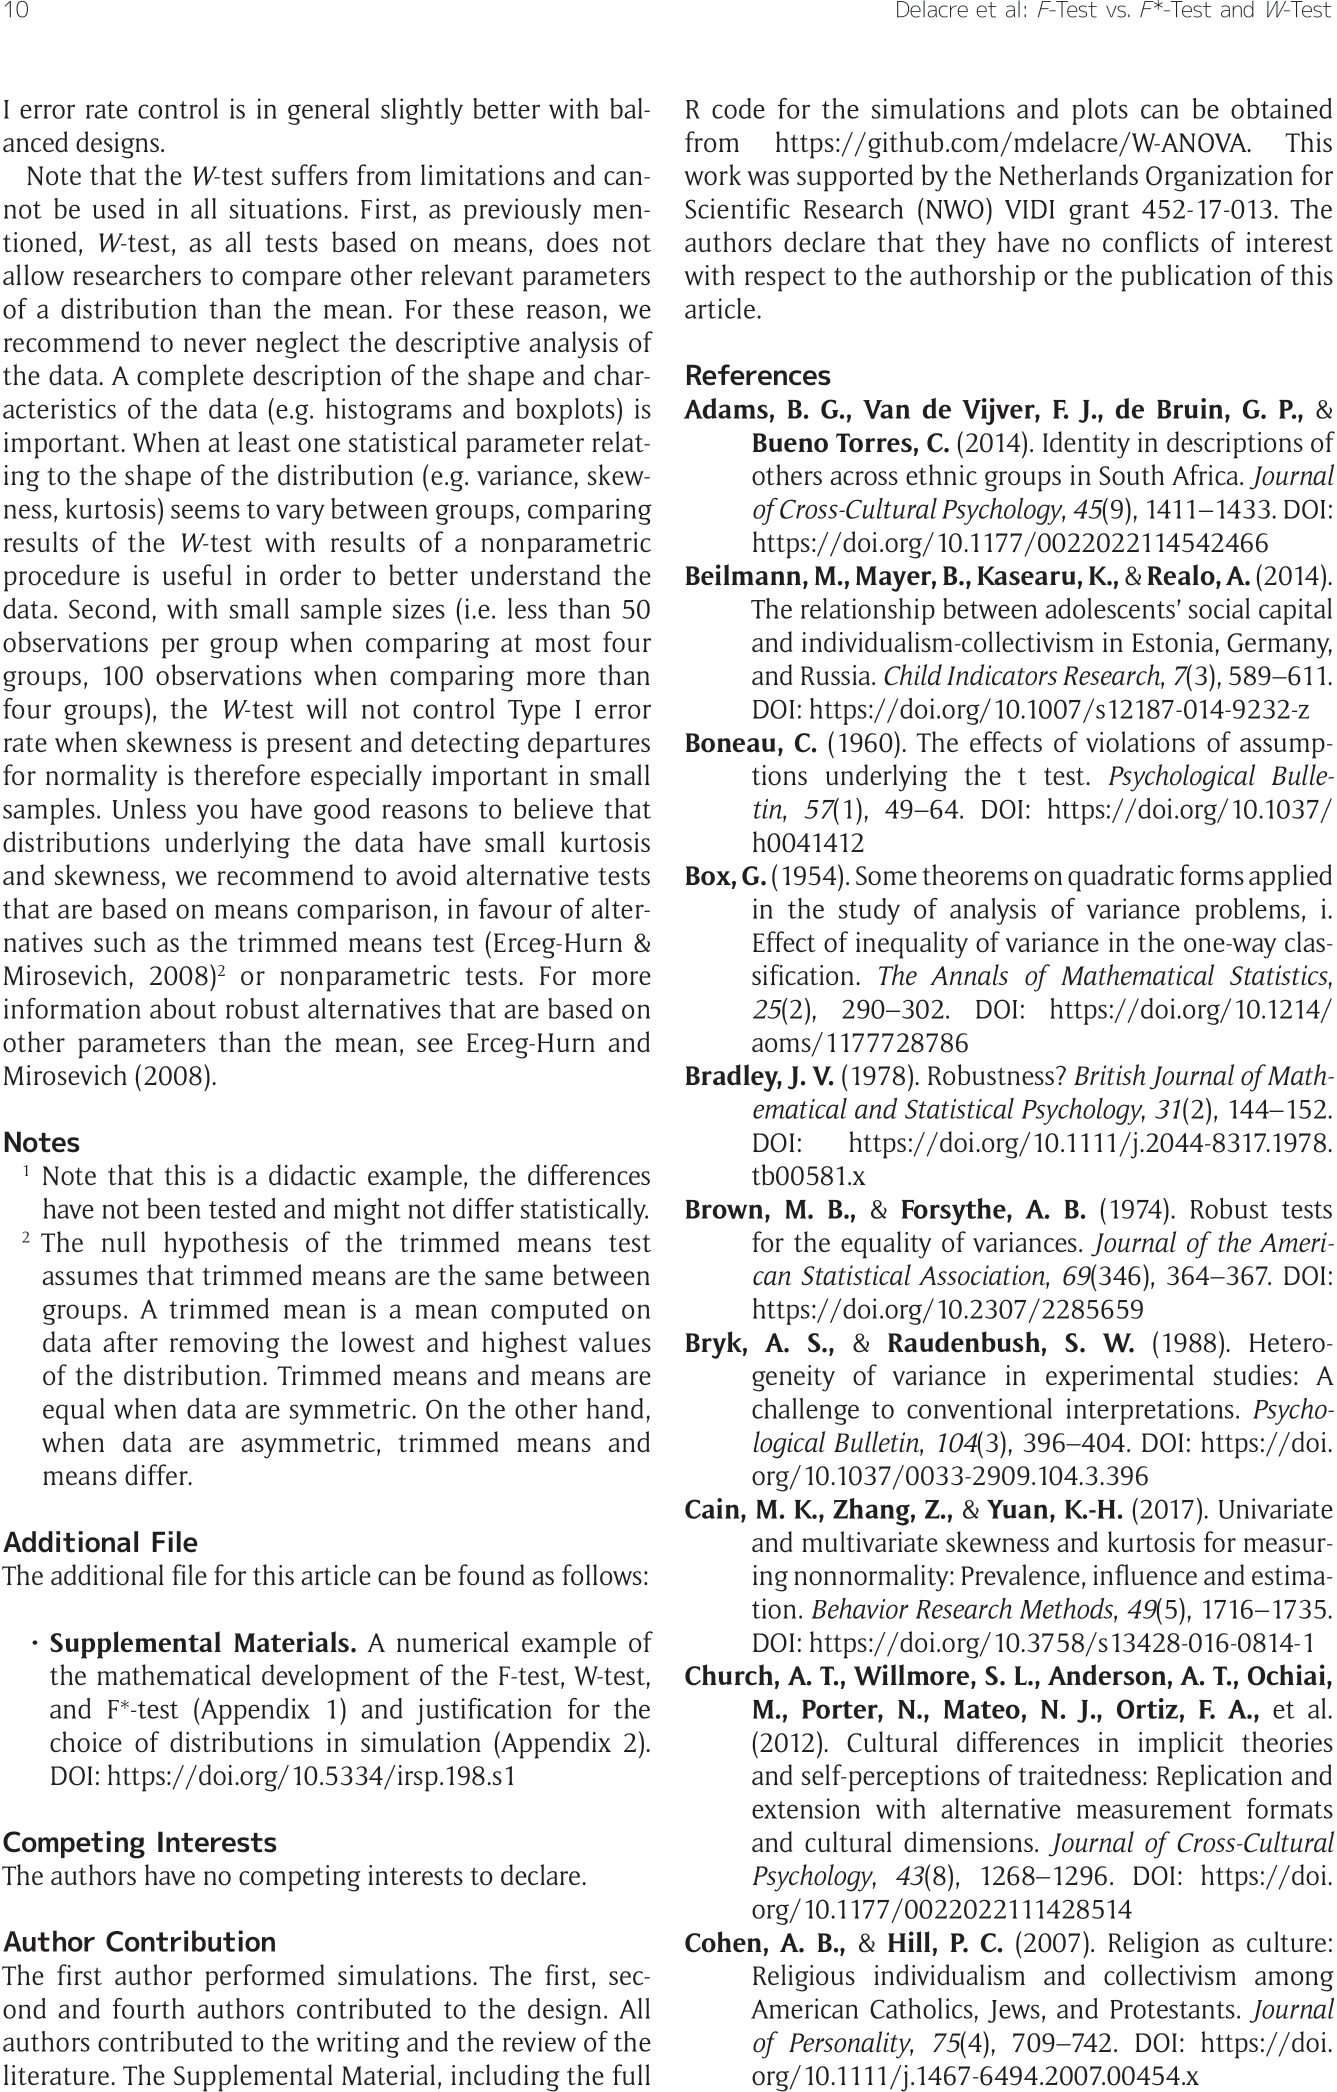
\includegraphics{C:/Users/Admin/Documents/Github projects/thesis/Chapitre 3/Chapitre 3-10} \end{center}

\begin{center}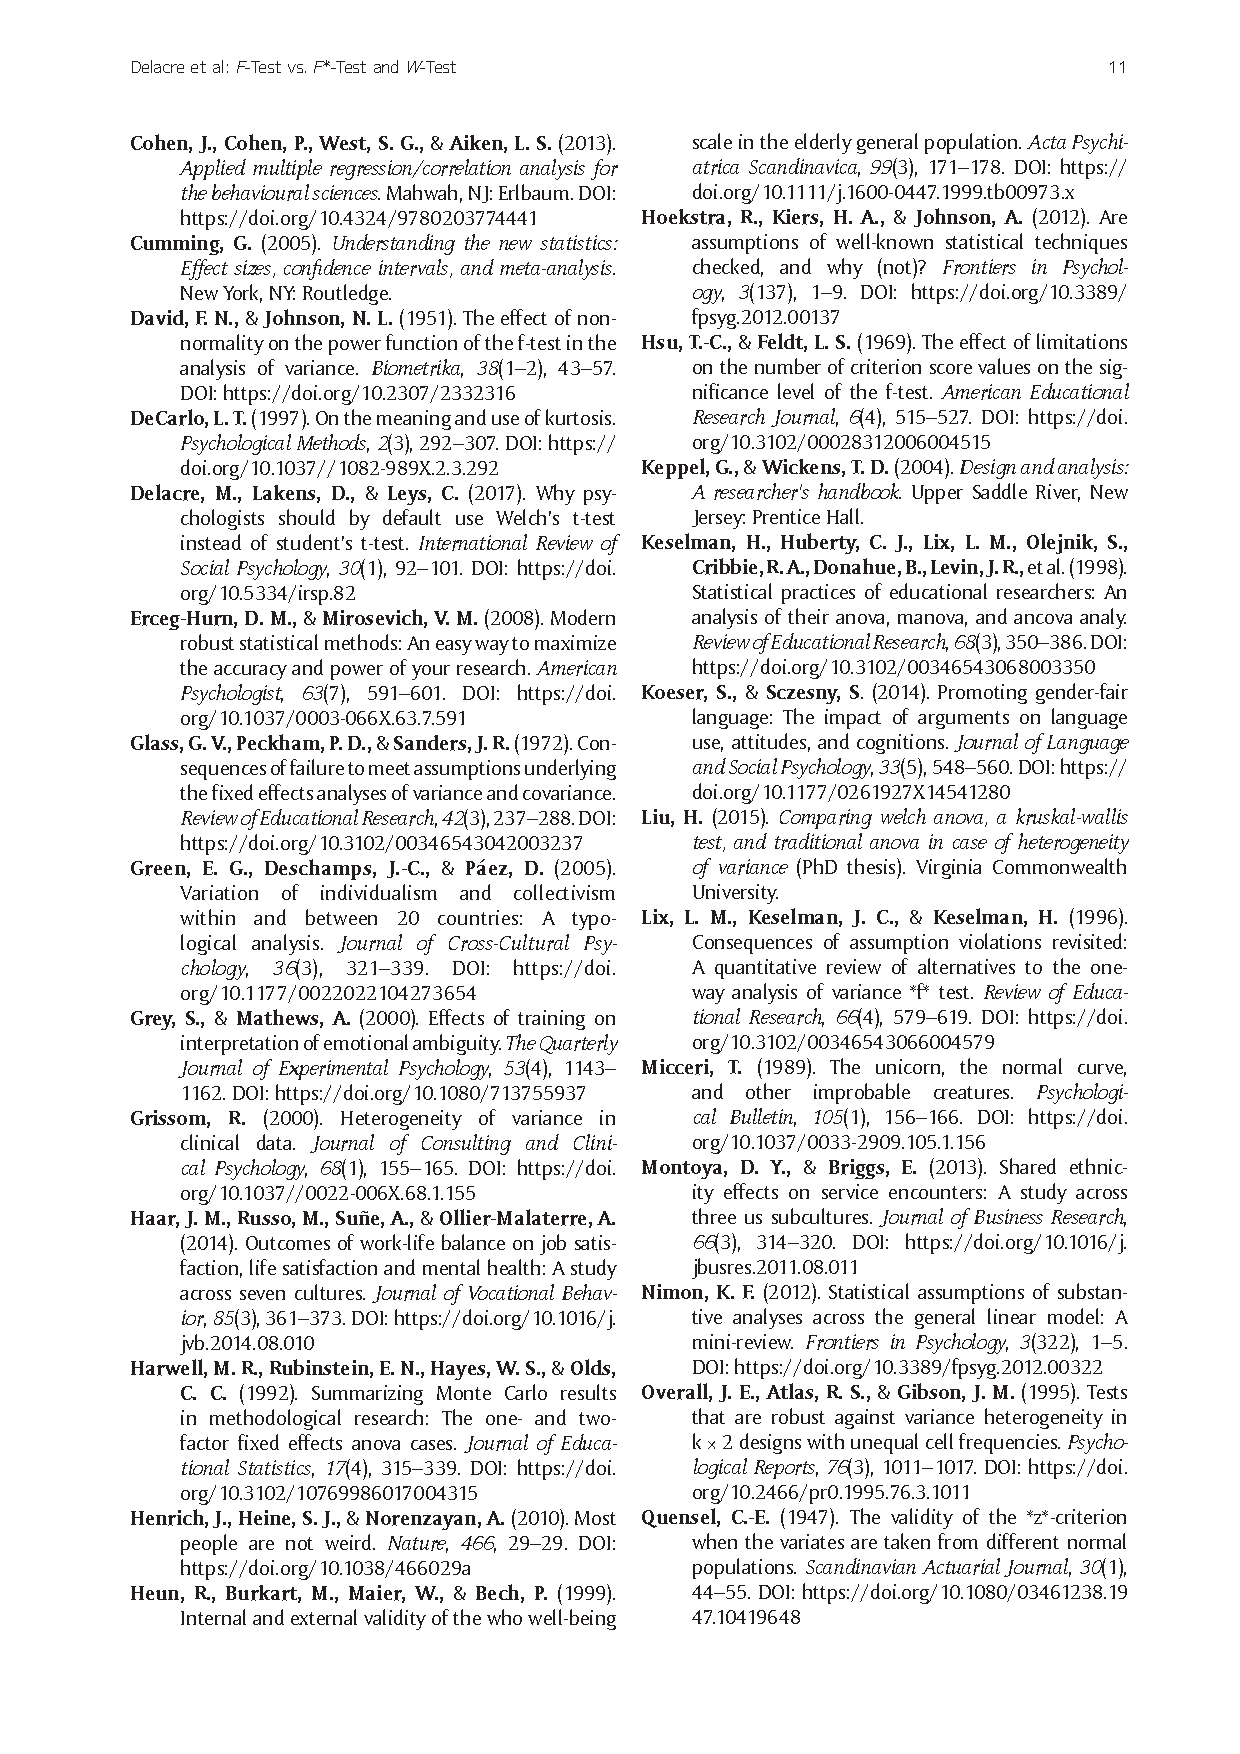
\includegraphics{C:/Users/Admin/Documents/Github projects/thesis/Chapitre 3/Chapitre 3-11} \end{center}

\begin{center}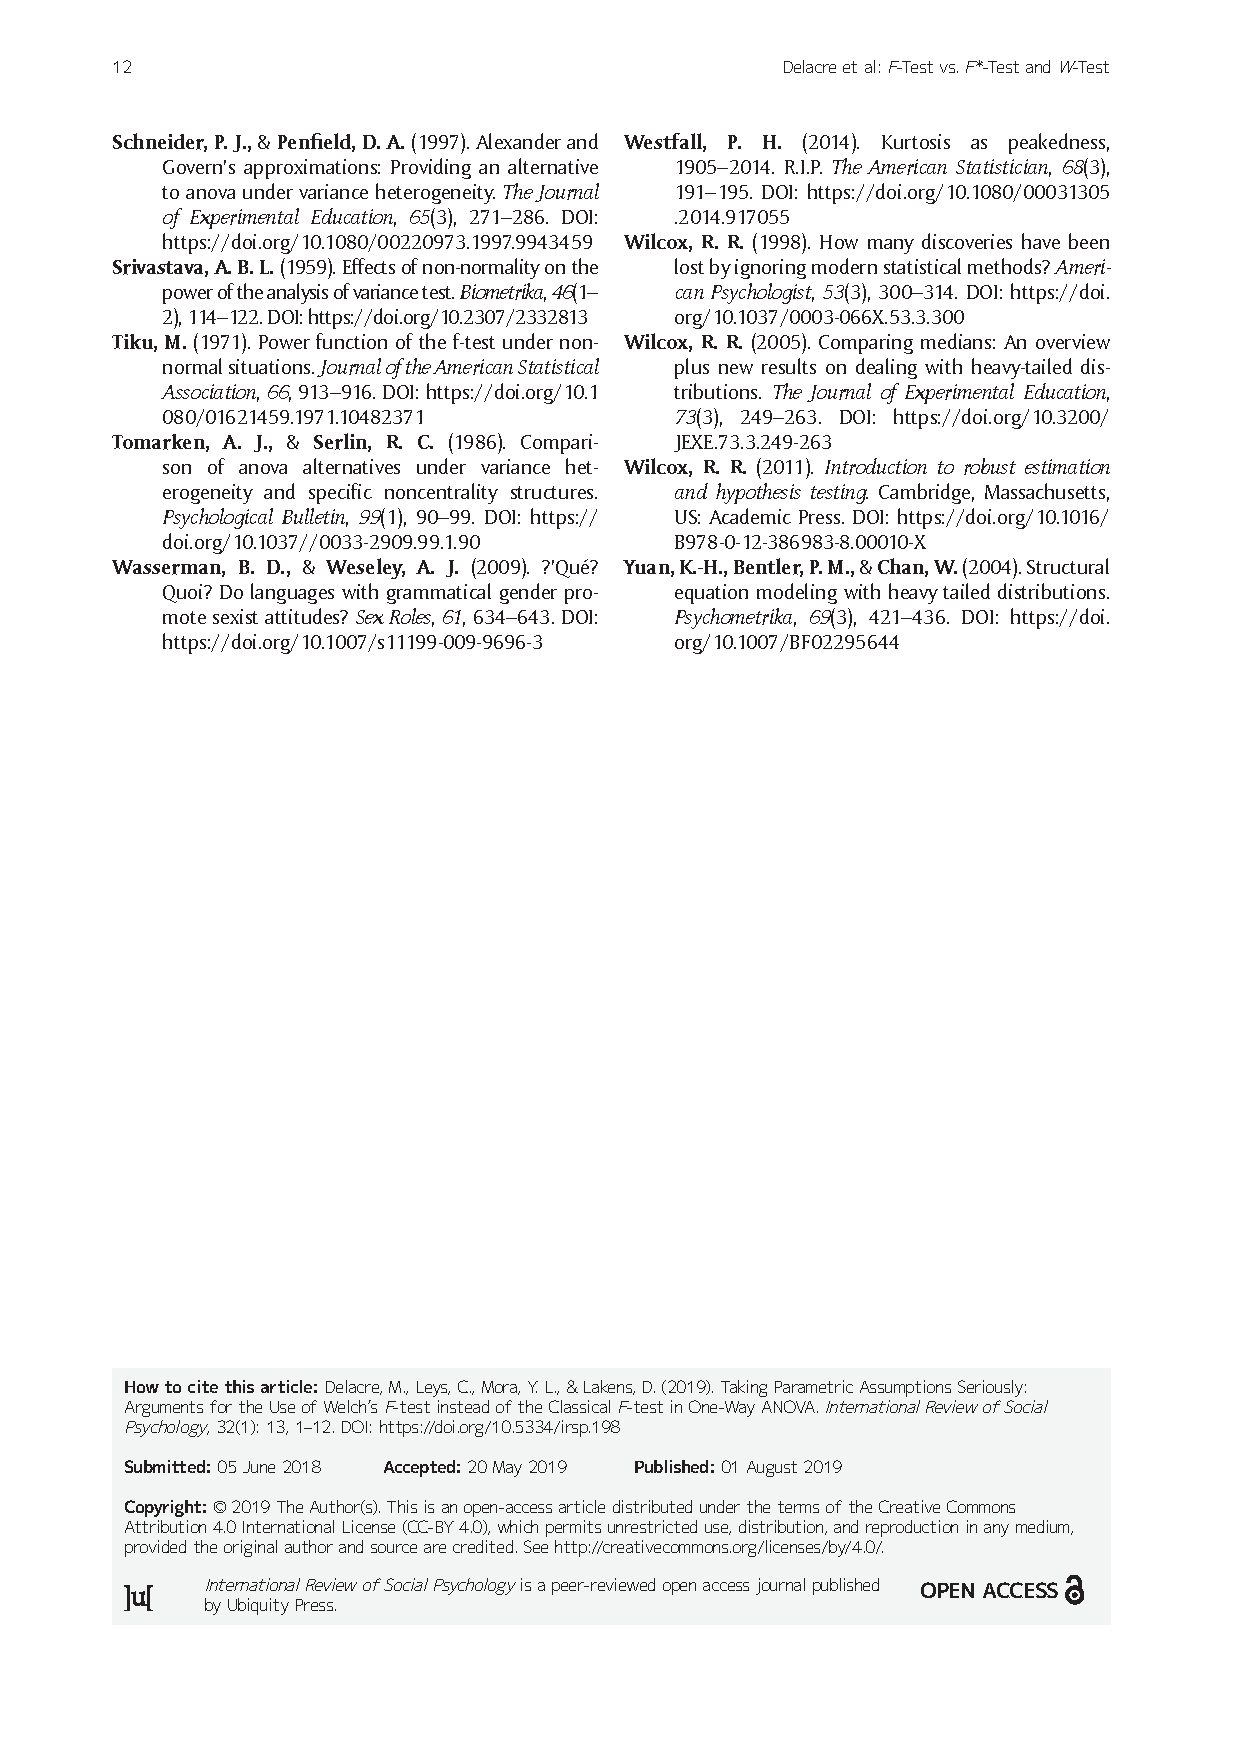
\includegraphics[width=0.82\linewidth]{C:/Users/Admin/Documents/Github projects/thesis/Chapitre 3/Chapitre 3-12} \end{center}

\begingroup
\parindent 0pt
\renewcommand\notesname{{\normalsize Note de fin de chapitre}}

\parskip 1ex \theendnotes \endgroup

\newpage

\hypertarget{chapitre-4-utiliser-le-bmg-de-hedges-basuxe9-sur-luxe9cart-type-non-pooluxe9}{%
\section{\texorpdfstring{Chapitre 4: Utiliser le \(\bm{g^*}\) de Hedges
basé sur l'écart-type non
poolé}{Chapitre 4: Utiliser le \textbackslash bm\{g\^{}*\} de Hedges basé sur l'écart-type non poolé}}\label{chapitre-4-utiliser-le-bmg-de-hedges-basuxe9-sur-luxe9cart-type-non-pooluxe9}}

\begin{center}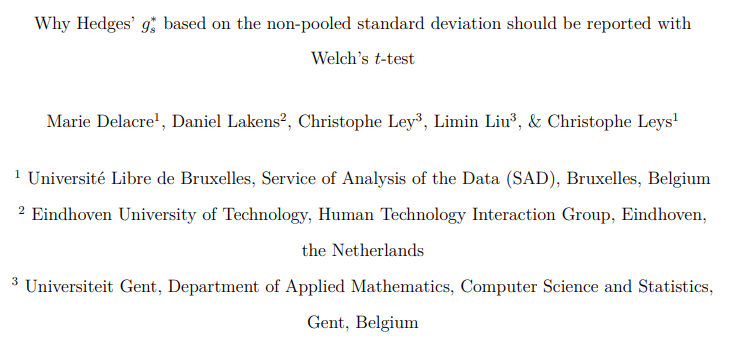
\includegraphics[width=1.5\linewidth]{C:/Users/Admin/Documents/Github projects/thesis/Chapitre 4/title.png
} \end{center}

\begin{center}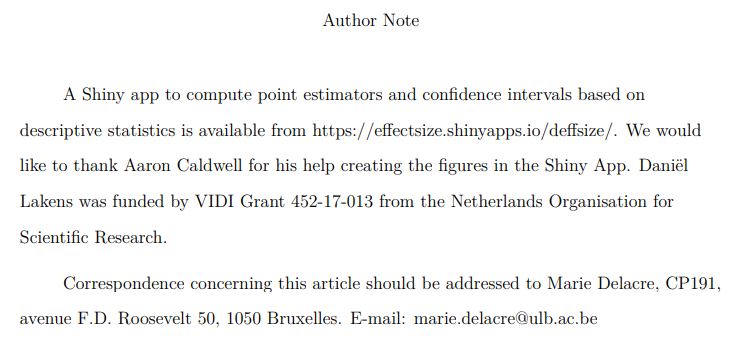
\includegraphics[width=1.5\linewidth]{C:/Users/Admin/Documents/Github projects/thesis/Chapitre 4/authornote.png
} \end{center}

\textbf{Commentaire}: l'article présenté ci-dessous n'a pas encore été
accepté pour publication. Nous tenterons prochainement une nouvelle
soumission, après avoir inclus une série de modifications suggérées par
Geoff Cumming, conformément aux échanges reportés dans l'annexe C (pour
l'instant, la seule modification prise en compte est le conseil de
supprimer tous les indices ``\(_s\)'' associés aux mesure de taille
d'effet).

\newpage

Effect sizes are an important outcome of empirical research. Moving
beyond decisions about statistical significance, there is a strong call
for researchers to report and interpret effect sizes and associated
confidence intervals. This practice is highly endorsed by the American
Psychological Association (APA) and the American Educational Research
Association (Association, 2010~; Duran et al., 2006).

In ``between-subject'' designs where individuals are randomly assigned
into one of two independent groups and group scores are compared based
on their means, the dominant estimator of effect size is Cohen's \(d\),
where the sample mean difference is divided by the pooled sample
standard deviation (Peng, Chen, Chiang, \& Chiang, 2013~; Shieh, 2013).
This estimator is available in many statistical software packages, such
as SPSS and Stata. However, computing the pooled sample standard
deviation assumes that both sample variances are estimates of a common
population variance, which is known as the homogeneity of variance
assumption. It has been widely argued that there are many fields in
psychology where this assumption is ecologically unlikely (Delacre,
Lakens, \& Leys, 2017~; Erceg-Hurn \& Mirosevich, 2008~; Grissom, 2000).
The question how to deal with the assumption of equal variances has been
widely explored in the context of hypothesis testing, and it is becoming
increasingly common to by default report a \emph{t}-test that does not
assume equal variances, such as Welch's \emph{t}-test.

However, the question which effect size to report when equal variances
are not assumed has received less attention. One possible reason is that
researchers have not found consensus on which of the available options
should be used (Shieh, 2013). Even within the very specific context of
an estimate for the standardized sample mean difference there is little
agreement about which estimator is the best choice. In this article, we
will review the main candidates that have been proposed in the
literature in the \emph{d} family of effect sizes, without (Cohen's
\(d\), Glass's \(d\), Shieh's \(d\) and Cohen's \(d^*\)) and with
correction for bias (Hedges' \(g\), Glass's \(g\), Shieh's \(g\) and
Hedges' \(g^*\)). We provide an R package and Shiny app to compute
relevant effect size measures and their confidence intervals.

Before reviewing the most important effect size measures in the
\emph{d}-family, we will first list the different purposes effect size
measures serve, and discuss the relationship between effect sizes,
statistical, and practical significance. Based on a detailed description
of the good properties an effect size measure should possess, we will
evaluate these properties in the Monte Carlo simulations we performed to
compare the different effect size estimators with correction for bias.

\hypertarget{three-purposes-of-effect-size-estimators}{%
\subsection{Three purposes of effect size
estimators}\label{three-purposes-of-effect-size-estimators}}

The effect size is a measure of the magnitude of an effect. In the
context of the comparison of two groups based on their means, when the
null hypothesis is the absence of effect, \emph{d}-family effect size
estimators estimate the magnitude of the differences between parameters
of two populations groups are extracted from (e.g.~the mean, Peng \&
Chen, 2014). Such a measure can be used for three different purposes.

First, effect size measures can be used for \emph{interpretative}
purposes. They allow researchers to assess the practical significance of
a result (i.e.~statements about the relevance of an effect in real
life). In order to assess the meaningfulness of an effect, we should be
able to relate this effect size estimate with behaviors/meaningful
consequences in the real world (Andersen, McCullagh, \& Wilson, 2007).
This typically involves an analysis of the costs (determined by a
specific context) and the benefits (in part determined by the size of
the effect). It is important to remember an effect size is just a
mathematical indicator of the magnitude of a difference, which depends
on the way a variable is converted into numerical indicator. An effect
size in itself is not a measure of the importance or the relevance of an
effect for real life (even if benchmarks for small, medium, or large
effect sizes might have contributed to such a misinterpretation, Stout
\& Ruble, 1995).

Second, effect size measures can be used for \emph{comparative}
purposes. They allow researchers to assess the stability of results
across designs, analyses, and sample sizes. This includes statistically
comparing and combining the results from two or more studies in a
meta-analysis.

Third, effect size measures can be used for \emph{inferential} purposes.
Hypothesis tests and confidence intervals based on the same statistical
quantity are directly related: if the area of the null hypothesis is out
of the \((1-\alpha)\)-confidence interval, then the hypothesis test
would also result in a \emph{p}-value below the nominal alpha level. At
the same time, the interval provides extra information about the
precision of the sample estimate for inferential purposes (Altman,
2005~; Ellis, 2010), and which effect sizes are excluded. The narrower
the interval, the higher the precision, and the wider the confidence
interval, the more the data lack precision. Effect size measures are
also indirectly related to the hypothesis tests as effect sizes from
previous studies can be used in an a-priori power analysis when planning
a new study (Lakens, 2013~; Prentice \& Miller, 1992~; Stout \& Ruble,
1995~; Sullivan \& Feinn, 2012~; Wilkinson, 1999).

\hypertarget{properties-of-a-good-effect-size-estimator}{%
\subsection{Properties of a good effect size
estimator}\label{properties-of-a-good-effect-size-estimator}}

The empirical value of an estimator (called the \emph{estimate}) depends
on the sample value. Different samples extracted from the same
population will lead to different sample estimates of the population
value. The \emph{sampling distribution} of the estimator is the
distribution of all estimates, based on all possible samples of size
\emph{n} extracted from one population. Studying the sampling
distribution is useful, as it allows us to assess the qualities of an
estimator. More specifically, three desirable properties a good
estimator should possess for inferential purposes are:
\emph{unbiasedness}, \emph{consistency} and \emph{efficiency} (Wackerly,
Mendenhall, \& Scheaffer, 2008).

An estimator is unbiased if the distribution of estimates is centered
around the true population parameter. On the other hand, an estimator is
positively (or negatively) biased if the distribution is centered around
a value that is higher (or lower) than the true population parameter
(see Figure \ref{fig:BIAS}). In other words, examining the bias of an
estimator tells us if estimates are on average accurate. The \emph{bias}
of a point estimator \(\hat{\delta}\) can be computed as
\begin{equation} 
\delta_{bias}=E(\hat{\delta})-\delta
\label{eqn:BIAS}
\end{equation} where \(E(\hat{\delta})\) is the expectation of the
sampling distribution of the estimator and \(\delta\) is the true
(population) parameter.

\begin{figure}
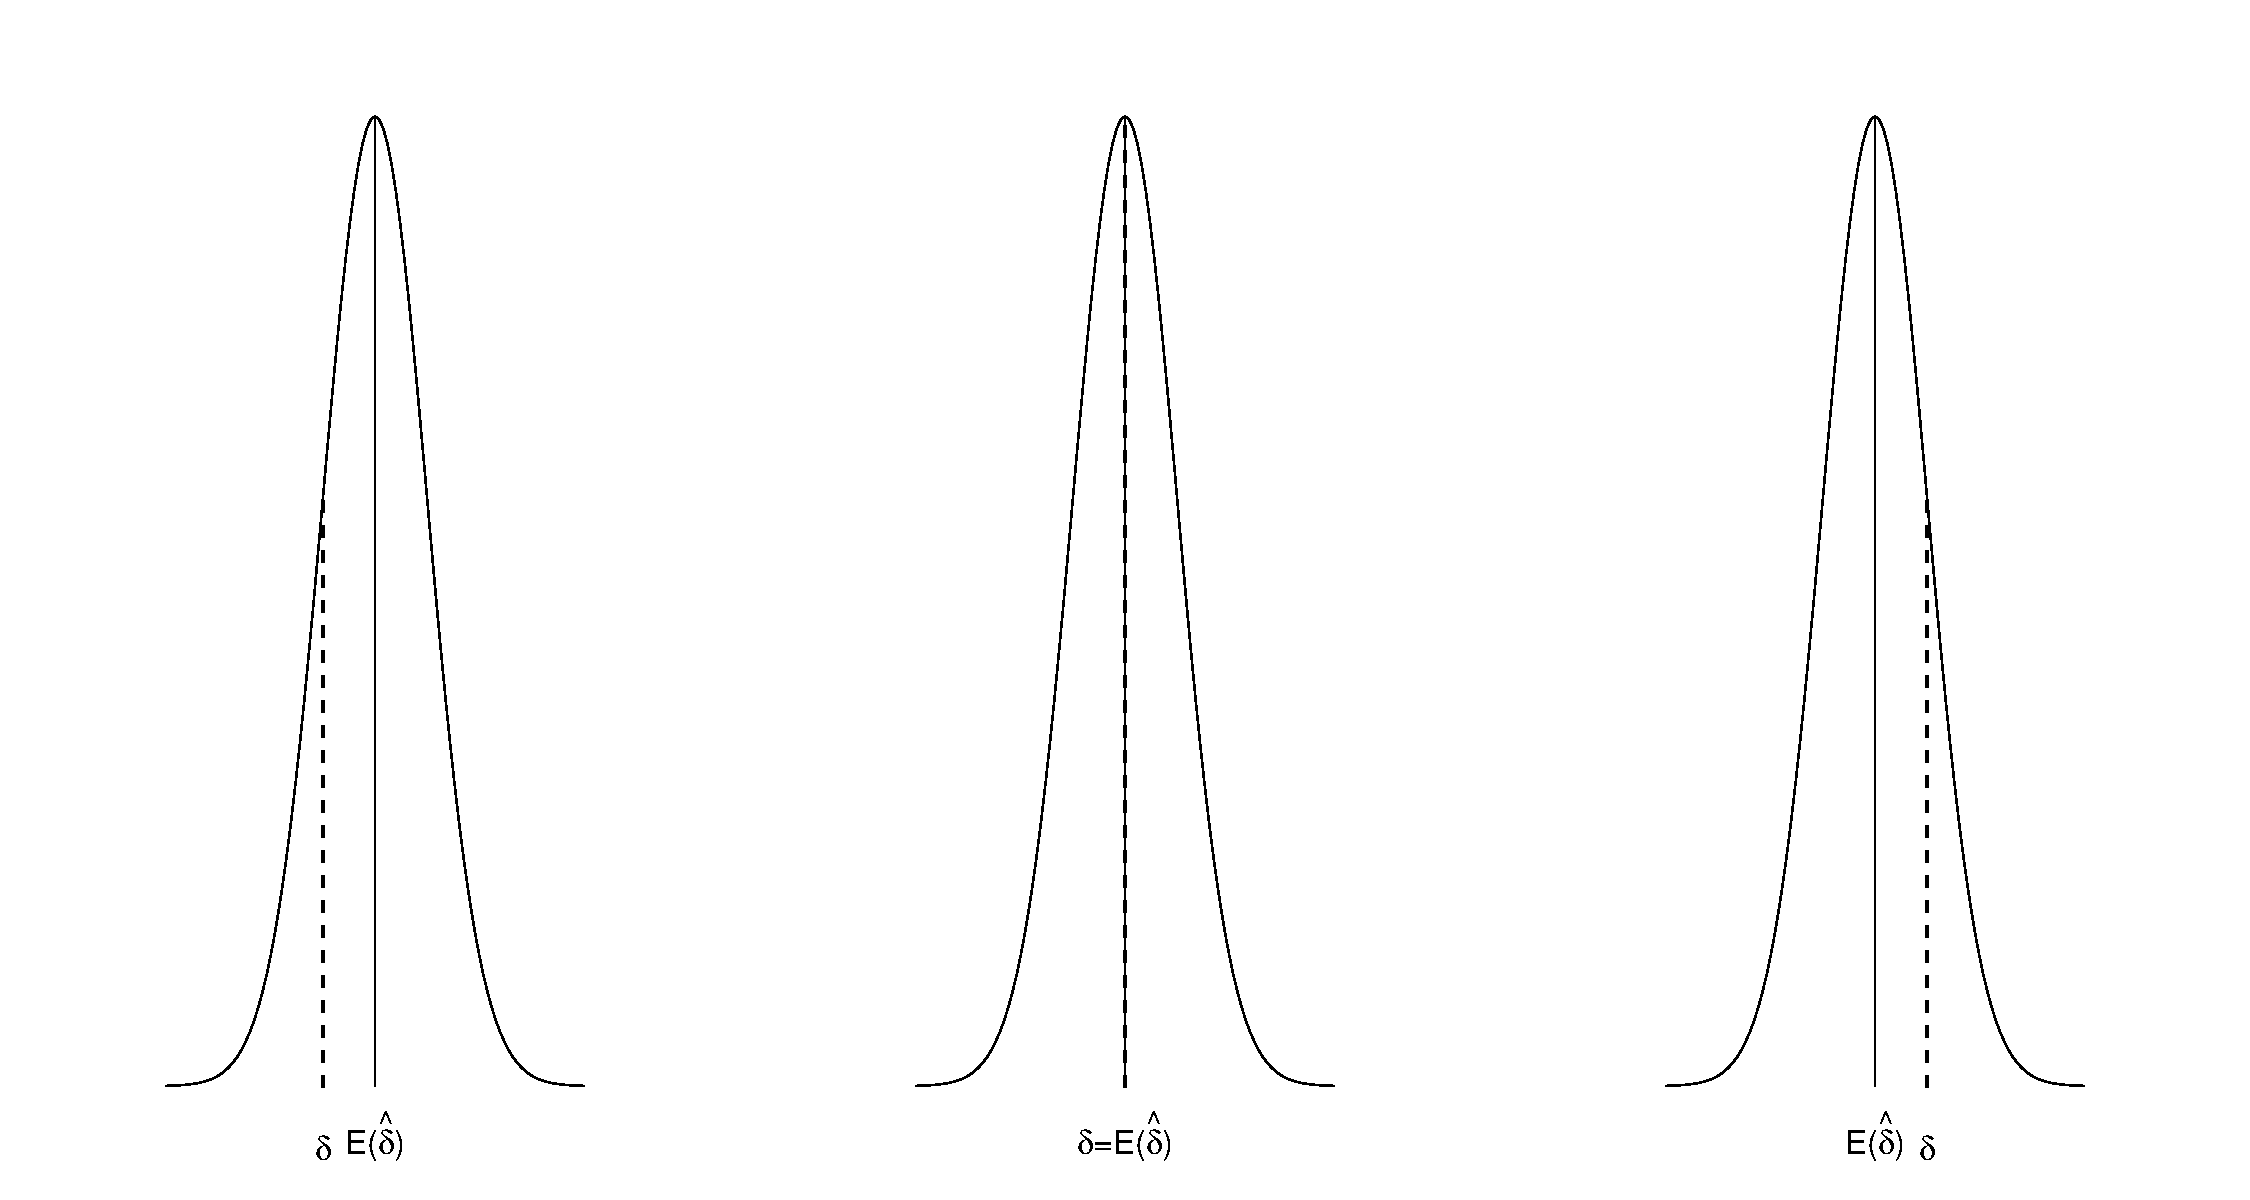
\includegraphics[width=400px]{template_files/figure-latex/BIAS-1} \caption{Sampling distribution for a positively biased (left), an unbiased (center) and a negatively biased estimator (right)}\label{fig:BIAS}
\end{figure}

As we can see in Tables 1 and 2 the bias is directly related to the
population effect size. The larger the population effect size, the
larger the bias. It is therefore also interesting to examine the
\emph{relative bias}, defined as the ratio between the bias and the
population effect size: \begin{equation} 
\delta_{relative \; bias}=\frac{E(\hat{\delta})-\delta}{\delta}
\label{eqn:RELBIAS}
\end{equation} While the bias informs us about the quality of estimates
on average, in particular their capacity of lying close to the true
value, it says nothing about individual estimates. Imagine a situation
where the distribution of estimates is centered around the real
parameter but with such a large variance that some point estimates are
very far from the center. This would be problematic, since any single
estimate might be very far from the true population value. Therefore it
is not only essential for an estimator to be unbiased, but it is also
desirable that the variability of its sampling distribution is small.
Ideally, sample estimates are close to the true population parameter.
Among two unbiased estimators \(\hat{\delta_1}\) and \(\hat{\delta_2}\),
we therefore say that \(\hat{\delta_1}\) is \emph{more efficient} than
\(\hat{\delta_2}\) if \begin{equation} 
Var(\hat{\delta}_1) \leq Var(\hat{\delta}_2)
\label{eqn:EFFICIENCY}
\end{equation} where \(Var(\hat{\delta})\) is the variance of the
sampling distribution of the estimator \(\hat{\delta}\). Among all
unbiased estimators, the more efficient estimator will be the one with
the smallest variance
\endnote{The Cramér-Rao inequality provides a theoretical lower bound for the variance of unbiased estimators. An estimator reaching this bound is therefore optimally efficient.}.
The variance of an estimator \(\hat{\delta}\) is a function of its size
(the larger the estimator, the larger the variance) and, therefore, we
might be interested in evaluating the \emph{relative variance} as the
ratio between the variance and the square of the population estimator:
\begin{equation} 
relative \; var(\hat{\delta}_1)=\frac{Var(\hat{\delta})}{\delta^2}
\label{eqn:RELVAR}
\end{equation} Note that both unbiasedness and efficiency are very
important when choosing an estimator. In some situations, it might be
better to have a slightly biased estimator with low variance, (so that
each estimate remains relatively close to the true parameter and one
might be able to apply bias correction techniques) rather than an
unbiased estimator with a large variance (Raviv, 2014).

Finally, the last property of a good point estimator is
\emph{consistency}. Consistency means that the bigger the sample size,
the closer the estimate is to the population parameter. In other words,
the estimates \emph{converge} to the true population parameter.

\hypertarget{different-measures-of-effect-sizes}{%
\subsection{Different measures of effect
sizes}\label{different-measures-of-effect-sizes}}

The \emph{d}-family effect sizes are commonly used for mean differences
between groups or conditions. The population effect size is defined as
\begin{equation} 
\delta = \frac{\mu_{1}-\mu_{2}}{\sigma} 
\label{eqn:Cohendelta}
\end{equation} where both populations follow a normal distribution with
mean \(\mu_j\) in the \(j^{th}\) population (\(j=1,2\)) and standard
deviation \(\sigma\). There exist different estimators of this effect
size measure. For all, the mean difference is estimated by the
difference \(\bar{X}_1-\bar{X}_2\) of both sample means. When the
equality of variances assumption is assumed, \(\sigma\) is estimated by
pooling both sample standard deviations (\(S_1\) and \(S_2\)). When the
equality of variances assumption cannot be assumed, alternatives to the
pooled standard deviation are available. In the next section we will
present effect sizes that assume equal variances between groups (Cohen's
\(d\) and Hedges' \(g\)), and effect sizes that do not assume equal
variances (Glass's \(d\), Shieh's \(d\), Cohen's \(d^*\), Glass's \(g\),
Shieh's \(g\), and Hedges' \(g^*\)). For each effect size we will
provide information about their theoretical bias, variance, and
consistency.

\hypertarget{when-variances-are-equal-between-groups}{%
\subsubsection{When variances are equal between
groups}\label{when-variances-are-equal-between-groups}}

When we have good reasons to assume equality of variances between groups
then the most common estimator of \(\delta\) is Cohen's \(d\), where the
sample mean difference is divided by a pooled error term (Cohen, 1965):
\begin{equation*} 
Cohen's \; d = \frac{\bar{X}_1-\bar{X}_2}{\sqrt{\frac{(n_1-1) \times S_1^2+(n_2-1) \times S_2^2}{n_1+n_2-2}}}
\label{eqn:Cohends}
\end{equation*} where \(S_j\) is the standard deviation, and \(n_j\) the
sample size of the \(j^{th}\) sample (\(j=1,2\)). The reasoning behind
this measure is to make use of the fact that both samples share the same
population variance (Keselman, Algina, Lix, Wilcox, \& Deering, 2008),
which means a more accurate estimation of the population variance can be
achieved by pooling both estimates of this parameter (i.e.~\(S_1\) and
\(S_2\)). Since the larger the sample size, the more accurate the
estimate, we give more weight to the estimate based on the larger sample
size. Cohen's \(d\) is directly related to Student's \emph{t}-statistic:
\begin{equation} 
t_{Student}=\frac{Cohen's \; d}{\sqrt{\frac{1}{n_1}+\frac{1}{n_2}}}\leftrightarrow Cohen's \; d =  t_{Student} \times \sqrt{\frac{1}{n_1}+\frac{1}{n_2}}
\label{eqn:Cohenvsstudent}
\end{equation} Under the assumption of normality and equal variances
between groups, Student's \emph{t}-statistic follows a
\emph{t}-distribution with known degrees of freedom \begin{equation} 
df_{Student} = n_1+n_2-2
\label{eqn:studentdf}
\end{equation} and noncentrality parameter
\endnote{Under the null hypothesis of no differences between sample means, Student's $t$-statistic will follow a central $t$-distribution with $n_1+n_2-2$ degrees of freedom. However, when the null hypothesis is false, the distribution of this quantity will not be centered, and a noncentral $t$-distribution will arise.}
\[ncp_{Student} = \frac{\delta_{Cohen}}{\sqrt{\frac{1}{n_1}+\frac{1}{n_2}}}\]
where \(\delta_{Cohen}= \frac{\mu_1-\mu_2}{\sigma_{pooled}}\) and
\(\sigma_{pooled}= \sqrt{\frac{(n_1-1) \times \sigma^2_1+(n_2-1) \times \sigma^2_2}{n_1+n_2-2}}\).
The relationship described in equation \ref{eqn:Cohenvsstudent} and the
theoretical distribution of Student's \emph{t}-statistic allow us to
determine the sampling distribution of Cohen's \(d\), and therefore, its
expectation and variance when the assumptions of normality and equal
variances are met. All these equations are provided in Table 1. For
interested readers, Supplemental Material 1 provides a detailed
examination of the theoretical bias and variance of Cohen's \(d\) based
on Table 1, as well as the bias and variance of all other estimators
described later, based on Tables 2 and 3, with the goal to determine
which parameters influence the bias and variance of different
estimators. The main results will be discussed in the section ``Monte
Carlo Simulations: assessing the bias, efficiency and consistency of 5
estimators'' below.

While Cohen's \(d\) is a consistent estimator, its bias and variance are
substantial with small sample sizes, even under the assumptions of
normality and equal variances (Lakens, 2013). In order to compensate for
Cohen's \(d\) bias with small sample sizes, Hedges \& Olkin (1985)
defined a bias-corrected version: \begin{equation*} 
Hedges' \; g = Cohen's \; d \times \frac{\Gamma(\frac{df_{Student}}{2})}{\sqrt{\frac{df_{Student}}{2}} \times \Gamma(\frac{df_{Student}-1}{2})}
\label{eqn:Hedgesgs}
\end{equation*} where \(df_{Student}\) has been defined in equation
\ref{eqn:studentdf} and \(\Gamma()\) is the gamma function (for
integers, \(\Gamma(x)\) is the factorial of \(x\) minus \(1\):
\(\Gamma(x)=(x-1)!\), Goulet-Pelletier \& Cousineau, 2018). This
equation can be approximated as follows: \begin{equation*} 
Hedges' \; g = Cohen's \; d \times \left( 1- \frac{3}{4N -9} \right)
\label{eqn:Hedgesgsapprox}
\end{equation*} where \(N\) is the total sample size. Hedges' \(g\) is
theoretically unbiased when the assumptions of normality and equal
variances are met (see Table 1). Moreover, while the variance of both
Cohen's \(d\) and Hedges' \(g\) depend on the same parameters (i.e.~the
total sample size (N) and the sample sizes ratio
\(\left(\frac{n_2}{n_1}\right)\)), Hedges' \(g\) is less variable,
especially with small sample sizes
\endnote{In Table 1, one can see that the variance of Hedges' $g$ equals the variance of Cohen's $d$, multiplied by $\left[\frac{\Gamma(\frac{df}{2})}{\sqrt{\frac{df}{2}} \times \Gamma(\frac{df-1}{2})} \right] ^2$. This term is always less than 1 and tends to 1 when the sample sizes tends to infinity ($52 \le \left[\frac{\Gamma(\frac{df}{2})}{\sqrt{\frac{df}{2}} \times \Gamma(\frac{df-1}{2})} \right] ^2 < 1$ for $3 \le df < \infty$). As a consequence, the larger the total sample size, the smaller the difference between the variance of Cohen's $d$ and Hedges' $g$.}.

While the pooled error term is the best choice when variances are equal
between groups (Grissom \& Kim, 2001), it may not be well advised for
use with data that violate this assumption (Cumming, 2013~; Grissom \&
Kim, 2001, 2005~; Kelley, 2005~; Shieh, 2013). When variances are
unequal between groups, the expression in equation 5 is no longer valid
because both groups do not share a common population variance. If we
pool the estimates of two unequal population variances, the estimator of
effect size will be smaller as it should be in case of positive pairing
(i.e.~the group with the larger sample size is extracted from the
population with the larger variance) and larger as it should be in case
of negative pairing (i.e.~the group with the larger sample size is
extracted from the population with the smaller variance). Because the
assumption of equal variances across populations is rarely realistic in
practice (Cain, Zhang, \& Yuan, 2017~; Delacre, Lakens, \& Leys, 2017~;
Delacre, Leys, Mora, \& Lakens, 2019~; Erceg-Hurn \& Mirosevich, 2008~;
Glass, Peckham, \& Sanders, 1972~; Grissom, 2000~; Micceri, 1989~; Yuan,
Bentler, \& Chan, 2004), both Cohen's \(d\) and Hedges' \(g\) should be
abandoned in favor of an alternative robust to unequal population
variances.

\newpage
\begin{landscape}

\begin{longtable}[]{@{}
  >{\raggedright\arraybackslash}p{(\columnwidth - 6\tabcolsep) * \real{0.13}}
  >{\centering\arraybackslash}p{(\columnwidth - 6\tabcolsep) * \real{0.12}}
  >{\centering\arraybackslash}p{(\columnwidth - 6\tabcolsep) * \real{0.27}}
  >{\centering\arraybackslash}p{(\columnwidth - 6\tabcolsep) * \real{0.48}}@{}}
\caption{Expectation, bias and variance of Cohen's \(d\) and Hedges'
\(g\) under the assumptions that independent residuals are normally
distributed with equal variances across groups.}\tabularnewline
\toprule
& df & Expectation & Variance \\
\midrule
\endfirsthead
\toprule
& df & Expectation & Variance \\
\midrule
\endhead
Cohen's \(d\) & \(N-2\) & \(\delta_{Cohen} \times c_f\) &
\(\frac{N\times df}{n_1n_2 \times (df-2)} + \delta^2_{Cohen} \left[ \frac{df}{df-2} - c_f^2\right]\) \\
& & & \\
& & \(\approx \frac{\delta_{Cohen}}{\left(1-\frac{3}{4N-9}\right)}\) &
\(\approx \frac{N\times df}{n_1n_2 \times (df-2)} + \delta^2_{Cohen} \left[ \frac{df}{df-2} - \left( \frac{1}{1-\frac{3}{4N-9} }\right)^2\right]\) \\
& & & \\
& & & \\
Hedges' \(g\) & \(N-2\) & \(\delta_{Cohen}\) &
\(Var(Cohen's \; d) \times \left[ \frac{\Gamma(\frac{df}{2})}{\sqrt{\frac{df}{2}} \times \Gamma(\frac{df-1}{2})} \right]^2\) \\
& & & \\
& & &
\(\approx Var(Cohen's \; d) \times \left[1-\frac{3}{4N-9}\right]^2\) \\
& & & \\
\bottomrule
\end{longtable}

\emph{Note}. \(\delta_{Cohen}= \frac{\mu_1-\mu_2}{\sigma_{pooled}}\) and
\(c_f=\frac{\sqrt{\frac{df}{2}} \times \Gamma\left( \frac{df-1}{2}\right)}{\Gamma\left( \frac{df}{2}\right)}\);
Cohen's \(d\) is a biased estimator, because its expectation differs
from the population effect size. Moreover, the larger the population
estimator (\(\delta_{Cohen}\)), the larger the bias. Indeed, the bias is
the difference between the expectation and \(\delta_{Cohen}\):
\(\delta_{bias} = \delta_{Cohen} \times (c_f-1)\). On the other hand,
Hedges' \(g\) is an unbiased estimator, because its expectation equals
\(\delta_{Cohen}\); equations in Table 1 require \(df \ge 3\)
(i.e.~\(N \ge 5\)).

\end{landscape}

\hypertarget{when-variances-are-unequal-between-populations}{%
\subsubsection{When variances are unequal between
populations}\label{when-variances-are-unequal-between-populations}}

In his review, Shieh (2013) mentions three options available in the
literature to deal with the case of unequal variances: (A) the Glass's
\(d\), (B) the Shieh's \(d\) and (C) the Cohen's \(d^*\).

\hypertarget{glasss-bmd}{%
\paragraph{\texorpdfstring{Glass's
\(\bm{d}\)}{Glass's \textbackslash bm\{d\}}}\label{glasss-bmd}}

When comparing one control group with one experimental group, Glass,
McGav, \& Smith (1981) recommend using the standard deviation of the
control group as standardizer. This yields \begin{equation*} 
Glass's \; d = \frac{\bar{X}_{e} - \bar{X}_{c}}{S_{c}}
\label{eqn:Glassds}
\end{equation*} where \(\bar{X}_{e} \; and \; \bar{X}_{c}\) are the
sample means of the experimental and control groups, and \(S_{c}\) is
the sample SD of the control group. One argument in favour of using
\(S_c\) as standardizer is the fact that it is not affected by the
experimental treatment. When it is easy to identify which group is the
``control'' one, it is therefore convenient to compare the effect size
estimation of different designs studying the same effect (Cumming,
2013). However, defining this group is not always obvious (Coe, 2002).
This could induce large ambiguity because depending on the chosen \(SD\)
as standardizer, measures could be substantially different (Shieh,
2013). The distribution of Glass's \(d\) is defined as in Algina,
Keselman, \& Penfield (2006): \begin{equation} 
Glass's \; d \sim \sqrt{\frac{1}{n_{c}}+\frac{\sigma_{e}^2}{n_{e} \times \sigma^2_{c}}} \times t_{df,ncp}
\label{eqn:glassvst}
\end{equation} where \(n_c\) and \(n_e\) are the sample sizes of the
control and experimental groups, and \(df\) and \(ncp\) are defined as
follows: \begin{equation} 
df = n_{c}-1
\label{eqn:glassdf}
\end{equation} \begin{equation*} 
ncp = \frac{\delta_{Glass}}{\sqrt{\frac{1}{n_{c}} + \frac{\sigma_{e}^2}{n_{e} \times \sigma^2_{c}}}}
\label{eqn:glassncp}
\end{equation*} where
\(\delta_{Glass} = \frac{\mu_{c}-\mu_{e}}{\sigma_{c}}\) and \(\mu_c\)
and \(\mu_e\) are respectively the mean of the populations control and
experimental groups are extracted from. Thanks to equation
\ref{eqn:glassvst}, we can compute its theoretical expectation and
variance when the assumption of normality is met (see Table 2), and
therefore determine which factors influence bias and variance, and how
they do so (see Supplemental Material 1).

\newpage
\begin{landscape}

\begin{longtable}[]{@{}
  >{\raggedright\arraybackslash}p{(\columnwidth - 6\tabcolsep) * \real{0.11}}
  >{\centering\arraybackslash}p{(\columnwidth - 6\tabcolsep) * \real{0.20}}
  >{\centering\arraybackslash}p{(\columnwidth - 6\tabcolsep) * \real{0.18}}
  >{\centering\arraybackslash}p{(\columnwidth - 6\tabcolsep) * \real{0.51}}@{}}
\caption{Expectation, bias and variance of Glass's \(d\), Cohen's
\(d^*\) and Shieh's \(d\) under the assumption that independent
residuals are normally distributed.}\tabularnewline
\toprule
& df & Expectation & Variance \\
\midrule
\endfirsthead
\toprule
& df & Expectation & Variance \\
\midrule
\endhead
Glass's \(d\) & \(n_c-1\) & ~\(\delta_{Glass} \times c_f\) &
\(\frac{df}{df-2} \times \left( \frac{1}{n_c} + \frac{\sigma^2_e}{n_e\sigma^2_c}\right) + \delta^2_{Glass} \left( \frac{df}{df-2} - c_f^2 \right)\) \\
& & & \\
Cohen's \(d^*\) &
\(\frac{(n_1-1)(n_2-1)(\sigma^2_1+\sigma^2_2)^2}{(n_2-1)\sigma^4_1+(n_1-1)\sigma^4_2}\)
& \(\delta^*_{Cohen} \times c_f\) &
\(\frac{df}{df-2} \times \frac{2\left( \frac{\sigma^2_1}{n_1} + \frac{\sigma^2_2}{n_2} \right)}{\sigma^2_1+\sigma^2_2} + (\delta^*_{Cohen})^2 \left( \frac{df}{df-2} - c_f^2 \right)\) \\
& & & \\
& & \(\approx \delta^*_{Cohen} \times \frac{4df-1}{4(df-1)}\) &
\(\approx \frac{df}{df-2} \times \frac{2\left( \frac{\sigma^2_1}{n_1} + \frac{\sigma^2_2}{n_2} \right)}{\sigma^2_1+\sigma^2_2} + (\delta^*_{Cohen})^2 \left[ \frac{df}{df-2} - \left( \frac{4 \;df-1}{4(df-1)}\right)^2 \right]\) \\
& & & \\
Shieh's \(d\) &
\(\frac{\left(\frac{\sigma^2_1}{n_1}+\frac{\sigma^2_2}{n_2} \right)^2}{\frac{(\sigma^2_1/n_1)^2}{n_1-1}+\frac{(\sigma^2_2/n_2)^2}{n_2-1}}\)
& \(\delta_{Shieh} \times c_f\) &
\(\frac{df}{(df-2)N} + \delta^2_{Shieh} \left( \frac{df}{df-2} - c_f^2 \right)\) \\
& & & \\
\bottomrule
\end{longtable}

\emph{Note}.
\(c_f=\frac{\sqrt{\frac{df}{2}} \times \Gamma\left( \frac{df-1}{2}\right)}{\Gamma\left( \frac{df}{2}\right)}\);
\(\delta_{Glass}=\frac{\mu_c-\mu_e}{\sigma_c}\),
\(\delta_{Shieh}=\frac{\mu_1-\mu_2}{\sqrt{\frac{\sigma^2_1}{n_1/N}+\frac{\sigma^2_2}{n_2/N}}}\)
and
\(\delta^*_{Cohen}=\frac{\mu_1-\mu_2}{\sqrt{\frac{\sigma^2_1+\sigma^2_2}{2}}}\);
all estimators are biased estimators, because their expectations differ
from the population effect size \(\delta\). Moreover, the larger the
population estimator (\(\delta\)), the larger the bias. Indeed, the bias
is the difference between the expectation and \(\delta\):
\(\delta_{bias} = \delta \times (c_f-1)\). Equations require
\(df \ge 3\) and at least 2 subjects per group.

\end{landscape}
\newpage

\hypertarget{shiehs-bmd}{%
\paragraph{\texorpdfstring{Shieh's
\(\bm{d}\)}{Shieh's \textbackslash bm\{d\}}}\label{shiehs-bmd}}

Kulinskaya \& Staudte (2007) were the first to recommend the use of a
standardizer that takes the sample sizes allocation ratios into account,
in addition to the variance of both samples. Shieh (2013), following
Kulinskaya \& Staudte (2007), proposed a modification of the exact
\emph{SD} of the sample mean difference: \begin{equation*} 
Shieh's \; d = \frac{\bar{X}_1 - \bar{X}_2}{\sqrt{S_1^2/q_1+S_2^2/q_2}}; \;\;\; q_j=\frac{n_j}{N} (j=1,2)
\label{eqn:Shiehds}
\end{equation*} where \(N = n_1+n_2\). Shieh's \(d\) is directly related
with Welch's \emph{t}-statistic: \begin{equation} 
Shieh's \; d=\frac{t_{Welch}}{\sqrt{N}}\leftrightarrow t_{welch} = Shieh's \; d \times \sqrt{N}
\label{eqn:shiehvswelch}
\end{equation} The exact distribution of Welch's \emph{t}-statistic is
more complicated than the exact distribution of Student's
\emph{t}-statistic, but it can be approximated, under the assumption of
normality, by a \emph{t}-distribution with degrees of freedom and
noncentrality parameters (Shieh, 2013~; Welch, 1938): \begin{equation} 
df_{Welch} = \frac{\left(\frac{\sigma^2_1}{n_1}+\frac{\sigma^2_2}{n_2} \right)^2}{\frac{(\sigma^2_1/n_1)^2}{n_1-1}+\frac{(\sigma^2_2/n_2)^2}{n_2-1}}
\label{eqn:welchdf}
\end{equation} \begin{equation*} 
ncp_{Welch} = \delta_{Shieh} \times \sqrt{N} = \frac{\mu_1-\mu_2}{\sqrt{\frac{\sigma_1^2}{n1}+\frac{\sigma_2^2}{n_2}}}
\label{eqn:welchncp}
\end{equation*} where
\(\delta_{Shieh}=\frac{\mu_1-\mu_2}{\sqrt{\frac{\sigma_1^2}{n_1/N}+\frac{\sigma_2^2}{n_2/N}}}\).
The relationship described in equation \ref{eqn:shiehvswelch} and the
theoretical distribution of Welch's \emph{t}-statistic allow us to
approximate the sampling distribution of Shieh's \(d\). Based on the
sampling distribution of Shieh's \(d\), we can estimate its theoretical
expectation and variance under the assumption of normality (see Table
2), and thereby determine which factors influence bias and variance, and
how they do so (see Supplemental Material 1).

As demonstrated in the Appendix, when variances and sample sizes are
equal across groups, the biases and variances of Cohen's \(d\) and
Shieh's \(d\) are identical except for multiplication by a constant. The
same is true for the estimators \(\delta_{Cohen}\) and
\(\delta_{Shieh}\):\\
\begin{equation} 
\delta_{Cohen} = 2 \times \delta_{Shieh} \quad (\mbox{considering} \; \sigma_1 = \sigma_2 \; \mbox{and} \; n_1 = n_2)
\label{eqn:CohenShieh}
\end{equation} \begin{equation} 
Bias_{Cohen's \; d} = 2 \times Bias_{Shieh's \; d} \quad (\mbox{considering} \; \sigma_1 = \sigma_2 \; \mbox{and} \; n_1 = n_2)
\label{eqn:biasCohenshieh}
\end{equation} \begin{equation} 
Var_{Cohen's \; d} = 4 \times Var_{Shieh's \; d} \quad (\mbox{considering}\; \sigma_1 = \sigma_2 \; \mbox{and} \; n_1 = n_2)
\label{eqn:varCohenshieh}
\end{equation} We can deduce from equations \ref{eqn:CohenShieh},
\ref{eqn:biasCohenshieh} and \ref{eqn:varCohenshieh} that relative to
their respective population effect size, Cohen's \(d\) and Shieh's \(d\)
are equally accurate. In other words, their relative bias and variance
are identical. This is a good illustration of our motivation to favor
relative bias and variance (previously defined in equations
\ref{eqn:RELBIAS} and \ref{eqn:RELVAR}) over the most commonly used raw
bias and variance (previously defined in equations \ref{eqn:BIAS} and
\ref{eqn:EFFICIENCY}).

When sample sizes are not equal, according to the statistical properties
of Welch's statistic under heteroscedasticity, Shieh's \(d\) accounts
for the allocation ratio of sample sizes to each condition. The lack of
generality caused by taking this specificity of the design into account
has led Cumming (2013) to question its usefulness in terms of
interpretability: when the mean difference (\(\bar{X_1}-\bar{X_2}\)),
\(S_1\), and \(S_2\) remain constant, Shieh's \(d\) will vary as a
function of the sample sizes allocation ratio (unlike Cohen's \(d^*\)
that we will define below). At the population level, \(\delta_{Shieh}\)
also depends on the sample sizes allocation ratio, as illustrated in the
following shiny application:
\url{https://effectsize.shinyapps.io/ShiehvsCohen/}.

\hypertarget{cohens-bmd}{%
\paragraph{\texorpdfstring{Cohen's
\(\bm{d^*}\)}{Cohen's \textbackslash bm\{d\^{}*\}}}\label{cohens-bmd}}

An effect size estimator based on the sample mean difference divided by
the square root of the non pooled average of both variance estimates was
suggested by Welch (1938). Here, we indicate the difference between
Cohen's \(d\) (based on the pooled standard deviations) and Cohen's
\(d^*\) with an asterisk. This yields: \begin{equation*} 
Cohen's \; d^* = \frac{\bar{X}_{1} - \bar{X}_{2}}{ \sqrt{\frac{\left(S^2_{1}+S^2_{2} \right)}{2}}}
\label{eqn:Cohenprimeds}
\end{equation*} where \(\bar{X}_{j}\) is the mean and \(S_j\) is the
standard deviation of the \(j^{th}\) sample (j = 1,2). We know the
distribution of Cohen's \(d^*\) (Huynh, 1989): \begin{equation} 
Cohen's \; d^* \sim  \sqrt{\frac{2(n_2\times\sigma^2_1+n_1\times\sigma^2_2)}{n_1n_2(\sigma^2_1+\sigma^2_2)}} \times t_{df^*,ncp^*}
\label{eqn:Cohendprimedist}
\end{equation} Where \(df^*\) and \(ncp^*\) are defined as follows:
\begin{equation} 
df^* = \frac{(n_1-1)(n_2-1)(\sigma^2_1+\sigma^2_2)^2}{(n_2-1)\sigma^4_1+(n_1-1)\sigma^4_2}
\label{eqn:Cohendprimedf}
\end{equation} \begin{equation*} 
ncp^*=\delta^*_{Cohen} \times \sqrt{\frac{n_1n_2(\sigma^2_1+\sigma^2_2)}{2(n_2\sigma^2_1+n_1\sigma^2_2)}}=\frac{\mu_1-\mu_2}{\sqrt{\frac{\sigma_1^2}{n_1}+\frac{\sigma^2_2}{n_2}}}
\label{eqn:Cohendprimevst}
\end{equation*} where
\(\delta^*_{Cohen}=\frac{\mu_1-\mu_2}{\sqrt{\frac{\sigma^2_1+\sigma^2_2}{2}}}\).
Using equation \ref{eqn:Cohendprimedist} we can compute its theoretical
expectation and variance when the assumption of normality is met (see
Table 2), and therefore determine which factors influence bias and
variance, and how they do so (see Supplemental Material 1). This
estimator has been widely criticized, because it results in a variance
term of an artificial population (i.e.~since the variance term does not
estimate the variance of one or the other group, the composite variance
is an estimation of the variance of an artificial population) and is
therefore very difficult to interpret (Grissom \& Kim, 2001), and unless
both sample sizes are equal, the variance term does not correspond to
the variance of the mean difference (Shieh, 2013).

However, we will show throughout the simulation section that this
estimator exhibits very good inferential properties. Moreover, it has a
constant value across sample sizes ratios, as shown in the Shiny App at
\url{https://effectsize.shinyapps.io/ShiehvsCohen/}.

\hypertarget{glasss-bmg-shiehs-bmg-and-hedges-bmg}{%
\paragraph{\texorpdfstring{Glass's \(\bm{g}\), Shieh's \(\bm{g}\) and
Hedges'
\(\bm{g^*}\)}{Glass's \textbackslash bm\{g\}, Shieh's \textbackslash bm\{g\} and Hedges' \textbackslash bm\{g\^{}*\}}}\label{glasss-bmg-shiehs-bmg-and-hedges-bmg}}

As for Cohen's \(d\), a Hedges' correction can be applied in order to
compensate for the bias of Glass's \(d\), Shieh's \(d\) and Cohen's
\(d^*\) with small sample sizes (see Table 2). This correction has the
following general form: \begin{equation*} 
g = d \times \frac{\Gamma(\frac{\nu}{2})}{\sqrt{\frac{\nu}{2}} \times \Gamma(\frac{\nu-1}{2})}
\end{equation*} where the distinct values of \(\nu\) are provided in
equation \ref{eqn:glassdf} for Glass's \(g\), in equation
\ref{eqn:Cohendprimedf} for Hedges' \(g^*\) and in equation
\ref{eqn:welchdf} for Shieh's \(g\). The three corrected estimators are
theoretically unbiased when the assumption of normality is met. Their
variance is a function of the same parameters as their biased
equivalent. However, due to the correction they have a smaller variance,
especially with small sample sizes, as shown in Table 3. In summary:

\begin{itemize}
\tightlist
\item
  The variances of Hedges' \(g^*\) and Shieh's \(g\) depend on the total
  sample size (\(N\)), their respective population effect size
  (\(\delta\)), and the interaction between the sample sizes ratio and
  the \(SD\)-ratio
  \(\left(\frac{n_2}{n_1}\times\frac{\sigma_2}{\sigma_1} \right)\).\\
\item
  The variance of Glass's \(g\) also depends on \(N\), \(\delta\) and
  \(\frac{n_c}{n_e}\times\frac{\sigma_c}{\sigma_e}\). In addition, there
  is also a main effect of the \(SD\)-ratio
  \(\left(\frac{\sigma_c}{\sigma_e} \right)\) on its variance.
\end{itemize}

How these parameters influence the variance of the estimators will be
summarized and illustrated in Monte Carlo simulations below.

\newpage
\begin{landscape}

\begin{longtable}[]{@{}
  >{\raggedright\arraybackslash}p{(\columnwidth - 6\tabcolsep) * \real{0.11}}
  >{\centering\arraybackslash}p{(\columnwidth - 6\tabcolsep) * \real{0.20}}
  >{\centering\arraybackslash}p{(\columnwidth - 6\tabcolsep) * \real{0.18}}
  >{\centering\arraybackslash}p{(\columnwidth - 6\tabcolsep) * \real{0.51}}@{}}
\caption{Expectation, bias and variance of Glass's \(g\), Hedges'
\(g^*\) and Shieh's \(g\) under the assumption that independent
residuals are normally distributed.}\tabularnewline
\toprule
& df & Expectation & Variance \\
\midrule
\endfirsthead
\toprule
& df & Expectation & Variance \\
\midrule
\endhead
Glass's \(g\) & \(n_c-1\) & ~\(\delta_{glass}\) &
\(Var(Glass's \; d) \times \left( \frac{\Gamma\left(\frac{df}{2} \right)}{\sqrt{\frac{df}{2}} \times \Gamma \left( \frac{df-1}{2}\right)}\right)^2\) \\
& & & \\
Hedges' \(g^*\) &
\(\frac{(n_1-1)(n_2-1)(\sigma^2_1+\sigma^2_2)^2}{(n_2-1)\sigma^4_1+(n_1-1)\sigma^4_2}\)
& \(\delta^*_{Cohen}\) &
\(Var(Cohen's \; d^*) \times \left( \frac{\Gamma\left(\frac{df}{2} \right)}{\sqrt{\frac{df}{2}} \times \Gamma \left( \frac{df-1}{2}\right)}\right)^2\) \\
& & & \\
Shieh's \(g\) &
\(\approx \frac{\left(\frac{\sigma^2_1}{n_1}+\frac{\sigma^2_2}{n_2} \right)^2}{\frac{(\sigma^2_1/n_1)^2}{n_1-1}+\frac{(\sigma^2_2/n_2)^2}{n_2-1}}\)
& \(\delta_{Shieh}\) &
\(Var(Shieh's \; d) \times \left( \frac{\Gamma\left(\frac{df}{2} \right)}{\sqrt{\frac{df}{2}} \times \Gamma \left( \frac{df-1}{2}\right)}\right)^2\) \\
& & & \\
\bottomrule
\end{longtable}

\emph{Note}.
\(c_f=\frac{\sqrt{\frac{df}{2}} \times \Gamma\left( \frac{df-1}{2}\right)}{\Gamma\left( \frac{df}{2}\right)}\);
\(\delta_{Glass}=\frac{\mu_c-\mu_e}{\sigma_c}\),
\(\delta_{Shieh}=\frac{\mu_1-\mu_2}{\sqrt{\frac{\sigma^2_1}{n_1/N}+\frac{\sigma^2_2}{n_2/N}}}\)
and
\(\delta^*_{Cohen}=\frac{\mu_1-\mu_2}{\sqrt{\frac{\sigma^2_1+\sigma^2_2}{2}}}\);
all estimators are unbiased estimators, because their expectations equal
the population effect size \(\delta\); equations require \(df \ge 3\)
and at least 2 subjects per group.

\end{landscape}
\newpage

\hypertarget{monte-carlo-simulations}{%
\subsubsection{Monte Carlo Simulations}\label{monte-carlo-simulations}}

\hypertarget{assessing-the-bias-efficiency-and-consistency-of-5-estimators}{%
\paragraph{Assessing the bias, efficiency and consistency of 5
estimators}\label{assessing-the-bias-efficiency-and-consistency-of-5-estimators}}

\hypertarget{method}{%
\subparagraph{Method}\label{method}}

We performed Monte Carlo simulations using R (version 3.5.0) to assess
the bias, efficiency and consistency of Hedges \(g\), Glass's \(g\)
(using respectively the sample \(SD\) of the first or second group as a
standardizer), Hedges' \(g^*\) and Shieh's \(g\).

A set of 100,000 datasets was generated for 1,008 scenarios as a
function of different criteria. In 252 scenarios, samples were extracted
from a normally distributed population (in order to ensure the
reliability of our calculation method) and in 756 scenarios, samples
were extracted from non normal population distributions. In order to
assess the quality of estimators under realistic deviations from the
normality assumption, we referred to the review of Cain, Zhang, \& Yuan
(2017). Cain, Zhang, \& Yuan (2017) investigated 1,567 univariate
distributions from 194 studies published by authors in Psychological
Science (from January 2013 to June 2014) and the American Education
Research Journal (from January 2010 to June 2014). For each
distribution, they computed Fisher's skewness
\[G_{1}=\frac{\sqrt{n(n-1)}}{n-2} \frac{m_{3}}{\sqrt{(m_{2})^3}}\] and
kurtosis
\[G_{2}=\frac{n-1}{(n-2)(n-3)}\times \left[(n+1)\left(\frac{m_{4}}{(m_{2})^2}-3\right)+6\right]\]
where \(n\) is the sample size and \(m_{2}\), \(m_{3}\) and \(m_{4}\)
are respectively the second, third and fourth centered moments. They
found values of kurtosis from \(G_2\) = -2.20 to 1,093.48. According to
their suggestions, throughout our simulations, we kept constant the
population kurtosis value at the 99th percentile of their distribution
of kurtosis, i.e.~\(G_2\)=95.75. Regarding skewness, we simulated
population parameter values which correspond to the 1st and 99th
percentile of their distribution of skewness, i.e.~respectively \(G_1\)
= -2.08 and \(G_1\) = 6.32. We also simulated samples extracted from
population where \(G_1\) = 0, in order to assess the main effect of high
kurtosis on the quality of estimators. All possible combinations of
population skewness and kurtosis and the number of scenarios for each
combination are summarized in Table 4.

\begin{longtable}[]{@{}ccccc@{}}
\caption{Number of combinations of skewness and kurtosis in our
simulations.}\tabularnewline
\toprule
& & & \textbf{Kurtosis} & \\
\midrule
\endfirsthead
\toprule
& & & \textbf{Kurtosis} & \\
\midrule
\endhead
& & 0 & 95.75 & \textbf{TOTAL} \\
& & --------------- & -------------- & --------------- \\
& 0 & 252 & 252 & \textbf{504} \\
& & & & \\
\textbf{Skewness} & -2.08 & / & 252 & \textbf{252} \\
& & & & \\
& 6.32 & / & 252 & \textbf{252} \\
& & & & \\
& \textbf{TOTAL} & \textbf{252} & \textbf{756} & \textbf{1008} \\
\bottomrule
\end{longtable}

\emph{Note.} Fisher's skewness (\(G_1\)) and kurtosis (\(G_2\)) are
presented in Table 4. The 252 combinations where both \(G_1\) and
\(G_2\) equal 0 correspond to the normal case.

For the 4 resulting combinations of skewness and kurtosis (see Table 4),
all other parameter values were chosen in order to illustrate the
consequences of factors identified as playing a key role on the variance
of unbiased estimators. We manipulated the population mean difference
(\(\mu_1-\mu_2\)), the sample sizes (\emph{n}), the sample size ratio
(\emph{n}-ratio = \(\frac{n_2}{n_1}\)), the population \emph{SD}-ratio
(i.e.~\(\frac{\sigma_2}{\sigma_1}\)), and the sample size and population
variance pairing
\(\left(\frac{n_2}{n_1}\times\frac{\sigma_2}{\sigma_1} \right)\). In our
scenarios, \(\mu_2\) was always 0 and \(\mu_1\) varied from 1 to 4, in
steps of 1 (so does
\(\mu_1-\mu_2\))\endnote{In the original plan, we had added 252 simulations in which $\mu_1$ and $\mu_2$ were both null. We decided not to present the results of these simulations in the main article, because the relative bias and the relative variance appeared to us to be very useful to fully understand the comparison of the estimators, and computing them is impossible when the real mean difference is zero. Indeed, for these specific configurations, both relative bias and relative variance would have infinite values due to the presence of the population effect size term in their denominator. However, these extra simulations were included in the simulation checks, in Supplemental Material 2. }.
Moreover, \(\sigma_1\) always equals 1, and \(\sigma_2\) equals .1, .25,
.5, 1, 2, 4 or 10, and therefore, the \(SD\)-ratio were 10, 4, 2, 1, .5,
.25 or .1. The simulations for which both \(\sigma_1\) and \(\sigma_2\)
equal 1 are the particular case of homoscedasticity, or equal population
variances across groups. The sample sizes of both groups (\(n_1\) and
\(n_2\)) were 20, 50 or 100. When sample sizes of both groups are equal,
the \emph{n}-ratio equals 1 (this is known as a balanced design). All
possible combinations of \emph{n}-ratio and population \emph{SD}-ratio
were simulated in order to distinguish scenarios where both sample sizes
and population variances are unequal across groups (with positive
pairing when the group with the largest sample size is extracted from
the population with the largest \emph{SD}, and negative pairing when the
group with the smallest sample size is extracted from the population
with the smallest \emph{SD}) and scenarios with no pairing between
sample sizes and variances (sample sizes and/or population \emph{SD} are
equal across all groups). In sum, the simulations grouped over different
sample sizes yield 4 conditions (a, b, c and d) based on the
\emph{n}-ratio, population \emph{SD}-ratio, and sample size and
population variance pairing, as summarized in Table 5. We chose to
divide scenarios into these 4 conditions because analyses in
Supplemental Material 1 revealed main and interaction effects of sample
sizes ratio and \(SD\)-ratio on the bias and variance of some
estimators.

\begin{longtable}[]{@{}ccccc@{}}
\caption{4 conditions based on the \(n\)-ratio and the
\(SD\)-ratio.}\tabularnewline
\toprule
& & & \textbf{\emph{n}-ratio} & \\
\midrule
\endfirsthead
\toprule
& & & \textbf{\emph{n}-ratio} & \\
\midrule
\endhead
& & \textbf{1} & \textbf{\textgreater1} & \textbf{\textless1} \\
& & ------------ & ------------- & ------------- \\
& \textbf{1} & a & b & b \\
& & & & \\
\textbf{\emph{SD}-ratio} & \textbf{\textgreater1} & c & d & d \\
& & & & \\
& \textbf{\textless1} & c & d & d \\
\bottomrule
\end{longtable}

\hypertarget{results}{%
\subparagraph{Results}\label{results}}

Before presenting the comparison of the estimators for each condition,
it is useful to make some general comments.

\begin{enumerate}
\def\labelenumi{\arabic{enumi})}
\item
  We previously discussed the fact that raw bias and variances are
  sometimes misleading. They can give the illusion of huge differences
  between two estimators, even if these differences only reflect a
  change of unit (i.e.~different population effect sizes). To better
  understand this, imagine a sample of 15 people for whom we know the
  height (in meters) and we compute a sample variance of 0.06838. If we
  convert sizes to centimeters and compute the sample variance again, we
  find a measure of 683.8 (i.e.~\(10^4\) larger). Both measures
  represent the same amount of variability, but they are expressed in
  different units. The same issue due to a change in scales occurs when
  comparing the estimates of different population measures. To avoid
  this possible confusion, we will only present the relative bias and
  relative variance in all Figures (and anytime we will mention the
  biases and variances in the results section, we will be referring to
  relative bias and variance). For interested readers, illustrations of
  the raw bias and variance are available on Github:
  \url{https://github.com/mdelacre/Effect-sizes/}.
\item
  For the sake of readability, the vertical axis differs across plots.
\item
  Throughout this section, we will \emph{compare} the relative bias and
  variance of different estimators, but we do not present bias and
  variance in absolute terms. We chose very extreme (although realistic)
  conditions, and we know that none of the parametric measures of effect
  size will be robust against such extreme conditions. Our goal is
  therefore to study the robustness of the estimators against normality
  violations only in comparison with the robustness of other indicators,
  but not in absolute terms.
\end{enumerate}

After these general remarks, we will analyze each condition separately.
In all Figures presented below, for different sub-conditions, the
averaged relative bias and relative variance of five estimators are
presented. When describing the Glass's \(g\) estimators, we will
systematically refer to the ``control group'' as the condition the
standardizer is based on (i.e.~the first group when using \(S_1\) as
standardizer, the second group when using \(S_2\) as standardizer). The
other condition will be referred to as the ``experimental group''.

When variances are equal across groups

Figures \ref{fig:idHombal} and \ref{fig:idHomunbal} represent
configurations where the equality of variances assumption is met.
According to our expectations, one observes that the bias of all
estimators is approximately zero as long as the normality assumption is
met (first column in both
Figures)\endnote{When looking at relative bias for all estimators, the maximum departure from zero is 0.0064 when sample sizes are equal across groups, and 0.0065 with unequal sample sizes.}.
However, the more the data generation process deviations from the
normality assumption (i.e.~when moving from left to right in the
Figures), the larger the bias in the estimators.

\begin{figure}

{\centering \includegraphics{C:/Users/Admin/Documents/Github projects/Effect-sizes/Scripts outputs/Quality of ES measures/Graphs/Unbiased estimators/Combined Figures_relative quality/Hom_bal} 

}

\caption{Bias and efficiency of estimators of standardized mean difference, when variances and sample sizes are equal across groups (condition a)}\label{fig:idHombal}
\end{figure}

\begin{figure}

{\centering \includegraphics{C:/Users/Admin/Documents/Github projects/Effect-sizes/Scripts outputs/Quality of ES measures/Graphs/Unbiased estimators/Combined Figures_relative quality/Hom_unbal} 

}

\caption{Bias and efficiency of estimators of standardized mean difference, when variances are equal across groups and sample sizes are unequal (condition b)}\label{fig:idHomunbal}
\end{figure}

We will observe that Glass's \(g\) should always be avoided when the
equality of variance assumption is met. Hedges' \(g\), Hedges' \(g^*\)
and Shieh's \(g\) perform equally well as long as the sample size ratio
is close to 1 (condition a; see Figure \ref{fig:idHombal}). However,
when designs are highly unbalanced (condition b; see Figure
\ref{fig:idHomunbal}), Shieh's \(g\) is not consistent anymore, while
Hedges' \(g^*\) remains consistent, Hedges's \(g\) is a better
estimator. For interested readers, these findings are detailed in the
three paragraphs below.

\newpage

Figure \ref{fig:idHombal} illustrates scenarios where both population
variances and sample sizes are equal across groups (condition a). One
can first notice that all estimators are consistent, as their bias and
variance decrease when the total sample size increases. For any
departure from the normality assumption, both bias and variance of
Hedges' \(g\), Shieh's \(g\) and Hedges' \(g^*\) are
similar\endnote{While the bias and variance of Cohen's $d$, Cohen's $d^*$ and Shieh's $d$ are identical, the bias and variance of Hedges' $g$ are marginally different from the bias and variance of Hedges' $g^*$ and Shieh's $g$ (these last two having identical bias and variance). Indeed, because of the sampling error, differences remain between sample variances, even when population variances are equal between groups. Since the Hedges' correction applied to Cohen's $d$ does not contain the sample variances (unlike the correction applied on both other estimators), the bias and variance of Hedges' $g$ are slighly different from the bias and variance of Hedges' $g^*$ and Shieh's $g$.}
and smaller than the bias and variance of Glass's \(g\) estimates using
either \(S_1\) or \(S_2\) as a standardizer. Moreover, when samples are
extracted from skewed distributions, Glass's \(g\) will show different
bias and variance as a function of the chosen standardizer (\(S_1\) or
\(S_2\)), even if both \(S_1\) and \(S_2\) are estimates of the same
population variance, based on the same sample size. This is due to
non-null correlations of opposite sign between the mean difference
(\(\bar{X_1}-\bar{X_2}\)) and respectively \(S_1\) and \(S_2\). In
Supplemental Material 3, we detailed in which situation a non-null
correlation occurs between the sample mean difference
(\(\bar{X_1}-\bar{X_2}\)) and the standardizer of compared estimators as
well as the way this correlation impacts the bias and variance of
estimators.

Figure \ref{fig:idHomunbal} illustrates scenarios where population
variances are equal across groups, but sample sizes are unequal
(condition b). For any departures from the normality assumptions,
Hedges' \(g\) shows the smallest bias and variance. Hedges' \(g\) and
Hedges' \(g^*\) are consistent estimators (i.e.~the larger the sample
sizes, the lower the bias and the variance), unlike Shieh's \(g\) and
Glass's \(g\). The bias of Glass's \(g\) does not depend either on the
size of the experimental group or on the total sample size. The only way
to decrease the bias of Glass's \(g\) is therefore to add subjects in
the control group. On the other hand, the variance of Glass's \(g\)
depends on both sample sizes, but not in an equivalent way: in order to
reduce the variance, it is much more efficient to add subjects in the
control group and when the size of the experimental group decreases so
does the variance, even when the total sample size is increased.
Regarding Shieh's \(g\), for a given sample size ratio, the bias and
variance will decrease when sample sizes increase. However, there is a
large effect of the sample sizes ratio such that when the sample sizes
ratio moves away from 1 by adding subjects, bias and variance might
increase.\endnote{Regarding variance, in Supplemental Material 1, we mentioned that when the population effect size is zero, the larger the total sample size, the lower the variance, whether the sample sizes ratio is constant or not. We also mentioned that this is no longer true when the population effect size is not zero. In our simulations the effect size is never zero. The effect size effect is partially visible in Figure \ref{fig:idHomunbal} because we do not entirely remove the effect size effect when we divide the variance by $\delta^2$. This is due to the fact that one term, in the equation of the variance computation, does not depend on the effect size.}
On the other hand, when the sample sizes ratio moves closer to 1 by
adding subjects, the bias will decrease.

When samples are extracted from skewed distributions and have unequal
sizes (the two last columns in Figure \ref{fig:idHomunbal}), for a
constant total sample size, Glass's \(g\), Shieh's \(g\) and Hedges'
\(g^*\) will show different bias and variance depending on which group
is the largest one (e.g.~when distributions are right-skewed, the bias
and variance of all these estimators when \(n_1\) and \(n_2\) are
respectively 50 and 20 are not the same as their bias and variance when
\(n_1\) and \(n_2\) are respectively 20 and 50). This is due to a
non-null correlation of opposite sign between the mean difference
(\(\bar{X_1}-\bar{X_2}\)) and their respective standardizers depending
on which group is the largest one, as detailed in Supplemental Material
3. One observes that under these configurations, the bias and variance
of Glass's \(g\) are sometimes a bit smaller and sometimes much larger
than the bias and variance of Shieh's \(g\) and Cohen's \(d^*\).
\endnote{Supplemental Material 3 shows that when the $\mu_1-\mu_2 >0$ (like in our simulations), all other parameters being equal, an estimator is always less biased and variable when choosing a standardizer that is positively correlated with $\bar{X_1}-\bar{X_2}$. Supplemental Material 3 also shows that the smaller $n_c$, the larger the magnitude of correlation between $S_c$ and $\bar{X_1}-\bar{X_2}$. When $cor(S_c,\bar{X_1}-\bar{X_2})$ is positive, the positive effect of increasing the magnitude of the correlation is counterbalanced by the negative effect of reducing $n_c$. On the other hand, when $cor(S_c,\bar{X_1}-\bar{X_2})$ is negative, the negative effect of increasing the magnitude of the correlation is amplified by the negative effect of decreasing $n_c$. This explains why the difference between Glass's $g$ and other estimators is larger when Glass's $g$ is the least efficient estimator.}

When variances are unequal across groups

Figures \ref{fig:idHetbal1} to \ref{fig:idHetunbal4} represent
configurations where the equality of variances assumption is not met.
According to our expectations, one observes that the bias of all
estimators is approximately zero as long as the normality assumption is
met (first column in all Figures), and the further from the normality
assumption (i.e.~when moving from left to right in Figures), the larger
the
bias\endnote{When looking at the relative bias for all estimators, the maximum departure from zero is 0.0173 when sample sizes are equal across groups, and 0.0274 when both sample sizes and variances differ across groups.}.
It might be considered surprising that the bias of Hedges' \(g\) remains
very small throughout these conditions. As discussed in the section
``Different measures of effect size'', Hedges' \(g\) should be avoided
when population variances and sample sizes are unequal across groups,
because of the pooled error term. When pooling the estimates of two
unequal population variances, the resulting estimator will be smaller
(in case of positive pairing) or larger (in case of negative pairing)
than it should be. At the same time, when pooling two unequal population
variances, the population effect size will also be smaller (in case of
positive pairing) or larger (in case of negative pairing) as it should
be. As a consequence, the distortion cannot be seen through the
difference between the expected estimator and the population effect size
measure. For this reason, the bias and variance of Hedges' \(g\) will
not be taken into account in the following comparisons.

We will observe that when variances are unequal across populations,
Glass's \(g\) sometimes performs better, but also sometimes performs
much worst than Shieh's \(g\) and Hedges' \(g^*\), both in terms of bias
and variance. The performance of Glass's \(g\) highly depends on
parameters that we cannot control (i.e.~a triple interaction between the
\(n\)-ratio, the \(SD\)-ratio and the correlation between the
standardizer and the mean difference) and for this reason, we do not
recommend using it. When the sample sizes ratio is close to 1, Shieh's
\(g\) and Hedges' \(g^*\) are both appropriate but the further the
sample sizes ratio is from 1, the larger the bias of Shieh's \(g\) in
order that in the end, the measure that we believe performs best across
scenarios is Hedges' \(g^*\).

\begin{figure}

{\centering \includegraphics{C:/Users/Admin/Documents/Github projects/Effect-sizes/Scripts outputs/Quality of ES measures/Graphs/Unbiased estimators/Combined Figures_relative quality/Het_bal_N} 

}

\caption{Bias and efficiency of estimators of standardized mean difference, when variances are unequal across groups and sample sizes are equal (condition c), as a function of sample sizes}\label{fig:idHetbal1}
\end{figure}

\begin{figure}

{\centering \includegraphics{C:/Users/Admin/Documents/Github projects/Effect-sizes/Scripts outputs/Quality of ES measures/Graphs/Unbiased estimators/Combined Figures_relative quality/Het_bal_sd} 

}

\caption{Bias and efficiency of estimators of standardized mean difference, when variances are unequal across groups and sample sizes are equal (condition c) as a function of the $SD$-ratio (when $n_1=n_2=20$)}\label{fig:idHetbal2}
\end{figure}
\newpage

Figures \ref{fig:idHetbal1} and \ref{fig:idHetbal2} are dedicated to
scenarios where population variances are unequal between groups and
sample sizes are equal (condition c). In Figure \ref{fig:idHetbal1},
scenarios are subdivided as a function of the sample sizes and one can
notice that all estimators are consistent, as their bias and variance
decrease when the total sample size increases. In Figure
\ref{fig:idHetbal2}, scenarios are subdivided as a function of the
\(SD\)-ratio. Because the comparison pattern remains very similar for
all sample sizes, we present only scenarios when sample sizes equal 20.
One should first notice that for all estimators in Figure
\ref{fig:idHetbal2}, the relative variance seems to be much larger when
\(S_2>S_1\).
\endnote{The difference between the variance of estimators when the second group is 10 times larger than the first group was so large that we decided to not present it, for the sake of readability of the Figures.}
This information should not be taken into account because it is only an
artefact of our simulation conditions combined with the way we computed
the relative variance.
\endnote{We previously mentioned that when dividing the variance by $\delta^2$, we do not entirely remove the effect size effect. Actually, we introduce $\delta^2$ in the denominator of the first term, in the equation of the variance computation. Because we performed our simulations in order that $\sigma_1$ always equals 1, the smaller $S_2$, the larger the population effect size and therefore, the smaller the relative variance.}

When samples are extracted from skewed distributions, the bias and
variance of Glass's \(g\) are sometimes smaller and sometimes larger
than the bias of Shieh's \(g\) and Hedges' \(g^*\). This is mainly due
to the fact that when two samples of same sizes are extracted from two
skewed distributions with unequal variances (the two last columns in
Figure \ref{fig:idHetbal2}), there will be non-null correlations of
opposite sign between the mean difference (\(\bar{X_1}-\bar{X_2}\)) and
the standardizer of \emph{all} estimators, depending on which population
variance is larger
\endnote{When population variances are unequal, a non-null correlation occurs between standardizer estimates and $\bar{X_1}-\bar{X_2}$. For standardizers computed based on both $S_1$ and $S_2$, the sign of the correlation between the standardizer and the mean difference will be the same as the sign of the correlation between the mean difference and the estimate of the larger population variance. For interested readers, this is detailed in Supplemental Material 3.}.

\begin{figure}

{\centering \includegraphics{C:/Users/Admin/Documents/Github projects/Effect-sizes/Scripts outputs/Quality of ES measures/Graphs/Unbiased estimators/Combined Figures_relative quality/Het_firstlarger_SDR10} 

}

\caption{Bias and efficiency of estimators of standardized mean difference, when variances and sample sizes are unequal across groups (condition d), and $\sigma_1$ is 10 times larger than $\sigma_2$}\label{fig:idHetunbal1}
\end{figure}

\begin{figure}

{\centering \includegraphics{C:/Users/Admin/Documents/Github projects/Effect-sizes/Scripts outputs/Quality of ES measures/Graphs/Unbiased estimators/Combined Figures_relative quality/Het_firstsmaller_SDR10} 

}

\caption{Bias and efficiency of estimators of standardized mean difference, when variances and sample sizes are unequal across groups (condition d), and $\sigma_2$ is 10 times larger than $\sigma_1$}\label{fig:idHetunbal2}
\end{figure}

\begin{figure}

{\centering \includegraphics{C:/Users/Admin/Documents/Github projects/Effect-sizes/Scripts outputs/Quality of ES measures/Graphs/Unbiased estimators/Combined Figures_relative quality/Het_firstlarger_SDR2} 

}

\caption{Bias and efficiency of estimators of standardized mean difference, when variances and sample sizes are unequal across groups (condition d), and $\sigma_1$ is twice larger than $\sigma_2$}\label{fig:idHetunbal3}
\end{figure}

\begin{figure}

{\centering \includegraphics{C:/Users/Admin/Documents/Github projects/Effect-sizes/Scripts outputs/Quality of ES measures/Graphs/Unbiased estimators/Combined Figures_relative quality/Het_firstsmaller_SDR2} 

}

\caption{Bias and efficiency of estimators of standardized mean difference, when variances and sample sizes are unequal across groups (condition d), and $\sigma_2$ is twice larger than $\sigma_1$}\label{fig:idHetunbal4}
\end{figure}
\newpage

Figures \ref{fig:idHetunbal1} to \ref{fig:idHetunbal4} are dedicated to
scenarios where both sample sizes and population variances differ across
groups. Due to a high number of combinations between the sample sizes
ratio and the \(SD\)-ratio in our simulations, we decided to present
only some conditions. Because equations in Table 3 revealed an
interaction effect between the sample sizes ratio and the \(SD\)-ratio
on the bias and variance of Hedges' \(g^*\) and Shieh's \(g\) (see
Supplemental Material 1), we chose to present all configurations where
the larger \(SD\) is 10 times larger than the smaller \(SD\) (Figures
\ref{fig:idHetunbal1} and \ref{fig:idHetunbal2}), and configurations
where the larger \(SD\) is twice larger than the smaller \(SD\) (Figures
\ref{fig:idHetunbal3} and \ref{fig:idHetunbal4}), in order to compare
the effect of the sample sizes ratio on the bias and variance of all
estimators when the \(SD\)-ratio is large
(\(\frac{\sigma_2}{\sigma_1}=10 \; \mathrm{or} \; .1\) ) or medium
(\(\frac{\sigma_2}{\sigma_1}=2 \; \mathrm{or} \; .5\)).

When distributions are symmetric, the bias of Glass's \(g\) only depends
on the size of the control group and is therefore not impacted by either
the sample sizes ratio or the total sample size. When comparing Figures
\ref{fig:idHetunbal1} to \ref{fig:idHetunbal4}, one can also notice that
the bias of Glass's \(g\) does not depend on the \(SD\)-ratio either.
Unlike the bias of Glass's \(g\), its variance depends on both sample
sizes, but not in an equivalent way. In most scenarios it is more
efficient, in order to reduce the variance of Glass's \(g\), to add
subjects in the control group. Regarding Hedges' \(g^*\) and Shieh's
\(g\), their respective biases and variances depend on an interaction
effect between the sample sizes ratio and the \(SD\)-ratio
\(\left( \frac{n_2}{n_1} \times \frac{\sigma_2}{\sigma_1} \right)\): the
sample sizes ratio associated with the smallest bias and variance is not
the same when the more variable group is 10 times more variable than the
other group (Figures \ref{fig:idHetunbal1} and \ref{fig:idHetunbal2})
than when it is only twice more variable (Figures \ref{fig:idHetunbal3}
and \ref{fig:idHetunbal4}). However, the respective biases and variances
of Hedges' \(g^*\) and Shieh's \(g\) are always smaller when there is a
positive pairing between sample sizes and variances. When samples are
extracted from skewed distributions, the bias and variance of Glass's
\(g\) are sometimes smaller and sometimes larger than the bias of
Shieh's \(g\) and Hedges' \(g^*\), due to a combination of three
factors: (1) which group is larger, (2) which group has the smallest
standard deviation and (3) what is the correlation between the
standardizer and the mean difference.

\hypertarget{recommendations}{%
\subsubsection{Recommendations}\label{recommendations}}

We recommend using Hedges' \(g^*\) in order to assess the magnitude of
the effect when comparing two independent means, because a) it does not
rely on the equality of population variances assumption (unlike Hedges'
\(g\)), b) it is always consistent (unlike Shieh's \(g\)), c) it is easy
to interpret (Hedges' \(g^*\) can be interpreted in the same way as
Hedges' \(g\)) and d) it remains constant for any sample sizes ratio,
even when population variances are unequal across groups, as shown in
the Shiny App at \url{https://effectsize.shinyapps.io/ShiehvsCohen/}.

Effect sizes estimates such as Hedges' \(g^*\) should always be reported
with a confidence interval. To help researchers compute Hedges' \(g^*\)
and its confidence interval we created the R package \emph{deffectsize}
(see \url{https://github.com/mdelacre/deffectsize}). The
\emph{datacohen\_CI} function was built in order to compute point
estimators and confidence intervals based on raw data and the
\emph{cohen\_CI} function was built in order to compute point estimators
and confidence intervals based on descriptive statistics (sample means,
sample variances and sample sizes). By default, unbiased Hedges' \(g^*\)
is computed but it is also possible to compute biased estimators
(e.g.~Cohen's \(d^*\)) and/or to use a pooled error term as standardizer
by assuming that the equality of population variances is met
(e.g.~Hedges' \(g\) or Cohen's \(d\), depending on whether we choose to
compute unbiased or biased estimator). Other functions
(\emph{datashieh\_CI}, \emph{shieh\_CI}, \emph{dataglass\_CI} and
\emph{glass\_CI}) are available in order to compute Shieh's \(g\) (or
Shieh's \(d\)) and Glass's \(g\) (or Glass's \(d\)) as well as their
respective confidence intervals, even though we don't recommend to use
these effect sizes by default. Researchers who do not use R can use a
Shiny app to compute point estimators and confidence intervals based on
descriptive statistics: \url{https://effectsize.shinyapps.io/deffsize/}.

\begingroup
\parindent 0pt
\renewcommand\notesname{{\normalsize Note de fin de chapitre}}

\parskip 1ex \theendnotes \endgroup

\newpage

\hypertarget{chapitre-5-les-tests-duxe9quivalence}{%
\section{Chapitre 5: Les tests
d'équivalence}\label{chapitre-5-les-tests-duxe9quivalence}}

Lorsqu'on applique un test d'hypothèse, l'hypothèse nulle la plus
couramment définie est celle d'absence d'effet ou de différence entre
les groupes (Nickerson, 2000). Il arrive également parfois que les
chercheurs définissent un intervalle de valeur comme hypothèse nulle,
mais le plus souvent, cet intervalle est borné par la valeur 0
(Nickerson, 2000), on parle alors d'hypothèse unilatérale. Avec cette
stratégie, le rejet de l'hypothèse nulle constitue un soutien en faveur
de la présence d'un effet non nul, par contre, le non rejet de
l'hypothèse nulle ne peut être interprété comme un soutien en faveur de
l'absence d'effet. Pourtant, il arrive souvent que des chercheurs
l'interprètent de la sorte (Anderson \& Maxwell, 2016). Finch, Cumming,
\& Thomason (2001), par exemple, ont reporté que parmis 150 articles
publiés entre 1940 et 1999 dans le \emph{JAP} (\emph{Journal of Applied
Psychology}), 38\% interprétaient un résultat non significatif comme une
acceptation de l'hypothès nulle. Plus récemment, Lakens (2017) a noté
que l'expression ``pas d'effet'' a été utilisée dans 108 articles publié
dans \emph{Social Psychological and Personality Science} avant août 2016
et que dans presque tous les cas, c'était sur base du non rejet de
l'hypothèse nulle que cette conclusion était tirée. Cette erreur
d'interprétation est également fréquemment commise dans le cadre des
études de réplication. Anderson \& Maxwell (2016), par exemple, ont
analysé 50 réplications d'études publiées en 2013 dans PsycINFO. Ils ont
noté que 14 études affirmaient avoir obtenu des effets ``nuls''
(interprété comme un échec à la réplication), et tous l'ont fait sur
base de l'acceptation d'une hypothèse nulle d'absence d'effet. C'est par
exemple de cette manière qu'on été réalisées la plupart des tentatives
de réplications de la célèbre étude de Bem (Ritchie, Wiseman \& French,
2012, cités par Anderson \& Maxwell, 2016).

A travers ce chapitre, notre premier objectif sera d'expliquer pourquoi
interpréter le non rejet de l'hypothèse d'absence d'effet comme un
soutien en faveur d'une absence d'effet n'est pas une bonne stratégie.
Nous introduirons ensuite les tests d'équivalence qui permettent
d'obtenir un soutien en faveur d'un effet jugé non pertinent, et plus
particulièrement le TOST (Two One-sided test). Nous verrons que l'aspect
le plus compliqué de la réalisation du TOST est la définition des bornes
d'équivalence. Pour cette raison, notre troisième objectif sera de
fournir quelques pistes en vue de définir ces bornes. Pour finir, nous
présenterons un article dans lequel nous comparons le TOST à la SGPV
(Second Generation \emph{P}-Value), une stratégie récemment développée
par Blume, D'Agostino McGowan, Dupont, Greevy, \& Robert (2018).

\hypertarget{limites-de-lapproche-traditionnelle}{%
\subsection{Limites de l'approche
traditionnelle}\label{limites-de-lapproche-traditionnelle}}

Lorsqu'on teste une hypothèse nulle, il y a deux conclusions possibles:
soit ont la rejette, soit on ne la rejette pas. Si rejeter l'hypothèse
nulle amène à conclure en faveur de l'hypothèse alternative, ne pas la
rejeter ne permet pas de conclure en faveur de l'hypothèse nulle. Au
mieux, cela nous montre que les données ne sont pas incompatibles avec
l'hypothèse nulle, mais cela ne veut en aucun cas dire qu'elles ne sont
compatibles avec aucune autre hypothèse. Afin de l'illustrer, la Table 1
résume les résultats de simulations Monte Carlo pour un ensemble de 42
scénarios qui varient en fonction de la taille des échantillons
(\(n_j\)) et de la différence entre les moyennes des deux populations
dont sont extraits les échantillons (\(\mu_1-\mu_2\)). Pour chaque
scénario, à 100,000 reprises, nous avons généré aléatoirement une paire
d'échantillons indépendants, réalisé un test \(t\) de Student pour
échantillons indépendants et extrait la \(p\)-valeur du test. Ensuite,
nous avons calculé la proportion d'itérations associées à une
\(p\)-valeurs supérieures à .05, nous amenant à ne pas rejeter
l'hypothèse nulle lorsqu'on travaille avec un risque alpha de 5\% (ce
risque alpha étant communément accepté par la majorité des chercheurs,
Meyners, 2012). Lorsque l'hypothèse nulle est fausse (toutes les
colonnes de la Table 1, à l'exception de la première), cette proportion
correspond au taux d'erreur de type II (communément appelé \(\beta\)).

\begin{flushleft}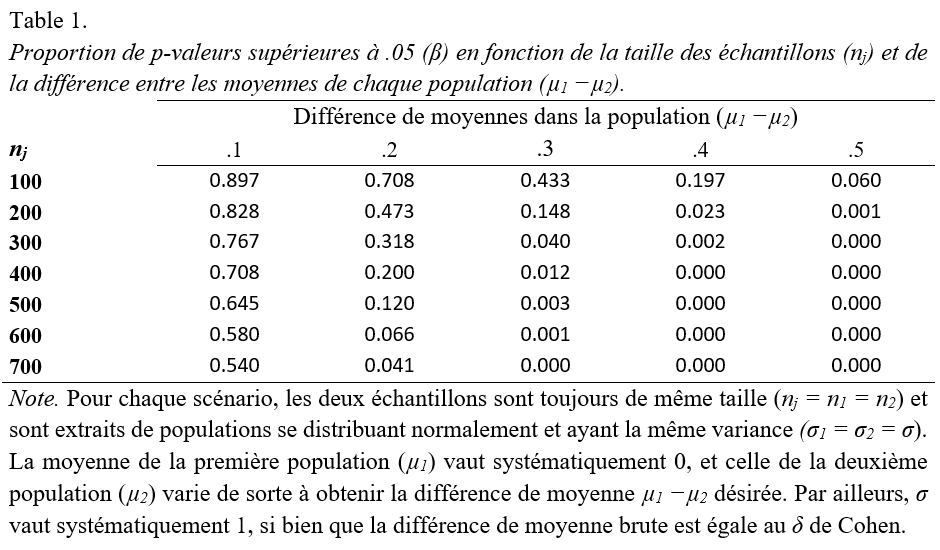
\includegraphics[width=0.95\linewidth]{C:/Users/Admin/Documents/Github projects/thesis/Chapitre 5/Illustration/Table1} \end{flushleft}
\newpage

Pour les scénarios de la première colonne, l'hypothèse nulle est vraie:
il n'y a pas de différence entre les moyennes de population. Puisque les
conditions d'application du test \(t\) de Student sont toutes
rencontrées, on est amené à rejeter l'hypothèse nulle, c'est-à-dire à
commettre une erreur de type I dans une proportion d'itération égale à
\(\alpha = 5\%\). Par conséquent, on est amené à \emph{ne pas} rejeter
l'hypothèse nulle \(95\%\) du temps (ce qui correspond à
\((1-\alpha)\%\))\endnote{Nous observons en réalité des proportions qui varient de $94.8\%$ à $95\%$, à cause du hasard d'échantillonnage, mais sur le long terme, lorsque le nombre d'itérations tend vers l'infini, toutes les proportions de non rejet de l'hypothèse nulle quand l'hypothèse nulle est vraie vont tendre vers $(1-\alpha) \%$.}.
Pour les scénarios envisagés dans toutes les autres colonnes de la Table
1, une vraie différence entre les moyennes de population existe, si bien
que le rejet de l'hypothèse nulle est la bonne décision. Pourtant, pour
plusieurs scénarios, le nombre d'itérations amenant à conclure au non
rejet de l'hypothèse nulle est bien supérieur au nombre d'itérations
amenant à conclure au rejet de l'hypothèse nulle, comme on peut le voir
à travers les valeurs \(\beta\). Par exemple, avec 100 sujets par
groupes et considérant \(\sigma_1=\sigma_2=1\), on ne détectera pas une
différence de moyenne de .1 dans près de 90\% des cas. Avec 700 sujets
par groupe, cette différence ne sera toujours pas détectée plus d'une
fois sur deux (\(\approx 54 \%\) des itérations). En présence d'un effet
non nul, cela se justifie par un manque de puissance des tests réalisés,
ce qui démontre bien qu'un non rejet de l'hypothèse nulle peut en fait
signifier deux choses: soit qu'il n'y a vraiment pas de différence entre
les moyennes des populations (ou autrement dit, que les différences
observées sont dûes au hasard), soit que le test n'est pas suffisamment
puissant pour détecter la différence. Or, le manque de puissance des
tests est récurrent dans la littérature, comme tendent à le montrer
diverses méta-analyses (Bakker, Van Dijk, \& Wicherts, 2012~; Button et
al., 2013~; Funder et al., 2014).

Pour éviter d'interpréter un test peu puissant comme un soutien en
faveur de l'hypothèse nulle, l'approche de la puissance est devenue
l'approche par défaut dans les années 80 pour tester l'équivalence
(Meyners, 2012). A travers cette approche qui est restée très populaire
(Quertemont, 2011), dans un premier temps, on définit ce qu'on considère
comme étant la plus petite valeur d'intérêt (en anglais, le ``SESOI''
pour ``Smaller Effect Size of Interest''), c'est-à-dire la taille
d'effet minimale requise pour considérer qu'un effet est pertinent.
Ensuite, on estime la puissance de notre test à détecter un effet de
cette
taille\endnote{On parle d'estimation et non de mesure, car la puissance du test dépend de $\sigma$, l'écart-type de la population, qu'on ne connait pas et devra donc estimer sur base de $S$, l'écart-type de l'échantillon (Schuirmann,1987).},
et si cette estimation atteind une valeur jugée satisfaisante (en
général, 80\%), alors on considère que l'on peut interpréter le non
rejet de l'hypothèse nulle d'absence d'effet comme soutien en faveur de
l'équivalence (Meyners, 2012~; Quertemont, 2011~; Schuirmann, 1987).
L'idée sous-jacente est que si l'effet est au moins aussi grand que les
bornes de la zone d'équivalence, sur le long terme, on devrait le plus
souvent rejeter l'hypothèse nulle. Par conséquent, un non rejet de
l'hypothèse nulle devrait généralement signifier que l'effet n'atteint
pas le SESOI et donc, que l'effet observé n'est pas pertinent. Bien que
ce raisonnement puisse sembler tentant, de prime abord, il présente
d'importantes limites.

Premièrement, le test n'a pas de bonnes propriétés asymptotiques. Ceci
est illustré au sein de la Table 2, dans laquelle nous envisageons les
mêmes scénarios que dans la Table 1 et ajoutons une contrainte de
puissance: nous décidons qu'on ne peut conclure à l'équivalence que si
l'on atteind une puissance de 80\% pour détecter une différence de
moyenne de .3. On constate qu'avec 100 sujets par groupes, aucune
itération n'amènera à conclure à l'équivalence, pas même lorsque la
différence entre les moyennes de population vaut 0. Cela s'explique par
le fait que l'on n'atteind jamais la puissance minimale de
\(80\%\).\endnote{Avec 100 sujets par groupe, on estime la puissance du test à $80\%$ lorsque l'estimation $d$ de Cohen vaut .3981. Par conséquent, un test sera susceptible de conclure à l'équivalence si les bornes de la zone d'équivalence, exprimée en mesure standardisée $d$ de Cohen, sont supérieures ou égales à .3981. Lorsqu'on fixe les bornes aux différences de moyennes $\pm .3$, cela n'est possible que si $S$ est inférieur ou égal à .7535. En effet, $d=\frac{\theta}{S} \leftrightarrow .3981 = \frac{.3}{S} \leftrightarrow S = \frac{.3}{.3981}=.7535$.  Or, avec 100 sujets par groupe, aucune estimation $S$ ne sera inférieure ou égale à .7535 lorsque $\sigma$ vaut 1.}
Par contre, une fois les échantillons assez grands pour s'assurer une
puissance de \(80\%\) pour détecter une différence de moyennes de
population de .3, lorsque la différence entre les moyennes de
populations est non nulle, la proportion d'itérations qui amènent à
conclure à l'équivalence diminue à mesure que la taille des échantillons
augmente. Par exemple, lorsque la différence de moyennes vaut .1 au
niveau des populations, on conclura à l'équivalence dans \(81\%\) des
itérations avec 200 sujets par groupe, contre seulement \(54\%\) des
itérations avec 700 sujets par groupe
\endnote{En comparant les Tables 1 et 2, on constate qu'avec 200 sujets par groupes, les proportions d'itérations de chaque scénario qui amènent à conclure à l'équivalence, dans la Table 2, sont inférieures aux proportions d'itérations de chaque scénarios qui amènent à ne pas rejeter l'hypothèse nulle, dans la Table 1. Plus les échantillons sont grands, moins on observera d'écart entre les 2 tables car la proportion d'itérations qui ne pourront amener à conclure à l'équivalence en raison d'un manque de puissance diminuera. En effet, plus la taille des échantillons sera grande, plus la valeur maximale de $S$ permettant d'assurer la puissance des $80\%$ sera élevée. Par exemple, avec 200 sujets par groupes, la valeur maximale autorisée pour $S$ sera de $\frac{.3}{.2808}=1.07$. Avec 300 sujets par groupes, la valeur maximale autorisée pour $S$ sera de $\frac{.3}{.2291}=1.31$. Par conséquent, plus les tailles d'échantillons seront grandes, moins il sera probable que $S$ dépasse le seuil autorisé.}.

\begin{flushleft}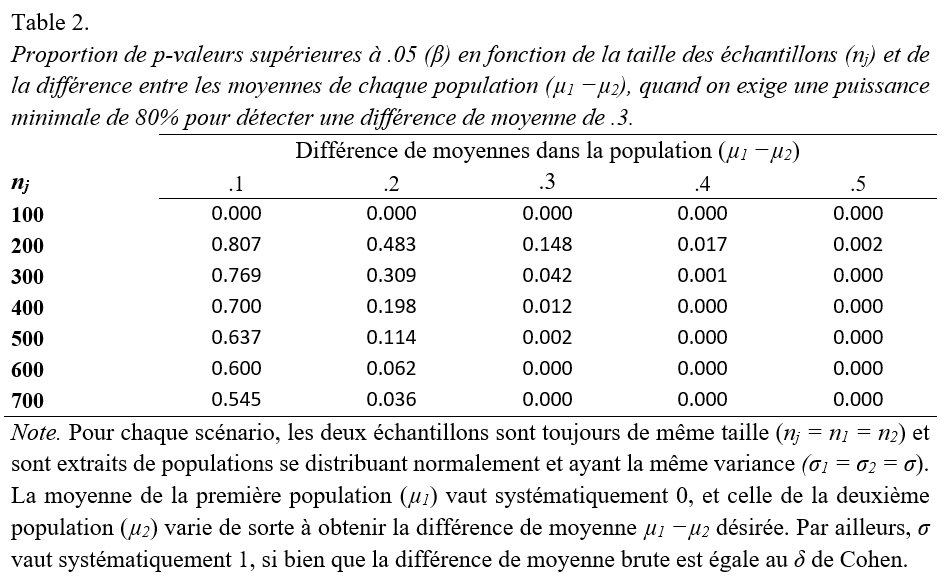
\includegraphics[width=0.95\linewidth]{C:/Users/Admin/Documents/Github projects/thesis/Chapitre 5/Illustration/Table2} \end{flushleft}

Deuxièmement, pour une taille d'échantillon donnée, plus l'erreur (la
variabilité des scores au sein de chaque groupe) sera grande (Meyners,
2012~; Schuirmann, 1987), plus la probabilité de conclure à
l'équivalence augmentera. Ce dernier point est illustré au sein de la
Figure \ref{fig:schuirman2}, dans le contexte de la comparaison de deux
moyennes. Sur l'axe des abscisses, on représente différentes estimations
de la différence de moyenne (\(\bar{X_1}-\bar{X_2}\)) et sur l'axe des
ordonnées, la précision des estimations \(\bar{X_1}-\bar{X_2}\)
(\(S\sqrt{\frac{2}{n}}\) correspond à l'estimation de l'erreur standard
de \(\bar{X_1}-\bar{X_2}\), avec \(S\) étant l'écart-type poolé et \(n\)
la taille de chaque échantillon, lorsque les échantillons ont tous les
deux la même taille et sont extraits de population ayant la même
variance)\endnote{Par facilité, à l'instar de Schuirman (1987), on envisage le cas où les échantillons sont de même taille et que l'on suppose que la condition d'homogénéité des variances est respectée. Notons cependant que d'après Schuirman, ce raisonnement peut être généralisé aux scénarios où les deux échantillons n'ont pas la même taille et sont extraits de population n'ayant pas la même variance.}.
Le triangle grisé représente l'ensemble des combinaisons
estimation/précision qui vont amener à conclure à l'équivalence, avec
l'approche de la puissance, lorsqu'on travaille avec des échantillons de
taille 50, en acceptant un risque \(\alpha\) de 5\% et en exigeant une
puissance minimale de 80\% pour détecter une différence de 20 unités
(\(|\theta_j=20|,\;j=1,2\)). Dans cet exemple, pour toutes les valeurs
de \(S\sqrt{\frac{2}{n}}\) supérieures à 7.07 aucune estimation de
différence de moyennes ne permettra de conclure à l'équivalence (pas
même 0) puisque la puissance du test à détecter une différence de 20
unités est inférieure à 80\%. Pour toutes les valeurs de
\(S\sqrt{\frac{2}{n}}\) inférieures à 7.07, on constate que plus notre
estimation de \(\bar{X_1}-\bar{X_2}\) est précise (lorsqu'on se déplace
du haut vers le bas, sur l'axe des ordonnées), plus l'estimation doit
être proche de 0 pour pouvoir conclure à l'équivalence. Comme on peut le
voir à travers le triangle hachuré sur la Figure 1, cette propriété peu
désirable n'est pas partagée par le TOST, un test d'équivalence que nous
allons décrire ci-dessous (Schuirmann, 1987).

\begin{figure}

{\centering 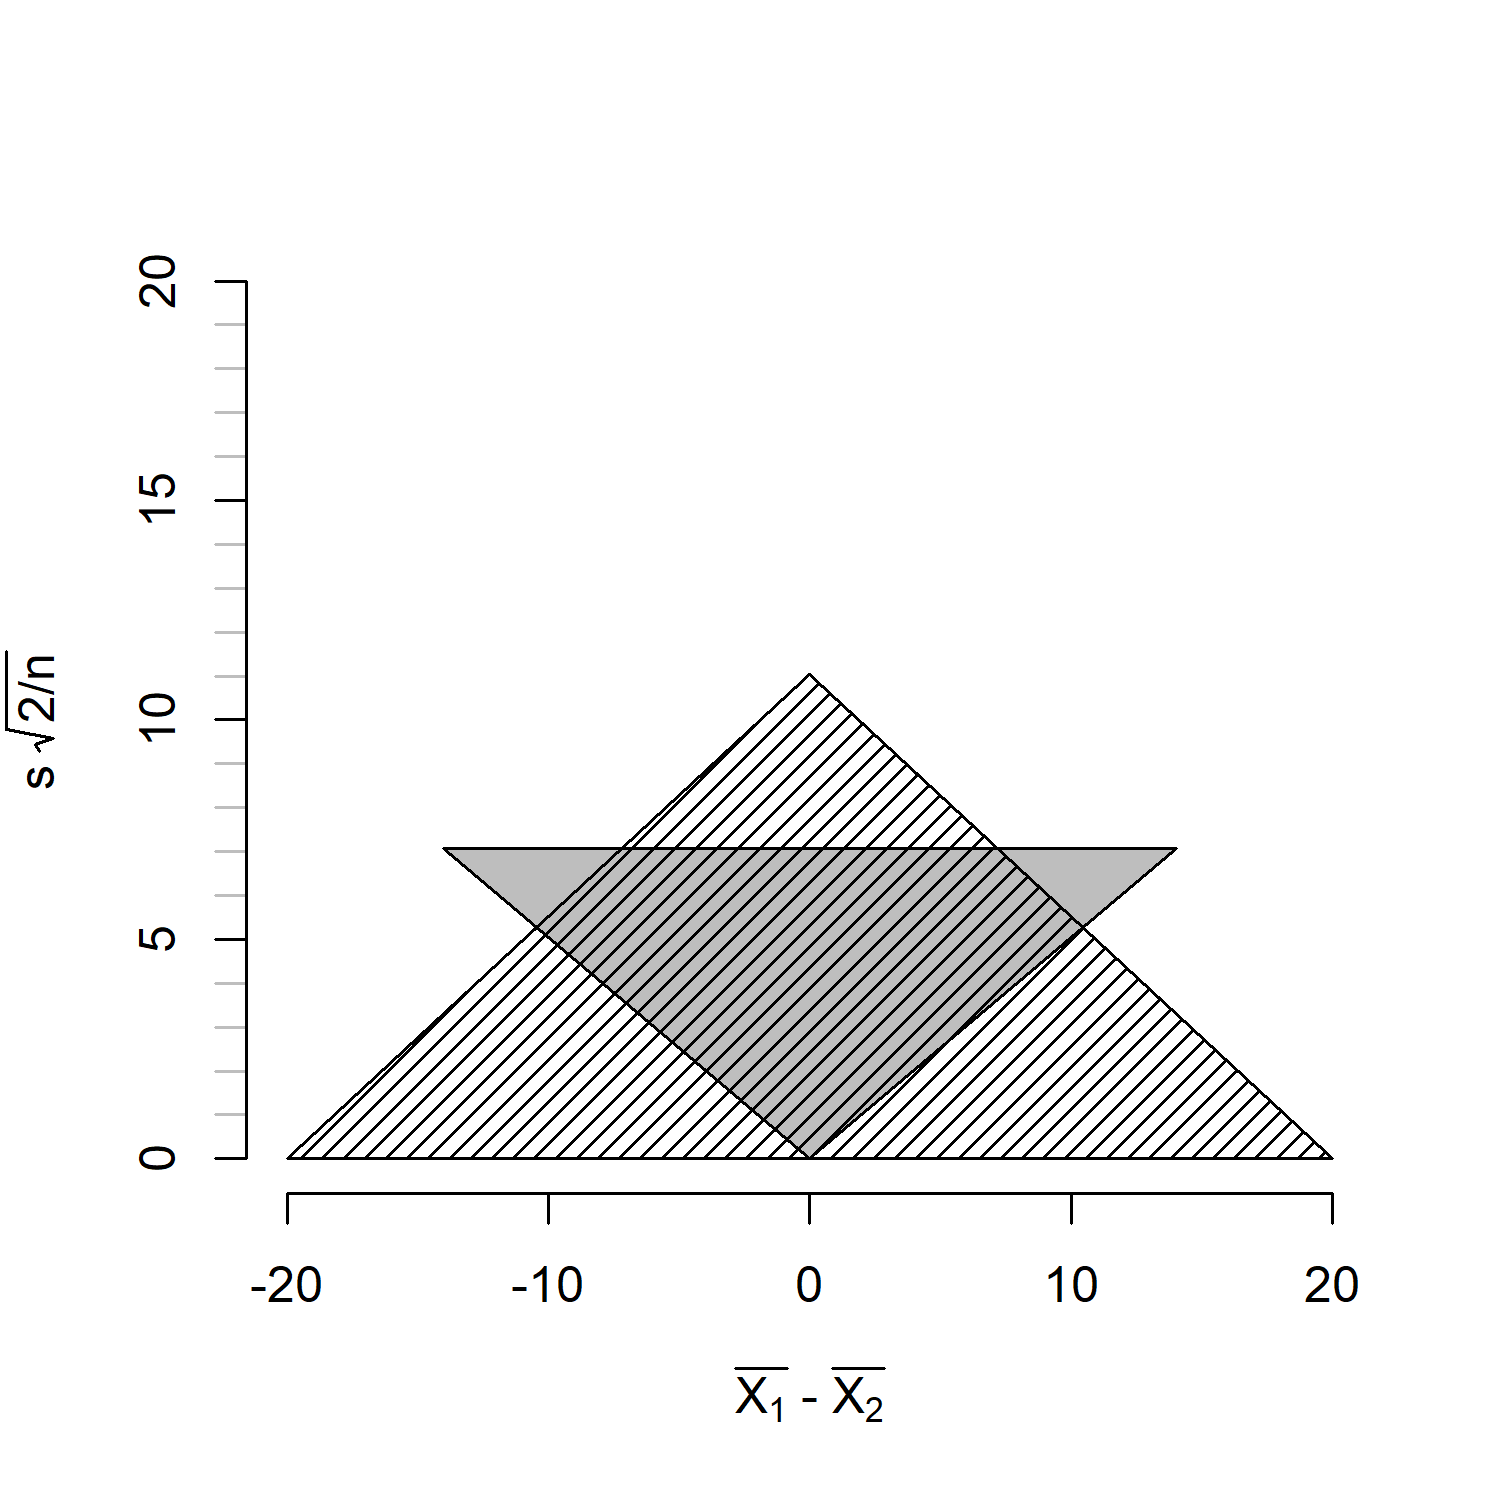
\includegraphics[width=0.4\linewidth]{C:/Users/Admin/Documents/Github projects/thesis/Chapitre 5/Illustration/Fig1} 

}

\caption{Région d'équivalence pour l'approche de la puissance (zone grisée) et pour le TOST (zone hachurée), pour l'exemple où $|\theta$|=20, n = 50 et $\alpha=.05$}\label{fig:schuirman2}
\end{figure}

\newpage

\hypertarget{les-tests-duxe9quivalence}{%
\subsection{Les tests d'équivalence}\label{les-tests-duxe9quivalence}}

Avec les tests d'équivalence, il n'est pas possible de démontrer qu'un
effet vaille exactement zéro (Meyners, 2012). Il est par contre possible
de montrer que l'effet observé est suffisamment petit pour être jugé non
pertinent. Or, cela peut s'avérer précieux dans de nombreuses
situations, par exemple pour justifier la décision de regrouper
plusieurs groupes de sujets ensemble (Rogers, Howard, \& Vessey, 1993),
pour contrôler qu'il n'y ait pas de différence trop importante entre les
groupes sur base de critères autres que le (ou les) facteur(s)
d'intérêts en cas de quasi-expérience (Seaman \& Serlin, 1998) ou encore
pour falsifier une théorie qui prônerait en faveur d'un effet dépassant
une certaine taille (Anderson \& Maxwell, 2016~; Lakens, 2017).

Le point de départ des tests d'équivalence est de définir \(\theta_1\)
et \(\theta_2\), les bornes inférieures et supérieures de la zone
d'équivalence, cette dernière contenant l'ensemble des valeurs jugées
trop petites pour être susceptibles de nous intéresser. Ces bornes
peuvent être exprimées soit dans l'unité des données brutes, soit en
terme standardisé, mais doivent être définies avant la récolte des
données (Anderson \& Maxwell, 2016~; Lakens, Scheel, \& Isager, 2018).
Il existe ensuite plusieurs approches pour démontrer que l'effet observé
se situe dans la zone d'équivalence (voir Meyners, 2012, par exemple).
Parmis celles-ci, une approche très simple est celle du ``Two one-sided
tests'' (Lakens, 2017~; Schuirmann, 1987), plus communément appelé le
TOST
\endnote{Il existe des alternatives au TOST qui sont très légèrement plus puissantes, mais le gain marginal en termes de puissance est contrebalancé par un niveau de complexité beaucoup plus élevé (Meyners, 2012).}.
Le principe est de définir deux hypothèses nulles. La première est que
l'effet observé est inférieur à la borne inférieure de la zone
d'équivalence:
\[\it H0_1: \theta < \theta_1, \; avec \; \theta_1 \neq 0\] La deuxième
est que l'effet observé est supérieur à la borne supérieure de la zone
d'équivalence:
\[\it H0_2: \theta > \theta_2, \; avec \; \theta_2 \neq 0\] Lorsque les
deux hypothèses nulle peuvent être simultanément rejetées, on peut
conclure à l'équivalence (Seaman \& Serlin, 1998). Cela équivaut,
statistiquement parlant, à montrer que l'intervalle de confiance à
\((1-2\times\alpha)\%\) est entièrement inclus dans la zone
d'équivalence (Lakens, 2017~; Seaman \& Serlin, 1998). Notons qu'il
n'est pas nécessaire de reporter les résulats des deux tests
unilatéraux, lorsqu'on réalise le TOST: il suffit de reporter les
résultats du test associé à la plus petite valeur de statistique (et par
conséquent, à la plus grande \(p\)-valeur). En effet, si ce test amène à
conclure au rejet de l'hypothèse nulle, le second test amènera
automatiquement à la même conclusion (Lakens, Scheel, \& Isager, 2018~;
Rogers, Howard, \& Vessey, 1993). Cette remarque reste vraie dans le cas
particulier où les deux tests sont associés à la même valeur de
statistique puisque dans ce cas, les deux tests mèneront à une
conclusion identique (Rogers, Howard, \& Vessey, 1993). Notons également
qu'il n'est pas nécessaire de procéder à une correction du risque alpha
dûe à la réalisation simultanée de deux tests. En effet, une erreur de
type I (rejeter à tort l'hypothèse nulle) ne peut être commise que si
l'hypothèse nulle est vraie. Or, les deux hypothèses nulles testées sont
mutuellement exclusives: il n'est pas possible que \(\theta\) soit
simultanément inférieur à \(\theta_1\) (ce qui correspond à
\(\it H0_1\)) et supérieur à \(\theta_2\) (ce qui correspond à
\(\it H0_2\)).

Jusqu'il y a peu, le TOST n'était pas disponible dans la plupart des
logiciels, à l'exception de Minitab, ce qui constituait un frein
important à son usage. Pour cette raison, Lakens (2016) a créé le
package R ``TOSTER'' et plus récemment encore, ce même package a été
implémenté dans Jamovi
\endnote{Jamovi est un logiciel clic-bouton entièrement gratuit qui gagne en popularité et qui présente, parmi ses nombreux avantages, le fait d'être particulièrement convivial. Dans la mesure où la plupart des chercheurs sont plus enclins à utiliser des procédures si elles sont implémentées dans ce type de logiciel (Fraas $\&$ Newman, 2000), cela constitue une excellente nouvelle pour le devenir du TOST dans la recherche en psychologie.}.
Tant dans R que dans Jamovi, le package compare simultanément l'effet
observé à l'absence d'effet (cela correspond au test traditionnel) ainsi
qu'aux deux bornes de la zone d'équivalence (cela correspond au TOST).
Il en découle 4 conclusions distinctes possibles (Lakens, 2017), qui
sont illustrées dans la figure \ref{fig:equiv1} dans le contexte de la
comparaison de deux moyennes indépendantes:

\begin{figure}

{\centering 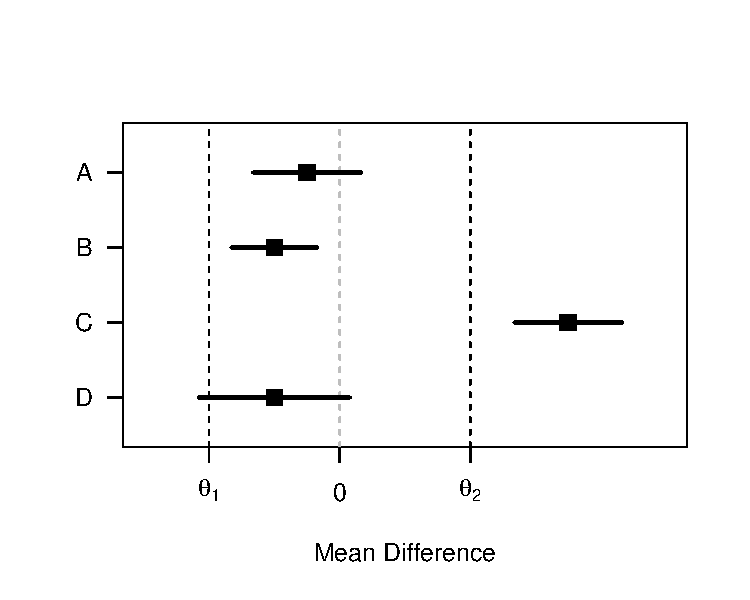
\includegraphics[width=0.8\linewidth]{template_files/figure-latex/equiv1-1} 

}

\caption{Différence de moyennes ($\bar{X_1}-\bar{X_2}$) et IC à $1-2\alpha\%$ autour de la différence de moyennes ($\bar{X_1}-\bar{X_2}$) pour 4 scénarios distincts.}\label{fig:equiv1}
\end{figure}

\begin{enumerate}
\def\labelenumi{(\arabic{enumi})}
\item
  La différence de moyenne observée diffère significativement des deux
  bornes d'équivalence, mais pas de 0 (scénario A, Figure
  \ref{fig:equiv1}): dans ce cas, on conclura à l'absence d'un effet au
  moins aussi grand que les bornes d'équivalence.
\item
  La différence de moyenne observée diffère significativement des deux
  bornes d'équivalence ainsi que de 0 (scénario B, Figure
  \ref{fig:equiv1}): on conclura alors qu'il existe un effet non nul,
  mais qui ne dépasse pas une certaine taille fixée par les bornes.
  C'est ce qui arrive typiquement lorsqu'on travaille avec de très
  grands échantillons, si bien que le test traditionnel est très
  puissant, même pour détecter des effets très petits (Rogers, Howard,
  \& Vessey, 1993).
\item
  La différence de moyenne observée diffère significativement de 0, mais
  ne diffère pas significativement d'au moins une des deux bornes
  d'équivalence (scénario C, Figure \ref{fig:equiv1}): on conclura alors
  à la présence d'un effet non nul (Rogers, Howard, \& Vessey, 1993).
\item
  La différence de moyenne observée ne diffère significativement ni d'au
  moins une des deux bornes d'équivalence, ni de 0 (scénario D, Figure
  \ref{fig:equiv1}): c'est ce qui arrive lorsque les données sont si
  imprécises qu'on ne peut tirer aucune conclusion. Les données semblent
  compatibles tant avec un effet nul qu'avec un effet supérieur au
  SESOI.
\end{enumerate}

\hypertarget{duxe9finir-les-bornes-de-la-zone-duxe9quivalence}{%
\subsection{Définir les bornes de la zone
d'équivalence}\label{duxe9finir-les-bornes-de-la-zone-duxe9quivalence}}

L'aspect le plus compliqué dans la réalisation du TOST est la définition
des bornes d'équivalence. Dans certains cas, il est possible de définir
un critère objectif qui permettra de déterminer à partir de quand un
effet est jugé pertinent (Lakens, Scheel, \& Isager, 2018). Dans ce cas,
établir l'équivalence revient à rejeter la présence d'un effet ayant un
quelconque intérêt pratique (Rogers, Howard, \& Vessey, 1993). Par
exemple, Burriss et al. (2015) avaient émis l'hypothèse qu'une
augmentation de la rougeur de la peau chez femmes les rendraient plus
attractives pour les hommes en période d'ovulation. Or, une telle
hypothèse n'est crédible que si le changement facial est visible à
l'oeil nu. Dans ce contexte, le SESOI serait la plus petite variation
dans la rougeur de la peau qu'il est possible de détecter à l'oeil nu
(Lakens, Scheel, \& Isager, 2018). Il est également parfois possible
pour des experts de déterminer expérimentalement ce qui constitue un
changement important, pour certaines échelles fréquemment utilisées en
vue mesurer des construits psychologiques. Button et al. (2015), par
exemple, ont interrogé un grand nombre de patients dépressifs quant à
leur ressenti subjectif en termes d'amélioration de leur dépression au
cours d'un certain laps de temps, et ont comparé leur réponses à la
différence de scores obtenus à l'aide du BDI
\endnote{Le BDI (Beck Depression Inventory) est une échelle auto-rapportée évaluant les symptômes cognitifs courants de la dépression.  Cette échelle est constituée de 21 items évalués à l'aide des échelles de Likert allant de 0 à 3, ce qui donne un score total compris entre 0 et 63 qui sera d'autant plus élevé que la dépression sera sévère (Button et al., 2015).}
dans ce même laps de temps (Lakens, Scheel, \& Isager, 2018). Cela leur
a permis de déterminer ce qu'il considérait comme étant une différence
pratiquement significative sur l'échelle du BDI. Malheureusement, il
n'est pas toujours possible d'établir un critère objectif en vue de
définir les bornes d'équivalence. Dans ce cas, il existe diverses
stratégies, plus subjectives, en vue d'établir ces bornes. En les
utilisant, il faut cependant avoir conscience du fait que la question à
laquelle nous répondons varie en fonction de la stratégie utilisée.

Il est possible de déterminer des bornes en s'inspirant de balises
existantes, en vue d'exclure la présence d'un effet jugé petit, moyen ou
grand par ces balises (Lakens, Scheel, \& Isager, 2018). Notons que si
cette stratégie est tentante de par sa simplicité, elle doit être
utilisée avec prudence. D'abord, un effet ne devrait être qualifié de
petit, moyen ou grand qu'en comparaison à d'autres effets connus, et non
sur base d'impressions qualitatives (Gignac \& Szodorai, 2016). Dit
autrement, il est important d'avoir un cadre de référence pour juger de
la taille d'un effet. Or, les balises de Cohen (en l'occurence, les
balises les plus célèbres et les plus largement utilisées) sont
dépourvues de ce cadre de référence, puisqu'elles ont été établies à une
époque où très peu de chercheurs se préoccupaient de la taille des
effets étudiés (Funder \& Ozer, 2019). Depuis Cohen, certains chercheurs
ont déployé de gros efforts en vue d'établir de nouvelles normes sur
base d'analyses systématiques quantitative de la litérature. Gignac \&
Szodorai (2016), par exemple, ont établi de nouvelles balises pour
interpréter le \(r\) de Pearson, en définissant les quartiles d'une
distribution de 708 mesures dérivées de méta-analyses issues de la
psychologie sociale et de la personnalité. C'est de la sorte qu'ils ont
proposé d'interpréter respectivement des mesures de 0.10, 0.20 et 0.30,
dans ces domaines de la psychologie, comme représentant des effets
relativement petits, typiques et relativement larges. Ces normes ont
également été approuvées par Funder \& Ozer (2019)
\endnote{Funder $\&$ Ozer (2019) ont relevé plusieurs enquêtes ayant calculé un $r$ de Pearson moyen de .21 sur base d'effets publiés dans la litérature en psychologie sociale et en psychologie de la personnalité. Par ailleurs, ils rappellent qu'en raison du biais de publication, un chercheur obtenant un $r$ de Pearson de .21 dans une nouvelle étude peut être assuré d'avoir détecté un effet plus grand que généralement trouvé}.
Ensuite, les balises ne prennent pas en compte le contexte de l'étude si
bien que statuer sur la taille d'un effet ne fournit pas nécessairement
d'information sur sa valeur. Imaginons un antidépresseur B qui permette
de réduire très légèrement les symptômes de dépression par rapport à un
antidépresseur A déjà présent sur le marché, et qui en outre coûte moins
cher. Même si statistiquement parlant, on observe une très faible taille
d'effet, une analyse coût/bénéfice amènerait très vraisemblablement à
conclure à la pertinence de cet effet. Pour cela, les balises devraient
toujours être utilisées en dernier recours, lorsqu'on ne dispose
d'aucune autre information (Gignac \& Szodorai, 2016).

La taille des échantillons d'une étude est une information sur laquelle
nous pouvons également nous baser en vue de fixer des bornes
d'équivalence. Dans le contexte d'une réplication d'étude, cette
information peut servir à déterminer si la puissance de l'outil utilisé
par le chercheur d'origine était suffisante en vue de tester l'effet
ciblé. Une stratégie proposée par Lakens, Scheel, \& Isager (2018)
consiste à définir comme borne d'équivalence le plus petit effet que
l'étude d'origine aurait pu détecter comme étant
significative.\endnote{Dans le contexte d'une réplication, il nous semble souvent plus logique de réaliser le test d'équivalence en unilatéral, puisque l'étude d'origine précisera généralement le sens de l'effet observé. C'est pourquoi nous parlons ici de bornd d'équivalence au singulier}.
L'idée sous-jacente est la suivante: bien qu'idéalement, les chercheurs
devraient toujours spécifier ce qu'ils considèrent comme étant le plus
petit effet d'intérêt, cette pratique n'est pas encore commune.
Heureusement, même lorsqu'un auteur ne statue pas explicitement sur ce
qu'il considère comme étant un effet pertinent, la taille des
échantillons qu'il utilise aura un impact sur la taille des effets que
l'on sera capable de mettre en évidence (en effet, plus les échantillons
sont petits, plus l'effet observé doit être grand pour pouvoir être
détecté comme étant significatif). Imaginons par exemple qu'un auteur
compare les moyennes de deux groupes de 30 sujets à l'aide d'un test
\(t\) de Student (par facilité, considérons les conditions d'application
de ce test comme étant toutes respectées). Avec ces tailles
d'échantillon, on conclura au rejet de l'hypothèse nulle si la
statistique \(t\) de Student vaut au minimum 2.002. Compte tenu de la
relation directe entre la statistique \(t\) de Student et le \(d\) de
Cohen (voir chapitre 4), on en déduit qu'on conclura au rejet de
l'hypothèse nulle si le \(d\) de Cohen est supérieur ou égal à 0.517. Si
l'on fixe 0.517 comme borne d'équivalence, et que l'on démontre lors
d'une réplication que l'effet observé est significativement inférieur à
cette borne, on suspectera que l'étude d'origine n'aurait pu détecter
proprement l'effet qu'elle prétendait détecter. Une autre stratégie,
proposée par Simonsohn, Nelson, \& Simmons (2014) consiste à déterminer
la taille d'effet que l'étude d'origine aurait pu détecter avec une
puissance de \(33\%\), et à utiliser cette information pour définir la
borne d'équivalence. Par exemple, avec une hypothèse bilatérale, un test
\(t\) de Student aura une puissance de \(33\%\) pour détecter un effet
de taille 0.399 avec 30 sujets par groupe (à condition que les
conditions d'application du test soient toutes respectées). Si lors de
la réplication, on obtient un effet significativement inférieur à 0.399,
on en déduira que sur le long terme, la probabilité que l'outil
d'origine puisse proprement détecter un effet de cette taille était
inférieure à \(33\%\), ce qui remet sa pertinence en cause
\endnote{Bien entendu, la valeur $33\%$ a une dimension arbitraire, comme chaque fois que l'on fixe une valeur par défaut.}.

Hors du contexte des réplications d'études, on peut également se baser
sur la taille des échantillons que l'on est apte à collecter soi-même,
en vue de déterminer si l'on dispose d'assez de ressources pour détecter
un effet ciblé (Lakens, Scheel, \& Isager, 2018). Par exemple, si nous
sommes dans l'incapacité de collecter des échantillons de plus de 2000
personnes, il y a certains effets que nous ne pourrons jamais détecter
avec une puissance suffisante. Il est possible de déterminer la taille
d'effet que nous sommes certains de pouvoir détecter avec suffisamment
de puissance (ou autrement dit, dans un pourcentage raisonnable de cas,
sur le long terme). \emph{Si l'on utilise cette information pour fixer
la (ou les) borne(s) d'équivalence et que l'on conclut effectivement à
l'équivalence, la conclussion sera que pour détecter proprement l'effet
que nous ciblons, il est indispensable de collecter de plus grands
échantillons.}

\hypertarget{comparaison-du-tost-et-du-sgpv}{%
\subsection{Comparaison du TOST et du
SGPV}\label{comparaison-du-tost-et-du-sgpv}}

\begin{center}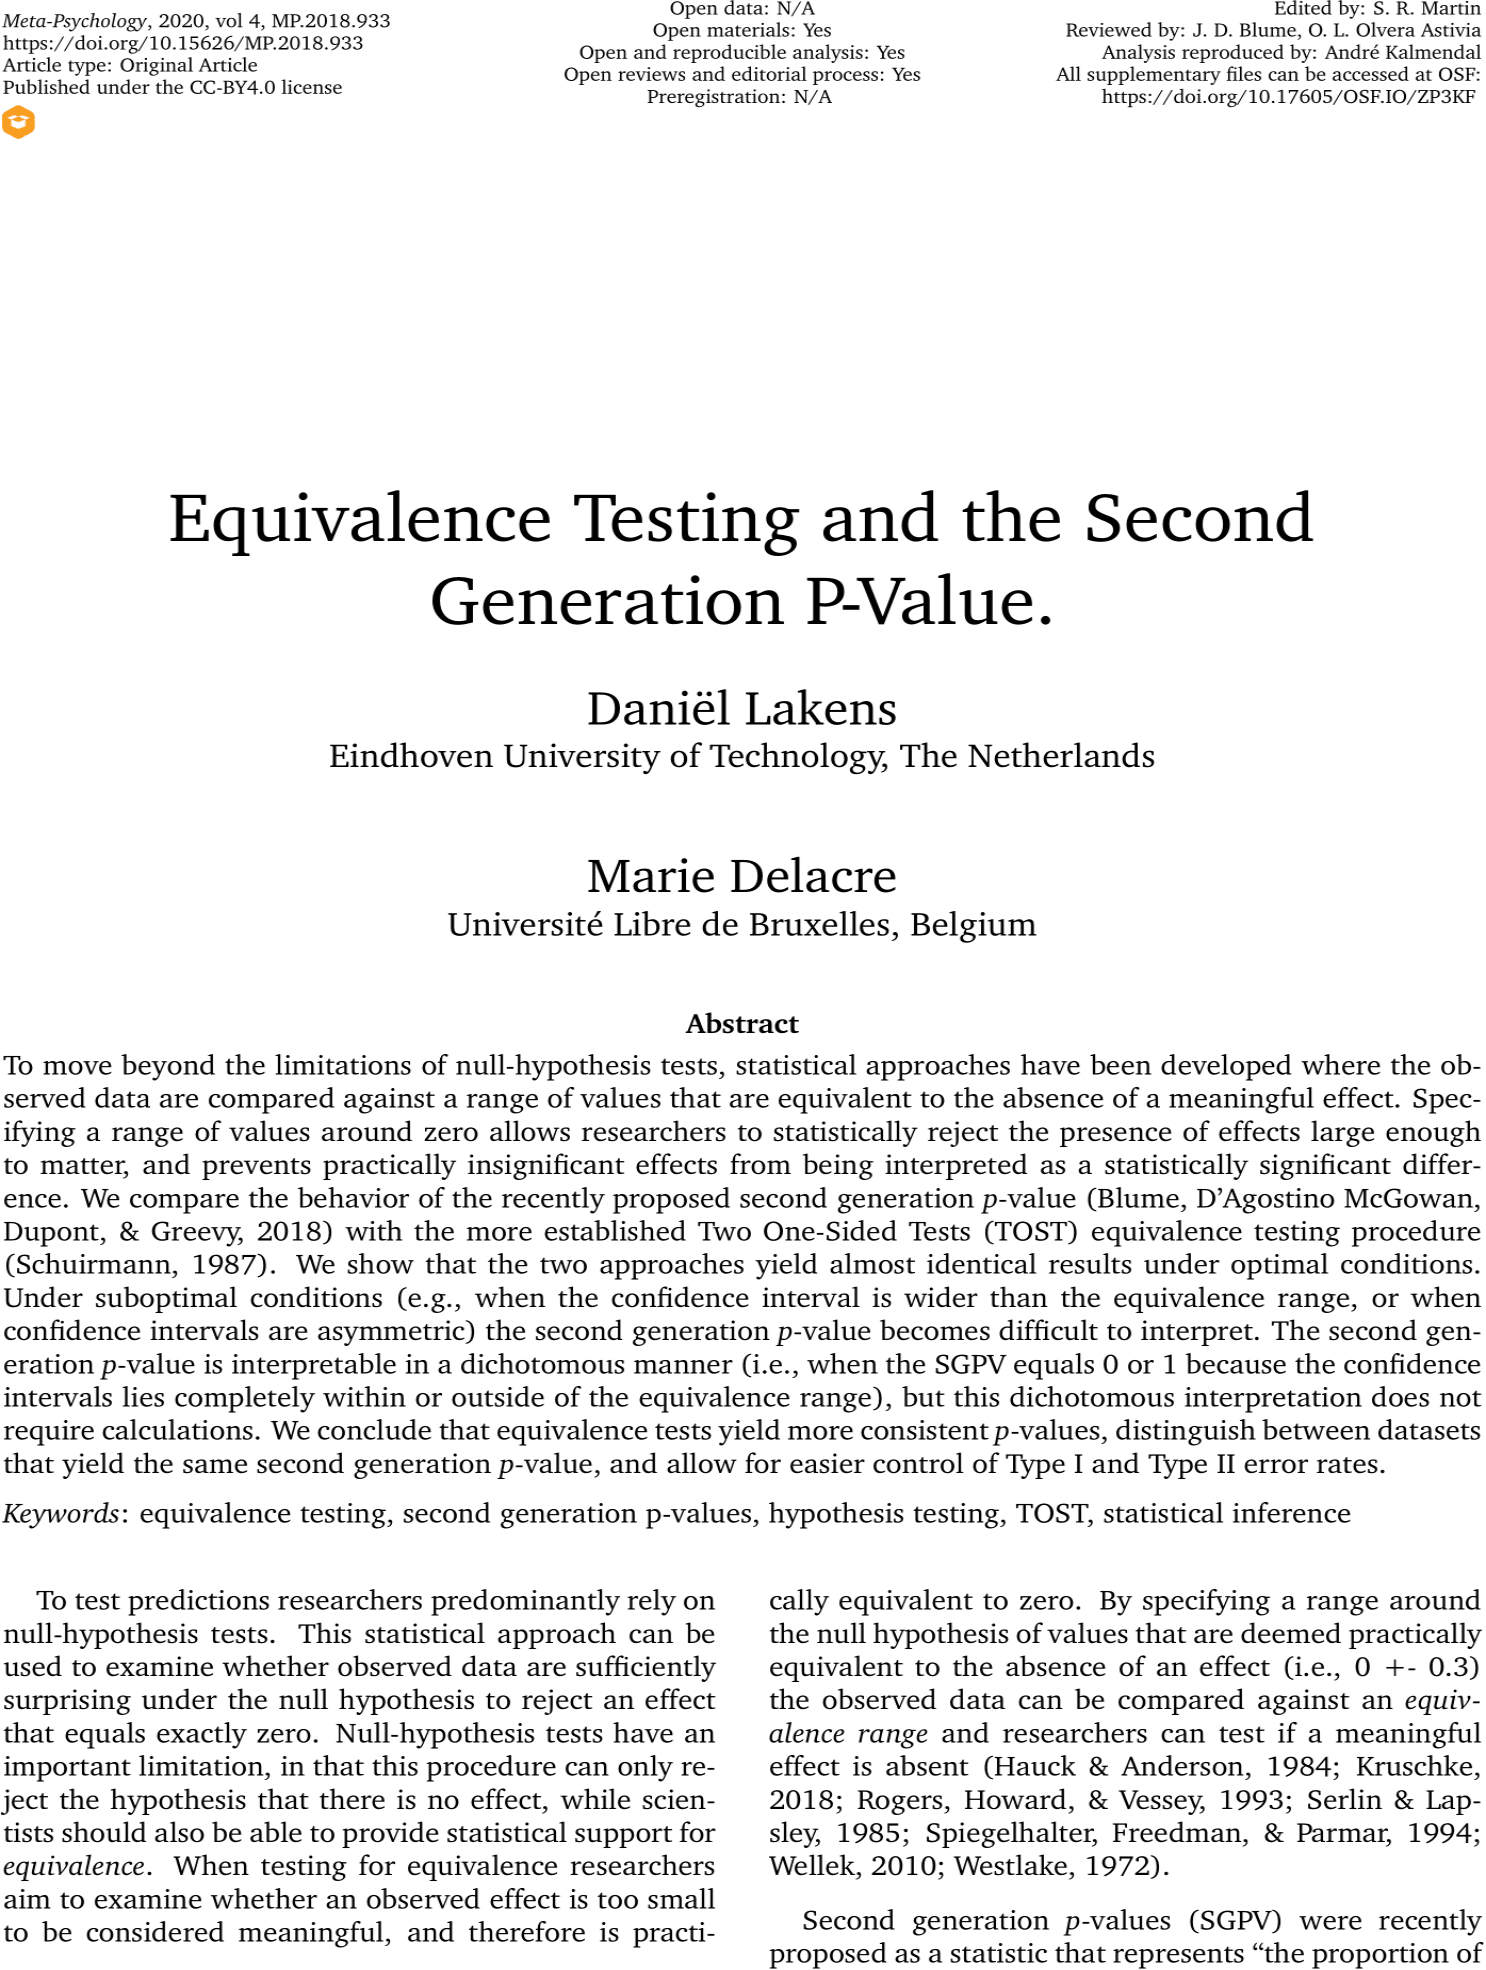
\includegraphics[width=0.92\linewidth]{C:/Users/Admin/Documents/Github projects/thesis/Chapitre 5/Chapitre 5-1} \end{center}

\begin{center}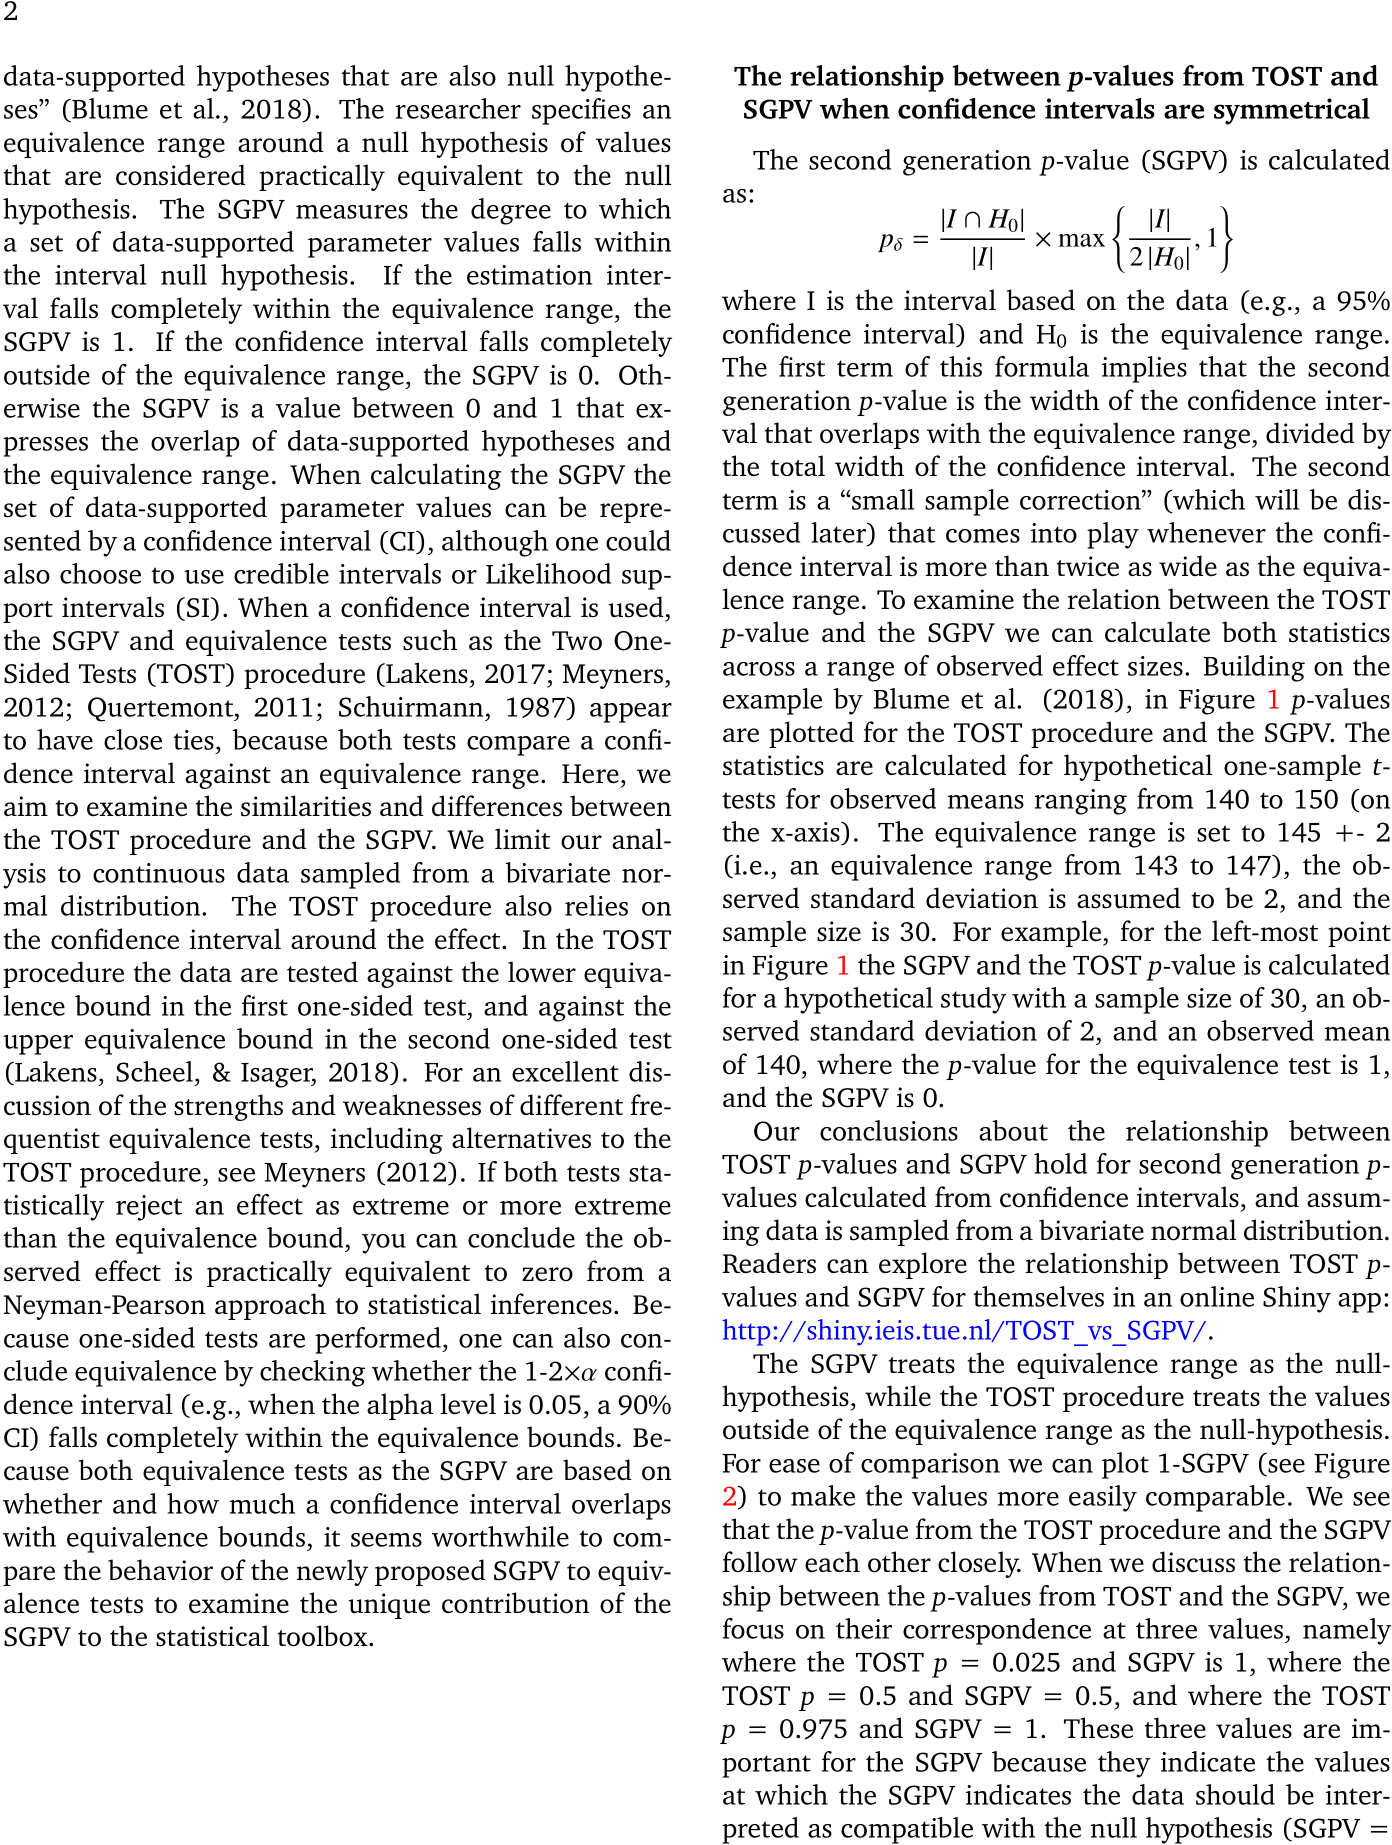
\includegraphics{C:/Users/Admin/Documents/Github projects/thesis/Chapitre 5/Chapitre 5-2} \end{center}

\begin{center}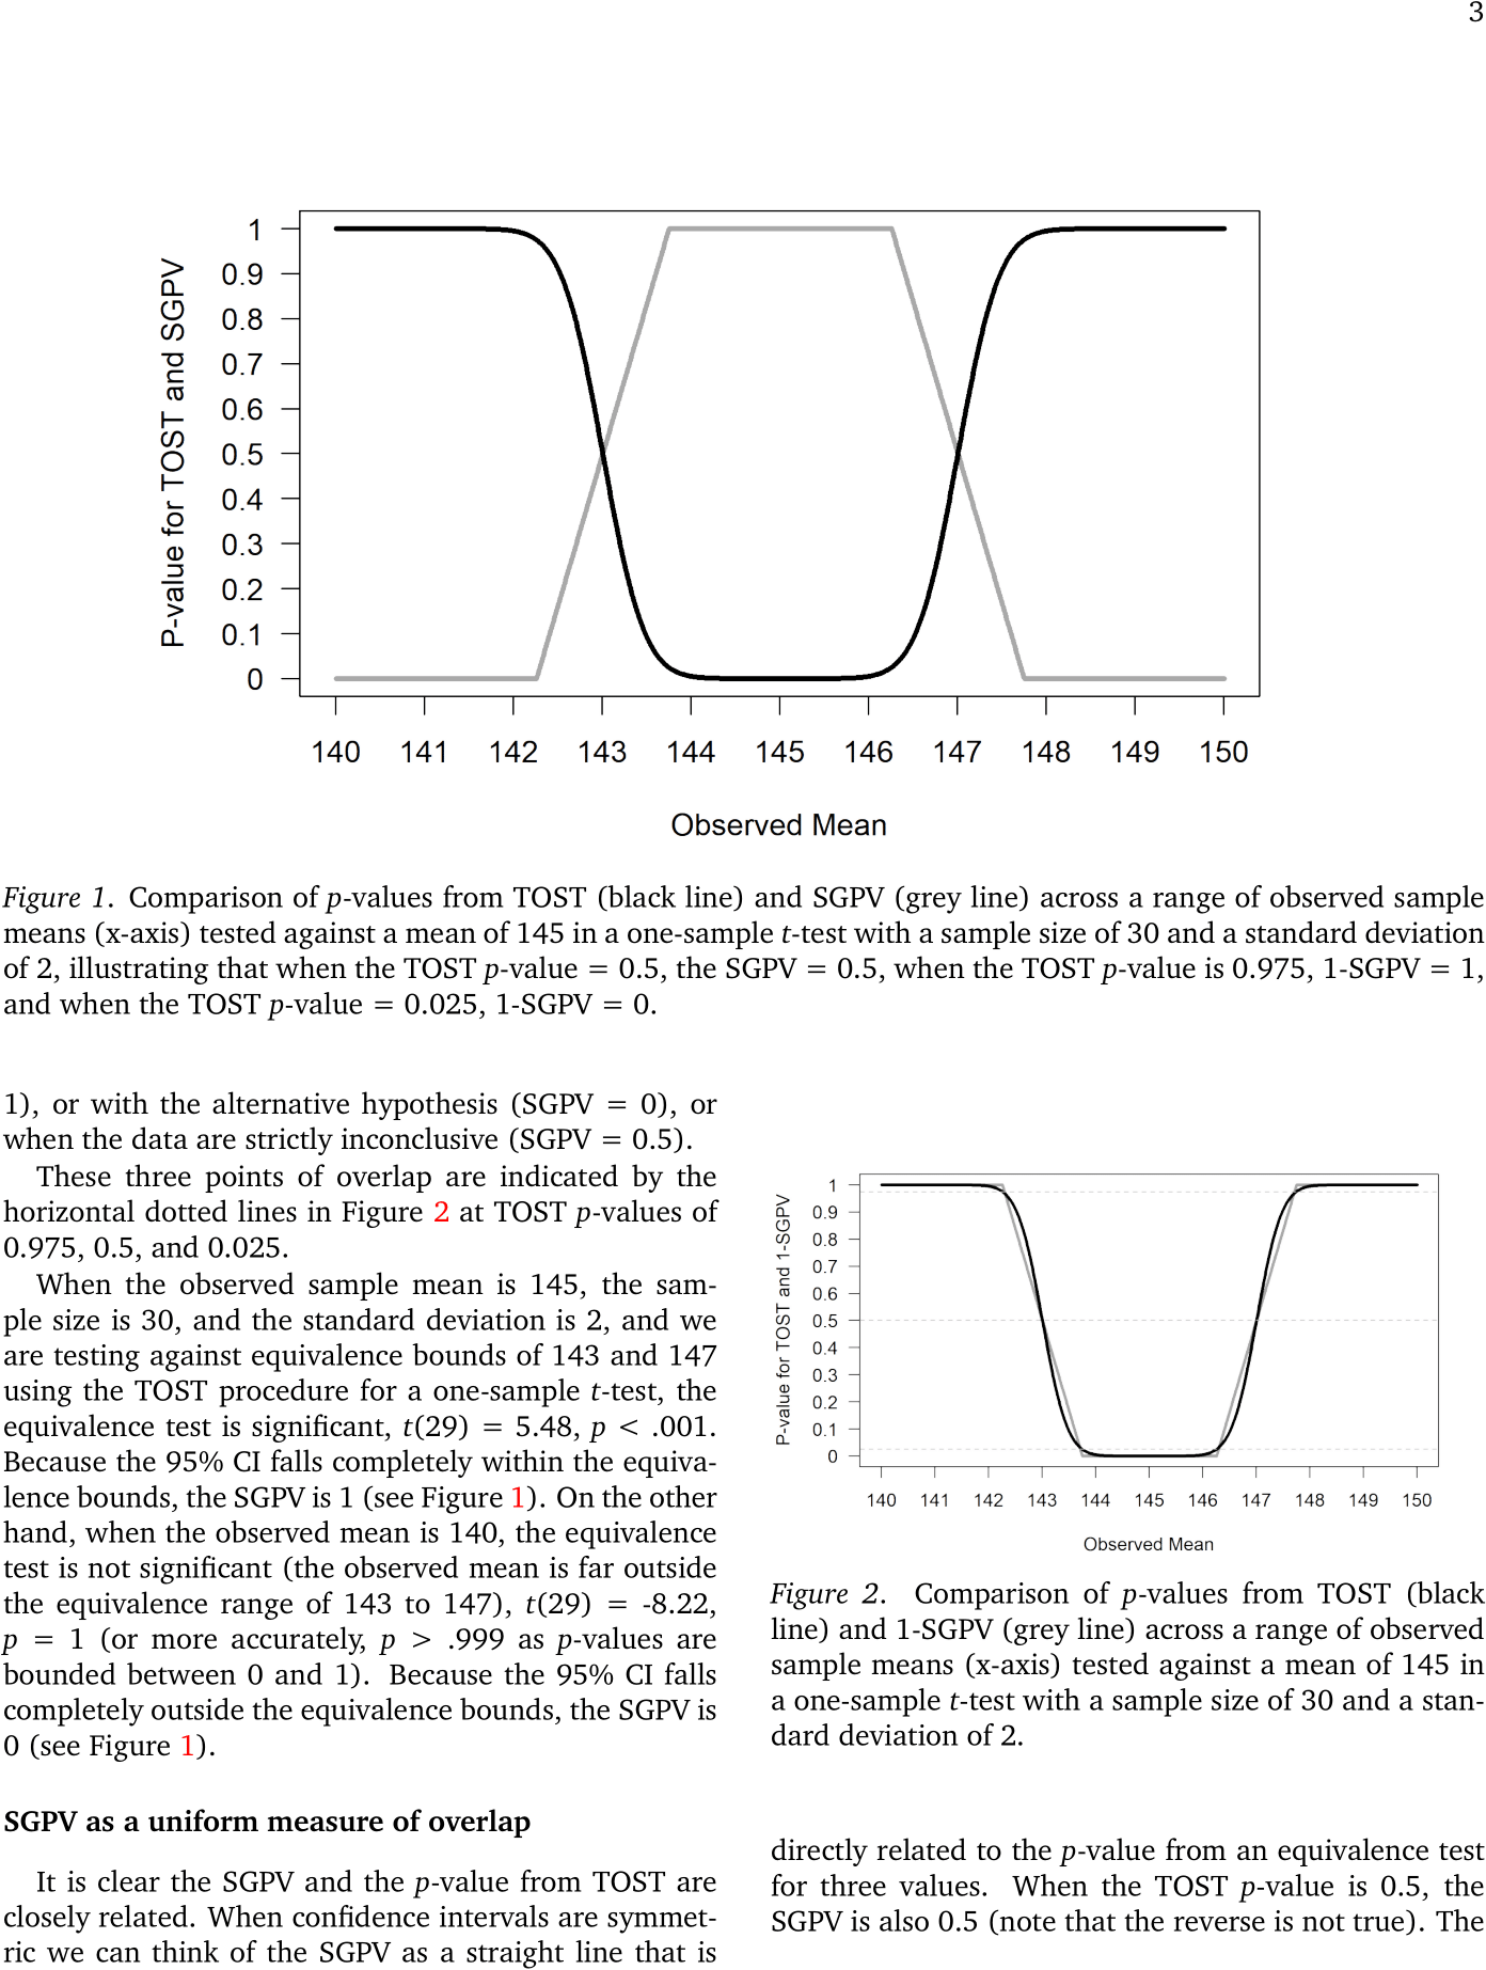
\includegraphics{C:/Users/Admin/Documents/Github projects/thesis/Chapitre 5/Chapitre 5-3} \end{center}

\begin{center}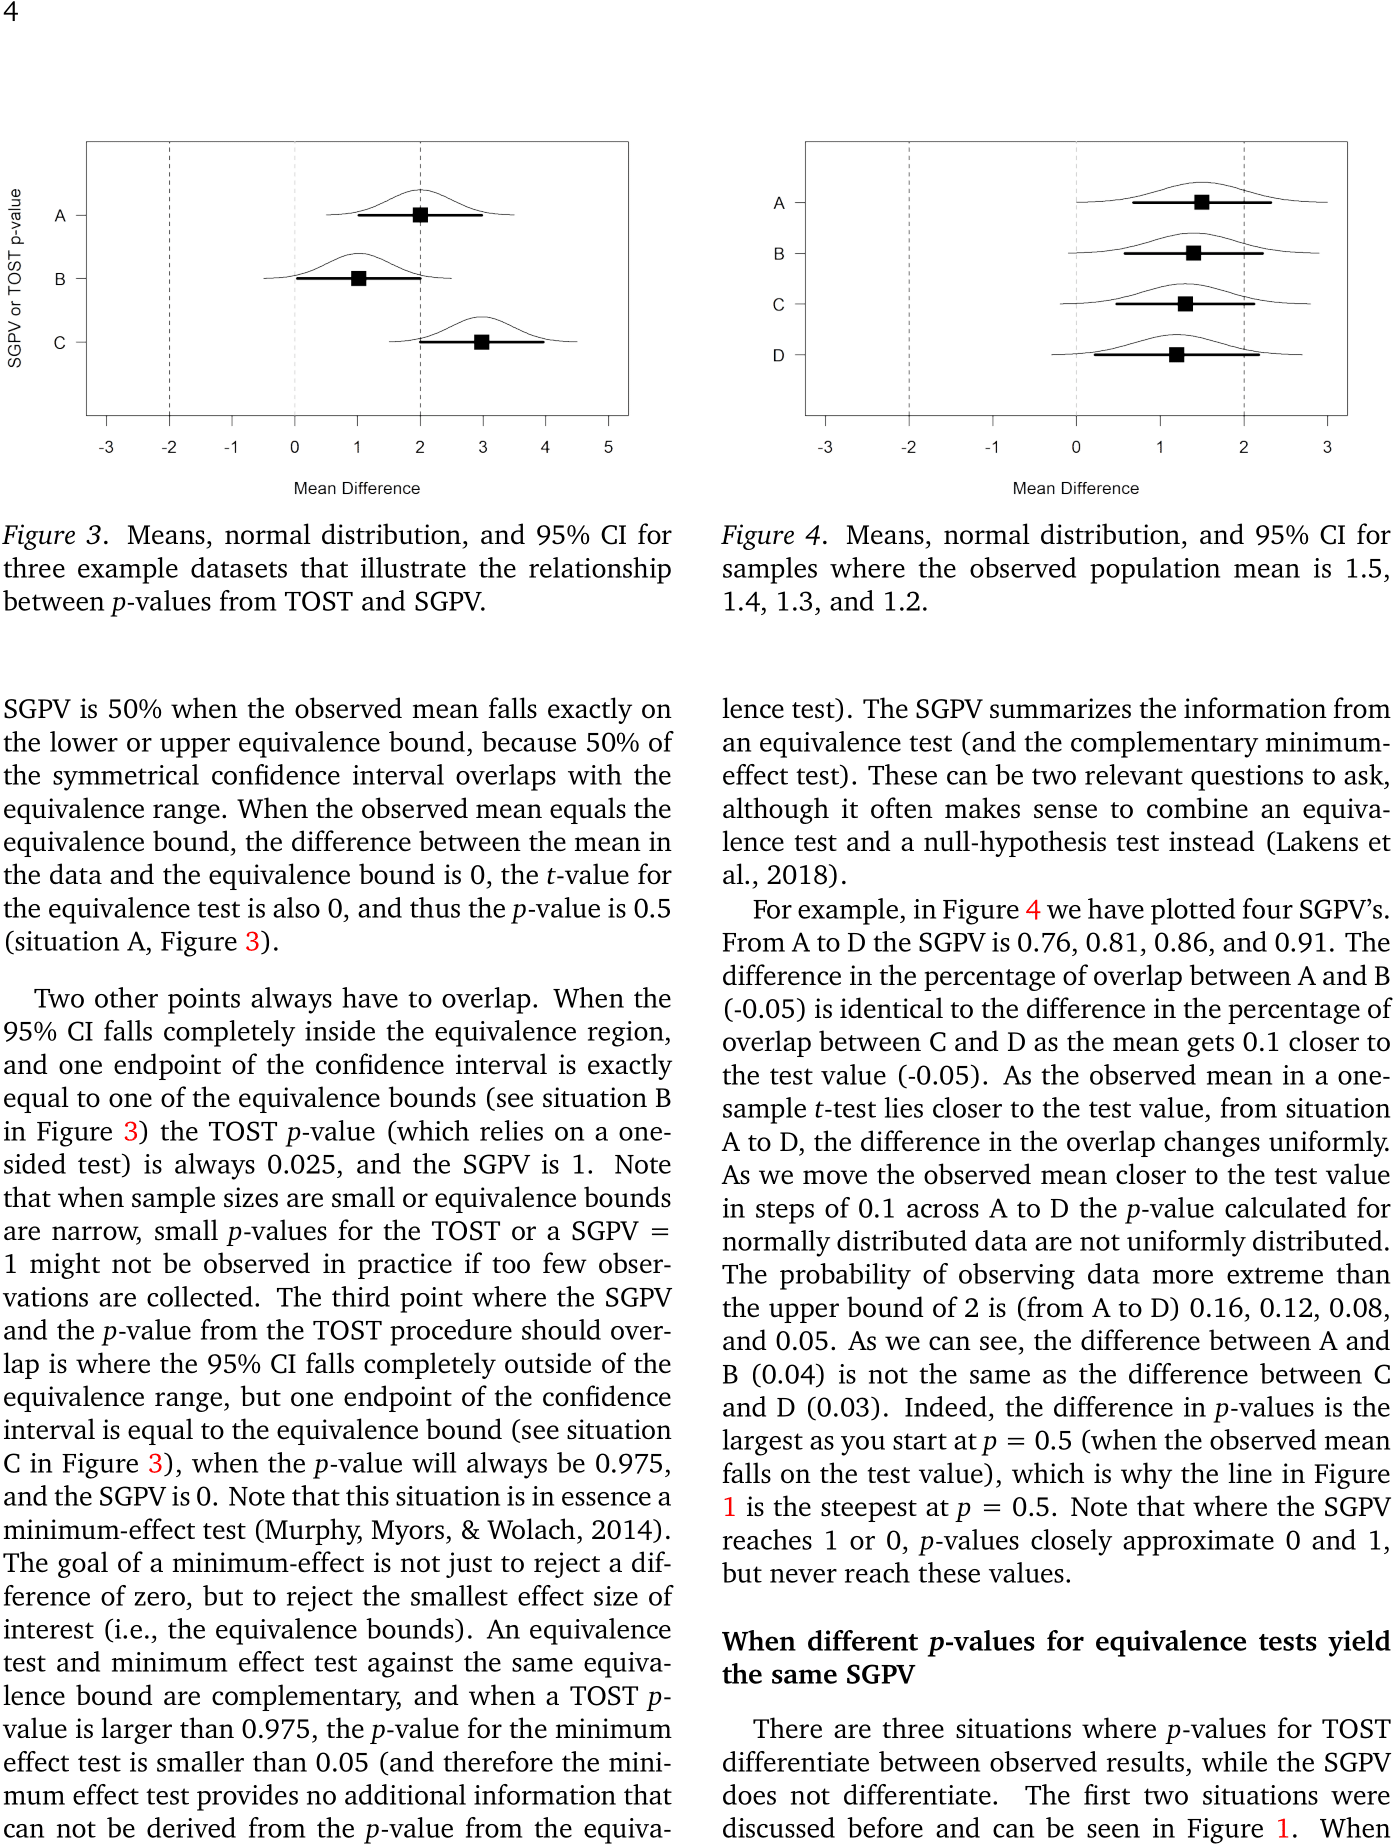
\includegraphics{C:/Users/Admin/Documents/Github projects/thesis/Chapitre 5/Chapitre 5-4} \end{center}

\begin{center}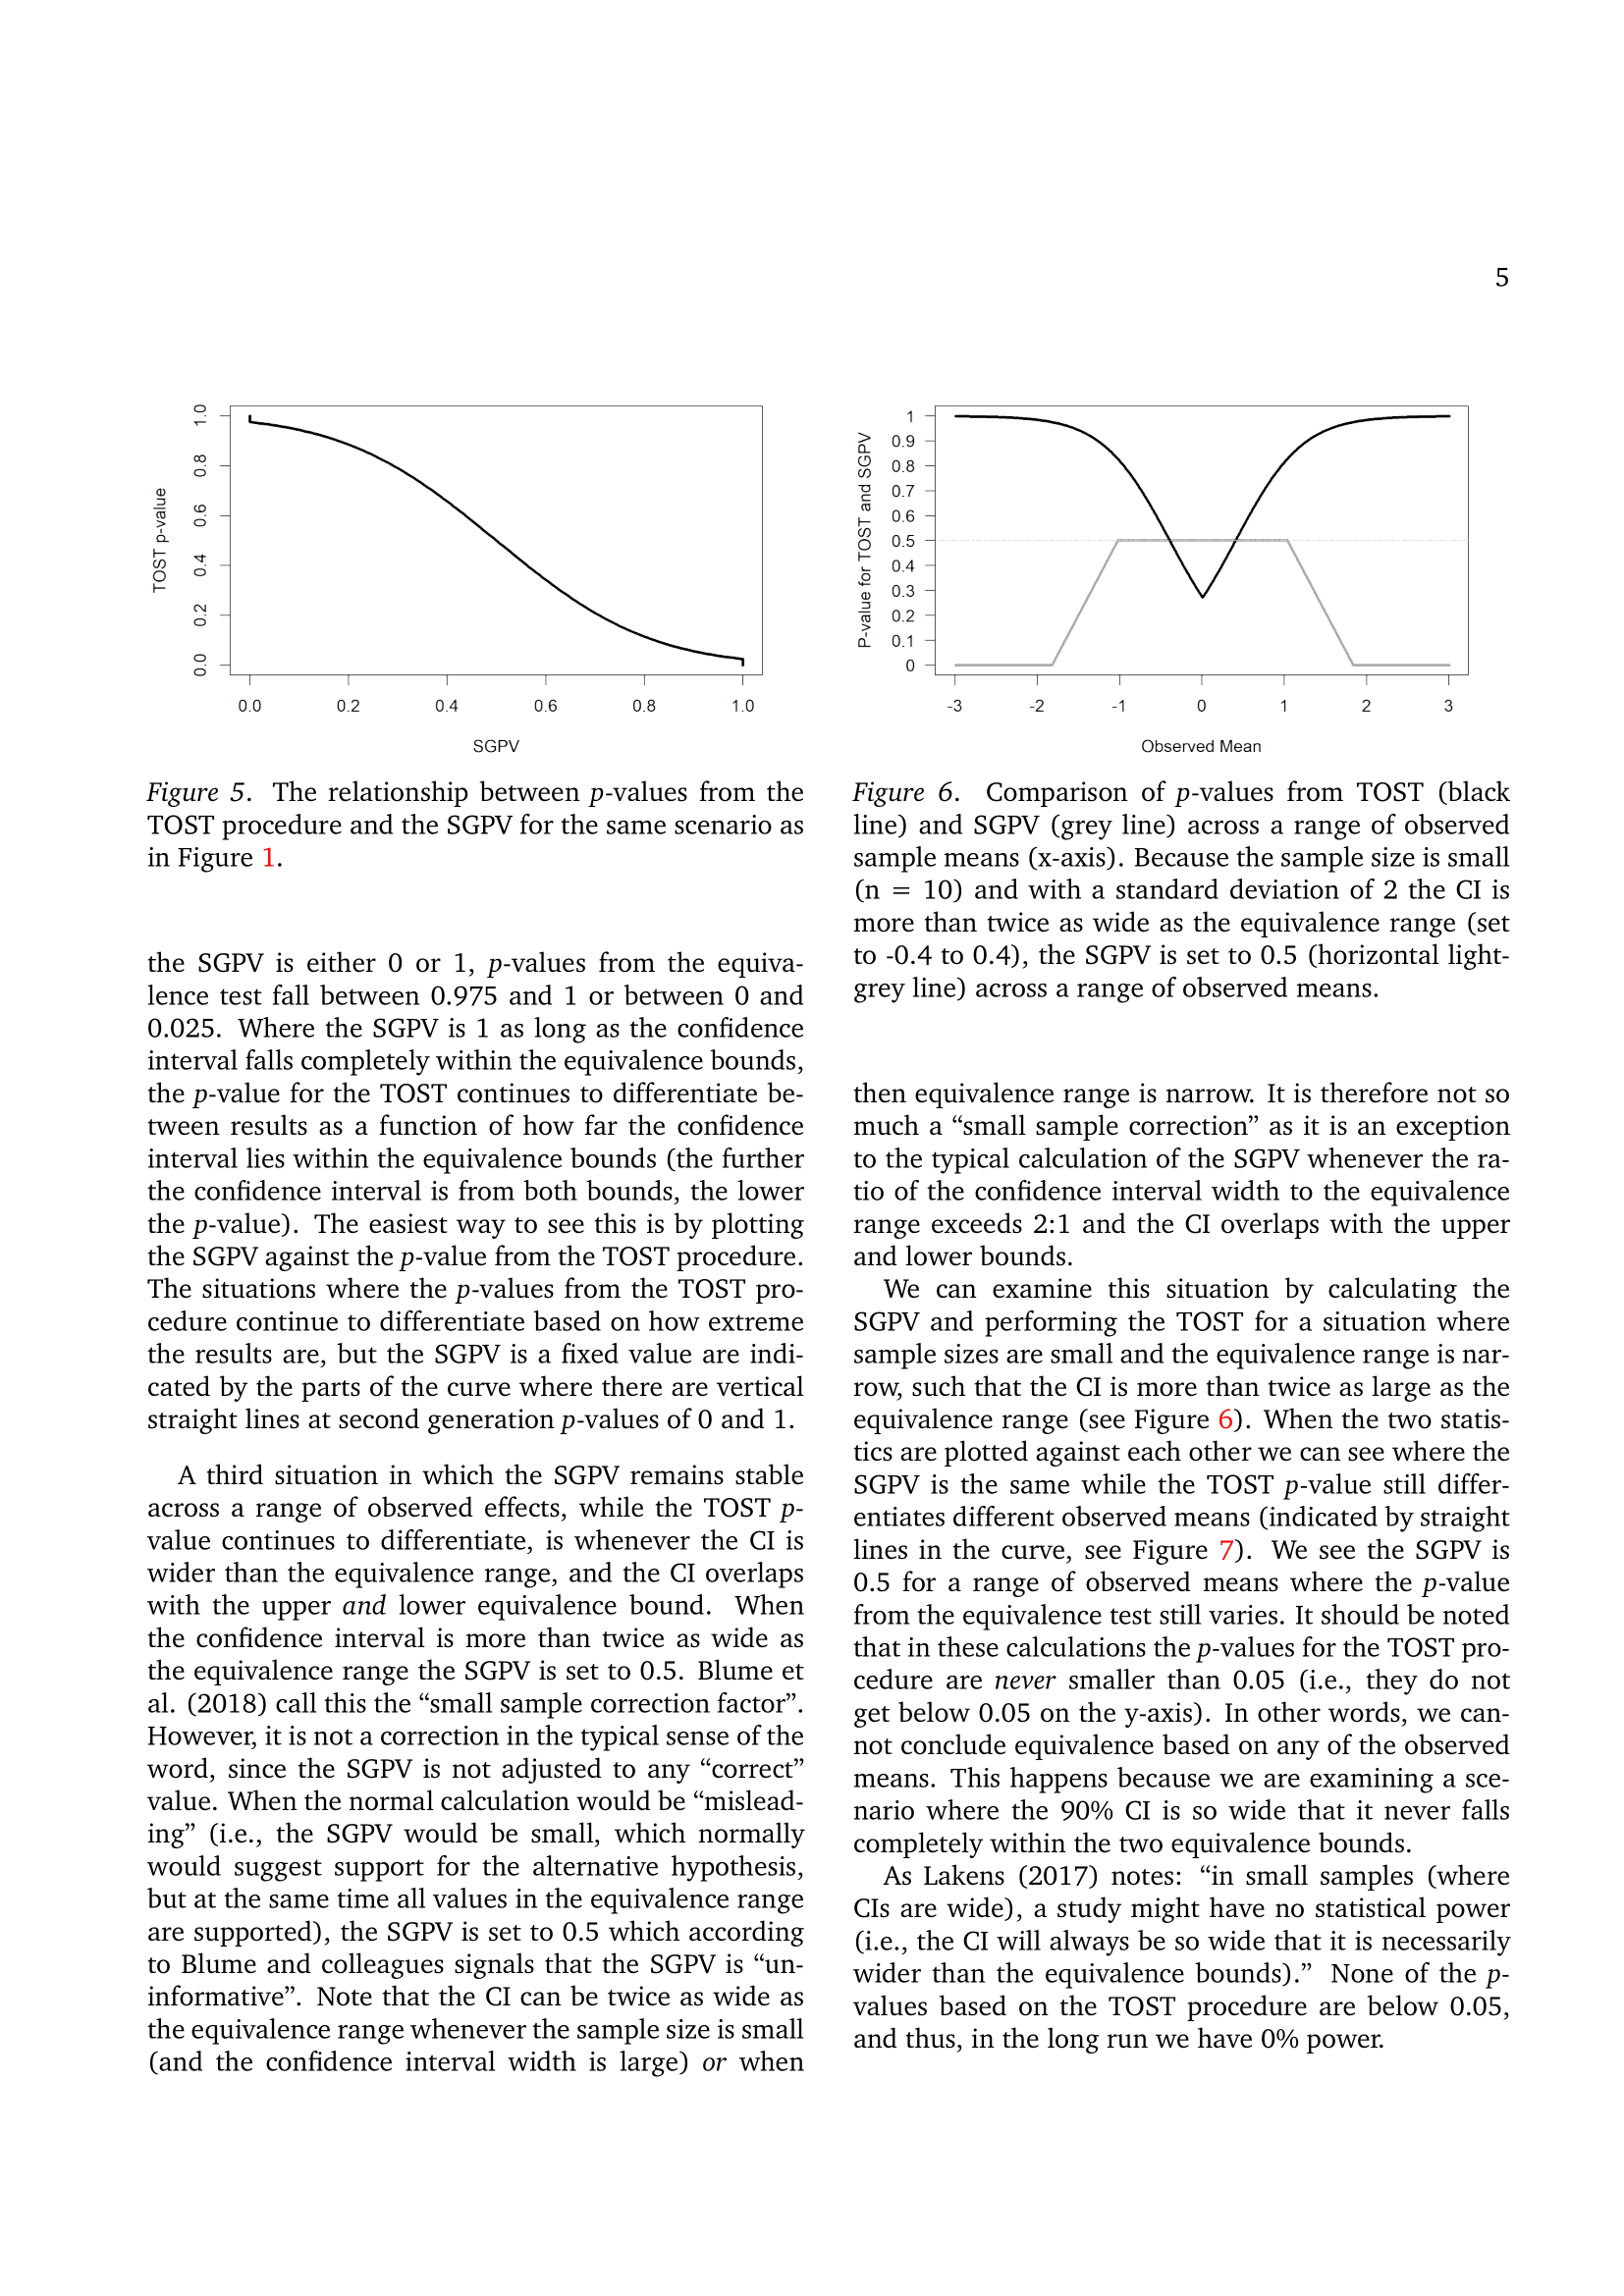
\includegraphics{C:/Users/Admin/Documents/Github projects/thesis/Chapitre 5/Chapitre 5-5} \end{center}

\begin{center}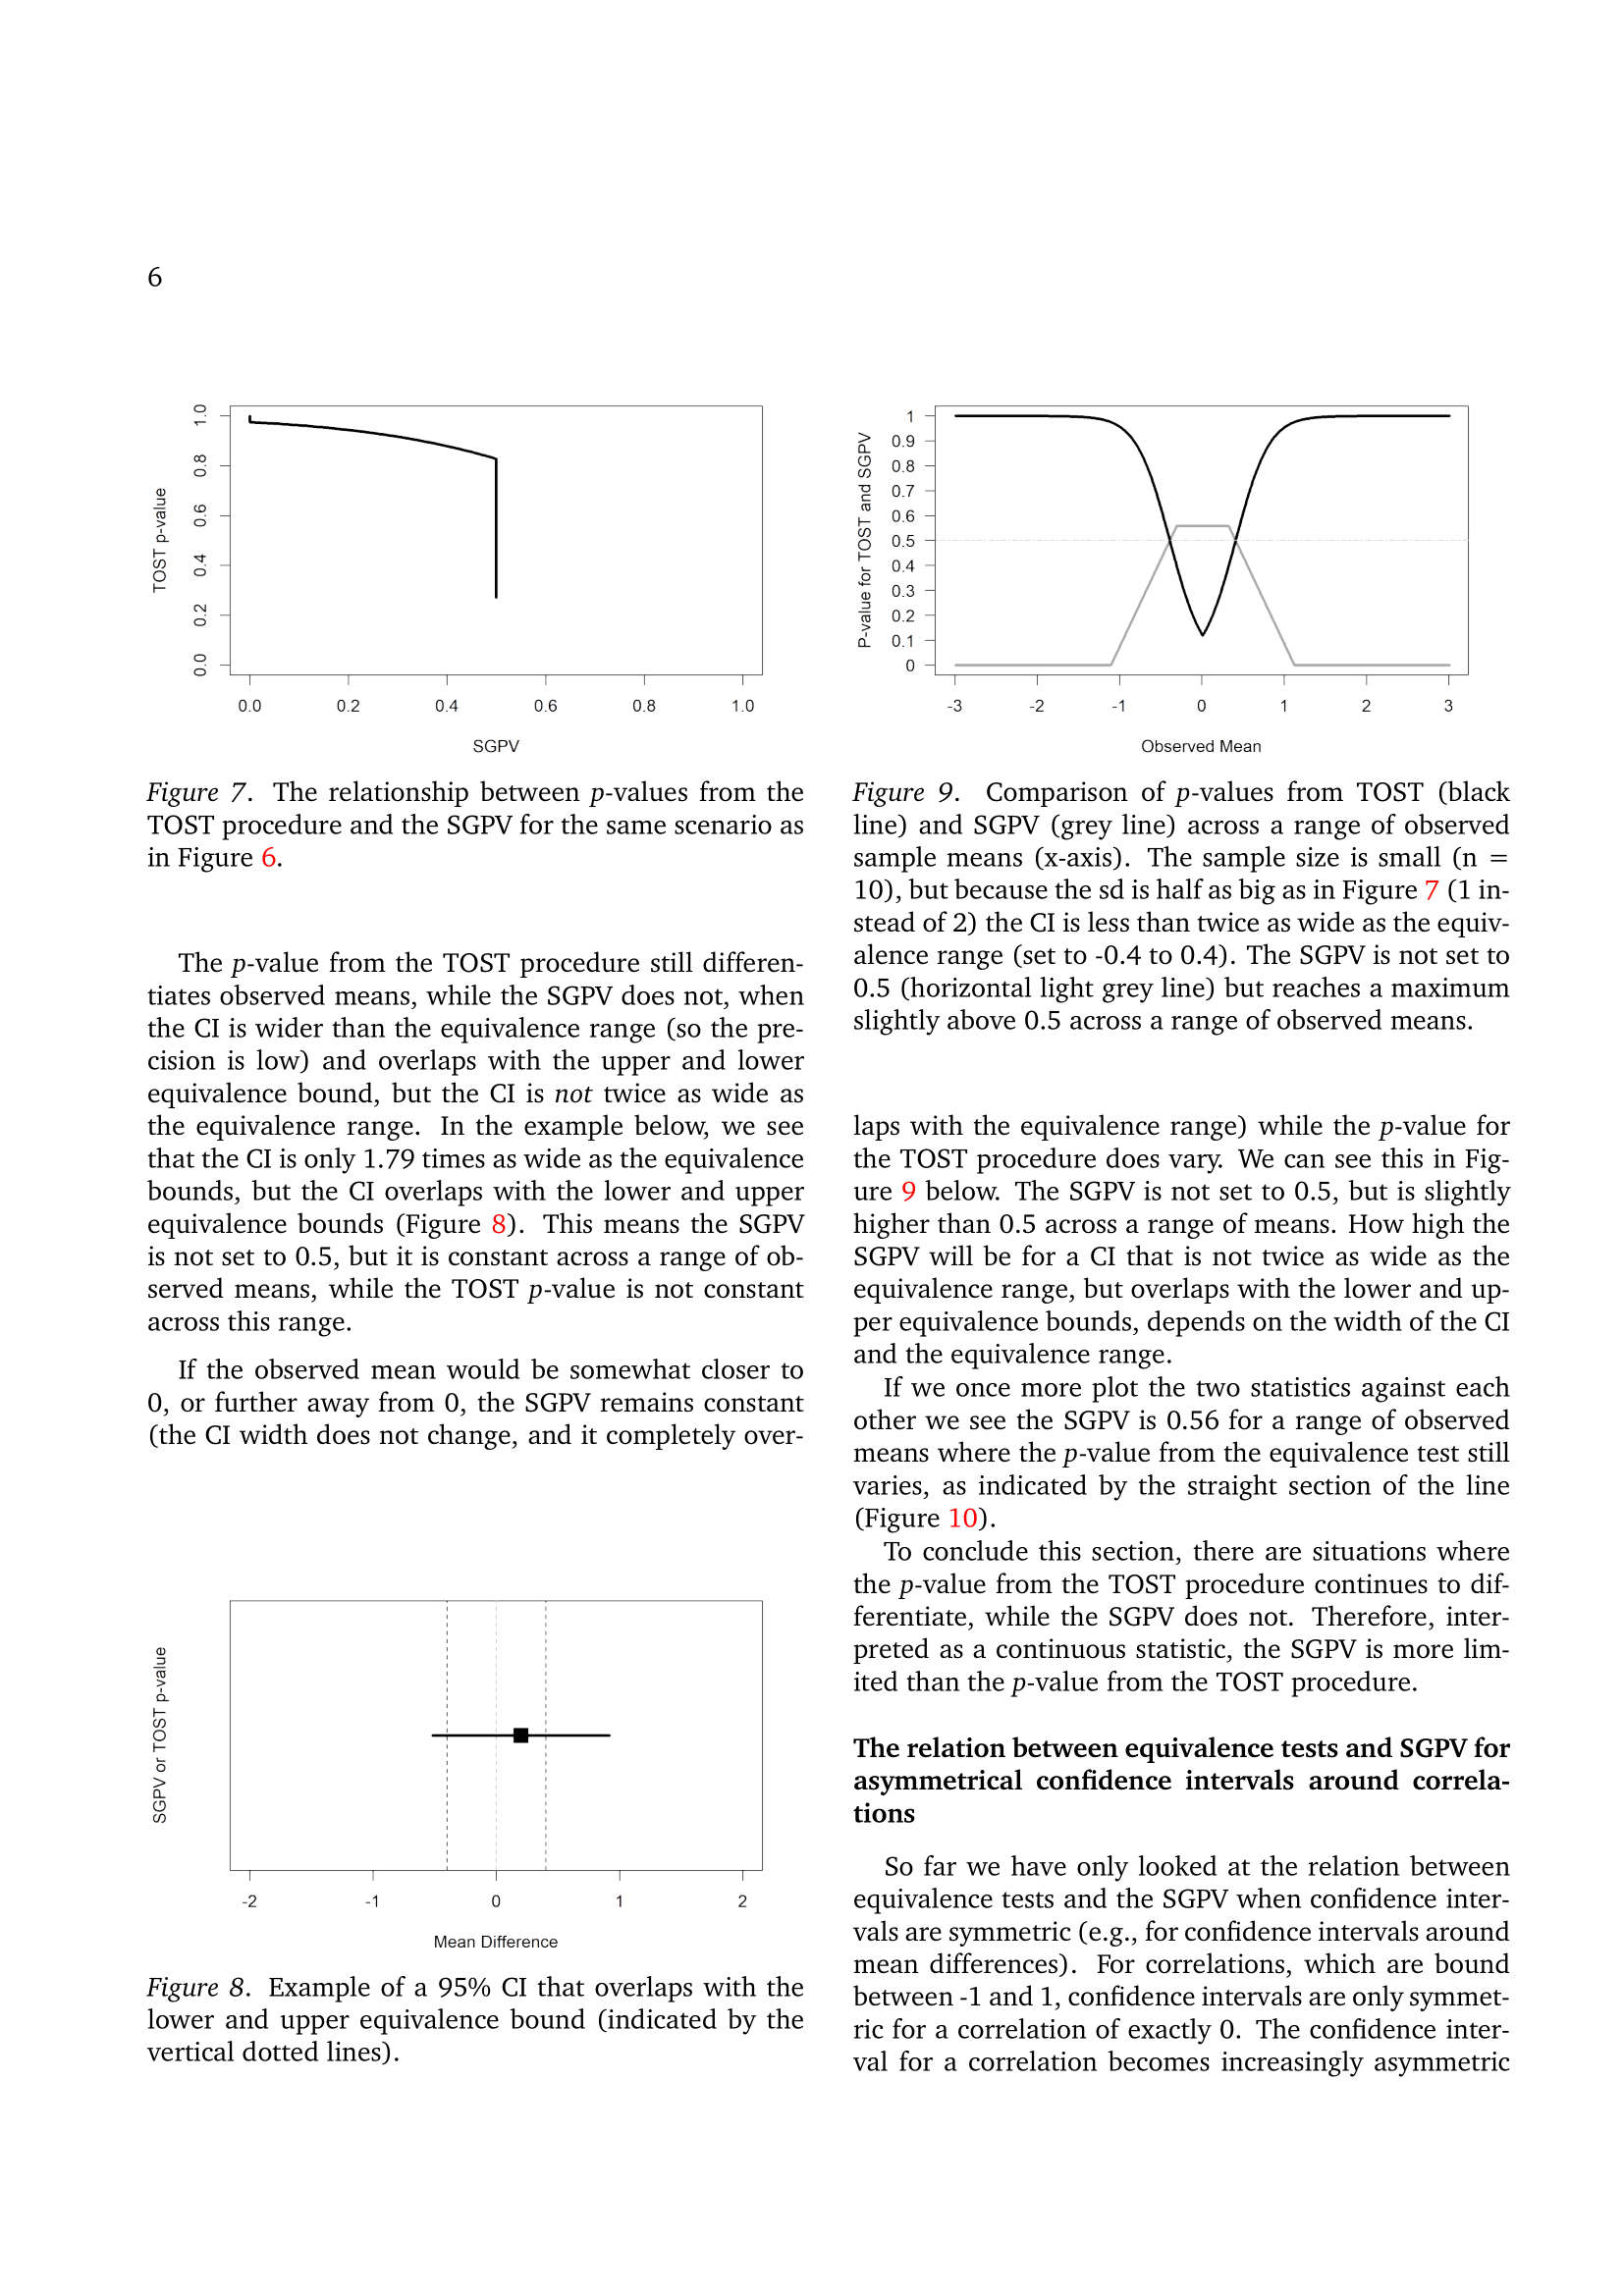
\includegraphics{C:/Users/Admin/Documents/Github projects/thesis/Chapitre 5/Chapitre 5-6} \end{center}

\begin{center}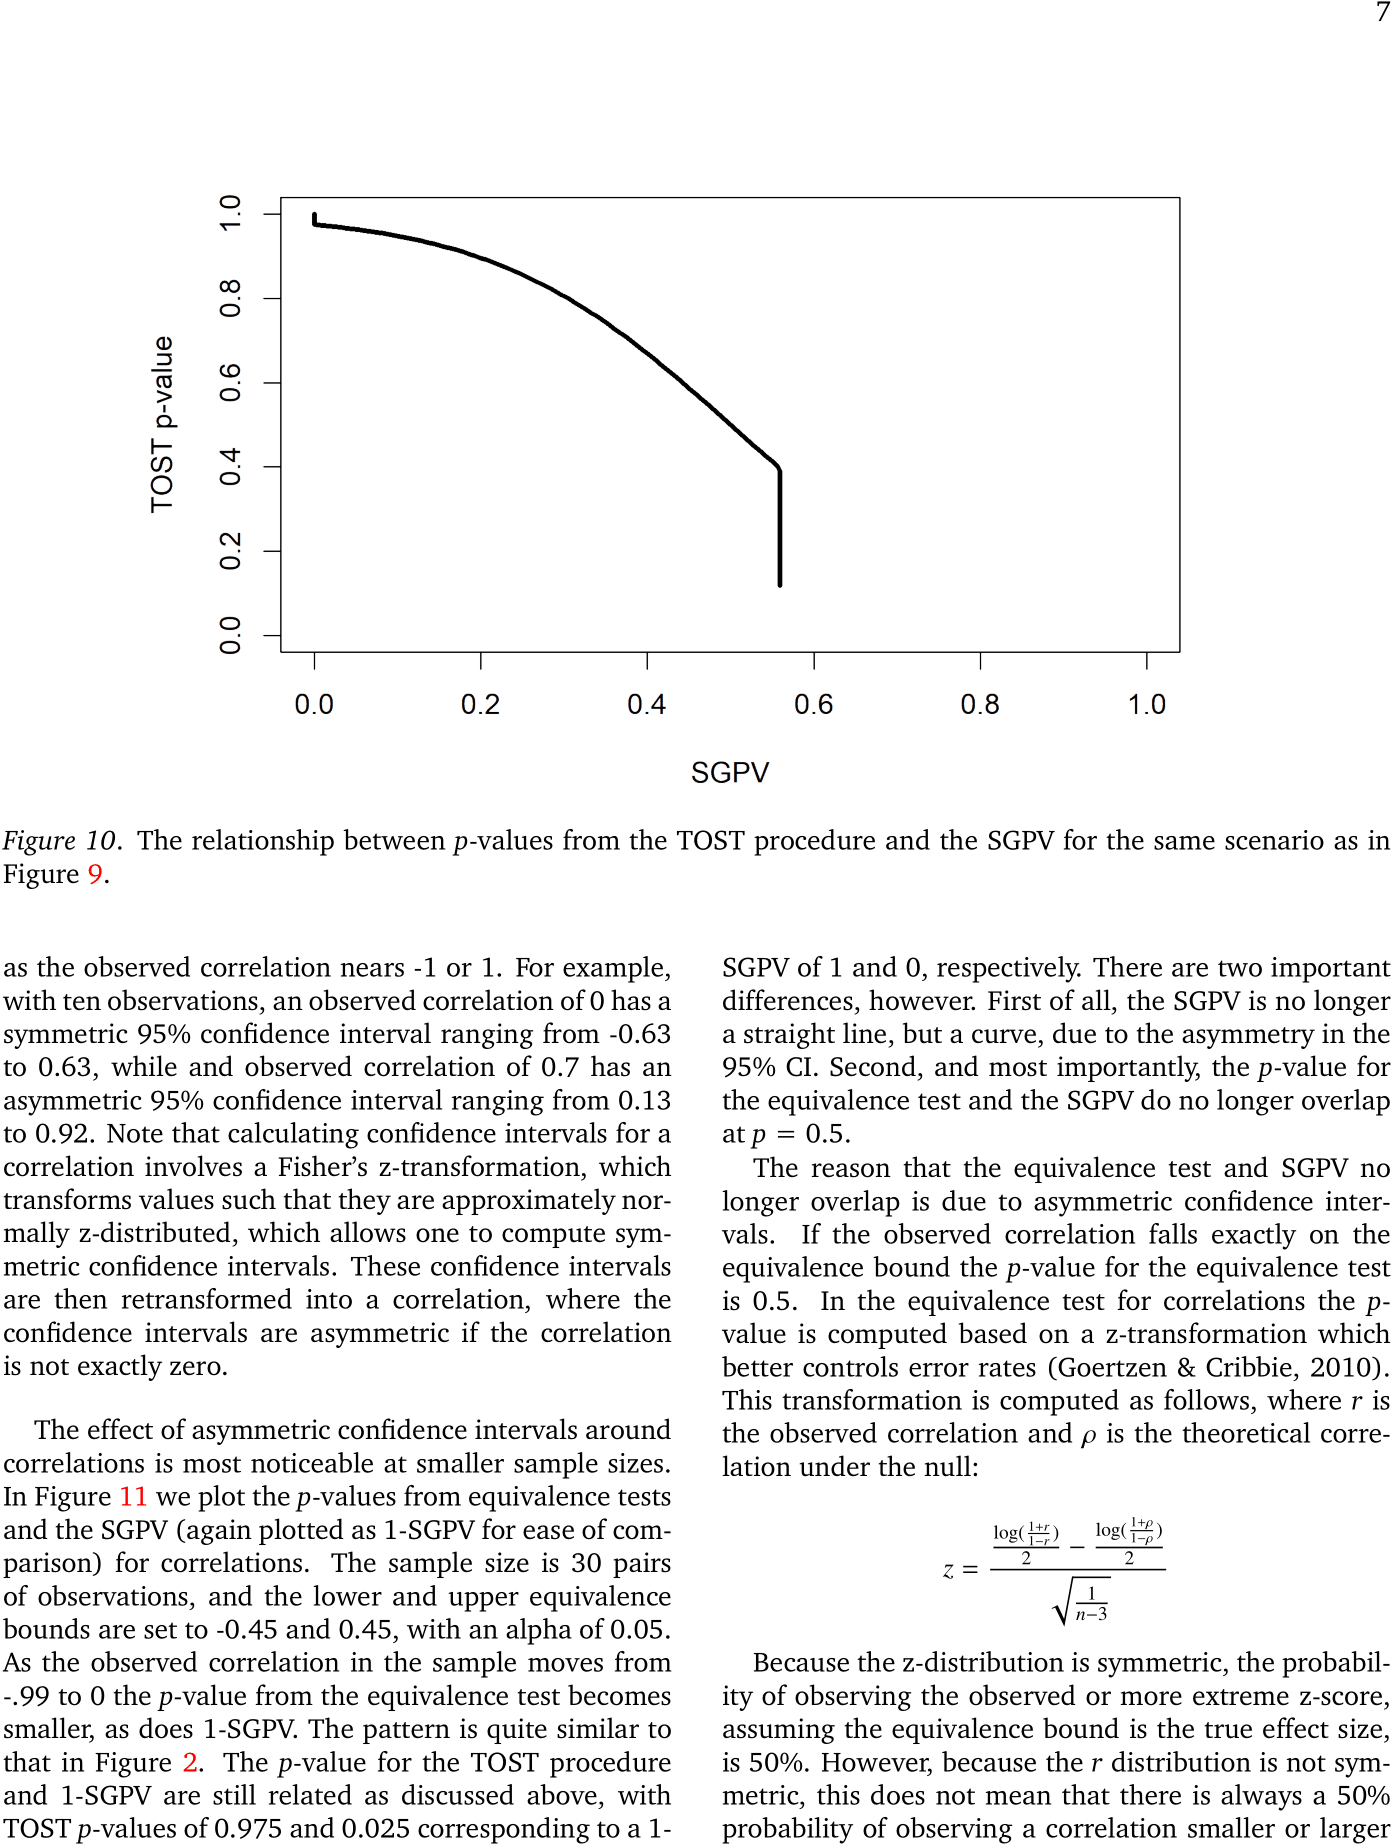
\includegraphics{C:/Users/Admin/Documents/Github projects/thesis/Chapitre 5/Chapitre 5-7} \end{center}

\begin{center}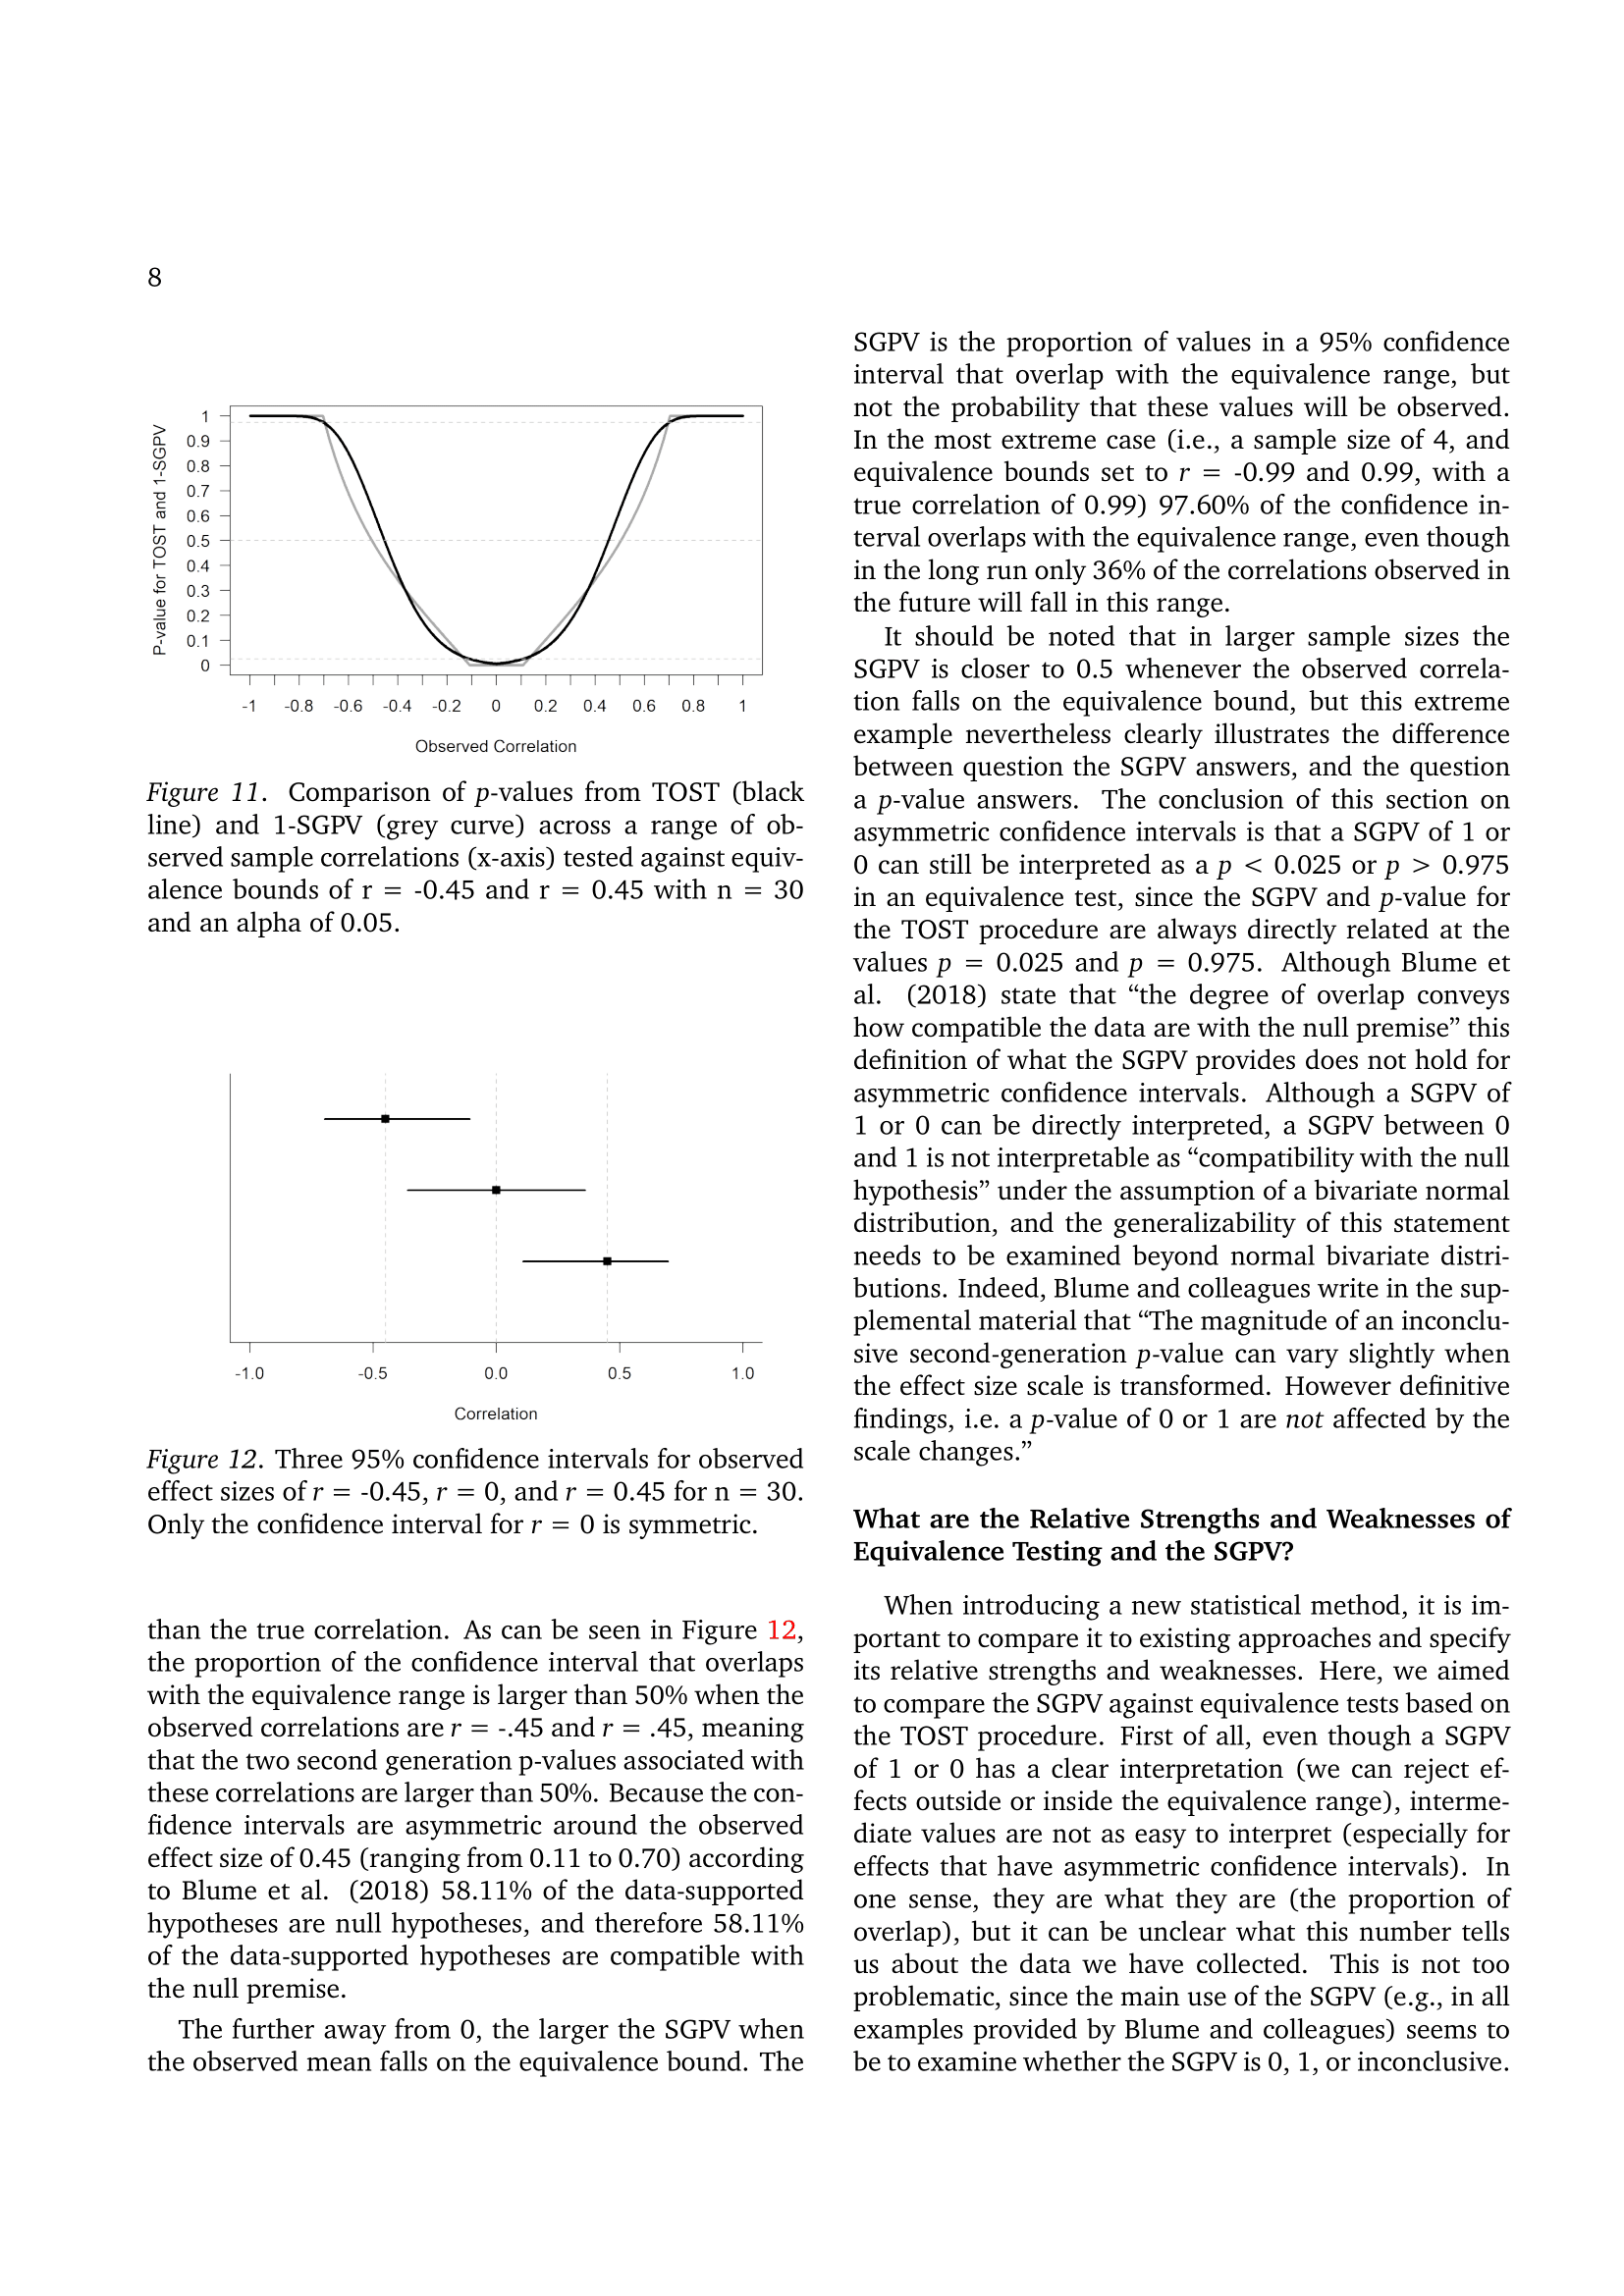
\includegraphics{C:/Users/Admin/Documents/Github projects/thesis/Chapitre 5/Chapitre 5-8} \end{center}

\begin{center}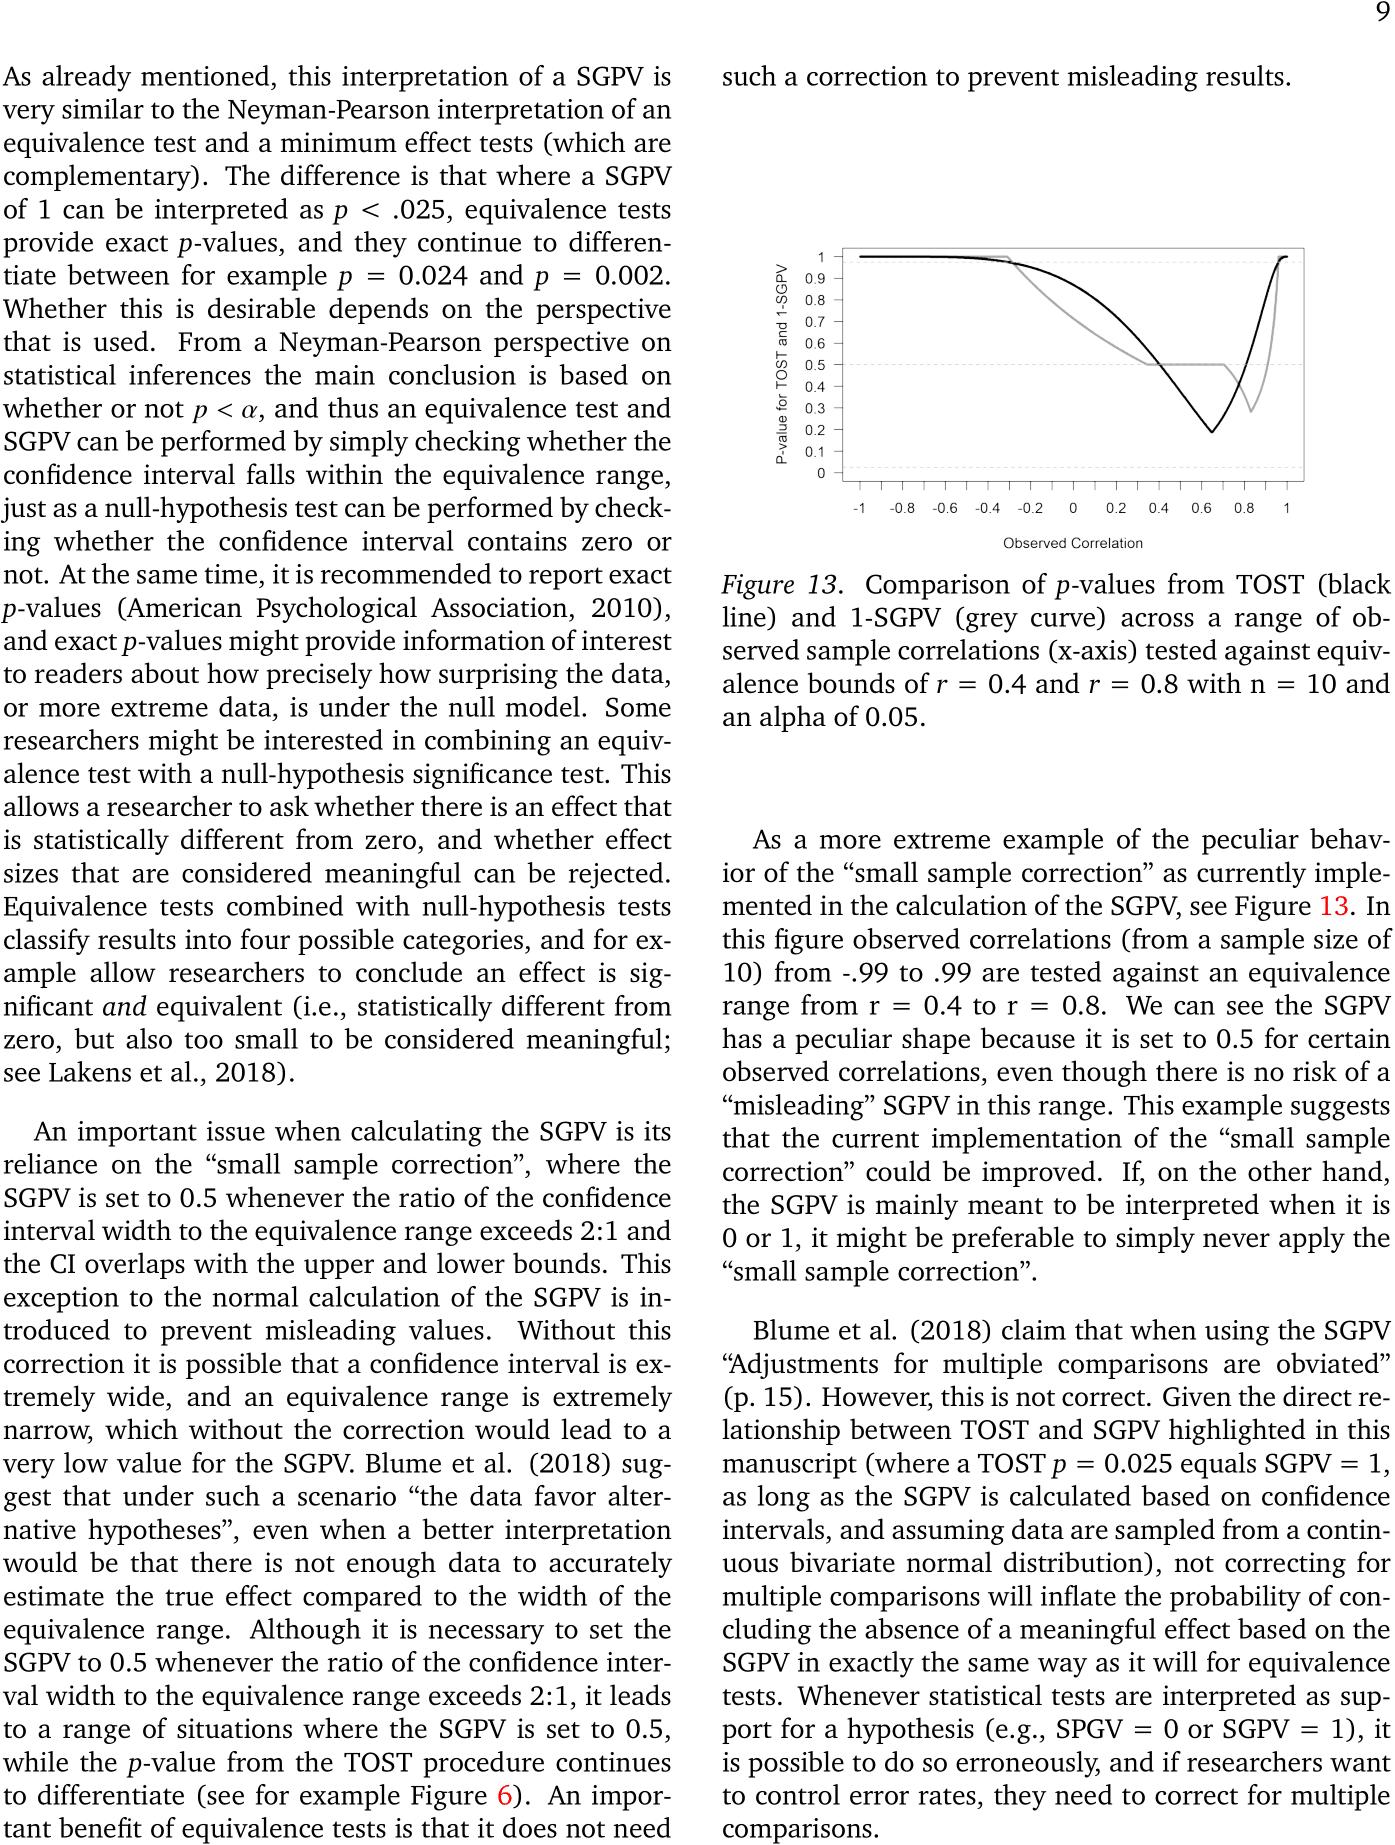
\includegraphics{C:/Users/Admin/Documents/Github projects/thesis/Chapitre 5/Chapitre 5-9} \end{center}

\begin{center}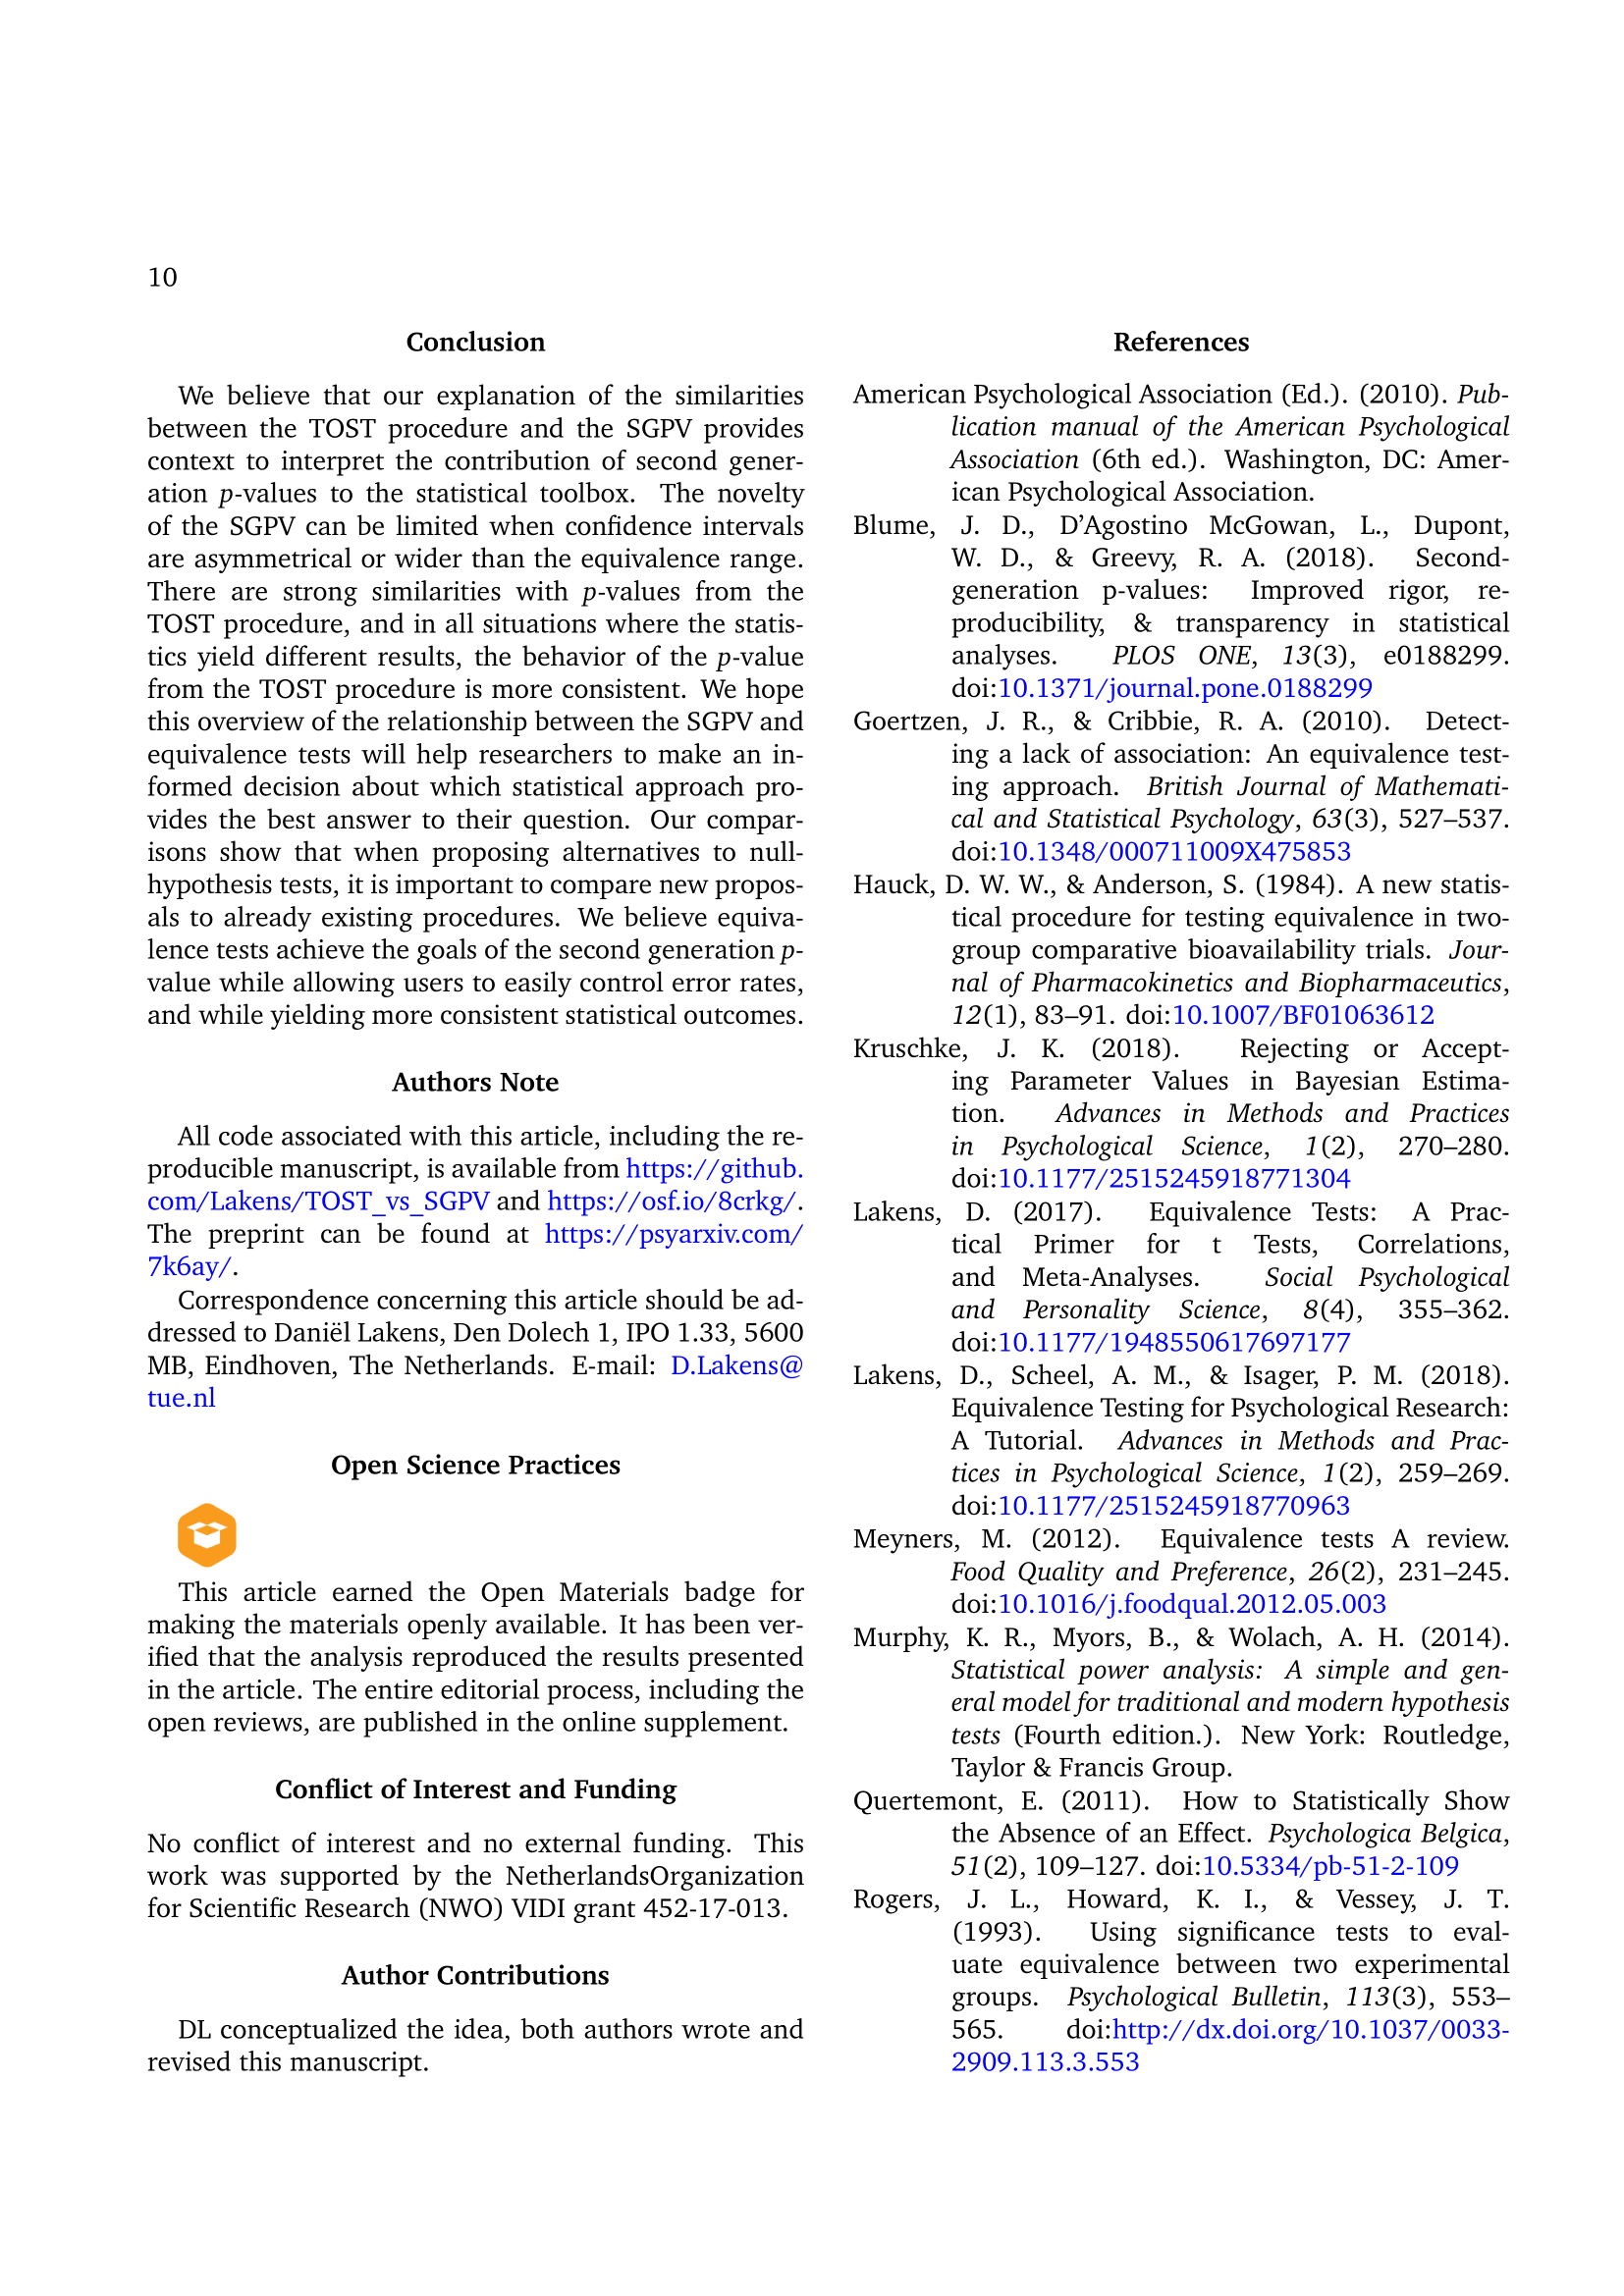
\includegraphics{C:/Users/Admin/Documents/Github projects/thesis/Chapitre 5/Chapitre 5-10} \end{center}

\begin{center}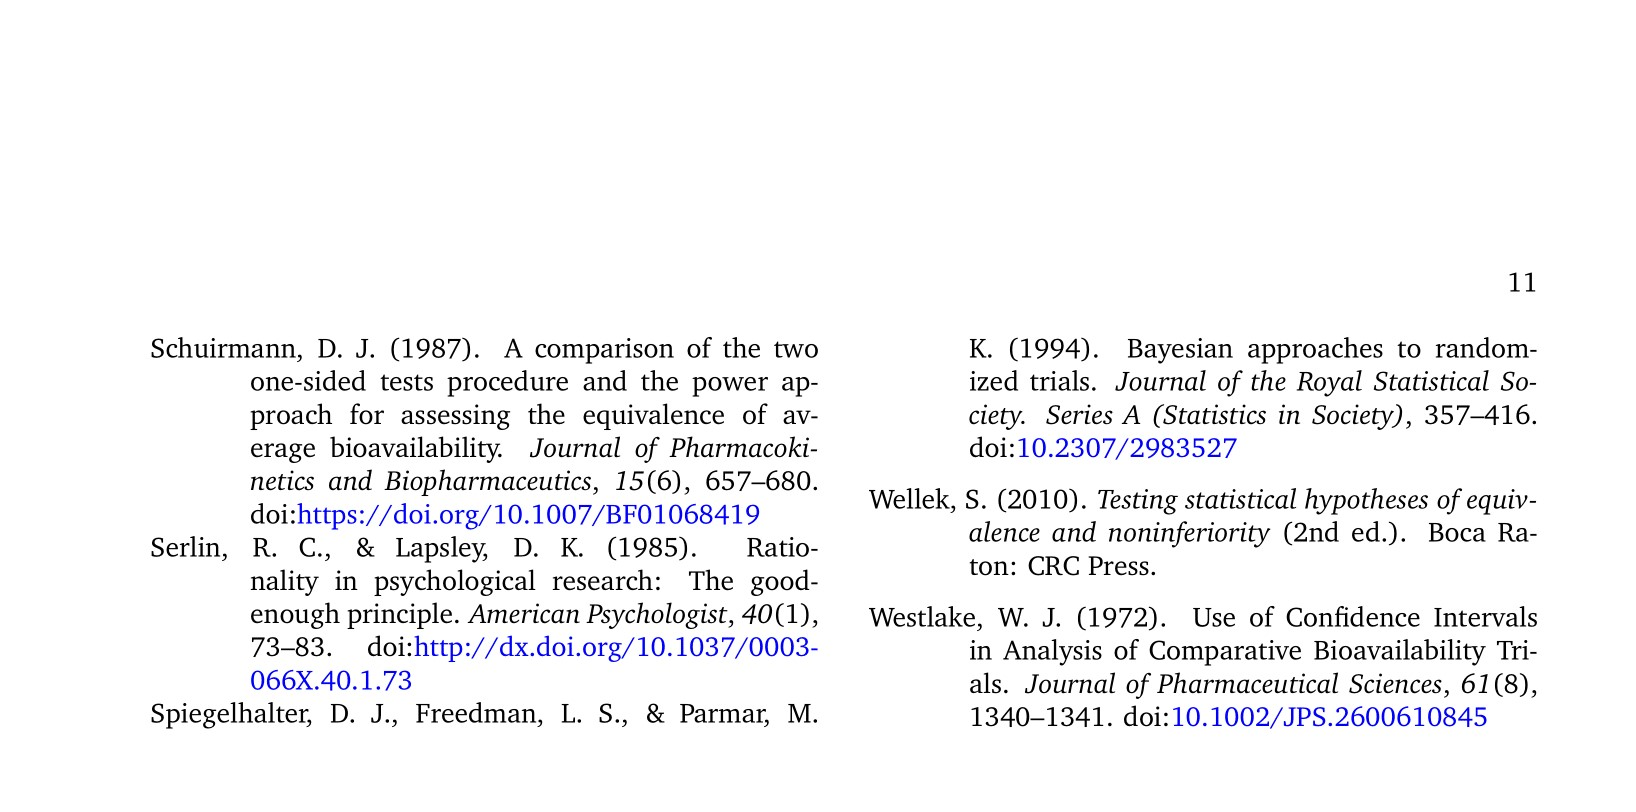
\includegraphics{C:/Users/Admin/Documents/Github projects/thesis/Chapitre 5/Chapitre 5-11} \end{center}

\parindent 0pt
\renewcommand{\notesname}{Notes de fin de chapitre}

\parskip 2ex \theendnotes \newpage

\hypertarget{discussion-guxe9nuxe9rale-et-conclusion}{%
\section{Discussion générale et
conclusion}\label{discussion-guxe9nuxe9rale-et-conclusion}}

A travers cette thèse, nos objectifs de départ étaient (1) d'identifier
des manquements dans les pratiques actuelles des chercheurs, via des
analyses d'articles publiés dans des revues de psychologie ; (2) de
réaliser des simulations, en vue de montrer l'impact de ces pratiques et
(3) de proposer des recommandations pour les améliorer.

Dans un premier temps, nous nous sommes focalisés sur l'usage des
statistiques \(t\) de Student, \(F\) de Fisher et \(d\) de Cohen, soit
des mesures communément utilisées par les chercheurs en psychologie, en
vue de comparer les moyennes de deux ou plusieurs groupes de sujets
indépendants, et qui reposent sur les conditions que des résidus,
indépendants et identiquement distribués, soient extraits d'une
distribution normale et que les variances des populations dont sont
extraits chaque groupe soient identiques (soit la condition
d'homogénéité des variances). Comme nous l'avons théoriquement décrit,
il existe toute une série d'arguments qui permettent de remettre en
cause la crédibilité des conditions statistiques de normalité (comme la
présence de sous-populations définies par des facteurs non identifiés
dans le design, l'étude de mesures bornées, telle(s?) que le temps qui
ne peut prendre des valeurs négatives, ou encore le fait qu'un
traitement est susceptible de modifier la forme des distributions
étudiées) et d'homogénéité des variances (comme l'étude de groupes
pré-existants à l'expérience, définis par des variables telles que le
genre ou l'origine
ethnique\endnote{Dans ce cas, les sujets ne sont pas répartis aléatoirement entre les groupes. L'hétérogénéité des variances entre les groupes et dès lors le résultats de la violation de la condition méthodologique d'indépendance des résidus.},
ou encore le fait qu'un traitement, qu'il soit expérimental ou
quasi-expérimental, est susceptible d'agir sur tous les paramètres d'une
distribution, incluant sa variance), dans de nombreux domaines de la
psychologie. Conformément à nos objectifs de départ, nous avons réalisé
des simulations Monte Carlo en vue de montrer les conséquences réelles
de la violation des conditions de normalité et d'homogénéité des
variances, et de comparer respectivement les statistiques \(t\) de
Student (chapitre 2), \(F\) de Fisher (chapitre 3) et \(d\) de Cohen
(chapitre 4) à des alternatives plus robustes en cas de violation de la
condition d'homogénéité des
variances\endnote{Comme expliqué en introduction, nous nous sommes principalement focalisés sur la condition d'homogénéité des variances compte tenu, d'abord, de la forte résistance de la part des chercheurs à l'égard des tests comparant d'autres indicateurs de tendance centrale que la moyenne et ensuite, du fait qu'un écart à la condition d'homogénéité des variances affectera bien plus les taux d'erreur de type I et II des statistiques $t$ de Student, $F$ de Fisher et $d$ de Cohen qu'un écart à la condition de normalité.}.
De manière consistante avec nos attentes théoriques, lorsque les deux
échantillons comparés sont de même taille, le test \(t\) de Student est
robuste aux violations de la condition d'homogénéité des variances. Par
contre, il en est différemment lorsque les échantillons sont de tailles
différentes: sur le long terme, la probabilité de rejeter l'hypothèse
nulle avec ce test est supérieure aux attentes théoriques lorsque le
plus petit échantillon est extrait de la population ayant la plus grande
variance, et est inférieure aux attentes théoriques lorsque le plus
petit échantillon est extrait de la population ayant la plus petite
variance. Au contraire, le test \(t\) de Welch ne dépend pas de la
condition d'homogénéité des variances. Il est souvent recommandé aux
chercheurs de tester préalablement la condition d'homogénéité des
variances, via un test de Levene par exemple, et ensuite d'utiliser soit
le test \(t\) de Student soit le test \(t\) de Welch, suivant que cette
condition soit ou non respectée. Cependant, dans la mesure où la
condition d'homogénéité des variances est plus souvent l'exception que
la norme et qu'il est parfois très difficile (voire impossible) de
détecter les écarts à cette condition à travers des tests, nous
recommandons l'usage du test \(t\) de Welch par défaut, au moins lorsque
les échantillons sont de taille différente. En effet, ce test est
pratiquement aussi puissant que le test \(t\) de Student lorsque la
condition d'homogénéité des variances est respectée, et contrôle bien
mieux les taux d'erreur de type I et II lorsqu'elle ne l'est pas. Par
ailleurs, il est disponible dans presque tous les logiciels statistiques
courants (\(R\), Minitab, Jamovi, SPSS, etc.). Dans la mesure où l'ANOVA
\(F\) de Fisher est une généralisation du test \(t\) de
Student\endnote{L'ANOVA $F$ de Fisher peut être utilisée lorsqu'on compare deux ou plus de deux échantillons indépendants sur base de leur moyenne. Lorsqu'on compare exactement deux groupes, le test $t$ de Student et l'ANOVA $F$ de Fisher sont strictement équivalents. En effet, ils entretiennent la relation mathématique suivante: $F(1,x) = t^2(x)$.},
il n'est pas surprenant que nos simulations relatives à l'ANOVA \(F\) de
Fisher amènent à des constats semblables à ceux obtenus sur base de nos
simulations relativement au test \(t\) de Student. En outre, ces
simulations nous ont permis de faire deux constats supplémentaires:
d'abord, lorsqu'on compare plus de deux groupes, l'ANOVA \(F\) de Fisher
est affectée par la présence d'hétérogénéité des variances, même lorsque
tous les échantillons sont de tailles identiques. Dans ce cas, le test
devient plus liberal, ce qui signifie qu'il amène à rejeter l'hypothèse
nulle plus souvent qu'attendu théoriquement, sur le long terme. Ensuite,
plus le nombre d'échantillons comparés est important, plus le test est
affecté par les violations de la condition d'homogénéité des variances.
En cas d'homogénéité des variances, le test \(W\) de Welch est très
légèrement inférieur aux tests \(F^*\) de Brown-Forsythe que \(F\) de
Fisher, tant en termes de contrôle des erreurs de type I et II qu'en
termes de consistances entre les puissances théoriques et observées. Par
contre, il leur est bien supérieur en cas d'hétérogénéité des variances.
Pour les mêmes raisons que celles qui nous amènent à privilégier le test
\(t\) de Welch par défaut, nous recommandons de privilégier
systématiquement le test \(W\) de Welch lorsqu'on compare plus de deux
groupes de sujets indépendants sur base de leur moyenne. Tout comme le
test \(t\) de Welch, le test \(W\) de Welch est disponible dans la
plupart des logiciels statistiques fréquemment utilisés par les
chercheurs en psychologie (\(R\), Minitab, Jamovi, SPSS, etc.). En ce
qui concerne la mesure \(d\) de Cohen, nous avons mis deux éléments
principaux en évidence. D'abord, il s'agit d'une mesure toujours
biaisée, même lorsque toutes les conditions dont elle dépend sont
respectées. Heureusement, une transformation de cette mesure existe
telle que le biais devient nul lorsque la condition de normalité des
résidus est respectée. Cette transformation a été proposée par Hedges et
porte dès lors son nom: la mesure \(g\) de Hedges. Ensuite, une
violation de la condition d'homogénéité des variances amènera à une
forte augmentation de la variance des estimateurs \(d\) de Cohen et
\(g\) de Hedges, même lorsque les deux échantillons sont de taille
identique. Différents estimateurs ont été proposés dans la littérature
en vue de remplacer le \(d\) de Cohen (et le \(g\) de Hedges) en cas de
violation de la condition d'homogénéité des variances. Parmis ceux-ci,
on retrouve fréquemment le \(d\) de Glass, qui peut être transformé de
sorte à obtenir le \(g\) de Glass, théoriquement non biaisé lorsque les
résidus se distribuent normalement. Nos simulations ont révélé que la
variance du \(g\) de Glass de même que son biais (lorsque les résidus
sont extraits de populations qui ne se distribuent pas normalement)
dépendent fortement de paramètres que l'on ne peut contrôler, ce qui
nous amène à décourager l'usage de cette mesure. Dans la litérature, on
retrouve également la mesure \(d\) de Shieh, qui entretient une relation
mathématique directe avec le \(t\) de Welch, ainsi que la mesure \(d^*\)
de Cohen qui, contrairement au \(d\) de Cohen classique, implique le
calcul de la moyenne \emph{non poolée} des variances de chaque groupe.
De même que pour les estimateurs précédemment cités, il est possible de
transformer ces mesures en vue de supprimer le biais lorsque la
condition de normalité des résidus est respectée. Cela donne
respectivement lieu aux mesures \(g^*\) de Hedges et \(g\) de Shieh.
Grâce à nos simulations, nous avons révélé que le \(g^*\) de Hedges est
supérieur au \(g\) de Shieh, non seulement d'un point de vue inférentiel
(contrairement au \(g\) de Shieh, le \(g^*\) de Hedges est consistant,
ce qui signifie que sa variance diminue toujours lorsque les tailles
d'échantillon augmentent, de même que son biais lorsque les résidus sont
extraits d'une population anormale) que d'un point de vue interprétatif
(sa valeur est constante, peu importe que les deux échantillons soient
de taille identique ou non). Finalement, lorsqu'on compare les mesures
\(g\) de Hedges et \(g^*\) de Hedges, on constate que le \(g^*\) de
Hedges n'est très légèrement inférieur au \(g\) de Hedges, en termes de
biais et de variance, que lorsque des échantillons de tailles
différentes sont extraits de population aux variances identiques. Il est
tout aussi efficace que le \(g\) de Hedges lorsque tant les tailles
d'échantillons que les variances de population sont identiques. De plus,
il reste valide lorsque la condition d'homogénéité des variances n'est
pas respectée, contrairement au \(g\) de Hedges. Pour les mêmes raisons
que celles qui nous amènent à privilégier les tests \(t\) de Welch et
\(F\) de Welch par défaut, nous recommandons de privilégier
systématiquement le \(g^*\) de Hedges.

\color{red}: si j'insérais plutôt les apports ici?

\color{blue}Bien que la question de l'impact des violations des
conditions d'application des tests \(t\) de Student et \(F\) de Fisher
ait déjà été largement explorée par les méthodologistes (voir par
exemple Harwell, 1992), ces débats semblaient toujours ignorés par de
nombreux chercheurs appliqués. Il nous est apparu que la litérature
manquait d'articles expliquant de manière accessible les conséquences
réelles de ces violations, en s'appuyant sur des exemples concrets et
issus de la psychologie. Notre principale mission, lors de la rédaction
des articles présentés au sein des chapitre 2 et 3 de cette thèse, était
d'ordre pédagogique. Nous visions à réduire le fossé entre les
méthodologistes ayant des connaissances statistiques très pointues et
les autres chercheurs appliqués. Par ailleurs, les moyens informatiques
actuels nous ont permis de généraliser les conclusions tirées par
d'autres chercheurs avant nous, grâce à la réalisation de simulations
intensives, avec 1,000,000 d'itérations pour plusieurs milliers de
scénarios qui variaient en fonction d'un ensemble de paramètres connus
pour jouer un rôle clé sur les taux d'erreur de type I et II des tests
\(t\) de Student et \(F\) de Fisher.

Afin d'augmenter l'impact de ces articles, d'un point de vue
pédagogique, nous avons tenté de rendre notre recherche la plus
tranparente possible et surtout, de la diffuser à grande échelle.
Plusieurs démarches ont été faites en ce sens: 1) Nous avons
systématiquement diffusé des preprint, chaque fois que nous avons soumis
un article. \emph{Cette pratique a eu des retombées positives qui ont
dépassé nos attentes, grâce à la collaborations d'éminents chercheurs
(exemple du dernier article qui a été très longuement commenté par
Cumming), }\\
2) Nous avons systématiquement privilégié des revues Open Access
(\emph{International Review of Social Psychology}, \emph{British Journal
of Mathematical and Statistical Science}, \emph{AMPPS}).\\
3) Nous avons utilisé Github.\\
Le taux élevé de citation de nos articles semble attester de notre
réussite à atteindre cet objectif.

\color{brun} Pour assurer l'impact d'un article pédagogique, il est
important de pouvoir comprendre les procédures et méthodes requises par
les psychologues afin de s'adapter aux mieux à leurs besoins et
attentes, et c'est pourquoi, à l'instar de Golinski \& Cribbie (2009),
il nous semblait important que ce travail soit réalisé par une équipe
incluant des psychologues ayant une expérience dans la recherche
appliquée, ce qui était le cas de deux des co-auteurs (Daniël Lakens et
Christophe Leys). Cette conscience de la réalité des psychologues est
vraisemblablemnet ce qui nous a amené à recommander l'usage du test de
Welch plutôt que l'usage de tests bien plus complexes qui avaient peu de
chances de susciter l'adhésion des chercheurs.

Dans un deuxième temps, nous nous sommes concentrés sur la tendance des
chercheurs à définir par défaut, comme hypothèse nulle, une hypothèse
d'absence d'effet. Nous avons souligné que cette tendance persiste même
lorsque l'objectif est de prouver une absence d'effet: c'est alors sur
base d'un non rejet de l'hypothèse nulle que les chercheurs affirment
pouvoir valider leur hypothèse. Pourtant, nous avons vu que ce n'est pas
une stratégie adéquate puisque non seulement le test utilisé de cette
manière présente de faibles propriétés asymptotiques, mais en plus, la
probabilité que le test amène à conclure à l'absence d'effet augmente à
mesure que l'erreur de mesure augmente. Nous avons également souligné
qu'en réalité, il n'existe aucun test d'hypothèses qui permette de
démontrer l'absence totale d'effet. Par contre, il est possible de
démontrer qu'un effet observé ne s'éloigne pas de l'absence d'effet
d'une quantité supérieure à une valeur définie (dit autrement, qu'il est
\emph{équivalent}), à condition de comprendre qu'il est théoriquement
possible de définir n'importe quelle différence (ou intervalle de
différences) de moyennes comme hypothèse nulle. C'est le principe sur
lequel repose le TOST (Two One-Sided Tests), à travers lequel on conclut
à l'équivalence à condition que l'intervalle de confiance à
\((1-2\alpha)\%\) autour de l'effet étudié soit entièrement inclus à
l'intérieur de la zone d'équivalence. Récemment, Blume, D'Agostino
McGowan, Dupont, Greevy, \& Robert (2018) ont proposé un nouvel outil
qui se nomme le SGPV (Second Generation P-Value) qu'ils définissent
comme la proportion des valeurs de l'intervalle de confiance à
\((1-\alpha)\%\) qui sont également compatibles avec l'hypothèse nulle
(ou autrement dit, qui se situent à l'intérieur de la zone
d'équivalence). Il nous a semblé pertinent de comparer le SPGV au TOST,
dans la mesure où les deux stratégies reposent sur un principe
similaire, à savoir la comparaison de l'intervalle de confiance de
l'effet observé avec la zone d'équivalence. Cependant, notre comparaison
n'a pas permis de mettre en évidence de réelle plus-value du SGPV par
rapport au TOST. Bien que Blume, D'Agostino McGowan, Dupont, Greevy, \&
Robert (2018) présentent le SGPV comme un outil permettant de déterminer
à quel degré les données sont compatibles avec l'hypothèse
d'équivalence, nous avons révélé au moins deux situations pour
lesquelles cette définition ne tient pas: lorsque l'intervalle de
confiance autour de l'effet observé recouvre les deux bornes de la zone
d'équivalence tout en ayant une largeur moins de deux fois supérieure à
celle de la zone d'équivalence, et lorsque les intervalles de confiance
sont asymétriques, ce qui est le cas, par exemple, lorsqu'on étudie une
corrélation \(r\) de Pearson (tel que décrit dans l'article du chapitre
5) ou encore lorsqu'on étudie des mesures de taille d'effet
standardisées de la famille \(d\) (ces dernières ayant fait l'objet du
chapitre 4). In fine, les seules situations pour lesquelles le SGPV
permet de tirer une conclusion claire sont celles où sa valeur vaut
exactement 0 ou 1. Or, les conclusions tirées dans ce cas sont
similaires, mais moins précises, à celles que permettent de tirer le
TOST.

\hypertarget{apports-thuxe9oriques-et-appliquuxe9s}{%
\subsection{Apports théoriques et
appliqués}\label{apports-thuxe9oriques-et-appliquuxe9s}}

\hypertarget{chapitres-2-et-3-test-t-de-student-et-f-de-fisher}{%
\subsubsection{\texorpdfstring{Chapitres 2 et 3 (test \(t\) de Student
et \(F\) de
Fisher)}{Chapitres 2 et 3 (test t de Student et F de Fisher)}}\label{chapitres-2-et-3-test-t-de-student-et-f-de-fisher}}

\color{brown} Bien que nos trois premiers articles soulignent des
questions importantes, toutes les recommandations que nous y faisons
permettent d'améliorer la fiabilité des résultats en cas de rejet de
l'hypothèse nulle, mais n'apportent aucune solution pour démontrer
l'\emph{absence} d'effet. Contrairement au TOST. Ce test commence à
gagner en popularité, notamment grâce aux travaux de Lakens. Même si ce
test est simple et efficace, il est important de continuer à le comparer
à de nouvelles techniques existantes. C'est ce que nous avons fait à
travers notre article comparant le TOST et le SGPV \emph{relire article
pour écrire un petit paragraphe là-dessus). A nouveau, nous avons
attaché beaucoup d'importance à la transparence et à l'accessibilité de
ce travail. Nous avons cette fois encore réalisé un preprint et
régulièrement mis à jour un lien Github permettant d'appréhender
l'évolution de l'étude. L'article a été soumis dans la revue
``MetaPsychology''. Dans cette revue, même le rtfbnprocessus re
Reviewing est transparent!} \color{brown} Bien que nos trois premiers
articles soulignent des questions importantes, toutes les
recommandations que nous y faisons permettent d'améliorer la fiabilité
des résultats en cas de rejet de l'hypothèse nulle, mais n'apportent
aucune solution pour démontrer l'\emph{absence} d'effet. Contrairement
au TOST. Ce test commence à gagner en popularité, notamment grâce aux
travaux de Lakens. Même si ce test est simple et efficace, il est
important de continuer à le comparer à de nouvelles techniques
existantes. C'est ce que nous avons fait à travers notre article
comparant le TOST et le SGPV \emph{relire article pour écrire un petit
paragraphe là-dessus). A nouveau, nous avons attaché beaucoup
d'importance à la transparence et à l'accessibilité de ce travail. Nous
avons cette fois encore réalisé un preprint et régulièrement mis à jour
un lien Github permettant d'appréhender l'évolution de l'étude.
L'article a été soumis dans la revue ``MetaPsychology''. Dans cette
revue, même le rtfprocessus re Reviewing est transparent!}

Par rapport à l'article sur le SGPV: comme nous le rappelons dans cet
article, lorsqu'on introduit une nouvelle technique statistique, il est
toujours important de la comparer aux techniques existantes en vue d'en
définir les forces et faiblesses. En ce sens, notre article permet de
mettre en évidence les failles du SGPV et de souligner l'importance du
TOST. En l'occurence, Blume et ses collaborateurs ont introduit un outil
qui n'apporte pas grand chose: 1) les seules valeurs que l'on peut
facilement interpréter, ce sont 0 et 1 (mais ces valeurs correspondent à
une p-valeur de TOST respectivement \textgreater{} .975 ou \textless{}
.025 dc ça ne fait rien de plus que le TOST lorsqu'on l'utilise d'un
point de vue Neyman-Pearson, où l'on compare la p-valeur au risque
alpha, et fait moins que le TOST lorsqu'on l'utilise du point de vue de
Fisher car la p-valeur différencie là où le TOST vaut tj 0 ou 1). 2) Il
faut apporter une correction pour éviter une mauvaise interprétation
quand l'IC est trop large (alors que pas besoin de correction avec le
TOST). De plus, la correction exclut toute une série de situations (où
l'IC chevauche les deux bornes de l'IC mais en étant moins que 2 fois
plus grand que la zone d'équivalence). Et parfois, la correction
apparaît quand ce n'est pas nécessaire, comme on le voit à travers la
figure 13 de l'article du chapitre 5. 3) Blume et al.~sous-entendent que
le SGPV permet d'éviter les correction spour comparaison multiples. Mais
c'est faux, vu la correspondance parfaite entre TOST et SGPV quand il
s'agit de décider si on a un soutien en faveur de l'équivalence ou pas,
ça démontre bien que dans les 2 cas, on peut avoir une déformation des
taux d'erreur de type I et II.

\hypertarget{apports-appliquuxe9s}{%
\subsubsection{Apports appliqués}\label{apports-appliquuxe9s}}

\color{blue} Bien qu'il est très important d'aider les chercheurs à
comprendre, théoriquement, en quoi les pratiques actuelles sont
problématiques, il nous semble plus important encore de leur fournir des
outils, afin de leur permettre de modifier ces pratiques. Or, un article
méthodologique à lui seul suffit rarement à cela (d'après Mills,
Abdulla, \& Cribbie (2010), les chercheurs appliqués citent très peu les
articles méthodologiques dans leur référence pour justifier leurs choix,
ce qui pourrait être un signal du fait qu'ils basent peu leurs décisions
sur ces articles).

Dans l'autre sens, on constate que les articles méthodos sont
généralement peu cités, et ils le sont encore 3 fois moins par les
chercheurs appliqués que par les autres méthodologistes (Mills, Abdulla,
\& Cribbie, 2010, p. 56). On est en droit de questionner l'impact réel
des publications méthodologiques, pour 2 raisons, d'après Mills,
Abdulla, \& Cribbie (2010):\\
(1) Les chercheurs appliqués sont noyés sous les articles dans leur
domaine d'expertise si bien que cela limite le temps dont ils disposent
pour se consacrer aux articles méthodologiques;\\
(2) malgré que des nouvelles méthodes sont disponibles, les chercheurs
continuent à opter pour des tests traditionnels et familiaux (mais
souvent inappropriés).

Par contre, les articles méthodos peuvent servir à la créations
d'outils/logiciels qui seront très utiles aux chercheurs.
\emph{Retravailler cette partie sur l'importance des simulations et des
logiciels mordernes pour enseigner les statistiques fréquentistes}:

On sait que les chercheurs tendent à privilégier les méthodes qui sont
proposées par défaut dans des logiciels de clique bouton (comme SPSS).
C'est en tout cas ce que dit Counsell \& Harlow (2017) dans le contexte
de la gestion des données manquantes (mais je crois que c'est vrai pour
tout). Une manière d'améliorer les pratiques serait d'améliorer les
options proposées par défaut dans les logiciels de clic-bouton. C'est à
ce genre de choses que j'aspire à travers mes articles.

\emph{(Par manque de connaissances, les chercheurs se contentent souvent
des informations fournies dans les logiciels clic/bouton. {«~for
example, if software does not report a CI on Cohen's \(d\), it is
unlikely that a researcher will calculate one his or herself~»} (
Counsell \& Harlow, 2017). Une chance qu'on a, c'est Jamovi (regarder si
Jamovi me cite))}

\emph{{[}Anecdote, pour quand je parlerai des logiciels et de leur
intérêt: les chercheurs font souvent l'erreur de croire qu'il faut
vérifier la normalité de la VD en faisant une régression. Dans SPSS, il
est assez complexe de le faire car il faut d'abord calculer les résidus,
ce qui implique de comprendre que les tests t et ANOVA sont des cas
particuliers de régression, puis ensuite a posteriori représenter
graphiquement les résidus. C'est chronophage et complexe. Dans Jamovi,
par contre, la vérification de la normalité des résidus est
automatiquement réalisée lorsqu'on fait un test t. Le rôle des
méthodologistes, à mon sens, est de prémacher le travail, pour permettre
à d'autres de créer des outils conçus pour améliorer les pratiques de
recherche. à partir du moment où c'est automatiquement fait
correctement, il devient moins problématique que les psychologues
maîtrisent le détail. Débarassés de ces questions, ils pourront
peut-être alors plus se focaliser sur l'important pour mieux comprendre
et interpréter les résultats de leur tests: càd comprendre la
distribution d'échantillonnage, dont pratiquement tt découle.{]}}

Malgré tout, un logiciel ne fait pas tout et après avoir utilisé le test
adéquat, il est important d'être capable de l'interpréter correctement.
Les tests font appel à des notions faussement simples telles que les
p-valeurs et les distributions d'échantillonnage. A mon sens, le seul
moyen d'enseigner correctement ces notions, c'est à travers des
simulations.

D'après Thompson (1999a, cité par Fraas \& Newman (2000)), les
chercheurs continuent à utiliser la nil nul hypothesis pour 2 raisons:
(1) la plupart des logiciels partent du postulat que c'est l'hypothèse
nulle qu'utilisent les chercheurs et ne donnent pas la possibilité de
faire autre chose (2) les non nil-nul hypotheses incluent un niveau de
complexité pas toujours possible à atteindre dans bcp de designs. Fraas
et Newman (2001) admettent que les chercheurs sont probablement plus
enclins à utiliser des procédures si elles sont implémentées dans des
logiciels ``user friendly''.

--\textgreater{} Concernant la raison (1), ce n'est plus tellement vrai
en 2021. Jamovi, par exemple, contient un package ``TOSTER'' qui permet
de faire des tests d'effets minimaux ET des tests d'équivalence. Il est
très important que des logiciels le fassent, car comme disaient Fraas \&
Newman (2000), ``unless researchers are able to test non-nil null
hypotheses with readily available computer software, they may continue
to exclusively use nil null hypothesis'' (p.4).

Au final, nos articles ont souvent été utiles pour ce genre de choses:

\begin{itemize}
\tightlist
\item
  Pour le Welch, vérifier mais je crois que Daniel s'en était aussi
  servi pour le package TOSTER (ou en tout cas en parlait). Nous avons
  créés des outils pour aider les autres chercheurs (packages R et Shiny
  App). De plus, nos articles ont été utilisés par d'autres chercheurs
  qui ont eux-mêmes créés des outils utiles. Par exemple, notre dernier
  article sur l'ES a inspiré plusieurs chercheurs :
\item
  Aardon Caldwell s'est appuyé sur nos équations pour implémenter le g*
  de Hedges dans sa mise à jour du Package TOSTER (sur Jamovi)
\item
  Intrajeel Patil (twitter) et son collaborateur se sont servis de notre
  preprint pour corriger une erreur dans un package R qu'ils ont créés
  Ça met en lumière ce à quoi à mon avis les articles méthodos doivent
  servir : à inspirer la création de packages/fonctions dans des
  logiciels user friendly et communément utilisés pour que les
  chercheurs sachent concrètement comment agir ! (citer la source qui
  dit que bien souvent, les chercheurs ne vont utiliser des techniques
  que si elles sont implémentées dans ce type de logiciel) Pour
  continuer à mettre à jour les logiciels, il est important de continuer
  à éprouver les méthodes existantes, et à les comparer aux nouvelles
  méthodes existantes. Comme la SGPV proposé par Blume était une
  nouvelle statistique qui semblait remplir les mêmes objectifs que le
  TOST, il était tout naturel de comparer ces deux techniques de la
  manière la plus détaillée possible. Peut-être que de nouvelles
  techniques avec un meilleur ratio coût/bénéfice seront mises en
  lumière et viendront dès lors naturellement remplacer les techniques
  existantes (c'est la magie de la science : un questionnement critique
  et des mises à jours régulières). Par exemple, on a pu montrer
  effectivement que conformément à ce que certains auteurs suggéraient
  mais sans que ça soit entendu dans le mnode de la psychologie (car pas
  appliqué à une compréhension claire du fait que l'hétéroscédatisticité
  était presque inhérente au domaine, par exemple), il vaut mieux
  utiliser le test de Welch tt le tps.
\end{itemize}

Je peux aussi signaler que confirmer une hypothèse nulle, ce qui est
important car il y a pas mal de domaines dans la psycho ou le but est de
montrer les similitudes, surtout quand c'est mêlé à des questions
sociétales (est-ce que les couples homosexuels sont aussi performants
que les couples hétérosexuels ?)

\hypertarget{limites}{%
\subsection{Limites}\label{limites}}

En recherche, on apprend constamment de nos erreurs. Pour chaque
article, j'ai pu identifier des éléments que je ne reproduirais plus à
l'identique avec dû recul. Par exemple, dans l'article sur le test de
Welch (le premier) j'aurais dû fragmenter. Commencer par faire des
simultions avec des distributions identiques dans tous les groupes (car
ça permet de moins bien visualiser l'effet de compensation, ex . quand
asymétrie positive et négative en mm tps). J'ai également identifié des
erreurs dans certains articles

Concernant le premier article sur le test \(t\) de Welch (vérifier mais
je crois que ça s'applique aussi au 2ème article en fait ces erreurs)
Nous spécifions à plusieurs reprises que le test \(t\) de Yuen contrôle
moins bien le taux d'erreur de type I que le test \(t\) de Welch:\\
- p.14: \emph{``Yuen's \(t\)-test is not a good unconditional
alternative because we observe an unacceptable departure from the
nominal alpha risk of 5 percent for several shapes of distributions
{[}\ldots{]} particularly when we are studying asymmetric distributions
of unequal shapes''};\\
- p.15: \emph{``As it is explained in the additional file, Yuen's
\(t\)-test is not a better test than Welch's \(t\)-test, since it often
suffers high departure from the alpha risk of 5 percent''}.

Ceci n'est pas exact d'un point de vue purement statistique. A travers
le test de Yuen, on ne compare plus les moyennes de chaque groupe, mais
les moyennes \emph{trimmées} (soit les moyennes calculées sur les
données après avoir écarté les 20\(\%\) des scores les plus faibles
ainsi que les 20\(\%\) des scores les plus élevés). Or, à travers nos
simulations, les scénarios créés en vue de tester le taux d'erreur de
type I (risque alpha) étaient systématiquement des scénarios dans
lesquels les moyennes de chaque population étaient identiques. Lorsque
la distribution d'une population est parfaitement symétrique, la moyenne
et la moyenne trimmée seront identiques. Au contraire, lorsque la
distribution d'une population est asymétrique, la moyenne et la moyenne
trimmée diffèreront (la moyenne trimmée sera plus proche du mode de la
distribution et donc, représentera mieux cette dernière). Notons malgré
tout que d'un point de vue méthodologique, nous avons déjà relevé que la
plupart du temps, les chercheurs définissent l'absence de différence
entre les moyennes comme hypothèse nulle et nos simulations démontrent
que dans ce contexte, le test de Yuen n'est pas approprié. En
conclusion, le test de Yuen ne devrait être utilisé que par des
chercheurs ayant pleinement conscience du fait que les tests \(t\) de
Student et de Welch ne reposent pas sur la même hypothèse que le test
\(t\) de Yuen.

\emph{Revoir si je parle du fait que le kurtosis impacte la puissance du
test de Welch dans l'article en tant que tel (je le fais en tout cas
dans les annexes). Expliquer que j'avais fait une erreur en confondant
kurtosis et sd (j'ai cru à tort que la mesure de dispersion de la double
expo était le sd alors qu'en fait non). Ca m'a fait prendre conscience
qu'il est SUPER important de toujours demander, dans les simulations, le
calcul des descriptives, afin de vérifier que tout s'est bien passé (si
la variance moyenne n'est pas égale à la variable théorique, par
exemple, en tt cas qd la condition de normalité est ok, c'est qu'il y a
eu un couac). En plus de permettre un contrôle des erreurs, ça peut être
utile comme aide à l'interprétation. A partir de l'article 2, je l'ai
systématiquement fait. Et pour me ``rattraper'', j'ai expliqué en détail
la différence entre le kurtosis et le SD dans le 2ème article.}

\hypertarget{commentaires-divers}{%
\subsubsection{Commentaires divers}\label{commentaires-divers}}

Dans les deux articles sur le Welch: (même si les pages relevées
concerne le test \(t\), c vrai aussi pour le suivant): - p.9: nous
décrivons 3 arguments en défaveur de l'usage du test de Levene. En
troisième argument, nous mentionnons le manque de puissance du test de
Levenne. Ceci est rappelé en conclusion de l'article présenté au sein du
chapitre 2: \emph{``Because the statistical power for this test is often
low, researchers will inappropriately choose Student's \(t\)-test
instead of more robust alternatives''}. Nous aurions pu ajouter le fait
qu'utiliser le test \(t\) de Student lorsque le test de Levene est non
significatif revient à confondre le non rejet de l'hypothèse d'égalité
des variances avec l'acceptation de l'hypothèse d'égalité des variances.
Au sein du chapitre 5 sur les tests d'équivalence, il est démontré par
simulation que même lorsqu'on s'assure d'avoir une puissance suffisante
pour détecter une différence attendue, la stratégie qui consiste à
interpréter le non rejet de l'hypothèse nulle comme un soutien en faveur
de l'hypothèse nulle n'est pas appropriée.\\
- p.12: nous mentionnons ceci : \emph{``When both variances and sample
sizes are the same in each independent group, the \(t\)-values, degrees
of freedom, and the \(p\)-values in Student's \(t\)-test and Welch's
\(t\)-test are the same (see Table 1)\emph{. Avec du recul, cette phrase
peut porter à confusion. Par "variances" il faut comprendre "}sample*
variances'' ou ``variances \emph{estimates}''. Nous ne sommes donc }pas*
en train de dire que les deux statistiques, ainsi que les degrés de
liberté et \(p\)-valeurs qui leur sont associées seront identiques
lorsque la condition d'homogénéité des variances sera respectée au
niveau de la population, mais bien lorsque les estimations de chaque
variance de population seront identiques.

Limites dans le chapitre 4: nous avons peut-êtr par moment légèrement
perdu de vue l'importance de parler le langage des psychologues.
\emph{la question de la taille d'effet n'intéresse pas vraiment les
statisticiens à la base; Golinski \& Cribbie (2009)){]}. Et nous avons
sans doute mis un peu trop l'accent sur les propriétés inférentielles,
comme nous l'a judicieusement fait comprendre Cumming}. Limites dans le
chapitre 4, on compare essentiellement les estimateurs sur base de leurs
propriétés inférentielles. Nous avons tenté de prendre la dimension
interprétative en compte, mais c'est parfois très compliqué. Cette
dimension est d'ailleurs rarement prises en compte par les chercheurs.
On constate que même si les mesures de taille d'effet sont de plus en
plus fréquemment reportées, elles ne sont que rarement interprétées et
incluses dans les discussions (Funder \& Ozer, 2019~; Thompson \&
Snyder, 1997) par les chercheurs. Dans un tel contexte, il est
particulièrement important d'ouvrir les débats sur cette question.

Nous avons parfois pu donner l'impression, dans la manière dont nous
avons écrit cet article, que de bonnes propriétés asymptotiques
suffisaient (qu'un estimateur, même impossible à interpréter, pouvait
être utile s'il avait de bonnes propriétés). Pourtant, les deux éléments
sont extrêmement importants. Bien sûr, les propriétés inférentielles
sont très importantes (il est difficile de concevoir qu'un estimateur
puisse fournir une interprétation adéquate s'il est extrêmement biaisé,
tel que le Glass, comme on le souligne dans nos échanges avec Cumming).
Mais ça ne suffit pas. Il sera nécessaire de reformuler de sorte à mieux
faire comprendre cela. Dire pour le Shieh par exemple, qu'on l'a inclu
pour montrer que non seulement il est dur à interpréter, mais en plus,
ses propriétés inférentielles ne sont pas aussi bonnes qu'on le croit.
\#\# Perspectives futures

\color{blue} \emph{t-test}: ``We do not include the bootstrapped
\(t\)-test because it is known to fail in specific situations, such as
when there are unequal sample sizes and standard deviations differ
moderately''(p.8; Hayes \& Cai, 2007): on s'est contenté de croire
l'avis de machin qui dit que ça marche pas bien, mais on pourrait
requestioner cela et dans les recherches futures le ré-investiguer la
comparaison du test de welch classique avec sa version boostrappé.
--\textgreater{} relire son artic pour voir dans quelles conditions ils
ont étudié le t boostrappé. Pe pas les mêmes que nous! Dc ça pourrait
être utile de refaire la même étude mais en comparant uniquement le
\(t\) de Welch à sa version boostrappée.

\begin{itemize}
\tightlist
\item
  Je ne travaille pas avec des distributions discrètes.
\end{itemize}

Take home message : Ce qu'il faut retenir de ma thèse : les
recommandations en qlq points. Parler ici du fait que j'ai créé des
packages et les indiquer : donner le lien github vers ces packages (même
si déjà donné ailleurs).

\begingroup
\parindent 0pt
\renewcommand\notesname{{\normalsize Notes de fin de chapitre}}

\parskip 1ex \theendnotes \endgroup

\newpage

\hypertarget{bibliographie}{%
\section{Bibliographie}\label{bibliographie}}

\begingroup

\interlinepenalty = 10000

\hypertarget{refs}{}
\begin{CSLReferences}{1}{0}
\leavevmode\hypertarget{ref-aiken_doctoral_2008}{}%
Aiken, L. S., West, S. G., \& Millsap, R. E. (2008). Doctoral training
in statistics, measurement, and methodology in psychology: Replication
and extension of Aiken, West, Sechrest, and Reno's (1990) survey of
{PhD} programs in North America. \emph{American Psychologist},
\emph{63}(1), 32.

\leavevmode\hypertarget{ref-algina_confidence_2006}{}%
Algina, J., Keselman, H. J., \& Penfield, R. D. (2006). Confidence
intervals for an effect size when variances are not equal. \emph{Journal
of Modern Applied Statistical Methods}, \emph{5}(1), 2.

\leavevmode\hypertarget{ref-altman_why_2005}{}%
Altman, D. G. (2005). Why we need confidence intervals. \emph{World
journal of surgery}, \emph{29}(5), 554‑556.

\leavevmode\hypertarget{ref-andersen_but_2007}{}%
Andersen, M. B., McCullagh, P., \& Wilson, G. J. (2007). But what do the
numbers really tell us?: Arbitrary metrics and effect size reporting in
sport psychology research. \emph{Journal of sport and exercise
psychology}, \emph{29}(5), 664‑672.

\leavevmode\hypertarget{ref-anderson_theres_2016}{}%
Anderson, S. F., \& Maxwell, S. E. (2016). There's more than one way to
conduct a replication study: Beyond statistical significance.
\emph{Psychological Methods}, \emph{21}(1), 1.

\leavevmode\hypertarget{ref-association_publication_2010}{}%
Association, A. P. (2010). \emph{Publication manual of the American
Psychological Association {[}{APA}{]} (6 Ed.)} (American Psychological
Association). Washington, {DC}~: (s.n.).

\leavevmode\hypertarget{ref-bakker_rules_2012}{}%
Bakker, M., Van Dijk, A., \& Wicherts, J. M. (2012). The rules of the
game called psychological science. \emph{Perspectives on Psychological
Science}, \emph{7}(6), 543‑554.

\leavevmode\hypertarget{ref-balluerka_controversy_2005}{}%
Balluerka, N., Gómez, J., \& Hidalgo, D. (2005). The controversy over
null hypothesis significance testing revisited. \emph{Methodology},
\emph{1}(2), 55‑70.

\leavevmode\hypertarget{ref-blume_second-generation_2018}{}%
Blume, J. D., D'Agostino McGowan, L., Dupont, W. D., Greevy, Jr., \&
Robert, A. (2018). Second-generation p-values: Improved rigor,
reproducibility, \& transparency in statistical analyses. \emph{{PLoS}
One}, \emph{13}(3), e0188299.

\leavevmode\hypertarget{ref-burriss_changes_2015}{}%
Burriss, R. P., Troscianko, J., Lovell, P. G., Fulford, A. J., Stevens,
M., Quigley, R., \ldots{} Rowland, H. M. (2015). Changes in women's
facial skin color over the ovulatory cycle are not detectable by the
human visual system. \emph{{PLoS} One}, \emph{10}(7), e0130093.

\leavevmode\hypertarget{ref-button_power_2013}{}%
Button, K. S., Ioannidis, J. P., Mokrysz, C., Nosek, B. A., Flint, J.,
Robinson, E. S., \& Munafò, M. R. (2013). Power failure: why small
sample size undermines the reliability of neuroscience. \emph{Nature
reviews neuroscience}, \emph{14}(5), 365‑376.

\leavevmode\hypertarget{ref-button_minimal_2015}{}%
Button, K. S., Kounali, D., Thomas, L., Wiles, N. J., Peters, T. J.,
Welton, N. J., \ldots{} Lewis, G. (2015). Minimal clinically important
difference on the Beck Depression Inventory-{II} according to the
patient's perspective. \emph{Psychological medicine}, \emph{45}(15),
3269‑3279.

\leavevmode\hypertarget{ref-byrne_status_1996}{}%
Byrne, B. M. (1996). The status and role of quantitative methods in
psychology: Past, present, and future perspectives. \emph{Canadian
Psychology/Psychologie canadienne}, \emph{37}(2), 76.

\leavevmode\hypertarget{ref-cain_univariate_2017}{}%
Cain, M. K., Zhang, Z., \& Yuan, K.-H. (2017). Univariate and
multivariate skewness and kurtosis for measuring nonnormality:
Prevalence, influence and estimation. \emph{Behavior research methods},
\emph{49}(5), 1716‑1735.

\leavevmode\hypertarget{ref-coe_its_2002}{}%
Coe, R. (2002). It's the effect size, stupid: What effect size is and
why it is important.

\leavevmode\hypertarget{ref-cohen_statistical_1965}{}%
Cohen, J. (1965). Some statistical issues in psychological research.
\emph{Handbook of clinical psychology}, 95‑121.

\leavevmode\hypertarget{ref-counsell_reporting_2017}{}%
Counsell, A., \& Harlow, L. (2017). Reporting practices and use of
quantitative methods in Canadian journal articles in psychology.
\emph{Canadian Psychology/psychologie canadienne}, \emph{58}(2), 140.

\leavevmode\hypertarget{ref-cumming_cohens_2013}{}%
Cumming, G. (2013). Cohen's d needs to be readily interpretable: Comment
on Shieh (2013). \emph{Behavior Research Methods}, \emph{45}(4),
968‑971.

\leavevmode\hypertarget{ref-cumming_statistical_2012}{}%
Cumming, G., Fidler, F., Kalinowski, P., \& Lai, J. (2012). The
statistical recommendations of the American Psychological Association
Publication Manual: Effect sizes, confidence intervals, and
meta-analysis. \emph{Australian Journal of Psychology}, \emph{64}(3),
138‑146.

\leavevmode\hypertarget{ref-curtis_training_1998}{}%
Curtis, D. A., \& Harwell, M. (1998). Training doctoral students in
educational statistics in the United States: A national survey.
\emph{Journal of Statistics Education}, \emph{6}(1).

\leavevmode\hypertarget{ref-delacre_why_2017}{}%
Delacre, M., Lakens, D., \& Leys, C. (2017). Why psychologists should by
default use Welch's t-test instead of Student's t-test.
\emph{International Review of Social Psychology}, \emph{30}(1).

\leavevmode\hypertarget{ref-delacre_taking_2019}{}%
Delacre, M., Leys, C., Mora, Y. L., \& Lakens, D. (2019). Taking
parametric assumptions seriously: Arguments for the use of Welch's
F-test instead of the classical F-test in one-way {ANOVA}.
\emph{International Review of Social Psychology}, \emph{32}(1).

\leavevmode\hypertarget{ref-duran_standards_2006}{}%
Duran, R. P., Eisenhart, M. A., Erickson, F. D., Grant, C. A., Green, J.
L., Hedges, L. V., \& Schneider, B. L. (2006). Standards for reporting
on empirical social science research in {AERA} publications: American
Educational Research Association. \emph{Educational Researcher},
\emph{35}(6), 33‑40.

\leavevmode\hypertarget{ref-ellis_essential_2010}{}%
Ellis, P. D. (2010). \emph{The essential guide to effect sizes:
Statistical power, meta-analysis, and the interpretation of research
results}. (S.l.)~: Cambridge university press.

\leavevmode\hypertarget{ref-erceg-hurn_modern_2008}{}%
Erceg-Hurn, D. M., \& Mirosevich, V. M. (2008). Modern robust
statistical methods: an easy way to maximize the accuracy and power of
your research. \emph{American Psychologist}, \emph{63}(7), 591.

\leavevmode\hypertarget{ref-everitt_statistics_2001}{}%
Everitt, B. S. (2001). \emph{Statistics for psychologists: An
intermediate course}. (S.l.)~: Psychology Press.

\leavevmode\hypertarget{ref-field_discovering_2013}{}%
Field, A. (2013). \emph{Discovering statistics using {IBM} {SPSS}
statistics}. (S.l.)~: sage.

\leavevmode\hypertarget{ref-finch_reporting_2001}{}%
Finch, S., Cumming, G., \& Thomason, N. (2001). Reporting of statistical
inference in the Journal of Applied Psychology: Little evidence of
reform. \emph{Educational and Psychological Measurement}.

\leavevmode\hypertarget{ref-fraas_testing_2000}{}%
Fraas, J. W., \& Newman, I. (2000). Testing for Statistical and
Practical Significance: A Suggested Technique Using a Randomization
Test.

\leavevmode\hypertarget{ref-funder_improving_2014}{}%
Funder, D. C., Levine, J. M., Mackie, D. M., Morf, C. C., Sansone, C.,
Vazire, S., \& West, S. G. (2014). Improving the dependability of
research in personality and social psychology: Recommendations for
research and educational practice. \emph{Personality and Social
Psychology Review}, \emph{18}(1), 3‑12.

\leavevmode\hypertarget{ref-funder_evaluating_2019}{}%
Funder, D. C., \& Ozer, D. J. (2019). Evaluating effect size in
psychological research: Sense and nonsense. \emph{Advances in Methods
and Practices in Psychological Science}, \emph{2}(2), 156‑168.

\leavevmode\hypertarget{ref-gignac_effect_2016}{}%
Gignac, G. E., \& Szodorai, E. T. (2016). Effect size guidelines for
individual differences researchers. \emph{Personality and individual
differences}, \emph{102}, 74‑78.

\leavevmode\hypertarget{ref-glass_meta-analysis_1981}{}%
Glass, G. V., McGav, B., \& Smith, M. L. (1981). \emph{Meta-analysis in
Social Research} (Sage). Beverly Hills, {CA}~: (s.n.).

\leavevmode\hypertarget{ref-glass_consequences_1972}{}%
Glass, G. V., Peckham, P. D., \& Sanders, J. R. (1972). Consequences of
failure to meet assumptions underlying the fixed effects analyses of
variance and covariance. \emph{Review of educational research},
\emph{42}(3), 237‑288.

\leavevmode\hypertarget{ref-golinski_expanding_2009}{}%
Golinski, C., \& Cribbie, R. A. (2009). The expanding role of
quantitative methodologists in advancing psychology. \emph{Canadian
Psychology/Psychologie canadienne}, \emph{50}(2), 83.

\leavevmode\hypertarget{ref-goulet-pelletier_review_2018}{}%
Goulet-Pelletier, J.-C., \& Cousineau, D. (2018). A review of effect
sizes and their confidence intervals, Part I: The Cohen'sd family.
\emph{The Quantitative Methods for Psychology}, \emph{14}(4), 242‑265.

\leavevmode\hypertarget{ref-grissom_heterogeneity_2000}{}%
Grissom, R. J. (2000). Heterogeneity of variance in clinical data.
\emph{Journal of consulting and clinical psychology}, \emph{68}(1), 155.

\leavevmode\hypertarget{ref-grissom_review_2001}{}%
Grissom, R. J., \& Kim, J. J. (2001). Review of assumptions and problems
in the appropriate conceptualization of effect size. \emph{Psychological
Methods}, \emph{6}(2), 135.

\leavevmode\hypertarget{ref-grissom_effect_2005}{}%
Grissom, R. J., \& Kim, J. J. (2005). \emph{Effect sizes for research: A
broad practical approach.} (S.l.)~: Lawrence Erlbaum Associates
Publishers.

\leavevmode\hypertarget{ref-harwell_summarizing_1992}{}%
Harwell, M. R. (1992). Summarizing Monte Carlo results in methodological
research. \emph{Journal of Educational Statistics}, \emph{17}(4),
297‑313.

\leavevmode\hypertarget{ref-haslam_research_2014}{}%
Haslam, S. A., \& McGarty, C. (2014). \emph{Research methods and
statistics in psychology}. (S.l.)~: Sage.

\leavevmode\hypertarget{ref-hedges_statistical_1985}{}%
Hedges, L. V., \& Olkin, I. (1985). \emph{Statistical Methods for
Meta-Analysis} (Academic Press). Cambridge, Massachusetts~: (s.n.).

\leavevmode\hypertarget{ref-hoekstra_are_2012}{}%
Hoekstra, R., Kiers, H., \& Johnson, A. (2012). Are assumptions of
well-known statistical techniques checked, and why (not)?
\emph{Frontiers in psychology}, \emph{3}, 137.

\leavevmode\hypertarget{ref-howitt_understanding_2017}{}%
Howitt, D., \& Cramer, D. (2017). \emph{Understanding statistics in
psychology with {SPSS}}. (S.l.)~: Pearson London, {UK}:

\leavevmode\hypertarget{ref-huynh_unified_1989}{}%
Huynh, C.-L. (1989). A Unified Approach to the Estimation of Effect Size
in Meta-Analysis.

\leavevmode\hypertarget{ref-judd_data_2011}{}%
Judd, C. M., McClelland, G. H., \& Ryan, C. S. (2011). \emph{Data
analysis: A model comparison approach}. (S.l.)~: Routledge.

\leavevmode\hypertarget{ref-kelley_effects_2005}{}%
Kelley, K. (2005). The effects of nonnormal distributions on confidence
intervals around the standardized mean difference: Bootstrap and
parametric confidence intervals. \emph{Educational and Psychological
Measurement}, \emph{65}(1), 51‑69.

\leavevmode\hypertarget{ref-keselman_generally_2008}{}%
Keselman, H. J., Algina, J., Lix, L. M., Wilcox, R. R., \& Deering, K.
N. (2008). A generally robust approach for testing hypotheses and
setting confidence intervals for effect sizes. \emph{Psychological
Methods}, \emph{13}(2), 110.

\leavevmode\hypertarget{ref-keselman_statistical_1998}{}%
Keselman, H. J., Huberty, C. J., Lix, L. M., Olejnik, S., Cribbie, R.
A., Donahue, B., \ldots{} Keselman, J. C. (1998). Statistical practices
of educational researchers: An analysis of their {ANOVA}, {MANOVA}, and
{ANCOVA} analyses. \emph{Review of educational research}, \emph{68}(3),
350‑386.

\leavevmode\hypertarget{ref-kulinskaya_confidence_2007}{}%
Kulinskaya, E., \& Staudte, R. G. (2007). Confidence intervals for the
standardized effect arising in the comparison of two normal populations.
\emph{Statistics in medicine}, \emph{26}(14), 2853‑2871.

\leavevmode\hypertarget{ref-lakens_calculating_2013}{}%
Lakens, D. (2013). Calculating and reporting effect sizes to facilitate
cumulative science: a practical primer for t-tests and {ANOVAs}.
\emph{Frontiers in psychology}, \emph{4}, 863.

\leavevmode\hypertarget{ref-lakens_20_2016}{}%
Lakens, D. (2016, 9 décembre). The 20\% Statistician: {TOST} equivalence
testing R package ({TOSTER}) and spreadsheet. The 20\% Statistician.
Repéré à
\url{http://daniellakens.blogspot.com/2016/12/tost-equivalence-testing-r-package.html}

\leavevmode\hypertarget{ref-lakens_equivalence_2017}{}%
Lakens, D. (2017). Equivalence tests: A practical primer for t tests,
correlations, and meta-analyses. \emph{Social psychological and
personality science}, \emph{8}(4), 355‑362.

\leavevmode\hypertarget{ref-lakens_equivalence_2018}{}%
Lakens, D., Scheel, A. M., \& Isager, P. M. (2018). Equivalence testing
for psychological research: A tutorial. \emph{Advances in Methods and
Practices in Psychological Science}, \emph{1}(2), 259‑269.

\leavevmode\hypertarget{ref-meyners_equivalence_2012}{}%
Meyners, M. (2012). Equivalence tests--A review. \emph{Food quality and
preference}, \emph{26}(2), 231‑245.

\leavevmode\hypertarget{ref-micceri_unicorn_1989}{}%
Micceri, T. (1989). The unicorn, the normal curve, and other improbable
creatures. \emph{Psychological bulletin}, \emph{105}(1), 156.

\leavevmode\hypertarget{ref-mills_quantitative_2010}{}%
Mills, L., Abdulla, E., \& Cribbie, R. (2010). Quantitative methodology
research: Is it on psychologists' reading lists?

\leavevmode\hypertarget{ref-newman_testing_2001}{}%
Newman, I., Fraas, J. W., \& Herbert, A. (2001). Testing Non-Nil Null
Hypotheses with t Tests of Group Means: A Monte Carlo Study.

\leavevmode\hypertarget{ref-nickerson_null_2000}{}%
Nickerson, R. S. (2000). Null hypothesis significance testing: a review
of an old and continuing controversy. \emph{Psychological methods},
\emph{5}(2), 241.

\leavevmode\hypertarget{ref-nunnally_place_1960}{}%
Nunnally, J. (1960). The place of statistics in psychology.
\emph{Educational and Psychological Measurement}, \emph{20}(4), 641‑650.

\leavevmode\hypertarget{ref-osborne_educational_2001}{}%
Osborne, J. W., \& Christianson, W. R. (2001). Educational Psychology
from a Statistician's Perspective: A Review of the Quantitative Quality
of Our Field.

\leavevmode\hypertarget{ref-osborne_four_2002}{}%
Osborne, J. W., \& Waters, E. (2002). Four assumptions of multiple
regression that researchers should always test. \emph{Practical
assessment, research, and evaluation}, \emph{8}(1), 2.

\leavevmode\hypertarget{ref-pek_reporting_2018}{}%
Pek, J., \& Flora, D. B. (2018). Reporting effect sizes in original
psychological research: A discussion and tutorial. \emph{Psychological
methods}, \emph{23}(2), 208.

\leavevmode\hypertarget{ref-peng_beyond_2014}{}%
Peng, C.-Y. J., \& Chen, L.-T. (2014). Beyond Cohen's d: Alternative
effect size measures for between-subject designs. \emph{The Journal of
Experimental Education}, \emph{82}(1), 22‑50.

\leavevmode\hypertarget{ref-peng_impact_2013}{}%
Peng, C.-Y. J., Chen, L.-T., Chiang, H.-M., \& Chiang, Y.-C. (2013). The
impact of {APA} and {AERA} guidelines on effect size reporting.
\emph{Educational Psychology Review}, \emph{25}(2), 157‑209.

\leavevmode\hypertarget{ref-prentice_when_1992}{}%
Prentice, D. A., \& Miller, D. T. (1992). When small effects are
impressive. \emph{Psychological bulletin}, \emph{112}(1), 160.

\leavevmode\hypertarget{ref-quertemont_how_2011}{}%
Quertemont, E. (2011). How to statistically show the absence of an
effect. \emph{Psychologica Belgica}, \emph{51}(2), 109‑127.

\leavevmode\hypertarget{ref-rasch_two-sample_2011}{}%
Rasch, D., Kubinger, K. D., \& Moder, K. (2011). The two-sample t test:
pre-testing its assumptions does not pay off. \emph{Statistical papers},
\emph{52}(1), 219‑231.

\leavevmode\hypertarget{ref-raviv_bias_2014}{}%
Raviv, E. (2014, 2 juin). Bias vs. Consistency. Repéré à
\url{https://eranraviv.com/bias-vs-consistency/}

\leavevmode\hypertarget{ref-rogers_using_1993}{}%
Rogers, J. L., Howard, K. I., \& Vessey, J. T. (1993). Using
significance tests to evaluate equivalence between two experimental
groups. \emph{Psychological bulletin}, \emph{113}(3), 553.

\leavevmode\hypertarget{ref-ruxton_unequal_2006}{}%
Ruxton, G. D. (2006). The unequal variance t-test is an underused
alternative to Student's t-test and the Mann--Whitney U test.
\emph{Behavioral Ecology}, \emph{17}(4), 688‑690.

\leavevmode\hypertarget{ref-schucany_preliminary_2006}{}%
Schucany, W. R., \& Tony Ng, H. K. (2006). Preliminary goodness-of-fit
tests for normality do not validate the one-sample Student t.
\emph{Communications in Statistics-Theory and Methods}, \emph{35}(12),
2275‑2286.

\leavevmode\hypertarget{ref-schuirmann_comparison_1987}{}%
Schuirmann, D. J. (1987). A comparison of the two one-sided tests
procedure and the power approach for assessing the equivalence of
average bioavailability. \emph{Journal of pharmacokinetics and
biopharmaceutics}, \emph{15}(6), 657‑680.

\leavevmode\hypertarget{ref-seaman_equivalence_1998}{}%
Seaman, M. A., \& Serlin, R. C. (1998). Equivalence confidence intervals
for two-group comparisons of means. \emph{Psychological methods},
\emph{3}(4), 403.

\leavevmode\hypertarget{ref-shieh_confidence_2013}{}%
Shieh, G. (2013). Confidence intervals and sample size calculations for
the standardized mean difference effect size between two normal
populations under heteroscedasticity. \emph{Behavior research methods},
\emph{45}(4), 955‑967.

\leavevmode\hypertarget{ref-simonsohn_p-curve_2014}{}%
Simonsohn, U., Nelson, L. D., \& Simmons, J. P. (2014). P-curve: a key
to the file-drawer. \emph{Journal of experimental psychology: General},
\emph{143}(2), 534.

\leavevmode\hypertarget{ref-stout_assessing_1995}{}%
Stout, D. E., \& Ruble, T. L. (1995). Assessing the practical
significance of empirical results in accounting education research: The
use of effect size information. \emph{Journal of Accounting Education},
\emph{13}(3), 281‑298.

\leavevmode\hypertarget{ref-sullivan_using_2012}{}%
Sullivan, G. M., \& Feinn, R. (2012). Using effect size---or why the P
value is not enough. \emph{Journal of graduate medical education},
\emph{4}(3), 279‑282.

\leavevmode\hypertarget{ref-thompson_statistical_1997}{}%
Thompson, B., \& Snyder, P. A. (1997). Statistical significance testing
practices in the Journal of Experimental Education. \emph{The Journal of
Experimental Education}, \emph{66}(1), 75‑83.

\leavevmode\hypertarget{ref-wackerly_mathematical_2008}{}%
Wackerly, D. D., Mendenhall, W., \& Scheaffer, R. L. (2008).
\emph{Mathematical Statistics with Applications (7th Edition)}. Belmont,
{USA}~: Brooks/Cole, Cengage Learning.

\leavevmode\hypertarget{ref-welch_significance_1938}{}%
Welch, B. L. (1938). The significance of the difference between two
means when the population variances are unequal. \emph{Biometrika},
\emph{29}(3), 350‑362.

\leavevmode\hypertarget{ref-wilcox_how_1998}{}%
Wilcox, R. R. (1998). How many discoveries have been lost by ignoring
modern statistical methods? \emph{American Psychologist}, \emph{53}(3),
300.

\leavevmode\hypertarget{ref-wilkinson_statistical_1999}{}%
Wilkinson, L. (1999). Statistical methods in psychology journals:
Guidelines and explanations. \emph{American psychologist}, \emph{54}(8),
594.

\leavevmode\hypertarget{ref-yuan_structural_2004}{}%
Yuan, K.-H., Bentler, P. M., \& Chan, W. (2004). Structural equation
modeling with heavy tailed distributions. \emph{Psychometrika},
\emph{69}(3), 421‑436.

\leavevmode\hypertarget{ref-zimmerman_note_2004}{}%
Zimmerman, D. W. (2004). A note on preliminary tests of equality of
variances. \emph{British Journal of Mathematical and Statistical
Psychology}, \emph{57}(1), 173‑181.

\end{CSLReferences}

\endgroup

\newpage

\hypertarget{annexes}{%
\section{Annexes}\label{annexes}}

\hypertarget{annexe-a-erratum-de-larticle-why-psychologists-should-by-default-use-welchs-t-test-instead-of-students-t-test-chapitre-2}{%
\subsection{\texorpdfstring{Annexe A: erratum de l'article ``Why
psychologists Should by Default Use Welch's \emph{t}-test Instead of
Student's \emph{t}-test'' (Chapitre
2)}{Annexe A: erratum de l'article ``Why psychologists Should by Default Use Welch's t-test Instead of Student's t-test'' (Chapitre 2)}}\label{annexe-a-erratum-de-larticle-why-psychologists-should-by-default-use-welchs-t-test-instead-of-students-t-test-chapitre-2}}

\hypertarget{mise-en-forme-et-notations}{%
\subsubsection{Mise en forme et
Notations}\label{mise-en-forme-et-notations}}

Les lettres utilisées pour décrire les statistiques (test-\(t\) ou
test-\(F\)) doivent toujours être inscrites en \emph{italique}. Or, cela
a été omis à plusieurs reprises dans l'article. Par exemple, il aurait
fallu écrire:\\
- p.9: ``\ldots{} as the Mann-Whitney \(U\)-test\ldots{}'' au lieu de
``\ldots{} as the Mann-Whitney U-test\ldots{}'';\\
- p.9: ``\(F\)-ratio test'' au lieu de ``F-ratio test''.

Certaines notations mathématiques auraient également dû être indiquées
en italique. Par exemple, à la p.9, il aurait fallu écrire:\\
- ``\(x_{ij}\)'' au lieu de ``\(\mathrm{x_{ij}}\)'';\\
- \textbar{}\(x_{ij}-\hat{\theta_j}\)\textbar{} au lieu de
\textbar{}\(\mathrm{x_{ij}-\hat{\theta_j}}\)\textbar.

Par ailleurs, il est très important d'être consistant dans le choix des
notations mathématiques, afin d'éviter d'embrouiller le lecteur. Or,
nous n'avons pas toujours respecté cela. Par exemple, nous avons utilisé
plusieurs notations différentes pour décrire l'écart-type et la
variance. Par exemple:\\
- p.9: nous utilisons respectivement SD1 et SD2 pour décrire
l'écart-type de chaque groupe;\\
- p.11 (équation 1): nous utilisons respectivement \(S^2_1\) et
\(S^2_2\) pour décrire la variance de chaque groupe;\\
- p.12 (équation 4): nous utilisons respectivement \(s^2_1\) et
\(s^2_2\) (lettres minuscules) pour décrire la variance de chaque
groupe.

C'est d'autant plus problématique qu'il y a parfois même des
inconsistances entre les notations utilisées dans les formules et celles
utilisées dans les légendes des formules. Par exemple, nous spécifions
p.11 que dans l'équation 1, \(s^2_1\) et \(s^2_2\) (lettres minuscules)
représentent les estimations de variance de chaque groupe indépendant,
alors qu'en réalité, les estimations des variances sont représentées par
\(S^2_1\) et \(S^2_2\) (lettres majuscules) dans l'équation 1.

\hypertarget{fautes-de-frappe}{%
\subsubsection{Faute(s) de frappe}\label{fautes-de-frappe}}

\begin{itemize}
\tightlist
\item
  p.13: ``see \sout{v} \textbf{Figure} 2a''.
\end{itemize}

\newpage

\hypertarget{annexe-b-erratum-de-larticle-taking-parametric-assumptions-very-seriously-arguments-for-the-use-of-welchs-f-test-instead-of-the-classical-f-test-in-one-way-anova-chapitre-3}{%
\subsection{\texorpdfstring{Annexe B: erratum de l'article ``Taking
parametric assumptions very seriously: Arguments for the Use of Welch's
\emph{F}-test instead of the Classical \emph{F}-test in One-Way ANOVA''
(Chapitre
3)}{Annexe B: erratum de l'article ``Taking parametric assumptions very seriously: Arguments for the Use of Welch's F-test instead of the Classical F-test in One-Way ANOVA'' (Chapitre 3)}}\label{annexe-b-erratum-de-larticle-taking-parametric-assumptions-very-seriously-arguments-for-the-use-of-welchs-f-test-instead-of-the-classical-f-test-in-one-way-anova-chapitre-3}}

\hypertarget{mise-en-forme-et-notations-1}{%
\subsubsection{Mise en forme et
Notations}\label{mise-en-forme-et-notations-1}}

Une légende est manquante pour certaines notations mathématiques. Par
exemple, en ce qui concerne l'équation (1), bien que \(n_j\), \(k\) et
\(s^2_j\) aient été correctement définis, les définitions pour
\(\bar{x_j}\), \(\bar{x_{..}}\) et \(N\) ne sont données que plus tard,
en référence à d'autres équations. Cela peut rendre la lecture de
l'article plus compliquée pour certaines personnes non familières avec
ces notations.

Par ailleurs, comme dans l'article précédent sur le test \(t\) de Welch,
on constate certaines incohérences en termes de notation. Par exemple,
si la moyenne de chaque groupe est définie par \(\bar{x_j}\) dans
l'équation (1), elle est définie par \(\bar{X_j}\) dans l'équation (7).

Enfin, dû à un manque de connaissance de Latex lors de mes premières
tentatives d'écritures d'articles via Rmarkdown, certaines majuscules
sont manquantes dans les références bibliographiques. S'assurer qu'une
lettre apparaisse en majuscule, via latex, implique de l'entourer des
symboles \{\}, ce qui n'a pas été fait. Par exemple, dans le titre de
l'article de Tiku(1971), il aurait fallu indiquer ``Power function of
the \{F\}-test..'' au lieu de ``Power function of the F-test\ldots{}''.
Cela ne serait pas arrivé, si j'avais utilisé un outil comme Zotero,
afin d'exporter directement un fichier au format Bibtex (puisque via ces
outils, ce genre de détail est automatiquement inclu), mais je n'ai
découvert cette possibilité que récemment.

\hypertarget{fautes-de-frappe-et-grammaire}{%
\subsubsection{Faute(s) de frappe et
grammaire}\label{fautes-de-frappe-et-grammaire}}

\begin{itemize}
\tightlist
\item
  p.18: ``Although it is important to make sure \sout{test}
  \textbf{that} assumptions are met'';\\
\item
  p.19: ``\ldots{} we think that a \sout{first} realistic first step
  towards progress would be to get researchers\ldots{}'';\\
\item
  p.20: ``Based on mathematical explanations and Monte\sout{o} Carlo
  simulations'';\\
\item
  p.21: ``\sout{With} \textbf{w}ith \(N=\)\ldots{}'';\\
\item
  p.21: ``\sout{Where} \textbf{w}here \sout{\(x_j\)} \(\bar{x_j}\) and
  \(s^2_j\) are respectively the group mean and the group
  variance\ldots{}'';\\
\item
  p.22: "\ldots{} negative pairings (the group with the \sout{smallest}
  \textbf{largest} sample size is extracted from the population with the
  smallest \(SD\));\\
\item
  p.22: ``the type I error rate of all test\textbf{s}'';\\
\item
  p.24: ``\ldots{} which is either more liberal or more conservative,
  depending on the \(SDs\) and \sout{\(SD\)} \textbf{sample sizes}
  pairing'';\\
\item
  p.24: ``\ldots{} \sout{whatever} the correlation between the \(SD\)
  and the mean \textbf{does not matter}'';
\end{itemize}

\newpage

\hypertarget{annexe-c-uxe9changes-avec-geoff-cumming-en-vue-damuxe9liorer-larticle-non-publiuxe9-why-hedges-bmg_s-based-on-the-non-pooled-standard-deviation-should-be-reported-with-welchs-bmt-test}{%
\subsection{\texorpdfstring{Annexe C: échanges avec Geoff Cumming, en
vue d'améliorer l'article non publié ``Why Hedges' \(\bm{g_s^*}\) based
on the non-pooled standard deviation should be reported with Welch's
\(\bm{t}\)-test''}{Annexe C: échanges avec Geoff Cumming, en vue d'améliorer l'article non publié ``Why Hedges' \textbackslash bm\{g\_s\^{}*\} based on the non-pooled standard deviation should be reported with Welch's \textbackslash bm\{t\}-test''}}\label{annexe-c-uxe9changes-avec-geoff-cumming-en-vue-damuxe9liorer-larticle-non-publiuxe9-why-hedges-bmg_s-based-on-the-non-pooled-standard-deviation-should-be-reported-with-welchs-bmt-test}}

Le 4 juin 2021, suite à la soumission d'un preprint de notre article sur
les tailles d'effet, nous avons eu le plaisir de recevoir un email de la
part de Geoff Cumming. Cet email est présenté à la page suivante.

En pièce jointe de cet email, figurait un feedback long et détaillé de
notre article. Celui-ci est entièrement retranscris juste après le mail.
Le texte en bleu qui est inséré dans ce feedback correspond aux réponses
que nous lui avons fournies, et le texte en brun correspond aux
réactions de Cumming à nos réponses.

Pour finir, cet échange a donné lieu à un blog post disponible à
l'adresse suivante:
\url{https://thenewstatistics.com/itns/2021/06/17/which-standardised-effect-size-measure-is-best-when-variances-are-unequal/}.

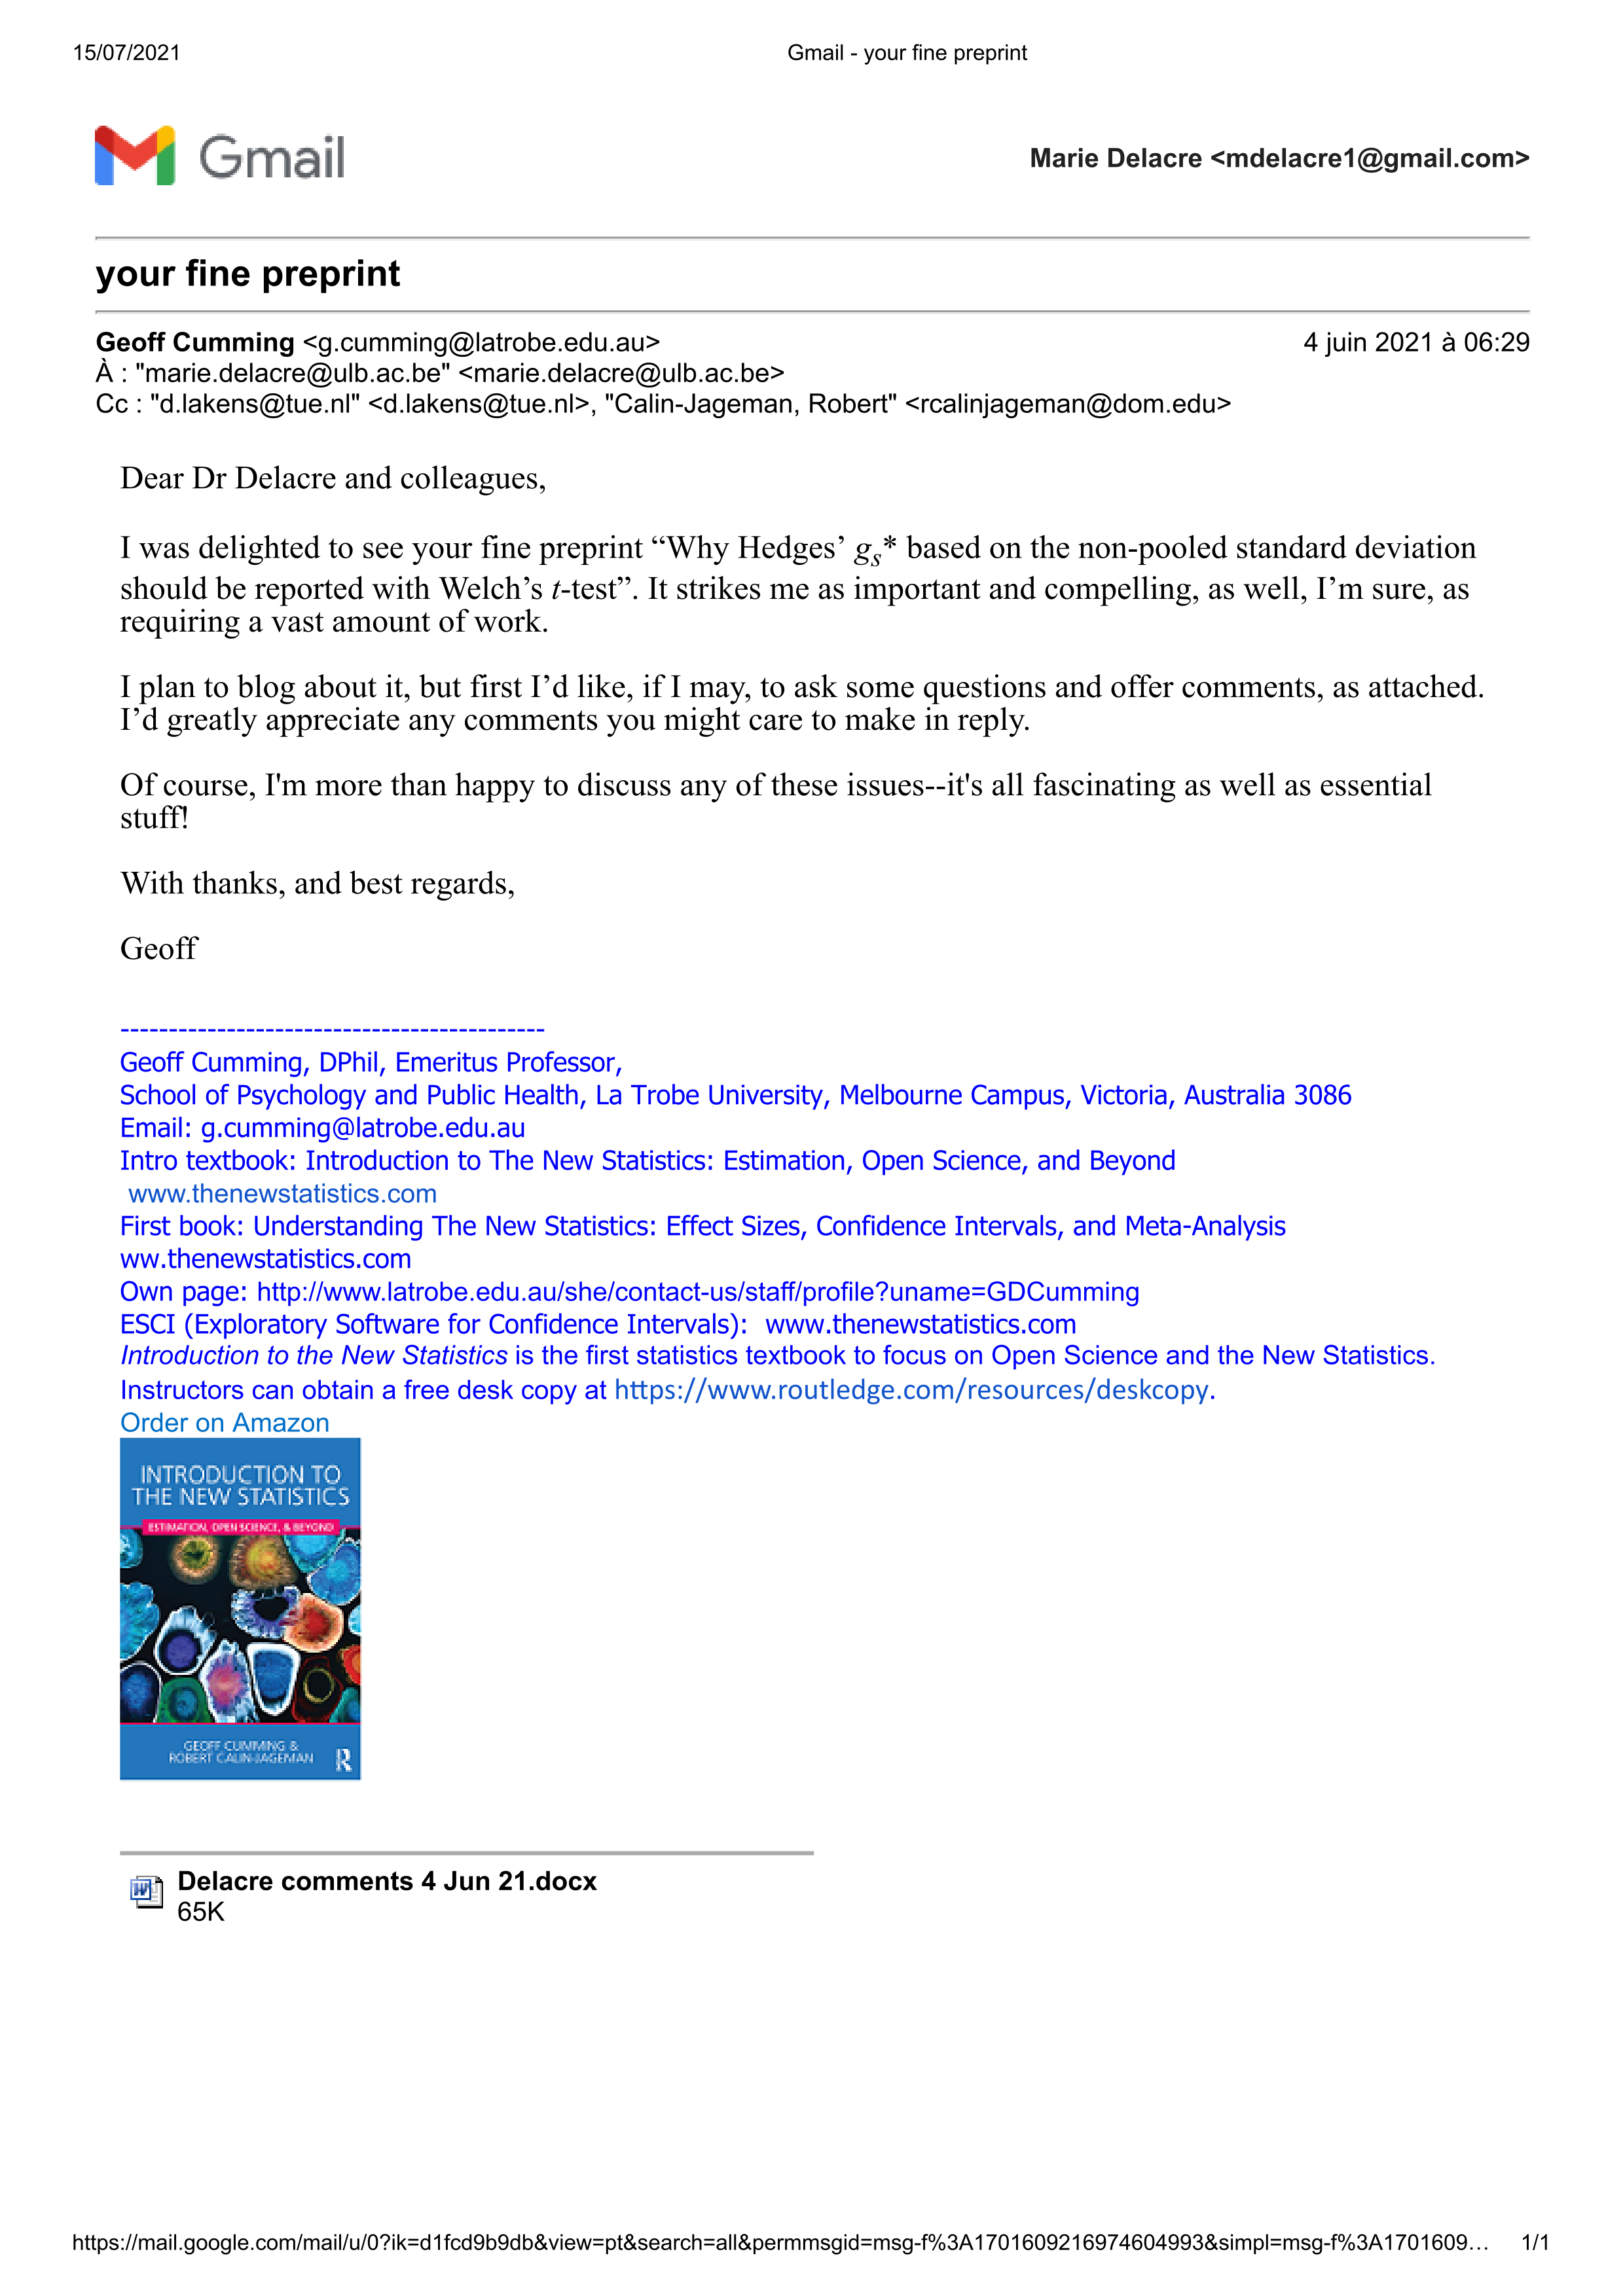
\includegraphics{C:/Users/Admin/Documents/Github projects/thesis/Chapitre 4/Echanges avec Cumming/Cummingmail1.png}
\newpage

\begin{center}\rule{0.5\linewidth}{0.5pt}\end{center}

\color{black}\textbf{Why Hedges' \(\bm{g_s^*}\) based on the non-pooled
standard deviation should be reported with Welch's \(\bm{t}\)-test}

\underline{https://psyarxiv.com/tu6mp/}

Comments by Geoff Cumming\\
\underline{g.cumming$@$latrobe.edu.au}

4 June 2021

\textbf{Subscript \emph{s}}

I'm wondering why you use subscript \(s\) for all eight ES measures.
Yes, Cohen's original term for the estimate was \(d_s\), but \(d\)
became the standard usage. Perhaps you use the subscript \(s\) to
indicate that the standardiser is an \(SD\) estimated from data? By
contrast \(d_\delta\), for example, would indicate that a population
value is available to use as standardiser. But in your paper there are
no such cases, so you could simplify everything by simply omitting all
those subscript \(s’\)s?

Also, that role for the subscript rules out use of it to distinguish,
for example, between \(d_p\) for pooled \(s\), and \(d_C\) for Control
group \(SD\) as standardiser. However, I know there are no
well-established conventions for such subscripts, and you need to use
`Shieh' as a label for those ES measures, so perhaps using name labels
(Cohen's, etc) for all measures---as you do---and dropping all the \(s\)
subscripts would be simplest.

\color{blue} I used the subscripts to indicate that the ES measure is
estimated based on a sample, but I agree that it is maybe not necessary,
so I will remove all subscripts and use labels instead.

\color{black} \textbf{Typos?}

\color{blue} Thanks for pointing all these typos out!

\color{black} p.~7, l. 139: Hedges' \(d_s^*\) should be Cohen's
\(d_s^*\)? \color{blue}That's right, it should be Cohen's \(d^*\)

\color{black} p.~8, l. 152: Use \(\sigma\) rather than
\(\sigma_{pooled}\) (twice) because here we're assuming homogeneity of
variance, with \(\sigma = \sigma_1 = \sigma_2\) as the common population
\(SD\)? (Also Table 1, line 1 of Note.) \color{blue} \color{blue}Ok!

\color{black} p.~9, l. 3 of footnote: Not 52 but .52? (By my calcs using
\(df = 3\), \(N = 5\), and the approximate debiasing formula the value
should be .529?) \color{blue} Yes, it's a typo, the right number is .52
instead of 52 (see the R console below).

\includegraphics{C:/Users/Admin/Documents/Github projects/thesis/Chapitre 4/Echanges avec Cumming/printscreen.png}\\
\color{black} Table 3: Cohen's \(g_s^*\) should be Hedges' \(g_s^*\)?
Also on p.~20, l. 275 (without *), and p.~30, l. 485. \color{blue} Also
true.

\color{black} \textbf{Non-normality}

It's great that you explore non-normality, so that you are investigating
the robustness of the various ES estimators. I'd love to see a figure
showing the three example distributions you choose to study, alongside a
normal curve. Then I could have some intuitions about how extreme they
are, especially in comparison with distributions that I might see in
data I'm analysing. Thanks.

\color{blue} In the plot below, here is what the four distributions look
like when \(\mu = 0\) and \(\sigma = 1\).

\includegraphics{C:/Users/Admin/Documents/Github projects/thesis/Chapitre 4/Echanges avec Cumming/printscreen2.png}\\
It is a nice suggestion to add a Figure in the manuscript to show the
compared distributions, I will take it into account.

Additional comment: in our simulations, we used only continuous
distributions. I think it would be interesting to test the properties of
estimators when distributions are discrete (e.g.~Likert scales) but I
have no idea how to generate such distributions in a realistic way. If
you have any suggestion, I would be more than happy to think about it
next time!

\color{brown} Yes, it would be valuable to have investigations with
discrete distributions, but I can't think of good starting points. We'd
hope for better than the normal approximation to the binomial. Maybe
start with the investigations that have been made of that, especially
with small N (Likert, as you mention).

\color{black}\textbf{Bias}

I take your point (p.~23) about the value of focusing on relative,
rather than absolute, bias (and variance) when there is a change in
measurement units. But that doesn't happen in your investigations.

\color{blue} Well, I wrote about a ``change of unit'' because we use a
different standardizer for each estimator. As a consequence, each
estimator computation results in a different value in order to describe
the same amount of difference. I will clarify in the text.

\color{black} The one other reason you state for considering relative
bias is a reference, on p.~5, bottom, that Tables 1 and 2 illustrate
that ``bias is directly related to the population effect size''. That's
true for Cohen's \(d\) in Table 1, and for \(d\) and \(d^*\) in the top
two rows of Table 2. (I'm omitting Shieh from my comments---see below
for reasons.) The debiasing that gives Hedges' \(g\), etc, is
proportional, and results in zero bias for any population effect size. I
think, therefore, that neither of the reasons you mention for using
relative bias applies for any of the \(g\) family measures in Figures
2-9 (omitting Shieh, as I will do unless specifically mentioned), and so
I'm wondering whether seeing means (i. e., averaged over \(\delta\)
values) of relative or absolute bias would be more informative.

\color{blue} I agree that under the normality assumption, there is no
bias for any unbiased estimator, of course. However, when the normality
assumption is not met, biases occur. In Supplemental Material 1, we
mention that when samples are extracted from heavy-tailed symmetric
distributions, this bias depends on the same parameters as the bias of
biased estimators when the normality assumption is met. It's true that
we mainly based our decision to compute the relative bias on the
comparison between Cohen's \(d\) (Hedges' \(g\)) and Shieh's \(d\)
(Shieh's \(g\)). For example, when designs are balanced and population
variances are equal across groups, the bias of Shieh's \(g\) is always
approximately twice smaller as the bias of Hedges' \(g\), and its
variance is always approximately four times smaller as the bias of
Hedges' \(g\). It gives the illusion that under this specific
configuration, Shieh's \(g\) is less biased and variable as Hedges'
\(g\), but it is only due to what we called ``a change of unit''.

Note: I explain below why I think it's important to consider Shieh's
\(d\) in our comparisons (even if I agree with the fact that
interpreting this measure is very hard).

\color{black} I guess I'd like to see the bias for each \(\delta\)
value. (On p.~24, line 2, you give a link to an illustration of raw bias
and variance, but I can't find any tables or graphs of values at that
site.)

\color{blue} The graphs for raw estimators of goodness are available on
my Github account:\\
\underline{https://github.com/mdelacre/Effect-sizes/}.\\
You will find them in the following folder: ``Scripts outputs/Quality of
ES measures/Graphs/Unbiased estimators/Raw estimators of goodness/''.
The fact that you haven't found it probably means that I should
reorganize the folder, in order to make it clearer, to indicate more
clearly the Figures position in the folder or to add a read me file!

\color{brown} Thanks for the link for raw results.
\url{https://github.com/mdelacre/Effect-sizes/} That's different from
the link in the preprint. \color{darkgray}{[}En effet, nous avions collé
un mauvais lien par erreur dans le preprint{]}.

\color{black} You say that the main purpose of the figures is to allow
comparisons between the different ES measures, rather than absolute
values for bias (and variance). Even so, knowing when bias is likely to
be absolutely small or large can inform judgments about the different ES
measures in various contexts. In Figures 2 and 3, we have
\(\sigma_1=\sigma_2\) and four versions of \(g\), all debiased. If I'm
following, the relative bias values pictured in the top rows of both
figures are averaged over \(\delta\) = 1, 2, 3, and 4. (I'm assuming
\(\sigma_1=\sigma_2=1\); correct?) \color{blue} Right! \color{black} For
the non-normal distributions, average relative bias in the best cases is
around 1-2\(\%\), so not bad. But up to around 5-10\(\%\) in some other
cases, a bit more concerning.

\color{blue} Absolutely right. However, as mentioned in the manuscript,
``we chose very extreme conditions, and we know that none of the
parametric measures of ES will be robust against such extreme
conditions''. It is therefore not surprising that \emph{all} estimators
are very large under some conditions. We could insist more on the fact
that the parametric estimators are robust only under moderate deviations
from the normality assumptions.

\color{black} It's interesting to see that almost all the relative bias
values plotted in Figures 2-9 are positive, so in nearly all cases the
ES estimates are on average too high? If so, this may be worth noting?
(Apologies if I missed your comment on this.)

\color{blue} You're perfectly right. There is a mathematical reason for
that (at least for symmetric distributions; it is explained in
Supplemental Material 1, in the ``Preliminary note''; see below). We did
not include this note in the main manuscript because we were afraid that
it would be too technical for many psychologists, and we did not want to
complicate even more a paper that already contains many complex
concepts, but maybe we could mention this in a footnote if you think
it's missing.

\includegraphics{C:/Users/Admin/Documents/Github projects/thesis/Chapitre 4/Echanges avec Cumming/printscreen3.png}\\
\color{black} \textbf{Variance}

For bias, the goal is zero, an unbiased estimate. For relative variance,
the smaller the better, but we don't expect zero because we'll always
have sampling variability in estimates of \(\delta\). I'm finding it
hard to think of a good way to get intuitions about the empirical
variances of the different ES measures, starting with the relative
values reported in Figures 2 and 3. Part of my difficulty is that
variance is a squared measure. As usual, I'd much prefer to be able to
think in terms of CIs and their lengths.

\color{blue} Thinking in terms of CIs and their lengths require to run
new simulations because we compute CIs based on the noncentral t
distribution method (the method is explained in CI.pdf, here:
\url{https://github.com/mdelacre/Effect-sizes/tree/master/Supplemental\%20Material\%204/CI.pdf/}
; the R script is available here:
\url{https://github.com/mdelacre/Effect-sizes/blob/master/Scripts/Confidence\%20intervals/CI.R}.

I have made simulations in order to compute CIs around point estimators
for all scenarios where \(\mu_1-\mu_2 = 0\) and \(\mu_1-\mu_2 = 1\).

Note that analyses on CIs would probably be very redundant with that of
the variance. I agree that the length of CIs is probably more intuitive,
but at the same time, everybody knows that the variance is a measure of
dispersion, and the greater the variance, the greater the dispersion. We
mention that our main goal is to \emph{compare} the relative bias and
variance of different estimators, and variance allows this comparison.

\color{black} The variance formulas in Tables 1 and 2 show that the
variance of \(d\) and \(g\), and the top two ES measures in Table 2, do
indeed depend on \(\delta\). To try to get a feel for the extent of this
dependence I made a quick spreadsheet of the variance formula for
Cohen's \(d\), using the approximate formula in the second line of Table
1. The figure below shows the percentage of variance in \(d\) that is
given by the second, \(\delta\)-dependent, term in the formula for
variance. I assumed two equal sized groups. The figure suggests that for
\(\delta<1\) only a very small \(\%\) of the variance is dependent on
\(\delta\), and for \(\delta=1\) (around 10\(\%\)) and greater, the
\(\%\) increases rapidly with \(\delta\)---not surprisingly, given the
\(\delta^2\) term in the formula. The \(\%\) hardly changes with sample
size, for two samples each of at least 20, as you use.

\includegraphics{C:/Users/Admin/Documents/Github projects/thesis/Chapitre 4/Echanges avec Cumming/printscreen4.png}\\
For \(\delta\) values of 1, 2, 3, and 4 (as are averaged in Figures 2,
3), the \(\%\)ages are, in round numbers, about 11, 34, 54, and 67,
respectively. I expect the \(\%\)ages for the other ES measures would
not be vastly different. Therefore the relative variance values shown in
the lower row in Figures 2 and 3 are averages over cases in which
dramatically different proportions of the variance are dependent on
\(\delta\). I think this makes it harder to get good intuitions. Values
of the variance of the estimates, rather than relative values, may be
more understandable?

\color{blue} This is a very interesting analysis. I was quite confused
about this question, and I've been wondering for a long time what the
best solution would be. We had many long discussions in order to decide
whether we should compute the variance or the relative variance. The
issue was indeed the fact that the variance only partly depends on
delta. Finally, we decided to compute the relative variance because we
had in mind that when \(n_1=n_2\) and \(\sigma_1=\sigma_2\), the bias
(variance) of Shieh's \(d\) is twice smaller (four times smaller) as the
bias for Cohen's \(d\), only because Shieh's \(d\) is twice smaller as
Cohen's \(d\) (see Appendix 1 in our paper). However, I keep in mind
that you argue in favor of removing Shieh's \(d\) from our analyses.

\color{black} Taking a different approach, and considering the relative
variance values plotted in Figures 2 and 3, would it be reasonable to
say that relative \(SD\), the square root of relative variance, is the
\(SE\) used to calculate the CI on that ES estimate, expressed as a
fraction of \(\delta\), the population ES? If so, such a 95\(\%\) CI
would be about \(\pm 2 \times SE \; value \times \delta\). (Given that
the smallest total \(N\) being considered is 40, that approximation
should be reasonable? Perhaps less so for much smaller group sizes. The
asymmetry of CIs on \(d\) is actually very small unless \(N\) is very
small and \(\delta\) is large.) If that's at least roughly correct, then
your reported values of average efficiency become indicators of the
precision of the different ES estimates. An efficiency estimate (lower
row in the figures) of, say, 0.04 (a typical low value) would correspond
approximately to \(SE=0.2\delta\) and a 95\(\%\) CI of about
\(\pm 0.4 \delta\). However, that's very rough because the efficiency
values plotted are means of four possibly quite different values. (The
dependence of relative variance---and thus CI length---on \(N\) is clear
in Figure 2, and can also be seen in Figure 3.)

\color{blue} This is not very clear to me. If you think this is a key
point, perhaps we could discuss it together when I will revise the
article?\\
\color{brown} It looks complicated here but, I think, mainly because I'm
trying to get approx CI info from averaged relative variance values.
It's probably not worth considering this further, given that somewhere
in future plans may be analyses that tell us directly about CI lengths
and coverage \%ages, and likely errors (biases) in these. I'm more than
happy to discuss at revision time.

\color{black} \textbf{Shieh's \emph{d} and \emph{g}}

I can see that including these does give a comprehensive exploration of
ES possibilities. Seeing them here led me to go back to Shieh's original
article and my comment. You cite that comment (thank you) as reason to
doubt the value of the Shieh approach. You also point out (p.~15,
bottom) that in the base case the Shieh value is half \(d\). This seems
to me so crazy that it alone may provide sufficient reason to dump the
Shieh approach. For example, a difference of 7.5 between two IQ means is
\(d\) = 0.5, half an \(SD\). That makes sense. But Shieh would calculate
0.25! Units of double the SD! How could we make sense of that? How could
I even attempt to justify that to students as a meaningful standardised
ES measure?

But as you say there's more. Calculating a pooled \(SD\) weights by
sample size, for good reasons. The Shieh calculation, however
counter-weights, so the \(SD\) of the \(smaller\) group is weighted more
heavily. That's what we need to calculate the variance, but, surely, not
a value that could justifiably be used as standardiser---the units in
which to express our standardised ES.

Even more, again as you say: Simply change the \(n\)-ratio and the
\(SD\) estimate changes, so we can't see the ES value we get as an
estimate of any readily understood population quantity.

All that seems to me more than enough reason simply to dump the Shieh
approach. Imho, it's worth no more than a para or two to explain why
it's not worth pursuing.

\color{blue} I get your point and I agree with all what you say. At the
same time, Shieh's \(d\) is based on the same statistical quantity as
Welch's \(t\)-test. By ``same quantity'', I mean that the percentage of
\(p\)-values associated with Welch's \(t\)-test below the alpha risk
exactly equals the proportion of confidence intervals around Shieh's
\(d\) that does not include 0. Our first motivation to write this paper
was to advice researchers with a measure they could use when performing
Welch's \(t\)-test, in the continuity of our previously written articles
on the subject (``Why Psychologists Should by Default Use Welch's
\(t\)-test Instead of Student's \(t\)-test'' and ``Taking Parametric
Assumptions Seriously: Arguments for the Use of Welch's \(F\)-test
instead of the Classical \(F\)-test in One-Way ANOVA''). In that
context, I think it's a bit weird to not include this effect size
estimator in our comparisons. Moreover, before running all my
simulations, I thought that this test was the best from an inferential
point of view (again, due to this mathematical relation). The study of
bias and variance reveals that even for inference, it has big flaws. For
that alone, I find it interesting to include it in the comparisons. At
the same time, we can (and we will) insist a little more on the fact
that the mathematical relation between Welch's t-test and Shieh's d
explains why we took this ES estimator into account, and specify at the
outset that the simulations will reveal that this measure is not very
defensible, even purely statistically speaking.

\color{black} \textbf{Results section} p.~24, ll. 356-8: moving left to
right, columns 2-4: in both figures the bias increases slightly then
decreases considerably---not ``moving left to right\ldots{} the larger
the bias''

\color{blue} Have you noticed that in column 4, we don't use the same
scale as in column 2 and 3 (this is true for both Figures 2 and 3)? So
indeed the bias is larger in column 3 than in column 2, and larger in
column 4 than in column 3.

\color{brown} In some places I did note the differing vertical scales in
your figures, esp.~Column 4. But I slipped up in my comments on
interpretation of those figures. Sorry.

\color{black} p.~27, l. 403: Unequal variances. In Figure 4, what are
the variances? A single pair of values in all cases, or are the pictured
values averaged over a range of variance pairs?

\color{blue} Scenarios in Figure 4 are those where \(\sigma_1\) always
equals 1, and \(\sigma_2\) = .1, .25, .5, 2, 4 or 10, so pictured values
are averaged over a range of variance pairs. I'll mention it explicitly
in the next version to avoid confusion.

\color{black} p.~27, ll. 407-8: ``when moving from left to right\ldots{}
the larger the bias''. But for all Figures 4-9, except 7, bias increases
slightly (or hardly) from column 2 to 3, then drops to be smallest in
column 4.

\color{blue} Again, we don't use the same scale in column 4 vs.~columns
2 and 3. It was mentioned p.24, l. 339.

\color{black} p.~27, ll. 408-9: ``the bias of Hedges' \(g_s\) remains
very small\ldots{}'' But it is often large, and in every case no smaller
than that of Hedges' \(g_s^*\).

\color{blue} I meant that the bias of Hedges' g remains very small when
the normality assumption is met (but this needs to be clarified better
in the sentence!).

\color{black} I'm wondering what value you use for \(\delta\) when
assessing relative bias and variance for Hedges' \(g\). Perhaps what you
define for \(\delta_{Cohen}\) back on p.~8, l. 152? If so, that value
depends not only on the two variances, but on the two sample sizes. So
we're estimating a population ES that doesn't reflect any relevant
population in the world and, moreover, assuming a population ES that
changes merely because we happen to use different sample sizes.

\color{blue} What would you recommend to use? Indeed I'm using
\(\delta_{Cohen}\). Mathematically speaking, the expectation of Hedges'
\(g\) always equals \(\delta_{Cohen}\) when both assumptions of
normality and equal population variances are met, so we compare
mean(Hedges' g) with \(\delta_{Cohen}\) in order to compute the raw
bias. This explains why I also used \(\delta_{Cohen}\) in the
denominator when I computed the relative bias.

\color{brown} I had in mind the introduction of Cohen's d on pp.~7-8. We
are assuming homogeneity of variance. I made a comment:\\
p.~8, l. 152: ``Use \(\sigma\) rather than \(\sigma_{pooled}\) (twice)
because here we're assuming homogeneity of variance, with
\(\sigma = \sigma_1 =\sigma_2\) as the common population \(SD\)? (Also
Table 1, line 1 of Note.)'' Ok!

\(\rightarrow\) you agreed with that. So the formula, line 152, with the
square root (I'll call that `the weird formula') reduces to
\(\sigma = \sigma\). I guess I'm assuming that Cohen's \(d\), and also
Hedges' \(g\), are defined assuming homogeneity of variance and their
formulas use \(s_p\), the pooled value. They both estimate \(\delta\),
defined as in your (5).

Thinking further about this, I take your point. In a simulation we know
\(\sigma_1^2\) and \(\sigma_2^2\), as well as the two sample sizes, but
we know of no `true' single \(\sigma\) to use in defining the \(\delta\)
we would like to use as the benchmark to assess the estimates calculated
in the simulation. Perhaps using the weird formula is the best we can
do; if anything using this means we're bending over backwards to
minimise likely estimation error.

Perhaps you could consider shifting the weird formula from the basic
intro to Cohen's \(d\) on pp.~7-8, where to me it doesn't seem to fit,
and introducing it, as a sort of necessary evil, when explaining the
simulation evaluation of \(d\) and \(g\)?

\color{black} However, on p.~27, from l. 411, you say that pooling
variance estimates in this situation results in an {[}effect size{]}
estimator that ``will be smaller\ldots{} or larger\ldots{} than it
should be.'' What should it be? Doesn't such an estimator match the
definition of \(\delta\) I refer to above? Then you make the same
statement about population values, although that would not be true if
you are using the definition of \(\delta\) I refer to above---which is
based on just such a pooled (and weighted by sample size) population
\(SD\)? Even so, your conclusion at the top of p.~28, dismissing Hedges'
\(g\), may be justified---when variances differ.

\color{blue} I'm not sure that I understand your comment. Could you
please clarify? P.27, we meant that when variances are unequal across
populations, the pooled error term is not valid (because it assumes
equal population variances). When we compute the bias of Cohen's \(d\)
in scenarios with unequal population variances, we compare an invalid
estimate with an invalid population measure of effect size. Because both
estimate and population value are invalid, the problem of Cohen's \(d\)
in case of heteroscedasticity is not revealed by the calculation of the
bias. This is actually the same explanation as p.10:

\includegraphics{C:/Users/Admin/Documents/Github projects/thesis/Chapitre 4/Echanges avec Cumming/printscreen5.png}\\
\color{brown} Given your explanation about using the weird formula, I
think I now understand what you were getting at. Your statement that the
estimate and the population measure (calculated using the weird formula)
are both invalid expresses the problem that there's probably no good way
to calculate the population measure when variances are unequal. No
sensible way to specify what the estimate should be estimating. Indeed!

Of course, if we try to avoid the double invalidity you point to by
simply averaging the two different \(\sigma\) values, we get the \(d^*\)
and \(g^*\) estimators. These may solve the unequal \(n\) problem of the
weird formula, but still have problems (in my view, severe problems) in
terms of interpretability.

\color{black} p.~28, l. 422: ``parameters that we cannot
control\ldots{}''. You include the \(n\)-ratio, which is true if, for
example, we are meta-analysing past research. But in many cases a
researcher chooses sample sizes, and your investigations are likely to
lead to useful advice about choice of sample sizes.

\color{blue} I think it's partly true. About the bias, the larger the
control group size, the lower the bias. About the variance, it's a bit
more complex: in Supplemental Material 1 we write that when the
normality assumption is met ``The variance always decreases when the
control and/or the experimental group increases. The benefit of adding
subjects in the control, in the experimental, or in both groups, in
order to reduce the variance, varies as a function of the \(SD\)-ratio
and the population effect size. The only situation where it is optimal
to maximize the experimental group is when \(\sigma_e>\sigma_c\) and
\(\delta_{Glass}\approx 0\). Most of the time, it is more efficient to
maximize the control groups (e.g.~anytime \(\sigma_e<\sigma_c\), and
when \(\delta_{Glass}\) is very large) or to uniformly add subjects in
both groups (e.g.~when \(\sigma_e>\sigma_c\) and \(\delta_{Glass}\) is
neither null nor huge)'' (This is a summary but you can see more details
and figures here:
\url{https://github.com/mdelacre/Effect-sizes/blob/master/Supplemental$/\%$20Material$/\%$201/Theoretical$/\%$20Variance$/\%$20of$/\%$20all$/\%$20estimators$/\%$20as$/\%$20a$/\%$20function$/\%$20of$/\%$20population$/\%$20parameters.pdf}
).

As we can see in this summary, recommendations about sample sizes would
be different as a function of \(SD\)-ratio and most of the time, we
don't know the \(SD\)-ratio in advance. But thanks for pointing this
out, it probably deserves at least a footnote!

\color{black} \textbf{Discussion}\\
I think your three purposes of ES estimators (pp.~3-4) are spot on. Your
three desirable properties are indeed the desirable statistical
properties, but I'd list interpretability in the research context as the
first essential property. If we don't have interpretability for a
particular standardised ES estimator then we shouldn't be using it.

\color{blue} Theoretically speaking, I agree with you. But practically,
as I've mentioned before, I'm not sure if it's a good idea to rule out
an estimator that has such a direct connection to Welch's \(t\)-test. It
is probably possible to introduce things differently, to explain in
advance that the Shieh's \(d\) is not desirable (and to add that even
from an inferential point of view, it has big flaws).

Apart for that, you're right, interpretability should be our first
priority. For example, if we don't have an interpretable measure, we
cannot use it in order to make informative null hypothesis (e.g.~when
performing equivalence test). However, I'm a bit concerned with the fact
that interpretability and good inferential properties seem so difficult
to reconcile. How could we interpret an estimator correctly if it is
very biased? This makes me very reserved about Glass's \(d\).

\color{black} I note these recommendations:

\begin{enumerate}
\def\labelenumi{\arabic{enumi}.}
\tightlist
\item
  p.~10: ``Because the assumption of equal variances\ldots{} is rarely
  realistic\ldots{} both Cohen's \(d\) and Hedges' \(g\) should be
  abandoned\ldots{}''. I think that's arguable. I'm not convinced that
  assumption is rarely realistic. The assumption is very often made, for
  example, I think, in medicine when calculating SMD. I suspect a large
  proportion of Cochrane systematic reviews include meta-analyses that
  make this assumption. Of course that doesn't make it justified in
  every situation, but I suggest the emphasis should be on informed
  judgment in context rather than simply abandoning these ES estimates.
\end{enumerate}

\color{blue} Perhaps do we need to be more nuanced in asserting this.
However, there are many authors who believe that the assumption of
homogeneity of variances often does not hold (see for example Erceg-Hurn
\& Mirosevich, 2008; Zumbo \& Coulombe, 1997). In a previous paper
(Delacre et al.~2017) we develop many reasons why we think equal
population variances are very rare in practice.

Moreover, it's very hard to check for the homogeneity of variances
assumption, because:\\
* the assumption is about population parameters that we don't know
(\(\sigma_1\) and \(\sigma_2\));\\
* inferential statements about the homogeneity of variances assumptions
based on assumptions tests often lack power to detect assumption
violations.

Finally, when we look at figures, we notice that when variances are
equal across groups, Cohen's \(g\) and Cohen's \(g^*\) are either
identical (Figure 2) or very close (Figure 3). The only exception is
when both skewness and kurtosis are very large (as reminder, we used
different scale in the fourth column in comparison with all other
columns). Most of the time, there is therefore little cost in choosing
Cohen's \(d^*\) by default. On the contrary, Cohen's \(d\) cannot be
used in case of heterogeneity of variances. -- Delacre, M., Lakens, D.,
\& Leys, C. (2017). Why psychologists should by default use 521 Welch's
t-test instead of Student's t-test. International Review of Social
Psychology, 522 30 (1), 92--101. \url{https://doi.org/10.5334/irsp.82}

-- Erceg-Hurn, D. M. \& Mirosevich, V. M. (2008). Modern robust
statistical methods: An easy way to maximize the accuracy and power of
your research. American Psychologist, 63(7), 591. DOI:
\url{https://doi}. org/10.1037/0003-066X.63.7.591

-- Zumbo, B. D. \& Coulombe, D. (1997). Investigation of the robust
rank-order test for non-normal populations with unequal variances: The
case of reaction time. Canadian Journal of Experimental Psychology/Revue
Canadienne de Psychologie Expérimentale, 51(2), 139. DOI:
\url{https://doi}. org/10.1037/1196-1961.51.2.139

\color{black}

\begin{enumerate}
\def\labelenumi{\arabic{enumi}.}
\setcounter{enumi}{1}
\tightlist
\item
  pp.~17-18: You note the wide criticism of Cohen's \(d^*\) (and by
  implication Hedges' \(g^*\)) because the standardiser is not the
  \(SD\) of an existing relevant population. You state that, even so,
  these estimators have very good inferential properties. Grissom and
  Kim (2012), referring to this averaging of variances, state that we
  ``are estimating the \(\sigma\) of a hypothetical population\ldots{}
  which is a concern for some \ldots{} but not others'' (p.~72). I tend
  towards the concerned end of that range, but I know there are
  arguments in favour of using the square root of the average of two
  different variances as standardiser. Maybe it can sometimes be
  possible to give a reasonable interpretation using such a strange
  standardiser. Think of two overlapping normal curves with different
  \(SD\)s: What \(SD\) unit is best for expressing the difference
  between the two means? Does it make sense to use a compromise between
  those two \(SD\) values? Again, this should be recognised as a
  judgment call, and lack of interpretability in context should never be
  over-ruled by good statistical properties.
\end{enumerate}

\color{blue} I find this convincing (especially the fact that
interpretability should never be over-ruled by good statistical
properties) and will have to think about a better way to introduce this
estimator.

\color{black}

\begin{enumerate}
\def\labelenumi{\arabic{enumi}.}
\tightlist
\item
  p.~28, l. 424: ``We do not recommend using {[}Glass's \(g\){]}.'' I
  suggest that Glass vs something else is the choice that most clearly
  should be based on the context. Does it make sense to use the \(SD\)
  of one group as the standardiser? If so, we should do so, unless there
  are very strong reasons against. We should use choice of sample sizes
  and perhaps other strategies to minimise any disadvantage of the Glass
  ES estimate. You make several observations that can help, mainly that
  increasing the control group sample size is desirable.
\end{enumerate}

\color{blue} As previously mentioned, we need to increase the control
group in order to reduce the bias, but sometimes, we need to increase
the experimental group in order to reduce the variance. This makes
recommendations about sample sizes very complicated.

\color{black}

\begin{enumerate}
\def\labelenumi{\arabic{enumi}.}
\setcounter{enumi}{1}
\tightlist
\item
  p.~30, l. 473: ``We recommend using Hedges' \(g^*\)\ldots{}'' You
  state some strong advantages of this ES estimator, but I remain
  hesitant because of the possible interpretive difficulty, given its
  standardiser.
\end{enumerate}

Overall, you provide a wonderful range of detailed findings. I'd love to
see you develop the discussion, drawing further on those findings, in a
way that guides a researcher's likely full decision sequence. For
example, first, do we have some relevant population \(SD\) value? If so,
use this as standardiser. If not, Glass or something else, considering
the context? If not Glass, homogeneity of variance or not? Then, can we
improve the precision of estimation of our chosen standardiser by, for
example, pooling over studies, or meta-analysing our data with past
research? Meaningfulness and interpretability in the context should
always be the primary consideration.

The great value of your findings is then to help us be specific about
the trade-offs. If I choose Glass, how large is the likely bias? If only
a few \(\%\) I might be prepared to tolerate that, or I might consider a
data transformation to reduce the departure from normality. (Perhaps a
log transform of RT data?) Of course, all such choices should where
possible be made in advance of seeing the data, when formulating the
data analysis plan to be preregistered.

\color{blue} This is a set of considerations that I will have to take
into account when I rework my article in September. If you're ok with
that, I'd love to show you our next draft before submitting it.

\color{brown} I'd be more than happy to comment on future drafts, in due
course. Or to discuss any of these fascinating issues!

\color{black} Earlier I made a very sketchy attempt to estimate roughly
what CI length might be, given your relative variance results. You refer
(e.g., p.~17, l. 253) to ``very good inferential properties''. That's
highly relevant, but I suggest CI length and coverage should be central
issues in assessing the inferential effectiveness of any estimator.
Then, when considering some judgment call, I could weigh up any price
there might be to pay in terms of a longer CI for one of the options
under consideration, or a slight departure from 95\(\%\) coverage. No
doubt investigation of CI length and coverage would be a further
project, although perhaps you could derive from your variance results
some relevant guidance based on CIs?

Ideally, we'd like to see the performance of CIs based on non-central
\(t\) distributions, and also bootstrapped CIs, for the various
estimators and conditions you investigate. Ideally, again, we could then
weigh up the various choices, with some idea as to the cost in terms of
bias or CI length or coverage error of a choice that offers superior
interpretability---which should always be paramount.

\color{blue} As mentioned above, I already computed CIs for all the
conditions, based on non-central \(t\) distributions. However, I haven't
analyzed them yet but I could use them in order to compute the coverage
probability and CI length. Therefore these comments could be part of the
``further studies'' section, and be the subject of a second paper.

\color{black} Overall, your investigations give us highly valuable
findings to guide such discussions.

\textbf{Title}

Current title: ``Why Hedges' \(g_s^*\) based on the non-pooled standard
deviation should be reported with Welch's \(t\)-test''.

Why mention that \(t\)-test? Yes, it fits with your message that the
assumption of homogeneity of variance should be avoided, but it's hardly
mentioned in the paper, and if an ES estimate and CI are reported
there's no need to report or even mention any \(t\)-test. I would argue
that it's much better to avoid doing so.

More positively, your investigations warrant broader recognition and
description. Perhaps something like: ``\(d\)-family standardised effect
size estimators: Interpretability, bias, efficiency, and robustness''
``\(d\)-family standardised effect sizes: Bias, efficiency, and
robustness'' ``Cohen's \(d\) and related effect size estimators:
Interpretability, bias, precision, and robustness'' {[}my current
favourite; assumes some discussion of CIs{]} ``Cohen's \(d\), Hedges'
\(g^*\), and related effect size estimators: Interpretability, bias,
precision, and robustness'' {[}includes the largest set of terms likely
to be used in an online search{]}

\color{blue} We wanted to mention \(t\)-test because this answering the
question many people asked us: Which effect size should I report for
Welch's \(t\)-test. Yes, the paper discusses more, adding
Interpretability, bias, precision, and robustness is a good addition.
What do you think about: ``Arguments to use the Hedges'\(g_s^*\) with
the Welch's \(t\)-test: an investigation of interpretability, bias,
precision, and robustness of d-family effect sizes''?

\color{brown} As I said in the blog post, \color{darkgray} {[}Voir lien
vers le blog post{]} \color{brown} I'm not convinced that Welch's
\(t\)-test deserves mention, even though you have made a strong case for
using that form of the \(t\)-test in your earlier paper. If people ask
`which \(ES\)?' I'd answer that they need to make a judgment in context,
partly guided by your robustness results---but I've said all that in the
post.

I know that you make a general recommendation that, when variances are
or may be unequal, we should use Hedges' \(g^*\), and, separately,
Welch's \(t\)-test, but I don't see any other link between the two.

Your Equation (10), p.~15, expresses the very strong link between
Welch's \(t\) and Shieh's \(d\). Somewhere I've read a statement that
the CI on Shieh's \(d\) corresponds with Welch's \(t\) test in the sense
that the two give the same \(p\) values, tho' I can't find that
statement in Shieh (2013) or in your preprint or supp material---sorry
if I've missed it. However, I'd expect that the CI on your recommended
Hedges' \(g^*\) and Welch's \(t\) would not give the same \(p\) values.
If that's correct, we have one more reason not to link the two together,
for example in the title.

\color{black} Grissom, R. J., \& Kim, J. J. (2012). \emph{Effect sizes
for research}, \(2{nd}\) ed.~New York: Routledge.

\color{brown} It's nice to see a bunch of likes and retweets to the
tweet about the blog post. \color{darkgray} {[}See
\underline{https://twitter.com/TheNewStats/status/1405386935074496512}{]}

\color{brown} There's a useful comment (link below) from Brenton Wiernik
about relevant work by Doug Bonnett. Very likely you know this, tho'
it's new to me. I'd better have a squiz.

Cheers, Geoff\\
\color{black}
------------------------------------------------------------

\newpage

\hypertarget{annexe-d-a-voir-si-erratum-du-chp-5}{%
\subsection{Annexe D: A VOIR SI ERRATUM DU CHP
5?}\label{annexe-d-a-voir-si-erratum-du-chp-5}}

\end{document}
